\documentclass[fancy,estyle,twoside,a4paper]{ethesis}

%The following two packages are required to have awesome font qualities!
\usepackage[T1]{fontenc}
\usepackage{ae,aecompl} %,placeins

% ========== Mathematics 

\usepackage{amsmath,amssymb,amstext,amsthm}
\numberwithin{equation}{section}




\usepackage[round]{natbib}

% ========== Color

\usepackage{color,soul,bm}
\usepackage{colortbl}
\usepackage[normalem]{ulem} %to have nice underlining, for exmaple try \uwave{blahblah}

\usepackage{graphicx}

\usepackage{fancyhdr}
\usepackage{lettrine} %Typeset dropped capitals

% ========== Algorithm

\usepackage[chapter, ruled]{algorithm}
\usepackage{algorithmicx}
\usepackage{algpseudocode}
\usepackage{color}

\usepackage{bibentry}
\nobibliography*

% ========== Figures
  
\usepackage{multirow}
\usepackage[footnotesize,bf,hang]{caption,subfigure}

\captionsetup[algorithm]{font=small}
\usepackage{booktabs} %Publication quality tables in LaTeX

\usepackage{mathrsfs} %cool font, see http://zelmanov.ptep-online.com/ctan/symbols-a4.pdf
\usepackage[table]{xcolor}
\usepackage[titletoc,toc,page]{appendix}

\usepackage[backref,bookmarks=true, breaklinks]{hyperref} % clickable back-references from the bibliography list to citing sections
\usepackage{tcolorbox}
\tcbuselibrary{theorems}
\usepackage{soul}
\usepackage{enumitem}
\usepackage{verbatim}
\usepackage{tikz} % drawing tools in latex
%\usepackage[paperwidth=25cm,paperheight=22cm,left=1cm,top=1cm]{geometry}
\usetikzlibrary{mindmap,shadows}

\RequirePackage{natbib}
\usepackage[utf8]{inputenc} %unicode support
\usepackage{color, colortbl}
\definecolor{Gray}{gray}{0.9}
\usepackage{placeins}
\usepackage{algorithm,algpseudocode}% http://ctan.org/pkg/{algorithms,algorithmx}
\algnewcommand{\Inputs}[1]{%
  \State \textbf{Inputs:}
  \Statex \hspace*{\algorithmicindent}\parbox[t]{.8\linewidth}{\raggedright #1}
}
\algnewcommand{\Initialize}[1]{%
  \State \textbf{Initialize:}
  \Statex \hspace*{\algorithmicindent}\parbox[t]{.8\linewidth}{\raggedright #1}
}

\newlist{mylist}{enumerate}{5}  % Specify 5 Levels as clone of enumerate
\setlist[mylist,1]{label={\arabic*.}}  % Roman uppercase numbers I.
\setlist[mylist,2]{label={\Alph*.}}   % Latin uppercase letters A.
\setlist[mylist,3]{label={\arabic*.}} % arabic numbers 1.
\setlist[mylist,4]{label={\alph*.}}   % Latin lowercase letters a.
\setlist[mylist,5]{label={(\roman*)}} % roman lowercase letters in ()

% Information boxes
\newcommand*{\info}[4][16.3]{%
  \node [ annotation, #3, scale=0.65, text width = #1em,
          inner sep = 2mm ] at (#2) {%
  \list{$\bullet$}{\topsep=0pt\itemsep=0pt\parsep=0pt
    \parskip=0pt\labelwidth=8pt\leftmargin=8pt
    \itemindent=0pt\labelsep=2pt}%
    #4
  \endlist
  };	
}

\hypersetup{colorlinks={true},
            linkcolor={blue},
            anchorcolor={blue},
            citecolor={blue},
            filecolor={blue},
            urlcolor={blue},
            menucolor={blue},
            }


	\newcommand{\gDisplayTitle}{}
	%\newcommand{\gDisplayPreamble}{}
	%\newcommand{\gDisplayTableOfContents}{}
	\newcommand{\gDisplayIntroduction}{}
	\newcommand{\gDisplayBackground}{}

	\newcommand{\gDisplaySearch}{}
        \newcommand{\gDisplayPegSocket}{}
	\newcommand{\gDisplayMLMF}{}
	%\newcommand{\gDisplayConclusions}{}
	%\newcommand{\gDisplayAppendix}{}
	\newcommand{\gDisplayBibliography}{}


\newcommand{\tagMainFile}

\DeclareMathOperator{\E}{\displaystyle \mathop{\mathbb{E}}}
\DeclareMathOperator*{\argmin}{\arg\min}   % rbp
\DeclareMathOperator*{\argmax}{\arg\max}   % rbp
\DeclareMathOperator{\policy}{\pi_{\boldsymbol{\theta}}}
\DeclareMathOperator{\BigO}{\mathcal{O}}
\newcommand{\X}{x}
\newcommand{\B}{b}
\newcommand{\U}{\dot{x}}

\newcommand{\Ui}{\dot{x}^{[i]}}
\newcommand{\Bi}{b^{[i]}}
\newcommand{\Xm}{x^{[m]}}

\newcommand{\invSigK}{\boldsymbol{\Sigma}^{[k]^{-1}}}
\newcommand{\SigK}{\boldsymbol{\Sigma}^{[k]}}
\newcommand{\Sig}[1]{\boldsymbol{\Sigma}^{[#1]}}
\newcommand{\Mu}[1]{\boldsymbol{\mu}^{[#1]}}
\newcommand{\MuK}{\boldsymbol{\mu}^{[k]}}
\newcommand{\xb}{\dot{x}|b}

\newcommand{\piK}{w^{[k]}}
\newcommand{\Para}{\boldsymbol{\theta}}

\newcommand{\V}{\ensuremath{\mathcal{V}}}
\newcommand{\varOne}{\ensuremath{\sigma_{x}^{2}}}
\newcommand{\varTwo}{\ensuremath{\sigma_{m}^{2}}}
\newcommand{\stdOne}{\ensuremath{\sigma_{x}}}
\newcommand{\stdTwo}{\ensuremath{\sigma_{m}}}
\newcommand\independent{\protect\mathpalette{\protect\independenT}{\perp}}\def\independenT#1#2{\mathrel{\rlap{$#1#2$}\mkern2mu{#1#2}}}
\newcommand{\dependent}{\rotatebox[origin=c]{180}{$\independent$}}
%\newcommand{\BigO}[1]{\ensuremath{\operatorname{O}\bigl(#1\bigr)}}



\graphicspath{{ch1-Introduction/Figures/}}

\begin{document}

%%%%%%%%%%%%%%%%%%%%%%%
% Math Macros

\newcommand{\ud}{\,\mathrm{d}}

\def\mat#1{\mathchoice{\mbox{\boldmath$\displaystyle#1$}}
{\mbox{\boldmath$\textstyle#1$}}
{\mbox{\boldmath$\scriptstyle#1$}}
{\mbox{\boldmath$\scriptscriptstyle#1$}}}

\newcommand{\acos}{\mathrm{acos}}

% \widebar math accent
\newlength{\widebarargwidth}
\newlength{\widebarargheight}
\DeclareRobustCommand{\widebar}[1]{%
	\settowidth{\widebarargwidth}{#1}%
	\settoheight{\widebarargheight}{#1}%
	\addtolength{\widebarargheight}{0.3ex}
	\makebox[0pt][l]{\hspace{0.15\widebarargwidth}%
		\rule[\widebarargheight]{0.7\widebarargwidth}{0.1ex}}%
	{#1}}


%%%%%%%%%%%%%%%%%%%%%%%
% Misc Macros

%\newcounter{deft}
%\renewcommand{\thedeft}{Theorem \thechapter.\arabic{deft}}
%\newenvironment{theorem}[1]
%{\refstepcounter{deft} \begin{trivlist} \item[\hskip \labelsep {\bfseries \thedeft}] {\em #1}}
%{\end{trivlist}}
%
%
%\newcounter{defd}
%\renewcommand{\thedefd}{Definition \thechapter.\arabic{defd}}
%\newenvironment{definition}[1]
%{\refstepcounter{defd} \begin{trivlist} \item[\hskip \labelsep {\bfseries \thedefd}] {\em #1}}
%{\end{trivlist}}

\newenvironment{challenge}[2][Challenge:]
{\begin{trivlist}
\item \vskip \baselineskip \noindent $\square$
\item \textbf{\textsc{#1}} {#2}
\item \hfill $\blacksquare$
\end{trivlist}
}


\newcommand{\tbc}{\highlight{[To be completed...]}}
\newcommand{\keyword}[1]{\textsc{\textbf{Keyword(s): #1}}}
\newcommand{\tbr}[1]{\highlight{[To be rewritten: }\emph{#1}\highlight{]}}
\newcommand{\highlight}[1]{\textsf{#1}}
\newcommand{\bhighlight}[1]{\textbf{\textsf{#1}}}
\newcommand{\khighlight}[1]{\textsc{#1}}
\newcommand{\bfid}[1]{\textbf{#1}}

\renewcommand{\paragraph}[1]{\vspace{0.4cm}\noindent\bhighlight{#1}\vspace{0.15cm}}

\newcommand{\subsubsubsection}{\paragraph}

\newcommand{\mylineskip}{\vspace{0.4cm}}

\newcommand{\comment}[1]{}
\newcommand{\commentary}[1]{\bhighlight{[Comment:} \highlight{#1}\bhighlight{]}}

\newcommand{\FigureFrom}[1]{{\it (Adapted from \protect\citeA{#1})}}
\newcommand{\FiguresFrom}[1]{{\it (Adapted from \protect\citeA{#1})}}
\newcommand{\FigureNoFrom}[2]{{\it (Figure} \bfid{#1)} {\it is adapted from \protect\citeA{#2})}}
%%%% debut macro %%%%

%%%%%%%%%%%%%%%%%%%%%%%%%%%%%%%%%%%%%%%%%%%%%%%%%%%%%%%%%%%%%%%%%%%%%%
%% The \todo command
\newcounter{nbdrafts}
\setcounter{nbdrafts}{0}
\makeatletter
\newcommand{\checknbdrafts}{
\ifnum \thenbdrafts > 0
\@latex@warning@no@line{**********************************************************************}
\@latex@warning@no@line{* The document contains \thenbdrafts \space draft note(s)}
\@latex@warning@no@line{**********************************************************************}
\fi}
\newcommand{\todo}[1]{\addtocounter{nbdrafts}{1}{\color{red} #1}}
\makeatother
%%%%%%%%%%%%%%%%%%%%%%%%%%%%%%%%%%%%%%%%%%%%%%%%%%%%%%%%%%%%%%%%%%%%%%
\def\argmax{\operatornamewithlimits{argmax}}
\def\argmin{\operatornamewithlimits{argmin}}

%\newcommand{\corrected}[1]{{\color{red} \uwave{#1}}}
\definecolor{myCorrectionColor}{RGB}{34,139,34}
\newcommand{\corrected}[1]{{\color{myCorrectionColor} #1}}


\newcommand{\fvspace}{-1.0cm}

\newcommand{\eqspacedab}{a)\hspace{0.45\textwidth}b)}
\newcommand{\eqspacedabc}{a)\hspace{0.30\textwidth}b)\hspace{0.30\textwidth}c)}
\newcommand{\eqspacedabcd}{a)\hspace{0.22\textwidth}b)\hspace{0.22\textwidth}c)\hspace{0.22\textwidth}d)}

\renewcommand{\algorithmicrequire}{\textbf{Input:}}
\renewcommand{\algorithmicensure}{\textbf{Output:}}

\newcommand{\MarginTop}{\rule{0pt}{2.4ex}}
\newcommand{\MarginBottom}{\rule[-1.1ex]{0pt}{0pt}}


\newcommand{\mycitation}[4]{{\highlight{#1}, #2, \textit{#3}, #4.}}

%\setcounter{tocdepth}{5}%
%\setcounter{secnumdepth}{5}

\newcommand{\emptynewpage}{\thispagestyle{empty}\phantom{a}\newpage}
\newcommand{\forcenewpage}{\phantom{a}\newpage}

%%%% For highlighting parts edited according to review comments %%%%%%
%\newcommand{\edit}[1]{\textbf{\textcolor{red}{#1}}}

%%%%%%% Making full text links from strings like "Chapter x" and "Figure x" etc. %%%%%%%%%
\newcommand{\chapterref}[1]{\hyperref[#1]{Chapter \ref*{#1}}}
\newcommand{\sectionref}[1]{\hyperref[#1]{Section \ref*{#1}}}
\newcommand{\figureref}[1]{\hyperref[#1]{Figure \ref*{#1}}}
\newcommand{\tableref}[1]{\hyperref[#1]{Table \ref*{#1}}}
\newcommand{\algoref}[1]{\hyperref[#1]{Algorithm \ref*{#1}}}
\newcommand{\equationref}[1]{\hyperref[#1]{Equation \ref*{#1}}}

%%%% fin macro %%%% 

\ifdefined \gDisplayTitle
	\title{Learning Search Strategies from Human Demonstrations}
	\author{Guillaume de Chambrier}
	\department{Learning Algorithms and Systems Laboratory (LASA)}
	\college{Doctoral Program on Manufacturing Systems and Robotics}
	\schools{School of Engineering} %
	\advisor{Prof. Aude Billard}
	\degreeyear{October, 2016}
	\phdthesis
	\maketitle
	\emptynewpage
\fi


\ifdefined \gDisplayPreamble
	\frontmatter
	%%%%%%%%%%%%%%%%%%%%%%%%%%%%%%%%%%%%%%%%%%%%%%%%%
% Chapter 0: Preamble
%%%%%%%%%%%%%%%%%%%%%%%%%%%%%%%%%%%%%%%%%%%%%%%%%

%%%%%%%%%%%%%%%%%%%%%%%%%%%%%%%%%%%%%%%%%%%%%%%%%
\graphicspath{{figures/ch0/}}
%%%%%%%%%%%%%%%%%%%%%%%%%%%%%%%%%%%%%%%%%%%%%%%%%
\begin{abstract}
\lettrine[lines=2]{D}{ecision} making and planning with partial state information is a problem faced 
by all forms of intelligent entities being either virtual, synthetic or biological. The formulation of 
a problem under partial state information leads to an exorbitant set of choices with associated 
probabilistic outcomes making its resolution difficult when using traditional planning methods. 
Human beings have acquired the ability of acting under uncertainty through education and self-learning. 
Transferring our know-how to artificial agents and robots will make it faster for them to learn and even improve upon us in
tasks in which incomplete knowledge is available, which is the objective of this thesis.

A large body of scientific work has focused on transferring behaviour from humans to robots via
Programming by Demonstration frameworks which focus on learning how to imitate human behaviour. Tasks such as ``pick and place'', hitting motions, and bipedal locomotion have been encoded 
through either symbolic, statistical or dynamical system representations. In contrast there has been less focus on transferring higher cognitive behaviour such as
problem solving skills and search strategies from humans to robots.

This thesis aims to model how humans reason with respect to their beliefs and the role uncertainty plays during spatial navigation search tasks. 
We consider for instance tasks such as localising  an object in a room or connection a plug to a power socket in the dark, 
or any such situation with total suppression of visual information, and transfer this reasoning mechanisms to a robot apprentice. 
There are many robotic application domains in which uncertainty resulting from a lack of visual perception is common, such as in underwater 
maintenance, planetary exploration and occluded manipulation tasks. Learning human search models and transferring them to robots is useful
in such domains and learning a search strategy from scratch would prove intractable.

A difficulty in learning humans reasoning mechanisms, in the search scenarios we consider, is that
the humans beliefs and sensations (haptic and tactile) are unobservable and they vary within and
across subjects. We infer the human sensations from either the kinematic relationship between them
and a known geometric description of the environment or the human subjects use a tool equipped with
a sensor (force-torque sensor) whose measurements are used to infer the human sensations. The actual
sensations, which are a function of either the sensor tool or kinematic-environment measurements, are
transformed to a binary feature vector which encodes whether contact are present between features
such as surfaces, edges and corners of the environment.

We model the human's beliefs by a probability density function which we update through recursive Bayesian 
state space estimation using motion estimates, acquired through a tracking system (the human subjects wore markers), 
and the sensation estimates were obtained as described above. We make the assumption that the probability 
density function, representing the human's belief, is updated by a Bayesian recursion and that this process is similar to the way in 
which humans integrate information.

To model the reasoning processes of human subjects performing the search tasks we learn a generative joint distribution over beliefs
and actions (end-effector velocities) which were recorded during the executions of the task. 
The high dimensionality of the belief and its varying complexity  during the searches required that we compress the 
belief to its most likely state and entropy. 

We evaluate this methodology of learning search strategies in a task consisting of finding an object on a table. 
We demonstrate that multiple search strategies are encoded in the joint belief-action distribution and 
we compare this approach with greedy myopic and coastal navigation search algorithms. The results show that the human learned 
search model is the fastest of all methods.

We consider in a second setting a task in which human subjects have to demonstrate how 
to search for and connect a plug to a power socket to a robot apprentice deprived of visual information. 
We take the same approach but incorporate the learning of the policy into a reinforcement learning framework 
and demonstrate that by defining a simple cost function the quality of the final learned policy can be significantly
improved without the need of performing exploratory rollouts which are costly and typically necessary in RL.

Both search tasks above can be considered as active localisation in the sense that uncertainty
originates from the position of the human or robot in the world. We now consider search setting
in which both the position of the robot and and aspects of environment are uncertain. Given the
unstructured nature of the belief a histogram parametrisation of the joint distribution over the
robot and the environment is necessary. However, naively doing so becomes quickly intractable as
the computational cost is exponential in terms of the parametrisation. We demonstrate that by
only parametrising the marginals and by memorising the parameters of the measurement likelihood
functions we can recover the exact same solution as the naive parametrisations at a cost which is
linear in space and time complexity as oppose to exponential.

\mylineskip

\noindent\textsc{\textbf{Keywords:}} Programming by Demonstration, POMDP, Reinforcement Learning, State Space Estimation (SSE)
\end{abstract}

\begin{resume}
\lettrine[lines=2]{R}{�sonner} et prendre des d�cisions pour r�soudre des probl�mes ou l'information et partielle est une difficult�  
que doit faire face tous �tres virtuels, synth�tiques ou biologiques. La formulation d'un de telles probl�me ou l'information 
de l'espace d'�tat et partielle d�bouche sur � un nombre d'action exorbitants qui ont tous des probabilit�s variantes de succ�s. 
Ceci rend la r�solution de tel probl�me difficile quand des m�thodes de planning traditionnelles sont employ�es.  
Les humains ont acquis une habilit�es � agir dans des situations ou l'incertitude et omnipr�sent � travers l'�ducation 
et l'auto-apprentissage. Transf�rer se savoir-faire � des intelligences artificiels ou � des robots augmenteraient leurs habilit�s 
� r�soudre des t�ches qui sont partiellement sp�cifi�e et donc l'incertitude reign.

Un grand nombre de travaux scientifiques ont mis l'accent sur le transfert de comportement humain aux robots via la programmation 
par d�monstration qui est un cadre permettant au robot d'apprendre � imiter le comportement des humains. Des t�ches contenants 
des �l�ments telles que ramasser et poser des objets, taper des balles ou de la locomotion bip�de ont tous �t� encod�s soit par 
des fonctions symboliques, statistiques ou dynamiques.  Par contre, il y a moins d'exemple de transfert de comportement cognitif 
humain de plus haut niveaux aux robots, comme les comp�tences en r�solution de probl�mes et les strat�gies d'exploration.

L'objectif de ce m�moire est de cr�er des mod�les math�matiques de la fa�on dont les humains raison � l'�gard de l'incertitude 
pr�sente durant des t�ches d'exploration dans le domaine de la navigation spatial. Nous consid�rons des t�ches telles que la localisation, 
dans l'obscurit� total,  d'un objet dans une pi�ce ou encore l'�tablissement d'une connexion  avec une prise �lectrique.  Notre objective 
et de transf�rer les m�canismes de raisonnement de l'humain dans de t�che d'exploration spatial, sous une condition de suppression totale 
de l'information visuelle,  � un robot apprenti. Il existe de nombreux domaines d'application robotique o� l'incertitude r�sultant d'une 
absence de perception visuelle est fr�quent,  comme l'entretien des fonds marins, l'exploration plan�taire et des t�ches de manipulation ou 
des occlusions sont fr�quents. Cr�er des mod�les math�matiques des strat�gies d'explorations d'humain et de les transf�rer � des robots est 
utile dans ces domaines, sans aide humain rapprendre tout notre a savoir prendrai un temps consid�rable. 

Une difficult� pr�sente dans l'apprentissage de raisonnement humain, dans les sc�narios de recherche que nous consid�rons, est que 
nos pens�e et sensations (haptique et tactile) sont inobservables et varient entre les personnes. Nous d�duisons les sensations per�ues 
des humaines on observant leurs relations kin�matiques avec une description g�om�trique de l'environnement qui est connue. Ou encore 
les sujets humains utiliser un outil �quip� d'un capteur de force dont les mesures sont utilis�es pour d�duire leurs sensations.
Ces mesures sont ensuite transform�es en un vecteur binaire qui est g�n�rique pour toutes les t�ches que nous consid�rons.


Nous mod�lisons les pens�es humaines par une fonction de densit� de probabilit� que nous actualisons via une estimation bay�siens r�cursives 
� l'aide d'un system de capture de mouvement (les sujets humains portaient des marqueurs ), et les estimations de la sensation 
ont �t� obtenus comme d�crit dans le paragraphe pr�c�dent. Nous faisons l'hypoth�se que la fonction de densit� de probabilit� est actualis� par une r�cursion bay�sien et 
similaire au processus que les humains utilise pour int�grent des informations en continue.

Pour mod�liser les processus de raisonnement des sujets humains effectuant les t�ches exploratoire nous apprennent une distribution conjointe des pens�es et 
actions (vitesses de l'effector) qui ont �t� enregistr�es au cours de l'ex�cution de la d�monstration par les humains. La dimensionnalit� �lev�e de l'�tat de
la pens� et de sa complexit� exige que l'on comprime la compresse � un �tat le plus simple comme l'�tat le plus probable et l'entropie.
Nous �valuons cette m�thodologie d'apprentissage des strat�gies d'exploration dans une t�che consistant en trouver un objet sur une table. 
Nous d�montrons que plusieurs strat�gies d'exploration sont encod�es dans la distribution pens�-action et nous comparons cette approche 
avec des algorithmes d'exploration traditionnelle de navigation. Les r�sultats montrent que le mod�le de recherche humain est le plus 
rapide que toutes autres m�thodes.

Nous consid�rons une deuxi�me t�che dans laquelle des sujets humains doivent d�monter comment rechercher et connecter une fiche � une prise �lectrique � 
un apprenti robot priv�, tous deux priv�s d'information visuelle. Nous prenons la m�me approche, mais int�gre un syst�me automatique l'apprentissage de renforcement. 
Nous d�montrons que, qu'une simple fonction objective des co�ts de la qualit� peut significativement am�liorer les capacit�s du robot sans la n�cessit� d'effectuer 
de co�teux explorations autonome qui sont le sujet de m�thode traditionnel.

Les deux t�ches d'exploration mentionn�es ci-dessus peuvent �tre consid�r�es comme des probl�mes de localisation-active 
o� l'incertitude et uniquement pr�sent dans la relation entre la position de l'humain vis-�-vis le cadre de r�f�rence du monde. 
Nous consid�rons maintenant un probl�me d'exploration ou l'incertitude de se trouve � la fois dans la position du robot (ou l'humain) et dans 
des aspects de l'environnement  comme la position d'objets. Etant donn� la nature non structur�e de l'incertitude un histogramme est choisi 
pour param�triser la distribution conjointe des positions du robot et le l'environnement. Cependant, cette param�trisation devient rapidement 
intenable comme le co�t de r�solution devient exponentiel en termes du nombre de param�tre.  Nous d�montrons que seulement quand utilisant 
seulement les param�trer de marginales et en m�morisant la param�tres des fonctions de mesurement nous pouvons reproduire la m�me solution que 
la param�trisations de l'histogram � une complexit� lin�aire (espace et temps) contre une exponentielle.


\mylineskip

\noindent\textsc{\textbf{Mots-cl�s:}} Programmation par d�monstration, POMDP, Reinforcement Learning, Mod�le espace d'�tats
\end{resume}
%


%\begin{dedication}
%\emph{Dedication\\ here}
%\end{dedication}
%\forcenewpage
%\chapter*{Acknowledgments}
%Acknowledgements here
\fi

\ifdefined \gDisplayTableOfContents
	\tableofcontents
	\newpage
	\forcenewpage
\fi

\mainmatter

\ifdefined  	\gDisplayIntroduction 		\chapter{Introduction}

\section{Motivation}


Taking long term decisions or spontaneous reactive actions when presented with incomplete information or partial knowledge is 
paramount to the survival of any biological or synthetic entity. Reasoning given a state of uncertainty is a continuously occurring event throughout our 
livelihood. When considering long term decisions an abundance of examples come to mind. For instance, in economic investments 
uncertainty is to the best of efforts quantified and minimised in order to avoid unwarranted risks. Reactive actions are just as common; 
when looking for the snooze button of an alarm clock, early in the morning, our hand seems to autonomously search the surrounding space picking up
sensory cues gradually acquiring information guiding us towards the button. All the above types of decision require the integration of 
evidence and an ability to predict the outcomes of the taken decisions in order to ensure a favourable end state. 
In Artificial Intelligence (AI) and robotics, the ability to reason whilst taking uncertainty into consideration has resulted in mixed levels of success. 

% Solving decision problem for structured problems [Operational Research]; backgammon, chess or go, where the adversiary can be considered
% a source of uncertainty.

There has been noticeable success in artificial agents beating humans at board games such as backgammon 
(TD-Backgammon), chess (Deep blue) and now recently go (AlphaGo). The gap between robotic autonomous systems and humans  starts to diverge however when the action space is continuous and 
uncertainty is non-negligible. Although there are recent examples of robots coping with such conditions such as opening doors (pose  of the handle's position and shape uncertainty of the handle),
walking downstairs (state transition uncertainty)(Asimo), and turning valves (DARPA Robotic challenge, DRC \cite{DARPA_2015}), 
repetition and reproducibility of such behaviour is hard. This was highlighted in the results of the 2015 DRC in which issues 
(perception, control, software engineering, etc...) resulted in many robots
losing balance and falling. \footnote{\url{http://www.cs.cmu.edu/~cga/drc/}} 

There is an increasing number of robotic application domains where perception is limited, such as planetary\footnote{\url{http://exploration.esa.int/mars/}} 
and deep water exploration, and where optimal decisions taking uncertainty into consideration play a critical role in the success of the tasks undertaken. 
It would be advantageous to leverage human decision and action abilities for tasks in which the effect of uncertainty is problematic, such as exploration, search and manipulation.

\begin{figure}
 \centering
 \includegraphics[width=\textwidth]{./ch1-Introduction/Figures/examples2.pdf}
 \caption{Examples of the decision making under uncertainty in both robotics and everyday life situations. (a) European Space Agency (ESA), remote orbital peg in hole task. (b)-(c) 
 ESA, simulated exploration of a cave on Mars in the dark. (d)-(e) MIT DAC team, Atlas robot doing valve task, \url{http://drc.mit.edu/}. Other pictures include underwater 
 exploration and industrial peg-in-hole assembly. Bottom-right, a robot equipped with allegro-hands carries out a peg-in-hole assembly ask (Robot Cognition \& Control Lab, KITECH)}
 \label{fig:ch1-example}
\end{figure}

It is not yet fully understood how decisions are taken, yet alone under uncertainty. The difficulty is that two processes responsible 
for the synthesis of our actions and decisions, that is our beliefs and desires, are not directly or easily measurable. There is growing interest in 
Neuroscience to understand the mechanisms underlying perception and decision making under uncertainty, \citep{decision_un_2013}; there is not 
yet a consensus on the biological mechanisms involved in decision making and efforts are ongoing\footnote{the human brain project: https://www.humanbrainproject.eu/} 
to construct plausible models of our decision processes. However, seemingly as a result of our prior knowledge and experience, 
we are better than current robotic systems at handling and dealing with uncertainty. Exploiting human abilities to accomplish 
tasks in which uncertainty is problematic can help in improving AI algorithms.

AI \& robotics considered early on uncertainty in decision making, where the predominant domain of application 
was spatial navigation, \citep{acting_uncer_1996}. In these early applications, routes were planned 
from a start to a goal state, through heuristic methods which chose paths that balanced the reduction in uncertainty and 
distance taken to reach the goal. The above navigation problem has typically been treated in two parts:
the construction and representation of a world model (the map) and a planner which can reason with respect 
to this model in order to accomplish the objective. The world construction problem attracted a large amount of 
interest and has resulted in many successfully applications in a wide spectrum of robotic domains (Autonomous Underwater Vehicle AUV, Unmanned Aerial Vehicle UAV, etc...). 
However, the most successful mapping algorithms are well suited to situations in which a direct observation exists between the 
robot and the features of the map which is being built and the uncertainty originates from Gaussian noise corrupting the measurement. 
This assumption breaks down in tasks in which mostly negative information is present, that is the absence of sighting of a feature,
such as when exploring a dark cave (Figure \ref{fig:ch1-example} (b)-(c)) or in environments in which landmarks are sparse or if 
insufficient sensory information is available such as in haptic and tactile searches.

The integration of planning with mapping in a single framework is still difficult to achieve and is based on either 
representing the decision problem as a Partially Observable Markov Decision Process (POMDP) which is notoriously difficult 
to solve for large scale problems or by search heuristics.  

The main difficulty faced by planners is that the dimensionality of the state space and decision time horizon leads 
to an unmanageable space and time complexity optimisation problem. Most data driven optimisation methods such as 
Reinforcement Learning make the strong assumption that simple explorative strategies (white noise) are sufficient 
to find optimal decision rules in a relatively short time. This assumption is no longer valid in continuous POMDPs 
when the number of parameters of the policy is quite large. We can take advantage of expert knowledge from 
human teachers who can provide a set of explorative and exploitative actions so that although the optimisation 
problem is large there is no need to perform expensive and time consuming autonomous explorations to find an optimal policy. 


In summary there are still open problems in decision making when considering partial observability, which 
originate from both how decisions are planned and how a map is constructed.
As both humans and animals are far better at navigation than robots, especially when uncertainty is present, 
\citep{stankiewicz2006lost}, we decide to leverage human foresight and reasoning in a Programming by Demonstration 
(PbD) framework \citep{Billard08chapter}, which we coin PbD-POMDP. PbD examples include the transfer of kinematic task constraints, 
stiffness and impedance constraints and motion primitives, to name only a few. As for the mapping problem, it has been studied 
and solved within a certain set of constraining assumptions which do not hold when ``negative information'' is present (the absence of a positive 
sighting of a landmark, a term used in the Simultaneous Localisation and Mapping literature), in the case for haptic and tactile search tasks. For the mapping problem we develop a 
Bayesian filter which is non-parametric and has no explicit parameterisation of a joint distribution values.

In this thesis we address both mapping and planning problems under levels of uncertainty in which no assumption of prior structure, 
such as Gaussianity, can be assumed. 


%The advantage of taking a LfD approach and encoding the demonstrated behaviour in a asynchronous dynamical system (ADS) is that we have robustness to perturbation
% and a generalisation over the entire state space. 

\section{Contribution}
% - One page 1/2 
%	PbD-POMDP 
%	Evaluation of the behaviour present in humans, Can humans be suitable teachers to show robots how to act 
%	when under extreme levels of uncertainty.
%	
%	RL-PbD-POMDP: Given a simple objective function we can use this to boostrap the apprentiship learning as a means
%		      to select actions which are better.
%
%	Large amount of uncertainty.

In this thesis we bring to light three contributions:

% What was the motivation to develop this technique? Does this come from shortcomings observed from other techniques used in 1.2.1 and 1.2.2?

\begin{enumerate}
 \item[\ref{sub:contr1}] \hyperref[sub:contr1]{Learning to reason with uncertainty as humans.}\\
 The first contribution is the transfer of human behaviour to robots, by learning a policy extracted from 
 human demonstrations, in tasks where there is much uncertainty, making them difficult to solve using traditional techniques.
 \item[\ref{sub:contr2}] \hyperref[sub:contr2]{Reinforcement learning in belief space.}\\
 The second contribution is an extension of the first contribution, learning to reason with uncertainty as humans.
 We added a cost function which we demonstrate can be used to refine and improve an original policy solely learned from human demonstrations
 without any additional simulation or rollouts, in a Reinforcement Learning framework in belief space. 
 \item[\ref{sub:contr3}] \hyperref[sub:contr3]{Non-parametric Bayesian state space filter.}\\
  The previous two contributions are part of a localisation problem where only the position of the human or robot is unknown.
  The third contribution addresses the problem when the map of the environment is also unknown and only sparse sensory information is available
  making traditional mapping and localisation methods inapplicable. We developed a non-parametric Bayesian state space filter which can efficiently
  handle non-Gaussian joint distributions. 
\end{enumerate}

Throughout this thesis we consider case studies in which visual input is not available, leaving only tactile and 
haptic information. This choice effectively induces a high level of uncertainty as the field of perception is greatly reduced increasing 
sensing ambiguities making it easier to study its effect on the decision making process. As a consequence the tasks we consider are by nature, haptic and tactile searches.
The following three sections detail the contribution of this thesis to research decision making under severe 
uncertainty constraints.

\subsection{Learning to reason with uncertainty as humans}\label{sub:contr1}

A Markov Decision Process (MDP) allows the formulation of a decision problem in terms of states, actions, a discount factor 
and a cost function. Given this formulation and a suitable optimisation method (dynamic programming, temporal difference, etc..) 
optimal actions are inferred for each state which are encoded in a policy. The benefit of this approach 
is that the policy is non-myopic and sequences of complicated actions can be synthesised to achieve a goal which 
an opportunistic policy would fail to achieve. A Partially Observable Markov Decision Process (POMDP) is 
a generalisation of a MDP to a hidden state space in which the state is only observable 
through measurements. Finding an exact optimal solution to a POMDP problem is notoriously difficult due to 
the computational complexities involved. Sample based approaches to solve a POMDP rely heavily on 
a good trade-off between exploration and exploitation actions. Good explorative actions increase the chance of discovering 
a set of optimal decisions/actions.

In this thesis we propose a Programming from Demonstration approach to solving POMDP problems, which we call PbD-POMDP, in
haptic and tactile search tasks. Our hypothesis is that if we know the cognitive map of the human 
expert in terms of his believed location and observe his actions we can learn a statistical policy 
which mimics his behaviour. Since the human's beliefs are not directly observable we infer them 
by assuming that the way we integrate evidence is similar to a Bayesian filter. There is   
evidence both in cognitive and neuroscience that this is the case \citep{Bake_Saxe_Tene_2011}. From 
observing the expert human performing a task we learn a cognitive model of the human's decision process 
by learning a generative joint distribution over his beliefs and actions. The generative distribution 
is then used as a control policy. By this approach we are able to have a policy which can handle uncertainty
similarly to humans. 

\subsection{Reinforcement learning in belief space}\label{sub:contr2}

% Disconnected with the previous section. 
Learning to search and act as humans and thus reproduce their exploratory behaviour is beneficial in POMDP tasks, since
traditional approaches are infeasible. The drawback of the PbD-POMDP approach is that the goal of the task is 
implicitly encoded in the demonstrations performed by the teacher. To be successful, it is usually required 
that the teacher is an expert, with a few notable exceptions, \citep{rai2013learning}. As a result the quality of 
the learned behaviour depends on the skill and embodiment constraints of the human. Since we are solely learning 
a PbD-POMDP statistical controller, both good and bad demonstrations are mixed in together. By introducing a cost function 
representing the task, we can explicitly obtain a quality metric of the provided demonstrations. In this way we can estimate the 
parameters of our generative model to optimise the cost function.

Reinforcement learning (RL) is a framework which allows, through repeated interaction with the environment, to 
learn an optimal policy for a task. There are many variants of RL, but all rely on simple exploration strategies to find the optimal 
behaviour. These explorative strategies prohibit the application of RL to large and continuous POMDPs in which the policy 
is comprised of many parameters. In our previous contribution we showed that it is feasible to learn and extract 
multiple search strategies from human demonstrations and in a sense we have already solved the exploration/exploitation dilemma 
which plagues reinforcement learning applications. 

We propose a Reinforcement Learning framework for the task of searching and connecting a power plug to a socket, 
with only haptic information. A set of human teachers demonstrate the task from which we record and build a 
statistical controller. With the same data we learn a belief space value function which we use to update
the parameters of the original statistical controller.
In this RL-PbD-POMDP setup a very simple cost function provides a significant policy improvement.

\subsection{Non-parametric Bayesian state space filter}\label{sub:contr3}

%	Need an introduction, no big jump.
%	-> basically we have been considering active localisation methods.

In both previous contributions we considered searches which can be categorised as localisation problems.
In localisation problems the map of the environment is considered to be known while the position of the agent is unknown.
There is a wide range of applications for localisation but there are also cases in which both the map  
and the agent's position is unknown. This kind of problem is known as Simultaneous Localisation and Mapping (SLAM).

SLAM is concerned with the development of filters to accurately and efficiently infer 
the state parameters of an agent (position, orientation) and aspects of its environment, commonly referred to as the map. 
It is necessary for the agent to achieve situatedness which is a precondition to planning and reasoning. The 
predominant assumption in most applications of SLAM algorithms is that uncertainty is related to the noise in the sensor measurements. In 
our haptic search tasks there is no visual information and a very large amount of uncertainty. Most of the sensory
feedback is negative information, a term used to denote the non-event of a sensory response.
In the absence of recurrent sightings or direct measurements of objects there are no correlations from the measurement errors 
which can be exploited. 

In this thesis we propose a new SLAM filter, which we name Measurement Likelihood Memory Filter (MLMF), in 
which no assumptions are made with respect to the shape of the uncertainty (it can be Gaussian, multi-modal, uniform, etc..) and 
motion noise and we adopt a histogram parametrisation. The conceptual difference between the MLMF and standard SLAM filters, 
such as the Extended Kalman Filter (EKF), is that we avoid representing the joint distribution since it would entail a unfathomable 
space and time complexity. 
This is achieved by keeping track of the history of measurement likelihood functions. We demonstrate that our approach gives 
the same filtered marginals as a histogram filter. In such a way we achieve a Bayes filter which has both linear space and 
time complexity. This filter is well suited to tasks in which the landmarks are not directly observable.

% (this is considered non-parametric because a change in a parameter has a local effect). 

\begin{figure}
  \centering
  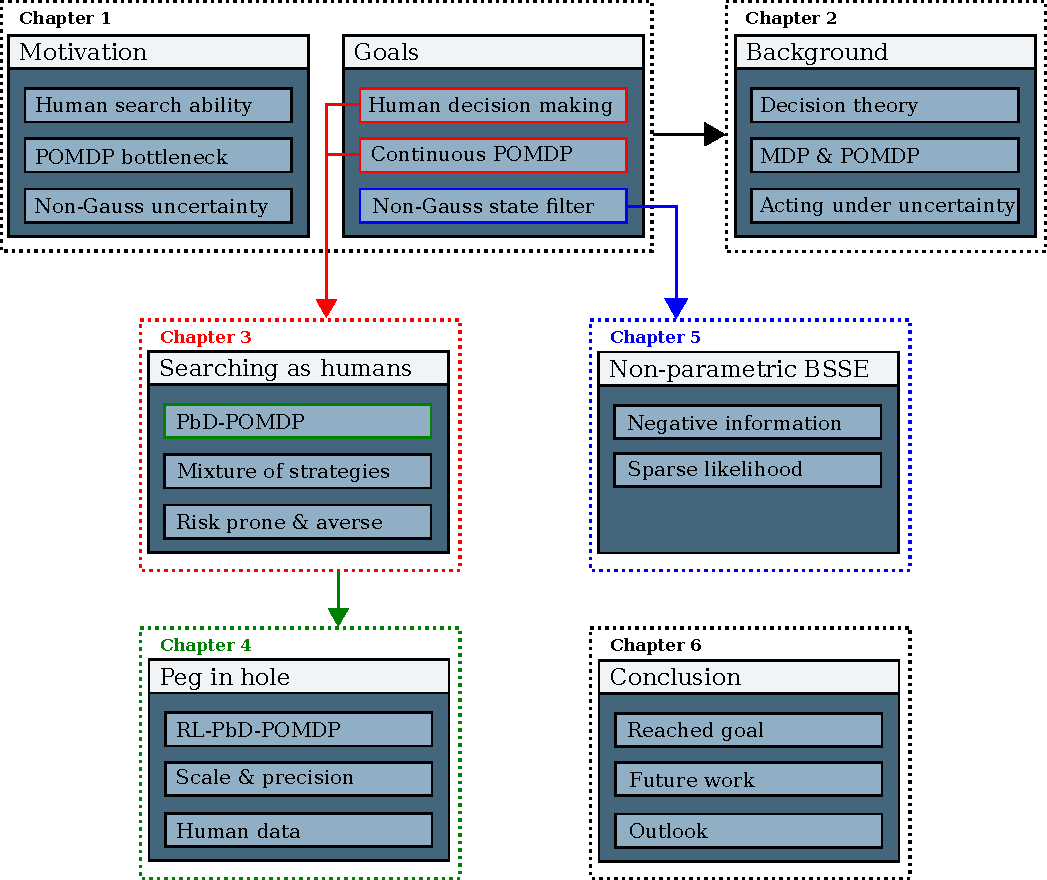
\includegraphics[width=\textwidth]{./ch1-Introduction/Figures/roadmap.pdf}
  \caption{Roadmap of the Thesis with. Three contributions are partitioned in the 3rd, 4th and 5th chapters.}
  \label{fig:rmap_thesis}
\end{figure}

\section{Thesis outline}

The thesis is structured according to three main contributions outlined in the previous section, 
each comprising a chapter and the following paragraphs give a detailed outline of the structure 
of this thesis, see Figure \ref{fig:rmap_thesis}.

\begin{minipage}[c]{0.9\textwidth}
\paragraph{Chapter 2 - Background}\\
In this chapter we introduce and mathematically formalise the sequential decision making problem 
under uncertainty and we provide a detailed literature review of the related work in this domain.
We provide a brief introduction to \textit{Decision Theory} before focusing on the work 
in AI \& robotics relevant to POMDPs whilst highlighting their relevance and contribution to our work. 
\end{minipage}

\begin{minipage}[c]{0.9\textwidth}
\paragraph{Chapter 3 - Learning to reason with uncertainty as humans}\\
In this chapter we present an approach for transferring human skills in a blind haptic 
search task to a robot in our PbD-POMDP framework. The belief of the human is represented by a particle filter and 
all subsequent beliefs are inferred from the human's motions acquired via a motion tracking
system. A generative model of the joint belief and actions distribution is learned and used
to reproduce the behaviour on a WAM and KUKA robot in two search tasks. Experimental 
evaluations showed the approach to be superior to greedy opportunistic policies and traditional
path planning algorithms. 
We also provide a review of work related to humans taking decisions under uncertainty 
in spatial navigation and haptic tasks with an emphasis on works which consider diminished or no 
visual information. This chapter has been published in \cite{deChambrierBillard2013,Chambrier2014}.
\end{minipage}

\begin{minipage}[c]{0.9\textwidth}
\paragraph{Chapter 4 - Reinforcement learning in belief space}\\

In this chapter we present a similar approach to the one in Chapter 3, ``Learning to reason with uncertainty as humans'',
with the difference that we explicitly encode the task through the introduction of a binary objective function and we consider 
a peg-in-hole task under high levels of uncertainty. 
The task requires both high and low levels of precision from the agent to be able to accomplish it, which makes it particularly interesting. 
We demonstrate the importance of initially provided human data as opposed to using data generated from a greedy policy.
We learn a value function approximation of the belief space through locally weighted regression and approximate dynamic programming. By combining a PbD approach in this Actor-critic Reinforcement Learning framework, we demonstrate an improvement upon 
a purely statistical controller with nearly no additional cost. We refer to this approach as RL-PbD-POMDP. Elements of this chapter are to appear 
in \cite{FPI_Chambrier2016}.
\end{minipage}

\begin{minipage}[c]{0.9\textwidth}
\paragraph{Chapter 5 - Non-parametric Bayesian state space filter}\\
In this chapter we present an approach to perform a state space estimation of a map and agent 
given that there is no direct observation between the landmarks and the agent. 
We demonstrate that by keeping track of the applied measurement functions rather than 
explicitly parametrizing the full joint distribution of the landmarks and agent we can fully reconstruct 
the optimal Bayesian state estimation. The advantage of our approach is that the space complexity is linear as opposed 
to exponential. We validate our approach in 2D search navigation tasks.
We also give an overview of the literature of SLAM and elucidate the position of our filter within it. This chapter 
has been submitted to \cite{MLMF_Chambrier2016} and is under review.
\end{minipage}

\begin{minipage}[c]{0.9\textwidth}
\paragraph{Chapter 6 - Conclusion}\\
We conclude by providing a holistic summary of our work and achievements. We draw attention to the current 
open problems and directions for future work in the field of uncertainty and reasoning in AI and robotics.
\end{minipage}







 	\fi
\ifdefined  	\gDisplayBackground		\chapter{Background}

% Introduce what is planning under uncertainty
Acting under uncertainty is central to AI and robotics and has been an active area of research for decades. It
is an umbrella term which encompasses a wide spectrum of fields:  \textit{economics}, \textit{psychology}, 
\textit{cognitive science}, \textit{neuroscience}, \textit{robotics} and \textit{artificial intelligence}.
The work in this thesis relies on results from all of the aforementioned fields with varying degree.
Cognitive and neuroscience bring justification and biological inspiration in the way we represent our beliefs and how we act accordingly. 
AI and robotics provide computational models and optimisation methods some of which are biologically inspired to be able to solve decision
problems given uncertainty.
Because of the vast spectrum of topics we cannot do justice to all them and we will focus on works which are directly 
relevant to the problems we are addressing in this thesis, \textit{which is how to teach a robotic apprentice to act under uncertainty}.
In this chapter we cover the following topics in the presented order: Decision Theory (DT), Markov Decision Process (MDP), 
Partially Observable Markov Decision Process (POMDP), a literature review and the approach taken 
in this thesis.\\[0.05cm]

\begin{figure}[h]
 \centering
 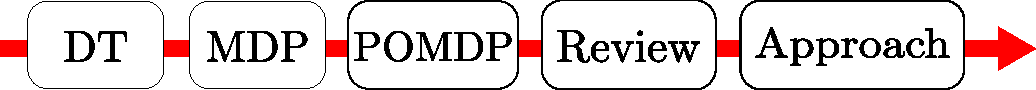
\includegraphics[width=0.9\textwidth]{./ch2-Background/Figures/chap_overview.pdf}
  \caption{Chapter outline.}
  \label{fig:ch2_outline}
\end{figure}

\begin{itemize}
 \item \textbf{Section} \ref{sec:deci_un}, introduces what is meant by taking decisions under uncertainty and what are the different 
 sources of uncertainty. We take a historical look at Decision Theory since it is the root node of all subsequent research in reasoning 
 and acting under uncertainty and provides for a good introduction to the topics which will follow.  
 \item \textbf{Section} \ref{sec:sqp},  mathematically formalises the sequential decision problem under uncertainty and is linked with Decision Theory. We derive from first principal 
 the Bellman optimal equation which is one of the most important result to date in sequential decision processes.
 \item \textbf{Section} \ref{sec:lit_rev}, provides an in depth literature review with the latest results in AI \& robotics in the subject 
of planning and acting under uncertainty. We draw attention to the different approaches to solving this problem whilst pointing out
their advantages and weaknesses. We summaries what has been achieved so fare and what are the open problems.
 \item \textbf{Section} \ref{sec:approach}, the core approach taken by this thesis is detailed. We outline how we teach a robotic apprentice 
 to act under uncertainty.
\end{itemize}



\section{Decisions under uncertainty}\label{sec:deci_un}
% What is the the reasoning under uncertainty planning problem
% What are all the assumptions which can be made regading the belief

%In this section we introduce and frame the problem we seek to solve in generic 
%terms. 
The main objective of reasoning under uncertainty is to find an action or sequence of
actions which will result in the most preferable outcome. There are two key attributes which can render this 
problem difficult: \textbf{stochastic actions} and \textbf{latent states}. 

Stochastic actions when applied in the same state will not always result in the same outcome. This type of uncertainty 
can arise from many sources. For instance, the outcome of chaotic systems will always lead to different results when the same action is applied
to the same initial conditions, such as the throwing of a dice or the flipping of a coin. In outdoor robotics the terrain might lead to slippage, causing 
the robot to skid, or in an underwater environment currents might drastically offset the position of an UAV. In articulated robots, the friction in the joints 
can result in an error in the end-effector position (especially true for cable driven robots).

The second source of uncertainty is when the state space cannot be determined. This arises when the sensors are not able to 
provide sufficient information to reliably estimate the state. In robotics this uncertainty can arise from inadequate or noisy sensors. 
In poor environmental conditions such as humidity, lack of light or smoke the robot can experience difficulties in 
ascertaining its position and thus in planning how to achieve a given objective.

Given these two types of uncertainty, the question is how to represent these uncertainties. The predominant approach 
is to quantify the uncertainty in terms of probabilities. For instance the application of a forward action to a wheeled robot 
will result in some probability in a new position further ahead and with a remaining probability distributed to adjacent 
regions which might have occurred due to slippage.

An observation made through the robot's sensors will result in a probability distribution over the robot's probable location.
This quantification of the action and observation uncertainty, in terms of a probability distribution over the state, must
be utilised by the agent to plan actions towards accomplishing its goal. In order to take a decision, the agent must assign a utility 
to each state weighted by the probability of its outcome and act so as to get the highest utility. The utility indicates a 
preference over the outcomes and when combined with probabilities leads to Decision Theory, which is the topic of the next section. 

\subsection{Decision theory}\label{sec:ch2_DT}

The central question that Decision Theory asks is: \textit{how do we take decisions when faced with uncertain outcomes ?} To answer
such a question we need to identify the attributes which are involved when we take a decision, namely our \textbf{beliefs} and 
\textbf{desires}. Beliefs reflect a degree of knowledge we have about the world. This degree is ascertained by 
the amount of evidence we have in support of our beliefs. Epistemology studies in great detail the relationship between 
truth, beliefs and knowledge. We will not go into a philosophical discussion of their interplay, but make use of the following: 
if we have sufficient evidence in support of our beliefs and they represent the truth then we consider them to 
be \textbf{rational beliefs}. As for desires, they are linked to our disposition to take upon them. For 
example if I want to switch off my alarm clock I have to look for it in the last area I believed it to be in. 
These two attributes, beliefs and desires, are used to frame a decision problem. Early work in decision theory assumed 
that the problem was well grounded and focused on finding what \textbf{rational actions} need to be taken given our beliefs 
in order to achieve our desires. 

\begin{figure}
 \centering
 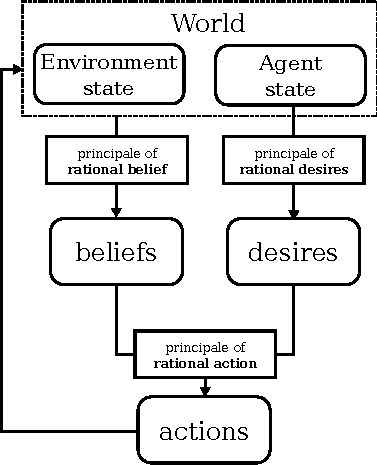
\includegraphics[width=0.5\textwidth]{/home/guillaume/Documents/Thesis/ch2-Background/Figures/cognitive_loop.pdf}
  \caption{Relation between beliefs, desires and actions and are all considered to be rational.}
\end{figure}

Early interest in such questions were typically centred around economics which included deciding an appropriate 
investment or wager for a particular gamble. It was noted that the expected monetary outcome of a gamble as a means of basing a 
decision, would often lead to a course of action which contradicts common sense. A famous example of this contradiction
is demonstrated in the St. Petersburg paradox. In this paradox a bookmaker proposes the following gamble. 
An initial pot starts with a content of \pounds2. The bookmaker proceeds to flip a fair coin until the first appearance of a 
tails which ends the game. Until the occurrence of the first tails the money in the pot doubles after every toss. Once the 
game ends the player leaves with the contents of the pot. As an avid gambler and \textbf{expected value} maximiser how much 
would one be willing to pay to enter this game ? To access, one would need to know the average payout. The amount 
of money increases by \pounds$2^{n}$, where $n$ is the number of non-final tosses and the probability of 
reaching $n$ is $1/2^{n}$. In this case the expected monetary outcome is infinite:

\begin{equation*}
\displaystyle \mathop{\mathbb{E}}_{p(\pounds)}\{\pounds\} = \underbrace{\frac{1}{2} \pounds2}_{\textrm{first toss}} + \frac{1}{4} \pounds4 + \dots = \sum\limits_{n=1}^{\infty} 
\pounds\frac{2^{n}}{2^{n}} = \pounds\infty 
\end{equation*}

So the expected gain or return for paying to enter such game is an infinite amount of money. Thus in principal if a player was
seeking to maximise his expected return value he would be willing to pay an amount close to infinity to enter the game. 
This does not seem a good decision rule; no person in the world would be willing to pay such high amounts to enter this game.

Nicolas Bernoulli proposed a solution to the problem which was later published by his brother Daniel (republished \cite{Bernoulli1954}). 
He introduced the notion of a \textbf{utility function}, and he claimed that people should base their decision on 
the expected utility instead of solely on the monetary outcome.

\begin{quote}
  \onehalfspacing% <--- Local line spacing
  ``...the value of an item must not be based on its price, but rather on the utility it yields."\par\raggedleft--- \textup{Daniel Bernoulli}
\end{quote}

The introduction of a utility function takes into account that the net worth of a person will influence their decision since 
different people (in terms of their monetary worth) will weigh the gain differently. The utility function introduced by Bernoulli 
was the logarithm of the monetary outcome $x \in X$ weighted by its probability $p(x)$ which results in an expected utility: 

\begin{equation*}\label{eq:exp_utility}
  U(x) = \displaystyle \mathop{\mathbb{E}} \{ u(x) \} = \sum_{x\in X} p(x) \underbrace{\log(x)}_{u(x)}
\end{equation*}

%Different utility functions characterise different levels of risk. When the it is concave as it for Bernoulli's utility function
%the person will be \textbf{risk-averse}, when linear \textbf{risk-neural} and convex \textbf{risk-seeking}. 
%This was the first introduction of a utility function. 

It is later in 1944 that von Neumann and Morgenstern (\cite{VonNeumann1944}) axiomised Bernoulli's utility function 
and proved that if a decision maker has a preference over a set of lotteries\footnote{the term lottery refers 
to a probability distribution in the original text.} which satisfy four axioms
(completeness, transitivity, continuity, independence) then there exists a utility function whose expectation 
preserves this preference. An agent whose decisions can be shown to maximise the vNM expected utility are said 
to be \textbf{rational} otherwise they are \textbf{irrational}.

%\begin{equation*}
% a^* = \max_a U(x|a)
%\end{equation*}


This is the theoretical basis of most economic theory. It is a \textbf{normative} model of how people should behave given uncertainty. It is also the basis of most 
if not all decision making, cogitative architectures and control policies in AI and robotics (to the best of the author's knowledge).

An aspect to keep in mind regarding the vNM model is that it is normative; it states what should be a rational decision. 
As a result it is not always consistent with human behaviour. There is great debate regarding 
the predictions made by vNM models with respect to our behaviour. There have been many studies both demonstrating divergence 
between the model's predictions and our observed behaviour but also supporting evidence that it does reflect 
the output of our decision making process. Reasons for divergence have been attributed to how people
weigh probabilities and how the decision problem is framed. But probably the most important aspect is that 
in most decisions we are faced with, the quantification and rationality of our beliefs might not be adequate
and limitations of our working memory will come into play in the final decision.

Nevertheless vNM agents are predominantly used in AI and robotics as a means of implementing 
decision making processes or in control policies. In psychology and cogitative science vNM agents
are a used for comparing human behaviour against an optimal strategy (by optimal we mean it is rational in 
the vNM sense). It is important to remember the origins and assumptions underlying the models that 
are used to represent control policies or cognitive architectures implemented into robotic systems or 
software agents.

% (see prescriptive models(\cite{Kahneman79prospecttheory}). 
% vNM is concerned with a one shot only decision, but what if we have to take a sequence of decisions ? What 
% happens then ?
% How is the uncertainty quantified ? Answer: probability theory
% How does the agent make a decision ? He must assigned a preference to the outcome of various actions
% Utility theory and combined with probability lead to decision theory.
% Speak about the historical context of plannig un
% Uncertainty and rational actions
% vNM theorem is limited to evaluation options that come with an 
% objective probability distribution over outcomes.
% a situation decision theoriests and economists often describe 
% as ''choice under risk``
% The utility function represents the agents desires.
% so the probability function represents her beliefs.
% The theories are referred to collectively as subjective expected utility (SEU).
% How is decision theory used in robotics ?
% POMDPs provide a rich framework for sequential decision-making under uncertainty in stochastic domains.
% Solving a POMDP is often intractable.

\begin{table}
\begin{center}
\renewcommand{\arraystretch}{1.5}
\begin{tabular}{|l|p{9cm}|} 
\hline
    \textbf{Notation} 			 	& \textbf{Definitions} \\ \hline\hline
    $x_t \in \mathbb{R}^3$ 		 	& Cartesian state space position of the agent end-effector.\\
    $y_t \in \mathbb{R}^{M}$		 	& Observation/measurement from the agents sensors.\\
    $a_t \in \mathbb{R}^3$		 	& Action, Cartesian velocity of the end-effector of the agent.\\
    $X,Y,A$				 	& State, observation and action random variables where $x$, $y$ and $a$ are realisation.\\
    $p(x_t)$ 					& Short hand notation for a probability density function, $p_{X}(x_t)$.\\
    $x_{0:t}$					& $\{x_0,x_1,\cdots,x_{t-1},x_t\}$, history up to time $t$.\\
    $p(x_t|y_{0:t},a_{1:t})$	 		& Filtered probability distribution over the state space given the action and observation history.\\
    $b_t$					& Belief state is the filtered state space distribution
						 $b_t = p(x_t|y_{0:t},a_{1:t})$ which will be written as $b_t$ for simplicity.\\
    $\policy(a_t|\cdot)$ 			& Parametric probabilistic policy, $a_t \sim \pi_{\boldsymbol{\theta}}(a_t|\cdot)$, where $\boldsymbol{\theta}$ is the parameters.\\
    $u(x) \in \mathbb{R}$			& Utility function, returns the utility of being in state $x$. It can also be dependent on the action, $u(x,a)$.\\
    $\gamma \in [0,1)$				& Discount factor, the closer to one the more the later utilities are considered. When set to zero, only immediate utilities are 
						  considered which would result in a myopic greedy agent.\\
    $p(x_{t+1}|x_t,a_t)$			& State transition model, returns the likelihood/probability of reaching state $x_{t+1}$ given that action $a_t$ is applied in state $x_t$.\\	
    $p(y_t|x_t)$				& Observation/measurement model, returns the likelihood/probability of observing $y_t$ given that the agent is in state $x_t$.\\
    $\tau(b_{t},u_{t},y_t)$		& Updates a belief given a motion and observation. It makes use of both the motion and observation functions. The state space estimation function, $\tau$, can be any kind of state space filter such as an Extended Kalman Filter (EKF) or a Particle Filter (PF).
    \\ \hline
\end{tabular}
\end{center}
\caption{Definition of common variables used.}
\label{tab:notation}
\end{table}


\section{Sequential decision making}\label{sec:sqp}

When Decision Theory is brought up, we are usually referring to a one shot non-temporal decision. 
However many interesting decision problems are sequential. In such situations, we must consider 
the effect current decisions will have on future decisions. Expected utility theory (part of Decision Theory) is 
extendable to a temporal decision problem. There are however two subtle but important 
differences between the temporal and non-temporal decision problems. The first difference is the utility. In the one 
time step problem an outcome has one utility assigned to it, $u(x)$. In the temporal decision problem a utility has to 
be assigned to a sequence of outcomes, $u(x_{0:T})$, where $T$ is the number of sequential decisions taken. The utility 
of a sequence is the sum of the individual utilities. However if the decision problem is 
non terminating this will lead to an unbounded utility. To bound the utility a discount factor $\gamma \in [0,1)$ is 
introduced and the new temporal utility function becomes:

\begin{equation}
    u(x_{0:T}) 	   := \sum\limits_{t=0}^{T} \gamma^{t} u(x_t) \label{eq:joint_state_actions_util}
\end{equation}

The discount factor controls the importance that later utilities have on the final utility. If the discount factor is set to
zero we obtain the original one shot utility function and if we were to take actions which maximised the expected utility 
we would not be considering at all the effect current decisions have at future decision points. An agent reasoning in such a way is 
called \textbf{myopic}.
The second difference between the temporal and non-temporal decision problem is the way in which probabilities are assigned to 
outcomes. This was $p(x)$ in the Decision Theory utility function formulation.
Now because of the sequential nature of the problem we consider a conditional state transfer probability distribution $p(x_{t+1}|x_t,a_t)$
which models the probability of going from state $x_t$ to $x_{t+1}$ given that action $a_t$ is taken. This particular representation of a
sequential decision problem is called a \textbf{Markov Decision Process (MDP)} and to be more exact a first order MDP.
The necessary models are the state transition and utility functions. The assumption of such a model is that all necessary information to 
take a decision is encoded in the current state and there is no need to consider the history of state transitions when taking a current decision.
In Figure \ref{fig:mdp} we illustrate two graphical representations of a MDP, which are known as \textbf{Dynamic Bayesian Networks (DBN)}.
A DBN represents the temporal relationship and conditional dependence between random variables, decisions and utilities, which are 
represented by circles, squares and diamonds. For the MDP to the left the actions are not stochastic, whilst for the MDP on the right 
the actions taken are governed by a stochastic \textbf{policy}, $\policy(a_t|x_t)$. A policy represents the plan of an agent for each state,
given a state it will output an action. A policy is considered optimal when it maximises the expected utility function, it is optimal in the vNM sense.

\begin{figure}[h]
  \centering
  \subfigure[off-policy]{\label{fig:mdp_off}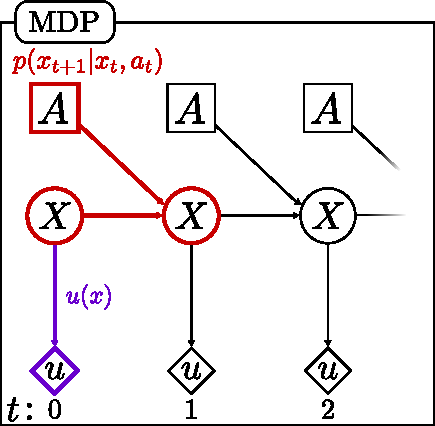
\includegraphics[width=0.45\textwidth]{/home/guillaume/Documents/Thesis/ch2-Background/Figures/mdp3.pdf}}
  \subfigure[on-policy]{\label{fig:mdp_on}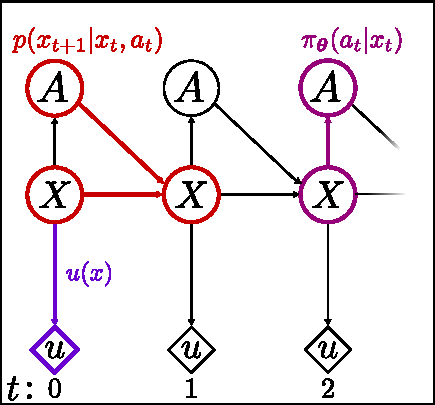
\includegraphics[width=0.45\textwidth]{/home/guillaume/Documents/Thesis/ch2-Background/Figures/mdp2.pdf}} 
  \caption{Dynamical Bayesian Network of a Markov Decision Process; it encodes the temporal relation between the random variables (circles),
  utilities (diamond) and decisions (squares). The arrows specify conditional distributions. In \textbf{(a)} the decision nodes are not considered 
  random variables whilst in \textbf{(b)} they are. From these two DBN  we can read off two conditional distributions, the state transition distribution (in red) and the action distribution (in purple). }
    \label{fig:mdp}
\end{figure}

Solving a MDP means finding a policy whose actions in any given state will always maximise the expected utility. Such 
a policy is usually denoted as $\pi^*$, the \textbf{optimal policy}. As in decision theory, the expected utility is the utility 
of  a sequence of states $u(x_{0:T})$ weighted by its probability. The graphical representation (Figure \ref{fig:mdp} (a)) allows 
the probability of a sequence of states and actions, to be read off directly: 
\begin{align}\label{eq:joint_state_actions}
  p(x_{0:T},a_{0:T-1}) &= p(x_{0}) \prod_{t=0}^{T-1} p(x_{t+1}|x_t,a_t) \\
  u(x_{0:T}) 	       &= u(x_0) + \gamma u(x_1) + \dots + \gamma^{T-1} u(x_{T-1})  + \gamma^T u(x_T)
\end{align}
We are interested in finding the sequence of actions, $a_{0:T}$, which will maximise the expected utility function:
\begin{equation}\label{eq:temporal_expected_utility}
 \argmax_{a_{0:T-1}} U(x_{0:T},a_{0:T-1}) = \max_{a_0} \sum\limits_{x_1}   \cdots  \max_{a_{T-1}} \sum\limits_{x_T} \Bigg( p(x_{0:T},a_{0:T-1}) u(x_{0:T}) \Bigg)
\end{equation}
Solving the above directly in its current form would to lead to an exponential complexity. Making use of the first order 
Markov assumption and that current utilities do not depend on future utilities, the summations can be re-arranged and 
a recursive pattern emerges which can be exploited: %which results in Equation \ref{eq:expansion}
\begin{align}\label{eq:expansion}
 &\argmax_{a_{0:T-1}} U(x_{0:T},a_{0:T-1}) =\max_{a_0} \sum\limits_{x_1}   \cdots  \max_{a_{T-2}} \sum\limits_{x_{T-1}} p(x_{0:T-1},a_{0:T-2})  \nonumber\\
 &\left( u(x_{0:T-2}) + \gamma^{T-1} \left( u(x_{T-1}) +  \gamma \max_{a_{T-1}} \sum\limits_{x_{T}} p(x_{T}|x_{T-1},a_{T-1}) u(x_{T}) \right) \right)
\end{align}
From the rearrangement we notice that Equation \ref{eq:expansion} has the same functional form as Equation \ref{eq:temporal_expected_utility}, 
except that the recursive component can be summarised by Equation \ref{eq:bellman}, which is known as 
the \textbf{Bellman} optimal equation (the asterisk indicating that it is optimal),
\begin{equation}\label{eq:bellman}
 V^*(x_t) := u(x_t) + \gamma \max_{a_t} \sum\limits_{x_{t+1}} p(x_{t+1}|x_t,a_t) V(x_{t+1})
\end{equation}
where for the terminal state $V_T(x_T) = u(x_T)$. The Bellman equation is a means of solving a sequential decision problem 
through use of dynamic programming. It shows that the utility of the current state is based on the immediate utility and 
the discounted maximum utility of the next state. Making use of this recursion reduces the computation complexity which is now 
quadratic in the number of states, $\BigO(T\, |A|\, |X|^2)$. To find the optimal value and subsequent policy an approach 
would be to repeatedly apply the Bellman equation to each state until the value function converges. What makes the problem 
difficult to solve is maximisation over the actions. This induces two problems, the first is that the optimisation is nonlinear 
and the second is that if the action space is continuous the maximisation will be expensive to compute.
This brings into play the two main approaches to solving a MDP: \textbf{off-policy} and \textbf{on-policy}.
Off-policy methods solve directly for the optimal value function, $V^*(x)$, and perform the maximisation over the actions. \textbf{Value-Iteration (VI)}
is such a method. On-policy approaches, $V^{\pi}(x)$, find the optimal value and policy through repeating \textbf{policy evaluation} and
\textbf{improvement} steps. In the policy evaluation the value or utility of a policy is found through solving the on-policy version of the Bellman 
equation:
\begin{equation}\label{eq:on_policy_bellman}
  V^{\pi}(x_t) := u(x_t) + \gamma \sum\limits_{a_t} \policy(a_t|x_t) \sum\limits_{x_{t+1}} p(x_{t+1}|x_t,a_t) V(x_{t+1})
\end{equation}
In the policy improvement step, the policy is made more greedy by maximising the value function. Through the repetition of these two 
steps both the value function and policy converge to the optimal. On-policy methods are preferred in settings where the action 
space is highly continuous, such as in robotics. Using dynamic programming is however not the method of choice since it requires 
multiple passes through the entire state space and for this reason it is necessary to have the model of the state transition a priori. 
Instead \textbf{Reinforcement Learning (RL)} methods are used to find an optimal value and policy. RL is a sample based approach
in which an agent interacts with the environment gathering examples of state transitions and the utility and uses them 
to gradually solve the Bellman equation.

We introduced the formulation of a sequential decision process for the MDP model and showed how an optimal policy 
and value function are obtained through maximising the expected utility. The re-arrangement of the summations, known as
variable elimination, allows to exploits a recursive structure present in the Markov chain. The recursive component 
turns out to be the Bellman optimal equation, which when solved (via dynamic programming or reinforcement learning) results 
in an optimal value and policy function. A MDP models the uncertainty inherent in the state transition but not the uncertainty 
of the state. The MDP assumes that the state space is always fully observable, which is a strong assumption. In robotics, the 
on board sensors return an estimate of the state with a certain amount of uncertainty associated with it. To take this additional
uncertainty into consideration the MDP has to accommodate it. This leads to a Partially Observable Markov Decision Process (POMDP).





% Define box and box title style
\tikzstyle{white_box}  = [draw=black, fill=white, very thick,  rectangle, rounded corners, inner sep=10pt, inner ysep=20pt]
\tikzstyle{fancytitle} = [fill=white,draw= black, text=white,rounded corners=1mm,text=black]


\subsection{POMDP}
%\begin{equation}
% y_t =  \begin{bmatrix}
%       r    \\
%       \phi \\
%     \end{bmatrix} \in \mathbb{R}^2
%\end{equation}

A POMDP is a popular approach for formulating a sequential decision process in which both motion and observation 
uncertainty are considered. In this partially observable setting the agent does not know with exactitude the state of the environment,
but is able to observe it through his \textbf{sensors}. We define a sensor mathematically as being a function of the 
state space, $x_t$, relating to an observation, $y_t$, corrupted by some noise, $\epsilon_t$,

\begin{equation}\label{eq:sensor}
  y_t = h(x_t) + \epsilon_t
\end{equation}

The sensor function $h(x_t)$ can be linear or non-linear and the additive noise term $\epsilon_t$ can 
be Gaussian (usually the case), non-Gaussian, state dependent or not. The uncertainty of the latent state, $x_t$, is quantified by a probability distribution, $p(x)$. 
This probability distribution represents all the hypothetical positions in the world in which the agent can be found. In Figure \ref{fig:belief_update_example} \textbf{(a)} an agent is located in a square yard 
containing a wall. Initially the agent is confident of his position; his state uncertainty $p(x_0)$ is low, represented 
by the blue probability density. However during a circular displacement the agent skids and the state uncertainty is increased 
by the state transition function, $p(x_{t+1}|x_t,a_t)$; this step is referred to as \textbf{motion update}. To reduce the uncertainty, the agent takes a measurement, $y_t$, with 
his sensors which provide range, $r$, and bearing, $\phi$, information with respect to the wall, see Figure \ref{fig:belief_update_example} \textbf{(b)}.
The agent uses the model of his sensor, known a priori, to deduce all possible locations in the world from where the current 
measurement could have originated. This model is known as the measurement likelihood function: 
\begin{equation}\label{eq:likelihood}
 p(y_t|x_t) = \mathcal{N}(y_t - h(x_t);0,\Sigma)
\end{equation}
The measurement likelihood function makes use of the measurement function $h(x)$ and it models the noise 
in the sensor. In this case the noise model, $\epsilon_t$, is Gaussian, paramaterized with mean zero and covariance $\Sigma$.
Typically the parameters of the measurement likelihood function are learned a priori.

\begin{figure}
  \centering
  \subfigure[]{\label{fig:motion_update}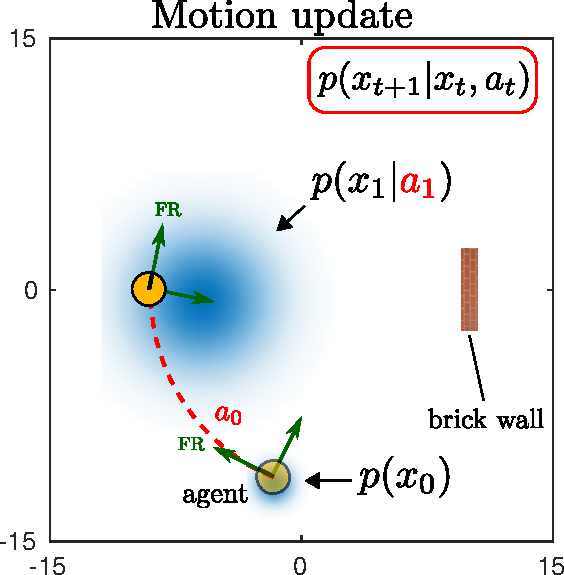
\includegraphics[width=0.45\textwidth]{/home/guillaume/Documents/Thesis/ch2-Background/Figures/motion_update.pdf}}
  \subfigure[]{\label{fig:measurement}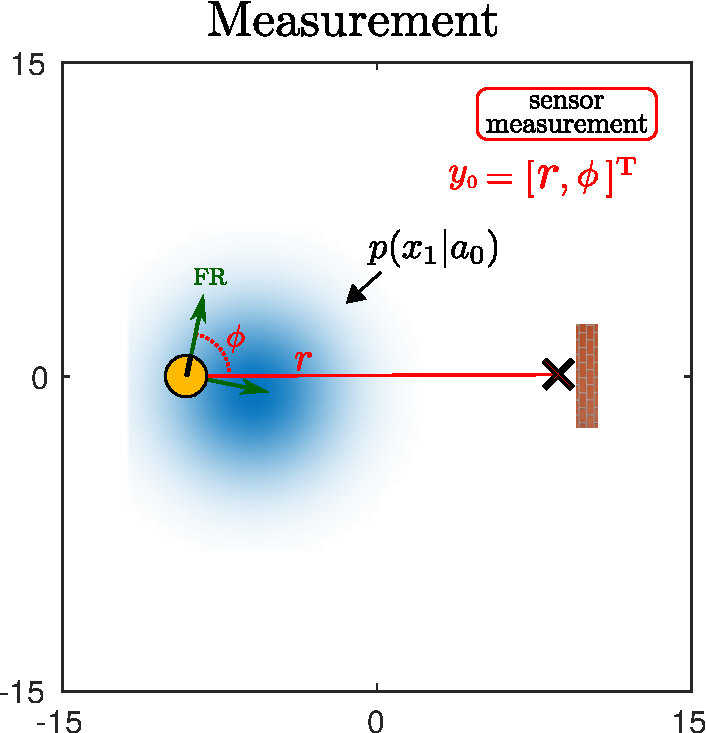
\includegraphics[width=0.45\textwidth]{/home/guillaume/Documents/Thesis/ch2-Background/Figures/measurement.pdf}} 
  \subfigure[]{\label{fig:likelihood}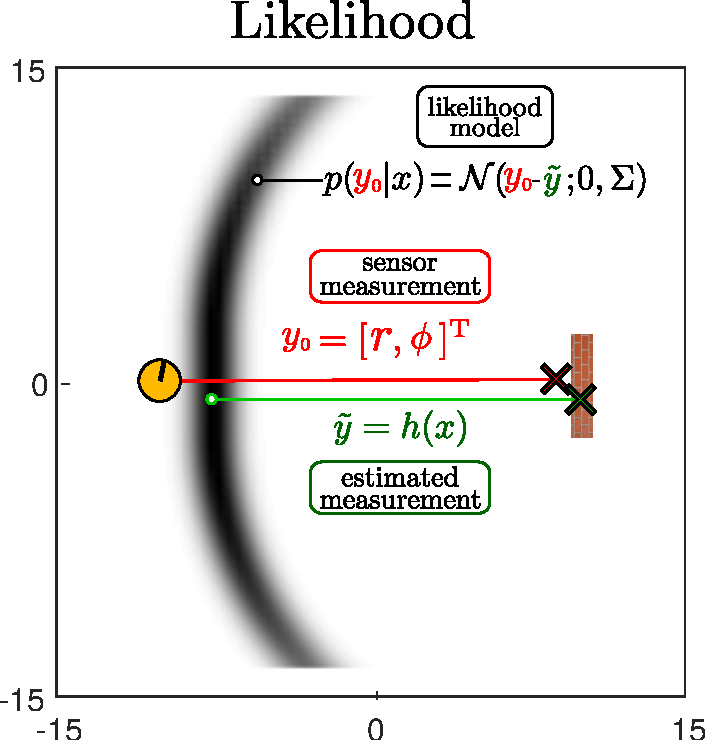
\includegraphics[width=0.45\textwidth]{/home/guillaume/Documents/Thesis/ch2-Background/Figures/likelihood.pdf}} 
  \subfigure[]{\label{fig:measurement_update}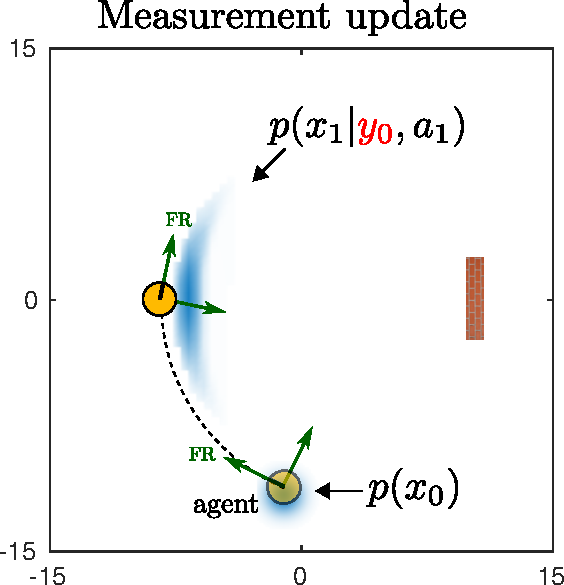
\includegraphics[width=0.45\textwidth]{/home/guillaume/Documents/Thesis/ch2-Background/Figures/measurement_update_v2.pdf}} 
 \caption{\textbf{(a)} An agent is located to the south west of a brick wall. It is equipped with a 
  range sensor. The agent takes a forward action but skids, which results in a high increase of the uncertainty.\textbf{(b)} 
  The agent takes a measurement, $y_0$, of this distance to the wall; because his sensor is noisy his estimate is inaccurate. 
  \textbf{(c)} The agent uses his measurement model to evaluate the plausibility of all locations in the world which would result in a similar
  measurement; illustrated by the likelihood function $p(y_0|x_0)$. \textbf{(d)} The likelihood is integrated into the probability 
  density function; $p(x_0|y_0) \propto p(y_0|x)p(x_0)$.}
  \label{fig:belief_update_example}
\end{figure}

In Figure \ref{fig:belief_update_example} \textbf{(c)} the likelihood is illustrated. The dark regions indicate areas of high 
likelihood, which are possible locations from which the sensor measurement could have originated. The value of the measurement
likelihood function is then integrated into the state space probability density function; this step is referred to as \textbf{measurement update}.

The two update steps, motion and measurement, are part of a recursive state estimation process called a \textbf{Bayesian state space filter}, 
which we formalise below in Equation \ref{eq:motion_update}-\ref{eq:measurement_update}.
\begin{figure}
\centering
\begin{tikzpicture}    
\node [white_box] (box){%
     \begin{minipage}{0.9\textwidth}
     The Bayesian filter turns a prior probability distribution over the state space, $p(x_{t-1}|y_{0:t-1},a_{1:t-1})$,
  to a posterior $p(x_t|y_{0:t},a_{1:t})$ by incorporating both motion and measurement. Applied recursively it 
  keep a probability distribution over the state space which considers all the past history of actions and observations. We define 
  the application of these two steps by the filter function $\tau$, which takes the current belief, the applied action 
  and measurement, and outputs the next belief, $b_{t+1}$.\\
  
  \textbf{Motion update}
	\begin{equation}\label{eq:motion_update}
	  p(x_t|y_{0:t-1},a_{1:t}) = \int p(x_t|x_{t-1},a_t)\, p(x_{t-1}|y_{0:t-1},a_{1:t-1})\;dx_{t-1}
	\end{equation}
      \textbf{Measurement update}
	\begin{align}\label{eq:measurement_update}
	  p(x_t|y_{0:t},a_{1:t})   &= \frac{1}{p(y_t|y_{0:t-1},a_{1:t})}p(y_t|x_t)\,p(x_t|y_{0:t-1},a_{1:t}) \\
	  p(y_t|y_{0:t-1},a_{1:t}) &= \int p(y_t|x_t)\,p(x_t|y_{0:t-1},a_{1:t}) dx_t
	\end{align}   
	\textbf{Filter function}\\
	\begin{equation}
	  b_{t+1} := \tau(b_t,a_t,y_t) 
	\end{equation}
    \end{minipage}
};
\node[fancytitle, right=10pt] at (box.north west) {Bayesian filter};
\end{tikzpicture}%
\caption{Bayesian state space filter.}
 \label{fig:baysian_filter}
\end{figure}

The motion model, Equation \ref{eq:motion_update}, updates the position of the probability distribution according to 
the applied action, $a_t$, and adds uncertainty by increasing the spread of the distribution. The measurement information is 
then incorporated by Equation \ref{eq:measurement_update}. The measurement likelihood always reduces the uncertainty 
or leaves it constant. The Bayesian state space filter is such an important 
component to belief space decision making that we define it by the filter function, $\tau(b_t,a_t,y_t)$, which 
takes as input the current belief, applied action and sensed measurement and returns the resulting belief $b_{t+1}$.
The state space filter is an essential component to a POMDP which will become apparent later.

%Depending on the type of sensors: stereo cameras, infra red sensors, Kinect, 
%omnidirectional camera, etc.., there is uncertainty associated with it. It is thus important 
With the latent state, its relation to the observation variable and the Bayesian filter defined, we can introduce the POMDP model
in Figure \ref{fig:pomdp} (\textit{left}). It has the same Markov chain structure as the MDP, introduced in the previous section, but the state space $X$ is latent and 
a new layer of observation variables $Y$ is added. 

\begin{figure}
 \centering
  \centering
  \subfigure[]{\label{fig:sub_pomdp}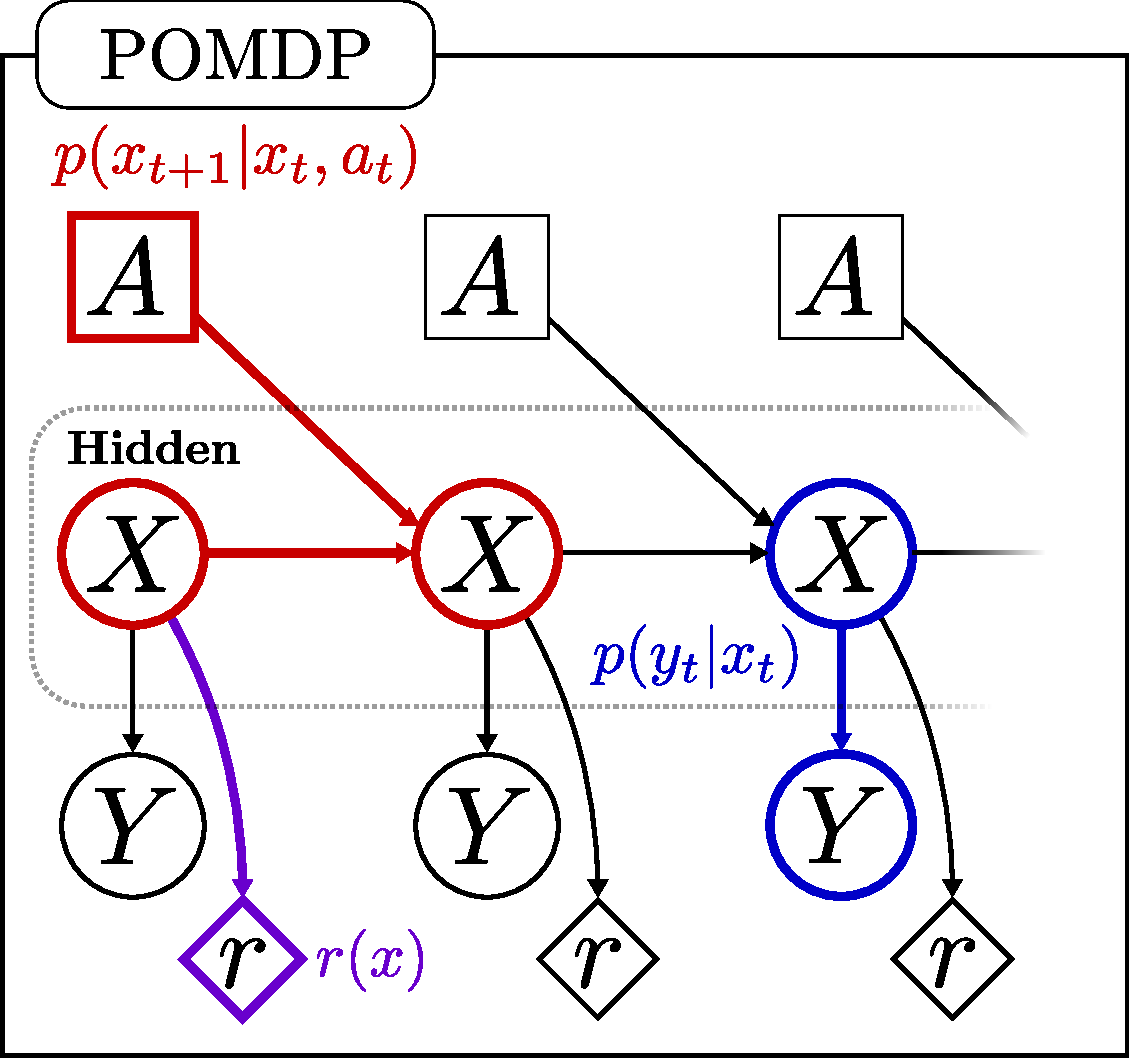
\includegraphics[width=0.45\textwidth]{/home/guillaume/Documents/Thesis/ch2-Background/Figures/pomdp2.pdf}}
  \subfigure[]{\label{fig:sub_bmdp}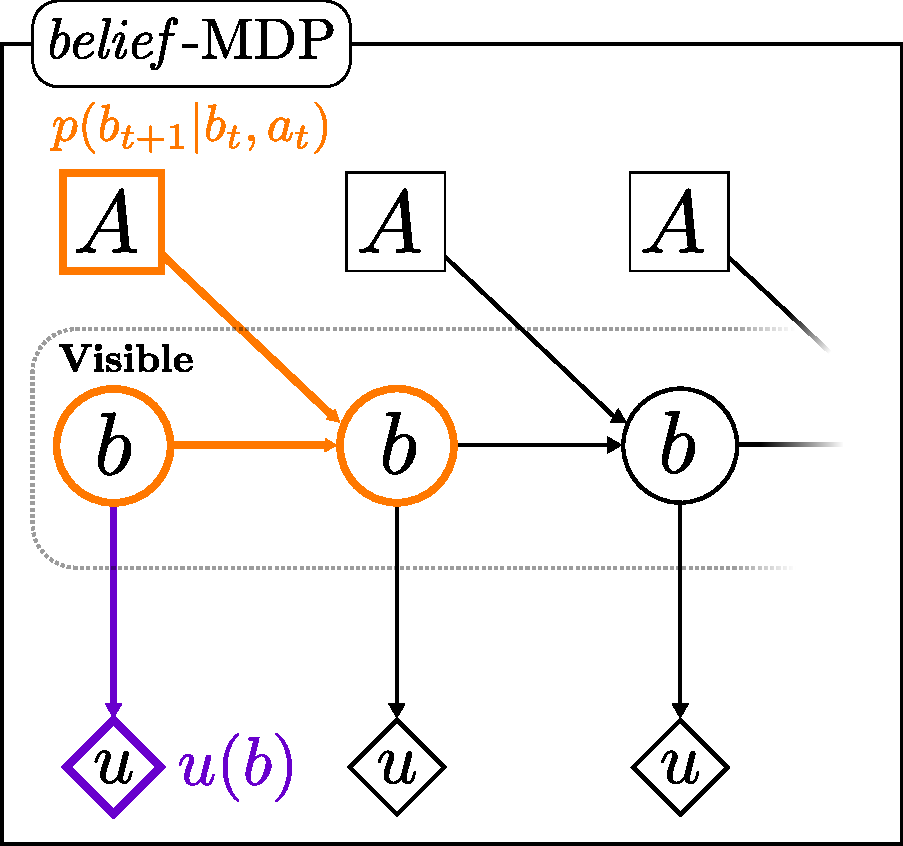
\includegraphics[width=0.45\textwidth]{/home/guillaume/Documents/Thesis/ch2-Background/Figures/pomdp3.pdf}} 
  \caption{\textbf{(a)} POMDP graphical model. The state space, $X$, is hidden, but is still partially observable through a 
  measurement, $Y$. \textbf{(b)} The POMDP is cast into a belief Markov Decision Process, belief-MDP. The state space is 
  a probability distribution, $b(x_t) = p(x_t)$, (known as a belief state) and is no longer considered a latent state. The original state 
  transition function $p(x_{t+1}|x_t,a_t)$ is replaced by a belief state transition, $p(b_{t+1}|b_t,a_t)$. The reward 
  is now a function of the belief.}
  \label{fig:pomdp}
\end{figure}

%We will see that because the state space is hidden it will cause complications to the maximisation of the expected utility.
%Since the states are not observable, the agent cannot choose its actions based on the state. The explicit 
%representation of the past events is typically memory expensive. Instead it is possible to summarize all relevant %
%information from previous actions and observations in a probability distribution over the state space, known as the
%belief state. 

As the state space is only partially observable the expected utility has to be computed for each possible history of states, actions and observations.
All approaches in the literature instead encapsulate all these possible histories into a belief state $b(x_t)$ (for short notation $b_t$)
which is a probability distribution (also referred to as an information state, \textit{I}-state) over the state 
space $x_t$ and use this new state description to cast the POMDP into a \textbf{belief-MDP} (states are probability distributions, 
beliefs). By casting a POMDP into a \textit{belief}-MDP the state space is considered observable and we recover the same structure 
as in the standard MDP problem.

As we are working within a belief space the reward function has to be adapted to:
\begin{equation}
  u(b_t) = \sum_{x_t} u(x_t)\, b(x_t) = \mathbb{E}_{b_t}\{u(x_t)\}
\end{equation}
which is an expectation. The goal as before is to find a sequence of actions 
which will maximise the expected utility. Since our \textit{belief}-MDP has the same structural form as the MDP, the solution 
to the problem is the same Bellman equation derived previously. We just substitute the new belief transition function 
and we get the corresponding belief Bellman Equation, \ref{eq:belief_bellman}.
\begin{equation}\label{eq:belief_bellman}
 V^*(b_t) = u(b_t) + \gamma \max_{a_t} \sum_{b_{t+1}} p(b_{t+1}|b_t,a_t)\,V^*(b_{t+1})
\end{equation}
However, using this equation in this form is problematic, as we are summing over the space of beliefs (which is high dimensional 
and infinite for the continuous case) and the transition function is a probability distribution over beliefs. 
The key to overcome this problem is to realise that if we know what the current measurement and applied action are, 
there is only one valid possible belief, $b_{t+1}$, and
the summation over beliefs vanishes. This can be seen by substituting the belief transition function,
Equation \ref{eq:belief_state_transformation}, into the Bellman equation Equation \ref{eq:belief_bellman}.
\begin{equation}\label{eq:belief_state_transformation}
 p(b_{t+1}|b_t,a_t) = \sum_{y_t} p(b_{t+1}|b_t,a_t,y_t)\,p(y_t|y_{0:t-1},a_{0:t})
\end{equation}
After the substitution and re-arrangement of the summation we get Equation \ref{eq:max_component}. 
Since the observation is known (because the outer summation is over $y_t$), the summation over the beliefs vanishes since there is only one possible future belief which is given by the 
Bayesian filter function $b_{t+1} = \tau(b_t,a_t,y_t)$,
\begin{equation}\label{eq:max_component}
u(b_t) + \gamma \max_{a_t} \sum_{y_t} \underbrace{\left( \sum_{b_{t+1}} p(b_{t+1}|b_t,a_t,y_t)\,V^*(b_{t+1})\right)}_{1 \cdot V^*(\tau(b_t,a_t,y_t))}\, p(y_t|y_{0:t-1},a_{0:t})
\end{equation}
which simplifies to:
\begin{align}\label{eq:final_belief_bellman}
  V^*(b_t) &= u(b_t) + \gamma \max_{a_t} \sum_{y_t}  p(y_t|y_{0:t-1},a_{0:t}) \,V^*(\tau(b_t,a_t,y_t))\nonumber  \\ 
	   &= u(b_t) + \gamma \max_{a_t} \displaystyle \mathop{\mathbb{E}}_{y_t}\{V^*(b_{t+1})\}
\end{align}

The belief Bellman equation is intuitive. The value of the current belief is the immediate utility plus the value of the 
future belief states weighted by the probability of a measurement which would result in these future belief states. 
An exact solution exists only when considering a finite state, action and observation space and a finite planning horizon $T$, \cite{Sondik_1973}.
The belief-MDP can be solved with value iteration but each backup operation (application of the bellman equation) 
results in an exponential growth in the number of parameters needed to represent the value function, which 
is computationally intractable.

Most early techniques for solving POMDPs used value iteration. The preference for persisting in doing this, given the computational
burden, is that since the utility function uses a linear operator (the expectation) and that the Bellman backup operation 
(applying the Bellman equation to the current value function) preservers the linearity, the value function after each 
updates is Piece Wise Linear and Convex (PWLC). A good text on the implementation of exact value iteration for POMDPs can be 
found in \cite[Chap. 15]{Thrun_2005} and \cite{Kaelbling_1998}.

In summary there are two problems in solving a POMDP:
\begin{itemize}
 \item \textbf{curse of dimensionality}: A discrete state space of size $N$ will result in a belief space of dimension $N-1$. The discretization
 choice will greatly impact the computational cost of Value Iteration.
 \item \textbf{curse of history}: The space and computational complexity in the worst case is exponential with respect to the planning 
 horizon, $T$, \cite{POMDP_approach_2010}.
\end{itemize}

Given such complexity it is hard to see POMDPs being actually usable for real world scenarios. As a result many approximate 
techniques have emerged with some being very successful. In the next section, we survey the literature 
and the developments of approximate POMDP algorithms and their applications.

%P-SPACE \cite{psace_mdp_1987} complete

%Before this point and before only value iteration on this subset instead of considering all beliefs.  If you have a $10 \times 10$ gird, this results in a total of a $100$ states %and a belief state of a $100$ dimensions! The PBVI approach initiated a renewed effort in 
%porting VI to POMDPs with larger and larger state spaces

%It turns out that computing a value function using the above bellman function is not computationally tractable.

%Solving 
%a POMDP problem as for the MDP case consists of finding the optimal value function from which the optimal policy can 
%b%e derived. Essentially the same dynamic programming and reinforcement learning techniques can be applied to solve 

%From considering the decision belief tree of the POMDP, Figure \ref{fig:pomdp_bel_tree}, we can appreciate the complexity of the problem
%of finding an optimal policy. Given a discrete set of actions and observations to update the belief $b_1$ we have to consider a time 
%complexity of $\mathcal{O}(|U||Y|^T)$ where $T$ is the depth of the tree (the planning horizon). Given that we have a finite set of 
%belief the complexity solving the POMDP is $\mathcal{O}(|\mathcal{B}||U||Y|^T)$. 

% In the worst cast, the exact value update procedure could require time doubly exponential in the planning horizon, T.
%Why is POMDP so good: combine information gathering and goal directed actions in one. Give taxonomy of planning under uncertainty here.

\section{Literature review}\label{sec:lit_rev}

We review the latest methods on \textit{Acting under uncertainty}. This is an extremely dense and spread out area of research, 
no doubt because of its importance. If uncertainty is not considered adequately, the control policy risks being suboptimal or lead to drastic failure. 
We will focus the review four subsections in the following order: 

\begin{itemize}
 \item \ref{lit:VI} 		\hyperref[lit:VI]{Value Iteration (VI)}
 \item \ref{lit:policy_search}  \hyperref[lit:policy_search]{Policy Search}
 \item \ref{lit:Planning} 	\hyperref[lit:Planning]{Planning}
 \item \ref{lit:heuristics} 	\hyperref[lit:heuristics]{Heuristics}
\end{itemize}

with an emphasis on robotic applications. In Figure \ref{fig:mindmap} we illustrate graphically these four topics which their associated sub-fields.

\begin{figure} 
\centering
\hspace*{-4cm}
\begin{minipage}{\linewidth}
\begin{tikzpicture}[every annotation/.style = {draw, fill = white, font = \Large}]

\path[mindmap,concept color=black!40,text=white, every node/.style={concept,circular drop shadow},  
    root/.style    = {concept color=black!40,font=\Large\bfseries},
    level 1 concept/.append style={level distance=15em,sibling angle=90,font=\large\bfseries},
    level 2 concept/.append style={level distance=9em,font=\bfseries},
  ]
    node[root] at (0,0)  {Acting under uncertainty}[clockwise from=135]
    child [concept color=red!90]  { node [concept] (PolicySearch) {Policy search} [clockwise from=180]
          child { node (EM) {EM} }
	  child { node (Gradient) {Gradient} }
	  child { node (GradientFree) {Gradient free}
        }
    }
    child [concept color=teal!90] { node {Planning}[clockwise from=50]
        child { node (BRM) {Belief\\ road maps}}
        child { node (OptimalControl) {Optimal control}}
    }
    child [concept color=orange!90] { node {Heuristics}[clockwise from=-10]
        child { node {Info.\\Gain}}
        child { node {QMDP}}
        child { node {Myopic}}
    }
    child [concept color=blue!90] { node  [concept] (ValueIteration) {Value Iteration}  [clockwise from=-55]
	child { node (Latent) {Latent\\ VI}}
        child { node (ApproxVI) {Approx. VI}}
        child { node (PBVI) {Point-base\\ VI}
        }
    };
    
    \begin{scope}[mindmap]
      \node[fill={green!40!black},circle,level 1,color=green!40!black,text=white,font=\large\bfseries] (ActorCritic) at (-5,0) {Actor-critic};
    \end{scope}
  
    \path (ActorCritic) to[circle connection bar switch color=from (green!40!black) to (blue!90)] (ValueIteration) ;
    \path (ActorCritic) to[circle connection bar switch color=from (green!40!black) to (red!90)] (PolicySearch) ;
  
    \info[7]{Latent.south}{below,anchor=north}{
      \item E-PCA
    }
    
    \info[9]{ApproxVI.south}{below,anchor=north}{
      \item MC-POMDP
    }
    
    \info[9]{PBVI.south west}{below,anchor=north}{
      \item SARSOP
      \item HSVI2
    }
  
    \info[7]{EM.south west}{below,anchor=north}{
      \item PoWER
    }
  
    \info[10]{Gradient.north west}{above,anchor=north,yshift=1cm}{
      \item REINFORCE
    }

    \info[6]{ActorCritic.south west}{below,anchor=south,xshift=-1.5cm,yshift=0.5cm}{
      \item eNAC
    }
    
    \info[9]{OptimalControl.south}{below,anchor=north}{
      \item B-LQR
      \item LQG-MP
    }
    
    \info[9]{BRM.north}{below,anchor=north,yshift=1.3cm}{
      \item BRM
      \item FIRM
    }
\end{tikzpicture}
\end{minipage}
\caption{Mind-map of AI and robotic methods for acting under uncertainty.}
\label{fig:mindmap}
\end{figure}
	
% Vision and range sensors can estimate the pose of an object, but there is still residual uncertainty.
% Tactile sensing, combined with proprioception, can give highly reliable inforation about object position.
% Uncertainty due to sensor noise is particularly problematic for fine manipulation tasks[1], such as grasping 
% and pushing a small button on a drill, hookoing the figuers of a hand around a small button on a drill.

\subsection{Value Iteration}\label{lit:VI}

The POMDP formulation introduced previously is the main theoretical starting point of policies which
consider uncertainty optimally. However solving an exact POMDP through dynamic programming (value iteration) is 
computationally intractable and an exact solution only exists for discrete state, action and observation space \cite[Chap. 15]{Thrun_2005}. 
This intractability, in which only problems with a few states could be solved has inhibited the application of the POMDP framework to robotics. 

\subsubsection{Point-base Value Iteration}

The first breakthrough of the application of VI in belief space to a robotic application was Point-Base Value Iteration (PBVI) \cite{PBVI}. It allowed VI to be applied to a robotic 
navigation problem consisting of 626 states in a hospital patient search task. The key insight to scale VI was to only consider a subset of belief 
states which were reachable and relevant to the problem. This is achieved by smart sampling techniques and only performing VI backups on beliefs states which are relevant. 
From this point most research has focused on determining efficient strategies to sample belief points and on which to apply VI. Heuristic Search Value Iteration (HSVI1) (\cite{HSV}) 
and HSVI2 (\cite{HSVI2}) use forward search heuristics to find relevant beliefs by keeping a lower and upper bound on the current estimated value function. The belief tree 
is expanded by choosing an action and observation with relation to the potential future effect on the value of the bounds, which are being minimised. HSVI has a comparable performance with respect to classical PBVI except in the
game of tag (a benchmark problem), in which it fairs significantly better. 
A method developed after HSVI, named Forward Search Value Iteration (FSVI) (\cite{FSVI}) takes an alternative approach to keeping an upper and lower bound on the 
value function, as in HSVI, since doing so results in a drastic increase in the computation time necessary to find a solution. Instead FSVI assumes that the state 
space is fully observable and first solves the MDP for this case. The MDP is then used to generate a set of belief points for the PBVI solver. This is achieved by 
taking the Most Likely State (MLS) and to follow the MDP policy accordingly. It is orders of magnitude faster than HSVI and results in comparable polices. FSVI fairs badly however when information gathering actions are necessary. 
Since it is essentially using a myopic policy to generate its samples, these will be insufficient to find the global optimal policy when the solution requires information gathering actions. The very last sampling generation technique to date, which is considered to be the most efficient, is SARSOP (\cite{SARSOP}).
It uses aspects from both HSVI and FSVI. It keeps upper and lower bounds on the value function and also uses the MDP solution to generate samples. 
The key idea of SARSOP is to sample belief points which will contain the optimal set of samples necessary to achieve an optimal policy.  
Both SARSOP and HSVI2 are considered state of the art in PBVI value approximation techniques. See \cite{POMDP_approach_2010} for a review and comparison of both techniques on problems 
with thousands of states including simulation examples in grasping, tracking and UAV navigation. 

These methods are well suited to addressing problems which are easily expressed in a discrete state space. All considered problems are simulation based and 
no physical interaction problems are considered. Besides the belief set generation problem, interest has also been poised on porting the PBVI to a continuous state space.
An example of a continuous action space PBVI method is Perseus \cite{Spaan05icra}, in which the authors replace the maximisation over the action by sampling the actions from a 
parametric continuous representation. In \cite{PBVI_C_2006} the state space, transition and observation model are represented by Gaussian Mixtures and the authors consider a particle set or Gaussian mixture representation of the belief. 
The authors show that a continuous representation of the state space preserves the PWLC property of the value function. They extend their method to continuous action and observations 
through sampling instead of discretising. Results are shown in a 1D continuous corridor setting. In a 
more recent approach \cite{solving_continous_pomdps_2013} a discrete state presentation of a continuous state space is learned and is combined with sampling
techniques to solve the continuous integrals present in the Bellman equation. The explicit learning of the state representation leads to an increased performance
when compared to the other continuous state PBVI methods. 

PBVI techniques have come fare since their first application to robotic navigation back in 2003 and have lead to a rapid increase of interest. 
Initially only a few hundred states could be considered and now problems with over tens of thousand of states are being solved in seconds (very problem specific of course). 
Most of the research has focused on how to gather a good set of sample beliefs efficiently. Later efforts focused on adapting PBVI 
to continuous state spaces more suited to robotic applications. The main approach consists of using sampling techniques to overcome 
the maximisation over the actions (when considering continuous actions) or to choose a suitable parametric representation of the transition, observation 
and utility model so that the Bellman equation can be solved in closed form. Most evaluations of have focused on simulated and simplified robotic 
navigation problems in 1D and 2D. We have not discussed online POMDP-solvers since they are also based on VI and sampling techniques and thus share 
a lot of similarities with PBVI. We refer the reader to \cite{Ross08onlineplanning} for a detailed review. In summary, trying to preserver the PWLC property 
of the value functions leads to complicated VI methods which are difficult to port to fully continuous state, action and observation space. Efforts which 
have attempted to do this have not yet be shown to scale. As a result of this difficulty, of making this transition to a fully continuous space, approximate value 
iteration methods have been explored as an alternative. In approximate value iteration the PWLC property of the value function is dropped and is 
represented by a regression function.

%		\cite{MCVI_CS_POMDPs}	% sampling techniques 
% PBVI methods: \cite{Veiga14aaai} 	% Pedro Lima Point-Based method for Factor value 

\subsubsection{Approximate Value Iteration}

Point-based Value Iteration techniques try to preserve the PWLC property of the value function. This directly 
leads to a discretization of the state space which if continuous by nature, is prone to the curse of dimensionality.
An alternative approach is to represent the value function by a non-parametric function, parameterize the belief space and perform approximate 
dynamic programming.  

%An alternative approach is to represent the belief space by a parametric representation, for instance as a Gaussian function. 
%The value function is then defined as a function of the parameters of the Gaussian. This approach in effect greatly 
%diminishes the dimensionality problem but does away with the PWLC property of the value function. Instead to generalise 
%the value of particular parameter a regressor function is needed and to learn it approximate dynamic programming techniques 
%are used.

A very first successful example of this approach is Monte Carlo POMDP (MC-POMDP) \cite{MC-POMDP} in which a continuous 
state, action and observation version of the Heaven \& Hell benchmark problem was solved successfully with a working 
implementation on a non-simulated mobile base.  
The belief was represented by a particle filter and the policy by a Q-value function, whose functional form was 
a non-parametric regressor (k-nearest neighbour) of the particle filter. The distance metric was the sample KL divergence
between two particle sets. The POMDP was solved through Reinforcement Learning (interaction with the environment) and 
approximated dynamic programming also known as experience replay, batch RL or Fitted Q-Iteration (FQI) \cite{Tree_batch_2005}. 
Although highly computationally demanding the method was successful. 

This inspired many similar approaches such as \cite{mc_update_ppomdps} where the belief state filter was an 
Extended Kalman Filter (EKF), the value function was also non-parametric and the POMDP was solved via FQI. 
When compared with Perseus in a discretized 2D localisation task both approaches reached equivalent 
policies but the authors method achieved it far faster than Perseus, a PBVI method. 

% 2) A very large state space and do away with 
An alternative approach is to represented the history of the previous states or observations in an augmented state space and the treat the problem 
as a standard MDP. In this way the partial observability is directly encoded in the state representation. The motivation is that in contrast to 
POMDPs there has been fare more research focused on MDPs and much work has been done on the application of non-linear function 
approximators for representing the value function in combination with reinforcement learning optimisation techniques to solving them.
A successful example was the usage of a multi-layer perceptron as a Q-value function approximator, Neural Fitted Q-Iteration (NFQ) \cite{neura_fqi_2005}.
This approach was successfully applied to the standard RL benchmarking problems (carte pole, acrobat, mountain care), but no partially observable
setting was considered. Later in \cite{DRQ_AAAI_2015} the authors applied a Deep Recurrent Q-Network (DRQN) (extension to the work in \cite{mnih-dqn-2015}) to capture the history of states 
in a game of Pong where the state space was occluded half the time. By introducing a long term memory component the POMDP in effect is turned into a MDP and the authors apply an optimisation approach similar to FQI. 

The advantage of these approaches is that problem with very large state spaces or continuous state spaces can be solved by using
standard machine learning function approximation methods. These methods are easier to understand and implement and adapting 
POMDP methods to them is relatively straight forward. This is one particular way of dealing with the curse of dimensionality but not the 
only way. An alternative is to find a latent belief space which is of a much lower dimension than the original and perform value iteration in 
that space.

\subsubsection{Latent Value Iteration}

% 1) Belief space compression and value iteratrion
Latent belief space or belief space compression is a way of addressing the curse of dimensionality. The assumption 
is that although the belief space is of considerable size (thousands of dimensions) a latent belief space exists 
which is considerable smaller in terms of dimensions (a dozen).
A first approach of compressing the belief is to transform it into a set of sufficient statistics (first and second moment for example) and  
treat the problem as a fully observable MDP in which the states are sufficient statistics of the beliefs. 
In \cite{Roy99coastalnavigation} the authors do just this, they compressed the filtered belief to its mean and entropy and performed VI on 
this augmented state space in a navigation task in which the goal was to reach a location with a minimum amount of uncertainty. This approach,
called Augmented MDP (AMDP), brings a great simplification to solving the POMDP but at the cost of a lossy belief compression. 

In further developments \cite{belief_compression_2005} compared both PCA and exponential-PCA (E-PCA) \cite{EPCA_2003}, as a means of belief compression technique
to find a low dimensional belief space. The authors showed that an original belief of thousands of dimensions could be compressed 
to a 10 dimensional belief space whilst retaining most of the information. This approach was shown to be superior to AMDP. It requires however 
computationally expensive transitions back and forth between the low and high dimensional belief states, a necessary step for the the application of VI. The latest work in this 
area is \cite{bs_compression_2010} which investigates the use of non-negative matrix factorisation in combination with k-means 
clustering as a way of compressing the belief. There method showed some improvement over the E-PCA approach but was only evaluated 
on discrete benchmark problems.


Belief compression as a means of reducing the curse of dimensionality is an interesting approach. The 
caveat is that it requires discretising the belief to a fixed grid, collecting many samples and learning an 
appropriate set of belief-basis eigenvectors. As such, the larger the state space, the larger the dimensionality and thus more
samples are required to find a suitable set of basis belief-eigenvectors. Surprisingly, belief space compression 
methods have not had wide attention although they shown promising results.


\subsubsection{Summary: Value Iteration}

Value Iteration seeks to find an optimal policy directly through applying the Bellman equation to a belief-MDP (POMDP)
and most of the research has focused on finding ways to alleviated the curse of dimensionality so that VI remains tractable 
in belief space. The first approach, PBVI, considers a relevant subset of the belief space. Because 
of the complexity involved in keeping the PWLC property of the value function which restricts its use in large state 
spaces, alternative approaches discard this property in favour of approximating the value function through machine learning
regression techniques. These approaches are considerably more simple to implement than PBVI solvers which require heuristic pruning 
techniques and are difficult to port to continuous state spaces in general. Alternative approaches have considered finding a latent
belief state and perform value iteration in this space. There has however been relatively little work in the latent belief space approach.

Overall, the above approaches consider mostly discrete actions even for the large state (history states) MDPs
which have been gaining recent attraction. There are only a few exceptions and these resort to sampling strategies 
or the usage of paramaterized high level actions. The next approach we consider addresses the problem of continuous
actions directly and are termed policy search methods.

\subsection{Policy search}\label{lit:policy_search}

The approaches seen so far use a value function to encode the problem. When the optimal value function is solved, a policy can be derived from it by taking an action which maximises the value function at each time step, a process known as making the policy greedy with respect to the value function. This requires learning a high dimensional value function of the belief space and the resulting policies are not necessarily 
smooth, as small changes in the value function can lead to drastic changes in the policy. Even small 
approximation errors in the value function can lead to very bad greedy policies \cite{gpomdp_2000}. 
There is no doubt that deriving a policy from a generic value function for highly continuous policy, such as in the case 
of controlling an articulated robotic arm, is not easy. 

This has lead to an alternate approach in which a policy is learned directly without a value function. An 
initial policy is defined in terms of a paramaterized function, $\policy$, and the utility is a function of the 
policy parameters, $u(\boldsymbol{\theta})$. The optimal policy is found by searching for the parameters $\boldsymbol{\theta}$ which 
will maximise the utility function. This is can be accomplished through various optimisation methods: gradient descent, gradient free, 
expectation-maximisation, etc...

% Policy Iteration
% Early work include the application of policy iteration to a finite state controller \cite{p_search_pomdp_1998}. A finite state controller
% is iteratively evaluated (VI) and then subsequently improved until an optimal policy is found. Evaluation of the policy is much faster 
% than solving the optimal bellman equation, since the maximisation over the actions is absent. 
% Reinforce (gradient based methods)
% Actor-critic methods (combine both value function and policy)
% REINFORCE - PoWER - PI2 - 
\subsubsection{Gradient: policy search}

A very early type of policy search was REINFORCE (likelihood ratio) algorithms
first introduced by \cite{reinforce_1992}. From a set of task executions, also called roll-outs, the gradient
of the utility function is estimated and used to improve the policy through gradient ascent. 
The key aspect of this approach is that the derivative of the cost function is independent of the state transition model 
and as a result the gradient can be estimated by Monte Carlo methods. Application of this methodology 
to a partially observable setting lead to Gradient POMDP, GPOMDP \cite{gpomdp_2000} in which the authors developed 
a conjugate stochastic gradient ascent algorithm to optimise a policy as a function of the current observations.
To be optimal, the whole history should be considered or some sort of memory (compressed history) should be introduced. 
In an extension to this method \cite{sis_pomdp_2002}, the authors used a HMM to represent the POMDP which they 
learned the parameters in conjunction with those of the policy. These are early examples of policy search approaches 
which are able to fair well on the early POMDP benchmark problems (Heaven \& Hell). 
The main difficulty is to reduce the bias and variance of the gradient estimate which preoccupies most gradient based approaches. 
Optimising the utility function via stochastic gradient ascent typically needs thousands of gradient estimates such that in expectation terms the parameters are maximising the cost function. 
An approach which mitigates this problem, coined Pegasus \cite{Pegasus_2000}, removes the stochasticity from the optimisation 
by setting the seed of the random number generator constant. A policy evaluation becomes deterministic and by repeating this process many times (different random seeds) the stochasticity
is present between the different evaluations and not within them. The end result is the same as stochastic gradient ascent 
(if repeated sufficient times) but is far easier to optimise individual non-stochastic problems. This policy search 
method was used to learn a set of controllers for a radio controlled helicopter \cite{heli_2004}, which is considered to 
be one of the very first successful applications of RL to a MDP/POMDP problem. Recent approaches to gradient based methods
include grasping objects under Gaussian position uncertainty \cite{dmp_iros_2011}, \cite{dmp_seq_2012}.

\subsubsection{Expectation-Maximisation: policy search}

One drawback of gradient based optimisation is that the learning rate  plays a significant role on the speed of convergence. 
An alternative approach consists of using Expectation-Maximisation (EM) methods \cite{PoWER_2009} which do not require a learning rate. Successful applications include: ball-in-a-cup, a humanoid learning the skill of archery \cite{archery_2010}, learning how to 
flip a pancake \cite{pancake_2010} and keeping balance on a two-wheeled robot \cite{Wang2016}. These are just some examples 
of the application of RL to continuous action and state space problems. When uncertainty is present, the maximum likelihood state estimate is typically taken 
and is treated as the true state. A good surveys on policy gradient search methods can be found in: \cite{p_search_surv_2011}, \cite{RL_robots_surv_2013}.

\subsubsection{Actor-critic: policy search}

Gradient and EM methods only optimise the parameters of the policy, also known as actor only methods. An alternative  
is to have a separate parameterization of the value and policy functions. This approach is known as an \textbf{Actor-Critic}, in which the gradient of the utility function is used both to update 
the value and policy functions. It has been shown that this approach reduces the variance of the gradient estimate and allows
to smoothly change the policy which is desirable when controlling a robot for instance, see \cite{ac_survey_2012} for a 
survey highlighting differences and advantages of policy search vs actor-critic methods. A successful application of actor-critic is (episodic) Natural Actor Critic (eNAC) \cite{eNAC_2003}, \cite{NAC_2008}, a method which uses the \textit{natural gradient} of the value function to update the parameters of a policy. The advantage of using the natural gradient is that it guarantees small changes in the distance between the successive roll-out trajectory distributions. Previous policy gradient methods did not have such guarantees, since small parameter changes of the policy could lead to large changes in the roll-out distributions, which is undesirable. In terms of performance NAC converges faster than GPOMDP and has been applied to learn Dynamic Motor Primitives (DMPs) to control a humanoid robot. 

\subsubsection{Summary: policy search}

For problems in which the state and action space are continuous, policy search is preferred to pure value iteration based methods, 
which is the case for articulated robotics. In this case, the policies are only guaranteed to be \textbf{locally optimal} as oppose 
to the VI methods which can find \textbf{global optimal} policies. However if the parameters of the policy are initialised 
such that it is in the vicinity of the global optimum of the utility function, then the local optimal will be global. 
A lot resides on the initialisation and dimensionality of the parameter space of the policy. 
In terms of using them to solve POMDPs, most examples, at least for robotic applications, act according to the Most Likely State (MLS) or 
are a function of a history of observations. In such a way the partial observability is \textbf{implicitly} encoded into the policy as 
opposed to explicitly as was the case for PBVI methods. 

Policy gradient methods are iterative and generally require a lot of data to be able to achieve a good policy. Also 
often the policies learned are not transferable between different tasks and have to be completely 
relearned. This of course depends on the representation of the state space which if task invariant causes no problem,
but unfortunately this is not the case. The next approach to treating uncertainty is more aligned with addressing this last issue 
of re-usability. These are the \textbf{planning} methods.

%In some applications your objective function might not be differentiable or the policy might be parameterised
%by a few parameters and approaches other than using a gradient exist. These methods are called gradient free and d

%dlicy search method
%In \cite{Martinez-Cantin2009}, finite horizon planning problem, belief dependent utility function. non-Gaussian, trades off exploration vs exploitation. The pomdp
%policy is represented by a parameterised path. Use PID controller to follow the planned path. Dynamic model is non-differentiable, cannot use gradient based optimisation methods.
%Use bayesian technique to approximate the cost function with a surrogate function that is cheaper to evaluate.
%sample parameters wit expected cost, learn a function relating parameter choice to cost. The parameterised policy trades off %exploration vs exploitation. Aim to 
%minimise the number of cost function evaluations. Minimise uncertainty about its pose (location and heading). Policy is %parameterised by a finite set of way points.	
%Same cost function as RL, but cost is with respect to the map (doing SLAM). Cannot use LQG to solve this problem 

\subsection{Planning}\label{lit:Planning}

Belief space planners leverage the power of traditional planning and optimal control techniques such as: A*, D*, RRT, Dijkstra and LQR to the belief state space. 
In most of the following techniques (with a few exceptions), a fundamental assumption made is that the motion and measurement models are Gaussian 
and as a result, a point in the belief space can be represented by the first and second moment: the mean and covariance. An important distinction with VI and Policy search methods is that planners
do not solve for a policy. These are online methods in the sense that they have to re-compute a set of 
actions at every time step as oppose to a policy which can directly query which action should be applied given the current state. 
The generic objective function used in belief space planning penalises for the amount of uncertainty at the goal and a cost is incurred 
for every step taken. The planned path will be a compromise between the exploitation actions, which seek to go directly to the goal, and information gathering actions, which seek to reduce the uncertainty.

\subsubsection{Belief space road maps}

An example of belief space planning is the application of Probabilist Road Maps (PMR) to a belief state space, \cite{BelRoadMap_2009}, referred to as Belief Road Maps (BRM). By taking advantage of the linear structure of the Kalman Filter update the authors show that the covariance matrix can be factorised such that a sequence of motion and measurement updates between two belief points in the BRM can be computed by a single linear operation parametrised by the current belief. 
The key advantage of this approach is that it allows for rapid replanning and is able to scale to large state spaces. 
The authors evaluated their planner in the MIT campus (simulated). Applications of this methodology include the control of an indoor 
quadrotor helicopter \cite{Quadrator_2008} and indoor navigation (\cite{FIRM_2011}, \cite{rob_online_bs_icra_2014}) 
(based on Feedback-based Information Road Maps FIRM , a similar approach in spirit to BRM).

\subsubsection{Optimal control}

Another main approach is based on optimal control theory, from which Linear Quadratic Controllers (LQG) have been adapted to a belief state space. 
In this setting the dynamics are considered linear (or linearizable) and the motion and measurement processes are Gaussian. The main difficulty of 
applying LQG to a belief space is that future observations are unknown, which implies that an expensive marginalisation of the observations has to be done. 
In \cite{bsp_rss_2010a} the authors assume instead that at each time step the measurement obtained would be the \textbf{maximum-likelihood observation}. 
This assumption removes the stochasticity from the belief update (since the observations are considered known) and receding horizon optimisation techniques 
can be applied. These optimisation methods require a nominal trajectory which is generally generated 
assuming a fully observable state space with standard planning algorithms like RRT \cite{LQG_MP_2011}, and subsequently refined by 
dynamical programming methods until a local optimal solution in attained. In \cite{Erez10ascalable}, the authors parametrized the belief by a mixture of two Gaussians to to tackle unilateral constraints
and applied their planner to a 16 dimensional attention allocation problem. The optimisation method used was Differential Dynamic Programming (DDP) and maximum likelihood 
observations were assumed. For implementations based on this approach, when the planned belief trajectory deviates from the observed belief, replanning takes place. 
In recent improvements, \cite{van_den_Berg_2012},  the assumption of maximum-likelihood observation was removed successfully
and has been applied in a simulated surgery problem, \cite{Needle_2014}, in which a needle has to be navigated through a body
without entering into contact with vital organs.
%Other related methods for instance transform the Gaussian state uncertainty into a convex hull \cite{sigma_hull_iros_2013} and plan trajectories such the convex hull does not enter in contact with objects.

Most optimal control methods assume that the belief space can be parametrized by a single Gaussian function, which can be 
restrictive. There have been a few approaches which consider \textbf{non-Gaussian} belief state spaces.
In \cite{non_gauss_bel_plan_2012} the authors introduce a non-Gaussian belief. The approach initially finds the Most Likely State (MLS) 
and then samples a set of hypothesis states from the belief. The cost function, with respect to the ML and sampled hypothesis, results in a sequence of actions which will seek to generate measurements
which will prove or disprove the hypothetical states with respect to 
the ML state whilst also trying to reach the goal. Recent work \cite{seq_traj_replan_iros_2013} incorporates this optimisation method into a grasping problem under non-Gaussian pose
uncertainty. The method in question is able to perform well with only a few drawn samples from the belief. However the object was not picked up and as a result 
the stability of the grasp was not evaluated.  

\subsubsection{Summary: planning}

Most advances in planning methods in belief space have been in optimal control and were able to show 
applicability to high-dimensional belief state spaces in a variety of applications. To be fast these methods have to make assumptions with respect to the shape of the belief (Gaussian) and the type of future observations which are available. These can 
be restrictive but in many applications (such as those which use vision) the uncertainty of objects in the world are 
often parametrized by Gaussians. The main difference between optimal control approaches and policy search 
methods is that the computational burden is shifted to online resolution of actions as oppose to constructing a policy offline through repeated 
interactions with the environment which can be very time consuming. The advantage of planning methods is that they 
are more flexible than parametric policies in the sense that they are more generic. They solve the objective function online and
can be used in different environments, as oppose to a policy which would have to be re-learned.

%The computational complexity
%of the algorithm is dominated by the number of samples used. Receding horizon control approach. Given belief, first 
%find most likely state. Generate a set of plausible locations (very likely). Choose u such that set of observations 
%generated by paths from state point x are as different as possible. Confirm or disprove as many of the hyopthesis states 
%or not.
%Typical binary reward present used so fare is replaced by a cost-to-go objective function. In which the final uncertainty is explicitly
%penalized and a cost is incurred at every step.
%Based on linear quadratic controller LQG-MP with Gaussian models of uncertainty, linear dynamics and quadratic cost function.
% talk about the type of uncertainty which is considered and dyanmics; 
%A nominal path is first generated assuming full observability using for instance RRT methods.
%The dynamic function should be at least locally linear.
%linear control policy over the belief space that is valid in the vicinity of the nominal trajectory.
%find locally optimal feedback policies.
%Assume maximum-likelihood observations to make the belief propagation deterministic.
%Can solve via differential dynamic programming (DDP).
%First approximate the belief dynamics using an extended Kalman Filter (EKF), the value function is approximated using a 
%a quadratic function that is locally valid in the vicinity of the nominal trajectory.
%Since the measurement term is unknown in advance the belief dynamics are stochastic.
% Do value iteration backwards in time to find a locally optimal control policy

\subsection{Heuristics}\label{lit:heuristics}

The methods discussed so far can be considered computationally expensive and/or constraining in the type 
of belief which can be used (typically a uni-modal Gaussian). If the problem domain is more complex or 
an expensive optimisation problem is not necessarily required, simple heuristic methods can achieve a satisfying solution 
and in some cases the equivalent of a full blown POMDP solver. Heuristic methods for dealing with uncertainty are widespread in robotics
due to the high dimensionality and continuity of the state space. We consider here two heuristic approaches,
myopic and information gain. Myopic ignores most of the variance in the uncertainty and considers only the 
Most Likely State (MLS) whist information gain considers actions in terms of their uncertainty reduction.

\subsubsection{Myopic \& Q-MDP}

Myopic policies consider only the most likely states, which in the case of a Gaussian belief is the mean, and act accordingly. These types of approaches 
ignore the variance in the uncertainty and risk to fail catastrophically or result in sub-optimal behaviour. MLS is typically used in complicated domains such as grasping, especially when the actual 
shape of the object is considered to be unknown. A successful approach to this problem is to have a prior non-parametric regressor function representing the shape. 
As contacts are made with the object more points are added to the regressor improving the shape constructed by exploring the unknown object 
and gradually acquiring points. The uncertainty of the shape in a region is typically a function of the number samples. At this point either
an exploratory movement is done to move a finger towards a region of high uncertainty (the MLS region) or a grasping attempt is carried out. 
In \cite{un_water_inspection_icra_2012} an AUV maps the hull of a ship by constructing a mesh and encoding the uncertainty of the mesh with a Gaussian Process (GP). 
A set of viewing locations, where there is uncertainty (MLS), are computed and a trajectory is obtained by solving a \textit{travelling salesman} problem 
whilst seeking to maximise coverage of areas with high mesh uncertainty. In \cite{u_aware_grasp_ICRA_2015} a grasping controller uses the uncertainty, encoded by GP, to guide an exploration process. The fingers would move towards regions of high uncertainty whilst keeping contact with the object. For a good review on related methods for grasping objects under shape uncertainty consult \cite{Li_2015}, where the authors also use a GP based method to encode the shape uncertainty. 
The exploration methods for all these methods are in the same in spirit; move towards 
regions which have high uncertainty (exploration) and when the uncertainty is sufficiently low perform a grasp (exploitation).



An improvement is to consider the variance in the uncertainty and not just the MLS. Such an approach is a called Q-MDP \cite{Littman95}, \cite{RL_book_sa} in which the underlying MDP is first solved assuming the state space to be fully observable. Then an action is taken which maximised the expected MDP value function weighted by the belief. This approach only considers uncertainty for one time step but it has been shown to be efficient in some domains \cite[Chap. 16]{Thrun_2005}. 
The negative aspect of this approach is that no information gathering actions emerge and the method will fail in problems where this is necessary (Heaven \& Hell benchmark problem for instance). Most PBVI based research compare their algorithms against a Q-MDP agent and PBVI always fairs better. 
For a comparison of different heuristics such as Q-MDP and MLS consult \cite{acting_uncer_1996} and for a more recent comparison \cite{qmdp_ijcnn_2014}. 
A recent application of this method include gaze allocation problems \cite{where_look_2012} where the uncertainty originates from the limited field of view.  
In \cite{Hauser_2011}, Q-MDP is used to evaluate nominal trajectories generated from RRT where starting positions were sampled from the initial belief.
A recent follow up on this idea, \cite{pomdp_iros_tous_2015}, considers a task in which a robot has to localise itself with respect to a table. 
A set of macro actions are evaluated in a Q-MDP framework to achieve this task in which each macro action is solved by an optimal control method.

Both MLS and Q-MDP do not fully consider the uncertainty. This of course leads to great computational gain but 
at the expense of the quality of the policies, which can be very sub-optimal in some cases. It is known that for 
increasing the chance of success, a policy which deals with uncertainty needs both \textbf{goal orientated} and \textbf{information gathering} actions. 
The next heuristic approach, which we call \textbf{information gain}, is based on this concept.

\subsubsection{Information gain}

Information gain is the decrease or increase of uncertainty resulting from the application of an action. It is obtained by forward simulating the belief and computing the difference between the current entropy and resulting entropy of the simulated action. The vast majority of applications consider a set of marco/parametrised actions.
In this set there are typically goal orientation actions which will act as if the state space was fully observable (MLS move) and information gathering actions, 
whose goal is to reduce the amount of uncertainty such that the goal orientated actions have a higher chance to succeed. The cost function which is optimised 
is typically a compromise between the distance/time taken to reach the goal and the amount of information gained 
while executing the task. An early example considered path planning problem for a robot in the National museum of American history \cite{CostalNavigation1999}. An information gain map was first computed 
off-line in which a map cell gave an estimate of how much information would be acquired at this location. This was incorporated into an objective function 
which optimised the information gain along a route with respect to the time taken to reach the goal. The path was 
given by solving the objective function using dynamic programming. In this case no explicit actions where defined, but the uncertainty was taken into account by 
weighting informative regions more than open space. The result was trajectories which stayed close to walls.
Information gain methods are often used in SLAM applications because of the extremely high dimensionality of the belief space which is of the map and robot position. In \cite{stachniss05robotics} a mobile robot is exploring 
and building a map of an office floor and a set of macro actions are available. A portion of the actions are exploratory and 
lead the robot to unexplored areas which results in an increase of uncertainty in the overall map whilst the other actions brings the robot back to already
explored areas resulting in an improved estimate of the map. For each action the information gain is computed and incorporated in an cost function. A one time step look head 
is done for each action, which potentially implies an expensive forward simulation, and the action giving the maximum information gain is chosen. This approach
has been shown to be effective for large state space problems, notably in Active SLAM navigation \cite{dense_entropy_icra_2014}.

Information gain maximisation is not only restricted to navigation, there are many examples in grasping where this approach is used. 
Examples include tactile driven exploration such as in \cite{Hsiao_RSS_10} where a parametrised set of goal orientated and information gathering actions are used in the context of estimating the pose parameters (6D) of a power drill. 
The information gain of each action is incorporated into a cost function and the best action is chosen accordingly. The authors report a breadth first search depth of one action to achieve a good performance for the task.
Later grasping approaches have built on this with different modifications to the information gain metric \cite{Efficient_touch_2012} and there have 
been successful applications such as finding a door handle \cite{next_best_touch} and opening a door.

\subsubsection{Summary: heuristic}

Heuristic methods make strong assumptions which alleviates both the curse of dimensionality and the curse of history associated with POMDP problems. 
Either the MLS is considered (curse of dimensionality) or the planning horizon is restricted to one time step look ahead (curse of history) as it is the case 
for Information Gain methods. Heuristic methods in robotics have been regaining traction. In the early days of robotics methods such as Q-MDP, MLS, 
information gain maps and ''best fields of view`` were the predominant methods for considering uncertainty in policies and planning algorithms. This was simply 
due to the computational limitations of the time and POMDP solvers could only handle a few states before the arrival of PBVI methods.  Since more 
sensory information is available and used in robotic systems it is again computationally expensive to compute optimal policies. In many cases 
spending large computational resources does not result in policies which are obviously superior to simple and intuitive heuristics. Lately many 
DARPA\footnote{https://www.youtube.com/watch?v=9Oav3JajR7Q} teams when faces with state uncertainty resort to information gain heuristics, for instance. 



% Generic planning under uncertainty (not directly using a policy representation)
% Choose action which maximised the information gain, generate a candidate set of actions, position and orientation and forward simulate 
%their result. Multiple feasible hand postures are coupled with a manipulator trajectory generator. Similar to the best view problem.
%Information gain is typically expensive, used in SLAM exploration settings (more about this in Chapter 5).
% Sequence of information gather actions
%Present three greeey approaches for selecting uncertainty reducing actions based on submodularity. Given 
%an object mesh, we model the random set realization as a set of sampled particles. Each action corresponds
%to an end-effector trajectory which stops when the object is touched. The cost is the time it would take to run 
%the entire trajectory. Show that greedy action selection with proper metric works well for information gathering actions. 
%Develop Hypothesis pruning and weighted hypothesis pruning (WHP) and show them them be submodular. Naively reduce 
%uncertainty without considering the underlying task. Only holds for stationary objects.
% In DARPA many teams first took uncertainty reduction actions before attempting to accomplish the task and to prepare meal with a microwave 
% information gain slam
%Grasping Condider known, partially known or unknown objects.
% Uncertainty in shape perception GP is used as a constraint into a contact-level grasp synthesis algorithm.
% Explicitly incorporate shape uncertainties as constraints in grasp planning.  Takes both shape and contact uncertainty into consideration
% 

\subsection{Summary: literature}

In the literature we characterised four approaches of how artificial agents have been programmed to reason under uncertainty. 

% What has been achieved so fare in the litterature ?
When control algorithms were first being applied to mobile robotics uncertainty was handled with heuristics: 
MLS, Q-MDP and other techniques not fully discussed such as \textit{next best view} methods. Practically speaking 
the computational resources at the time were too limited and it was unfeasible to solve optimally for a POMDP problem. 
Also it is not clear at what time the robotic community started to apply results from operational research to robotics
in the case of partial observability.
Certainly it is not until the advent of the first point-based value iteration methods that there was a shift of interest 
towards improving POMDP solvers such that they could be applied to robotic domains (navigation \& manipulation). 
When evaluated against heuristics methods it was clear that in some scenarios (Heaven \& Hell problem) 
the POMDP solvers did far better. Value Iteration methods have not been widely used in cases where the action space 
is continuous. There have been efforts to adapt them to continuous actions space, however there is yet no concrete evidence 
that these methods scale. If the robotic domain requires continuous actions then either policy search or optimal control 
methods are preferred. Policy search methods were first considered since they are part of the markov decision process 
family which is within the POMDP framework.

Policy search methods consider the uncertainty implicitly. These methods work 
well when there is relatively few control parameters and behaviour to be learned are either reflexes (like in the case of 
the autonomous helicopter) or primitive actions such as picking up an object. The uncertainty considered 
in the reviewed literature on policy search methods is predominantly characterised by a Gaussian function. It is not clear 
how well policy search methods would scale to situations in which there is a lot of uncertainty and so fare there has not 
been a lot of emphasis on comparing policy search methods with heuristics. 

Optimal control methods came later, after policy search, and have recently started to gain traction since the adaptation 
of LQR to belief state spaces. As for policy search methods the uncertainty is considered Gaussian although recent research 
has been addressing this. The advantage of optimal control with respect to policy search methods is that they are more 
flexible since the objective function is resolved online. But at the expense of an increased computational cost.

Heuristics are still actively being used in research and very successful applications in the DARPA robotic 
challenge use heuristic approaches. The probable reason is the volume of sensory information 
and the size of the control architecture in robotic platforms competing does not leave room for anything else. Especially  
when considering project management constraints and reliability. That said, maybe there is no reason to use complicated 
methods. We note that there has been a significant absence of comparison between optimal control, policy search 
and heuristic problems on the same set of benchmark problems. 

In Figure \ref{fig:mind_summary}, we summarise attributes we consider important in the four approaches we reviewed.
We bring attention to the typical type of actions and problems which these methods address. Note that we consider both 
Policy search and Value Iteration methods as being \textbf{off-line}. Although many authors say that the policy can be executed 
at any time, the optimal solution is not attained until after many interactions with the environment. This is not the case for 
Optimal Control and most Heuristic methods which give a solution on the spot, which we consider to be 
\textbf{on-line} methods.

\begin{figure}[h]
\centering
\hspace*{2cm}
\begin{minipage}{\linewidth}
\begin{tikzpicture}[every annotation/.style = {draw, fill = white, font = \Large}]

\path[mindmap,concept color=black!40,text=white, every node/.style={concept,circular drop shadow},  
    root/.style    = {concept color=black!40,font=\Large\bfseries,scale=0.6},
    level 1 concept/.append style={level distance=10em,sibling angle=90,font=\large\bfseries},
    level 2 concept/.append style={level distance=9em,font=\bfseries},
  ]
  node[root] at (0,0)  {Acting under uncertainty}[clockwise from=135]
    child [concept color=red!90]  	{ node [concept] (PolicySearch)   {Policy search} [clockwise from=180]    	}
    child [concept color=teal!90] 	{ node [concept] (Planning)       {Planning}[clockwise from=50] 		}
    child [concept color=orange!90] 	{ node [concept] (Heuristics)     {Heuristics}[clockwise from=-10]   		}
    child [concept color=blue!90] 	{ node [concept] (ValueIteration) {Value Iteration}  [clockwise from=-55] 	};
 
     \info[15]{PolicySearch.north}{left,anchor=north,yshift=2.1cm}{
      \item local
      \item manipulation, reflexes
      \item continuous actions
      \item off-line
    }
    
    \info[15]{ValueIteration.south}{left,anchor=north}{
      \item global
      \item navigation
      \item discrete actions
      \item off-line
    }
    
    \info[15]{Planning.north}{right,anchor=north,yshift=2.1cm}{
      \item local
      \item navigation
      \item continuous actions
      \item on-line
    }
 
     \info[15]{Heuristics.south}{left,anchor=north}{
      \item local
      \item navigation
      \item macro actions
      \item on-line
    }
\end{tikzpicture}
\end{minipage}
\caption{Summary of the aspects of the reviewed methods. Local refers to the optimality of the solution, on/off-line refers to if the solution is computed on the stop (on-line) or many
simulations are required to obtain the solution (off-line).}
\label{fig:mind_summary}
\end{figure}

The performance of all the methods mentioned in the literature review crucially depend on the quality of 
\textbf{exemplary demonstrations}. For instance, PBVI require search heuristics to find an optimal set of belief points, 
the quality of the optimal policy of policy search methods depend on the exploration-exploitation trade-off
and optimal control methods strongly depend on the initial nominal trajectory. In a way this is intuitive, 
if you initialise your search method or algorithm with an initial solution which is of high quality (close to optimality) 
then which ever optimisation method used PBVI, Policy Search, Planning,... a solution should be obtained with 
computational ease. The question is then: \textit{how to generate such exemplary demonstrations ?} 



\section{Approach}\label{sec:approach}

As discussed in the literature summary, the initial data provided to the solvers plays an important role in the optimisation time and
quality of the final policy or plan. A popular approach known as Programming by Demonstration (PbD) is a way to provide initial 
exemplary data. PbD is a methodology whose aim is to achieve the transfer of knowledge and behaviour from a teacher to an apprentice. 
The teacher is usually a human expert (this is not a constraint) who demonstrates to an apprentice how to accomplish a task. In the case of articulated robots, 
kinesthetic teaching is often preferred. The teacher would hold the robot, which is back drivable, and demonstrate to it trajectories. From the 
trajectories the states and actions, at each time step, are recorded and stored in dataset $D=\{(x,a)\}$ which is then used to learn a 
a policy $\policy(x,a)$, usually a regressor function, which encapsulates the taught behaviour. Other ways are possible such as using vision or a 
wearable interfaces which are common to both teacher and expert. We will not go into a great detailed review of PbD, for an in depth review 
the reader is referred to \cite{Billard08chapter}, \cite{Billard_schol_2013}. PbD has had many successful applications when the state space is considered observable
but for the latent state case there are very few examples. 

In this thesis we apply the PbD framework to a partially observable setting; we want humans to teach robots how to act under uncertainty.
We know that generally speaking we are better at handling uncertainty than artificial agents, especially in haptic and tactile tasks. 
A hypothesis for this observation is probably that our perception capabilities are much higher and acute than 
current robotic software and hardware systems.
To be able to study the ability of humans as teachers in a POMDP setting, we chose tasks in which a high level of uncertainty is present. For 
this reason we restrict ourselves to tasks in which the subjects can only use, their sense of touch. We namely consider \textbf{search tasks} in 
which a human is searching for an object whilst \textbf{blindfolded}. In summary we seek to learn control policies for robots in 
tasks which have the following problem specific attributes:

\tikzstyle{fancy_box}  = [draw=black, fill=blue!20, very thick,  rectangle, rounded corners, inner sep=10pt, inner ysep=20pt]
\tikzstyle{fancytitle} = [fill=white,draw= black, text=white,rounded corners=1mm,text=black]

\begin{center}
\begin{tikzpicture}
\node [fancy_box] (box){
\begin{minipage}{0.6\textwidth}
\begin{itemize}
 \item Blindfolded search tasks, no vision.
 \item Sparse haptic and tactile information.
 \item Continuous action and state space.
 \item High amount of non-Gaussian uncertainty.
\end{itemize}
\end{minipage}
};
\node[fancytitle, right=10pt] at (box.north west) {Problem attributes};
\end{tikzpicture}
\end{center}

In our approach, the robot apprentice observes the human teacher demonstrate a search task. As the human teacher searches, he makes contact with 
various aspects of the environment trying to localise himself whilst looking for the object in question. During the demonstration the apprentice 
infers the humans beliefs by observing his actions and stores them into a dataset $D = \{(b,a)\}$. Given this belief-action dataset we learn a 
generative distribution $\policy(b,a)$ of the behaviour exhibited during the search which is then transfer to the robot apprentice.  In Figure
\ref{fig:belief-pipeline} we illustrate the PbD-POMDP data pipeline.

\begin{figure}
 \centering
 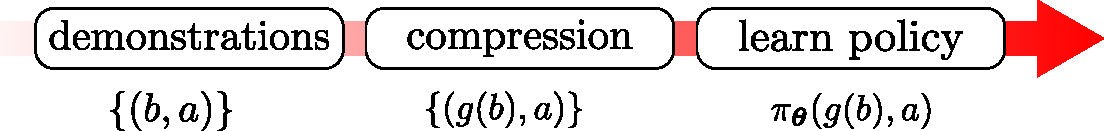
\includegraphics[width=0.8\textwidth]{./ch2-Background/Figures/belief_pipeline.pdf}
 \caption{Three steps in learning a POMDP policy from human demonstrations: First gather the belief-action dataset, second compress the beliefs and third 
 learn a generative policy.}
 \label{fig:belief-pipeline}
\end{figure}

This is the general 
concept but there are a few caveats which make this task not as straight forward as it seems.

\begin{itemize}
 \item \textbf{The belief state is unknown}: When the robot apprentice is watching the human perform a search task under state uncertainty, it is 
 unable to observe the belief state of the human. All that the agent can observe directly are the actions of the teacher. We make \textbf{two assumptions}, the first 
 is that the apprentice can infer the observations of the teacher by examining the teachers relation with the environment and secondly the initial uncertainty of the 
 teacher is assumed to be known. From these two assumptions, the sequence of belief states can be inferred via a Bayesian filter. This implies that  the mental 
 belief state of the human teacher is in fact known given the assumptions. We give more details in Chapter 3 on the validity of these assumptions
 and discuss their relation to Bayesian Theory of Mind (BoTM).
 
 \item \textbf{Learning a policy as a function of non-parametric beliefs:} Given that we are considering high levels of uncertainty and the 
 observations are sparse, in the form of contacts, no parametrisation of the belief in terms of a Gaussian function would be adequate. In this thesis all the considered beliefs will be from the non-parametric 
 Bayesian filter family, such as particle filters, which allows for a lot of flexibility. Learning a policy directly as a function of a particle filter is intractable. First 
 in non-parametric filters there is typically thousands of states and in efficient particle filters the number of parameters varies over time.
 We \textbf{compress the belief} into the most likely state and the entropy. In this way the size of the belief state is fixed and low dimensional.
\end{itemize}
 
\begin{figure}
 \centering
 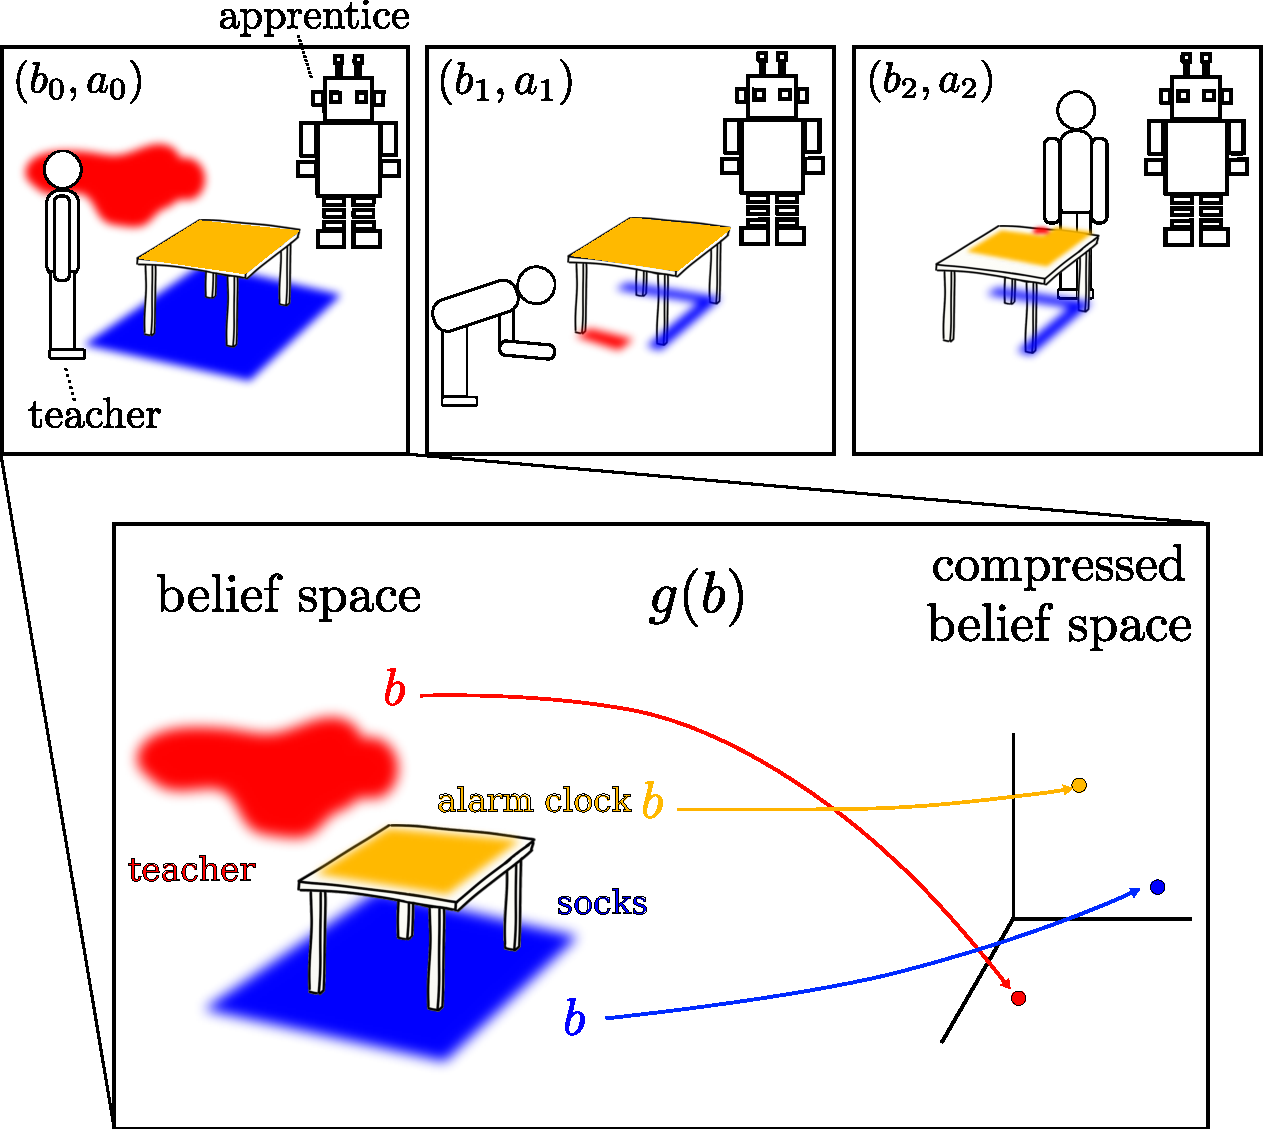
\includegraphics[width=\textwidth]{./ch2-Background/Figures/human_search.pdf}
 \caption{\textbf{Demonstrations:} An apprentice is looking at a human teacher who is searching for the
 alarm clock's button and his pair of socks. The apprentice assumes the structure of the original beliefs the human teacher has with respect to his 
 position and that of the alarm clock and socks, these are represented by the red, yellow and blue density functions. \textbf{Compression:} Given the data set of beliefs and actions obtained from the demonstrations, the beliefs 
 is compressed to a fixed parametrisation. \textbf{Learn policy:} A generative policy, $\policy(g(b),a)$ is learned from the actions and compressed beliefs and can be executed 
 according the schematic on the right. SE represents any Bayesian state space estimator, which takes as input, the current observation, belief and action and outputs the next 
 belief state.}
 \label{fig:human_search}
\end{figure}

In Figure \ref{fig:human_search} we illustrate an example of human teaching an apprentice robot how to search for 
objects (alarm clock and socks) in a state of high uncertainty, the human is blindfolded. Given what the apprentice can 
observe he must infer the beliefs of the teacher (red, blue and orange probability density functions).

\begin{itemize}

 \item \textbf{Reactive policy}: The control loop cycle, which computes the belief state, compresses it, and computes the 
 resulting action to take, should happen at around 10 to 100 Hz. This range may seem arbitrary but is in fact based on the humans control ability which at the highest
 cognitive level a delay in response is around 100ms and at the lowest reflex level at around 10-20 ms \cite{Biomechanics_2009}. This is to draw attention that the 
 full control loop, belief filtering, compression and action prediction should all happen within this range. See Figure \ref{fig:control_architecture} for 
 an illustration of the control architecture used.
 
 \item \textbf{Scalable belief filter}: In scenarios in which there are multiple objects being searched for by a human teacher, the joint belief distribution 
 of a non-parametric Bayesian state space filter will become quickly computationally intractable. This motivates the development of a new type of SLAM filter methods
 which can scale in situations in which observations are very sparse.
\end{itemize}

All of the above points are the motivation behind many of the decision choices we take and use in the subsequent chapters. 
They are necessary such to be able to successfully teach robotic systems to act as humans in partial observable states.

\begin{figure}
 \centering
 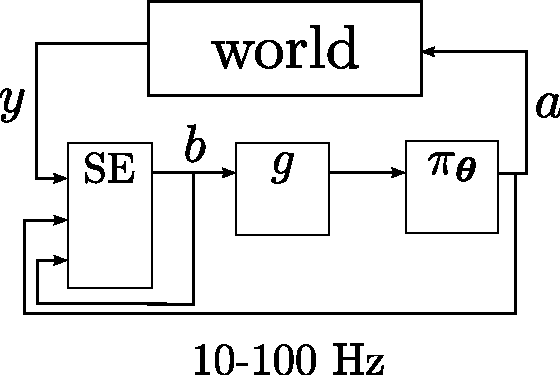
\includegraphics[width=0.4\textwidth]{./ch2-Background/Figures/control_loop.pdf}
 \caption{Control architecture of the apprentice robot. The control loop should run between 10-100Hz. Given an applied action, the world returns an observation 
 which is integrated by the State Estimator (SE) to give the current belief. The belief is the compressed and given as input to the policy.}
 \label{fig:control_architecture}
\end{figure}


 	\fi
\ifdefined	\gDisplaySearch			\chapter{Learning to reason with uncertainty as humans}
%
%	Need to make this stick with the previous Chapter !
%
%	-> 
%
The conclusions drawn from the literature survey in Chapter 2 are that non-heuristic methods for planning and control 
rely heavily on the initial data provided to their respective optimisers. An ideal initial set of behaviour should be comprised
of explorative and exploitative actions so that a final optimal policy can quickly achieve the balance between minimising 
uncertainty and solving the task at hand. This is especially true for Reinforcement Learning (RL) methods which make use of 
explorative actions to be able to find an optimal policy. In many RL applications random exploration or Gaussian noise perturbation
is sufficient to find an optimal policy. This is the case when either an exhaustive search of the action space is possible 
(mountain cart, inverted pendulum, etc...) or in policy search methods where the policy is parametrised by a few parameters.
In continuous action-state space POMDPs, when a generic non-parametric policy is desired  this is not feasible, especially 
when the decision horizon is long. Continuous action-state space POMDPs applications have predominantly focused on cases in which 
the uncertainty can be quantized by a single Gaussian parametrisation. This representation can be constraining since it requires 
the observation likelihood to be Gaussian as well. This assumption is restrictive and ill-suited for haptic search tasks in 
which observations are discontinuous and occur as impulses. 

In this chapter, we demonstrate that human foresight and intuition can be leveraged as a means of solving the 
exploration/exploitation dilemma under partial observable conditions. Human beings are versatile in their ability to 
accomplish tasks which are considered to be complex by current robotic standards. This perceived ability which we have over 
current robotic systems, due to our prior domain knoweldge and experience, can be extracted, encapsulated and transferred 
to a robot apprentice.

To demonstrate the application of the transfer of behaviour from a human teacher to a robotic apprentice we apply the framework outlined in Chapter 2, 
Section \ref{sec:approach} (PbD-POMDP) to a blindfolded haptic search task. In our blindfolded search task, both a robot and a human 
must search for an object on a table whilst deprived of vision and hearing, illustrated in Figure \ref{fig:searching}. 
The robot and human both have prior knowledge of the environmental setup making this a specific search problem with no required mapping of the environment, also known as active localisation. 
In Figure \ref{fig:searching}, a human has his sense of vision and hearing impeded, making the perception of the environment partially observable and 
leaving only the sense of touch available for solving the task. The hearing sense is also impeded since it can 
facilitate localisation when no visual information is available and the robot has no equivalent giving an unfair 
advantage to the human. By impeding hearing we align the perception correspondence between the human and robot.

By representing the belief of the human's position in the environment by a Particle Filter (PF) and learning a mapping from this belief 
to hand actions (velocities) with a Gaussian Mixture Model (GMM), we can model the human's search process and reproduce it for any agent. 
We further categorize the type of behaviours demonstrated by humans as being either risk-prone or risk-averse and find that more than 70\% of 
the human searches were considered to be risk-averse. We contrast the performance of this human-inspired search model with respect to Greedy and Coastal Navigation search methods. 
Our evaluation metric is the distance taken to reach the goal and how each method minimises the uncertainty.
We further analyse the control policy of the Coastal Navigation and GMM search models and argue that taking  uncertainty
into account is more efficient with respect to distance travelled to reach the goal.

\begin{figure}[h]
  \centering
  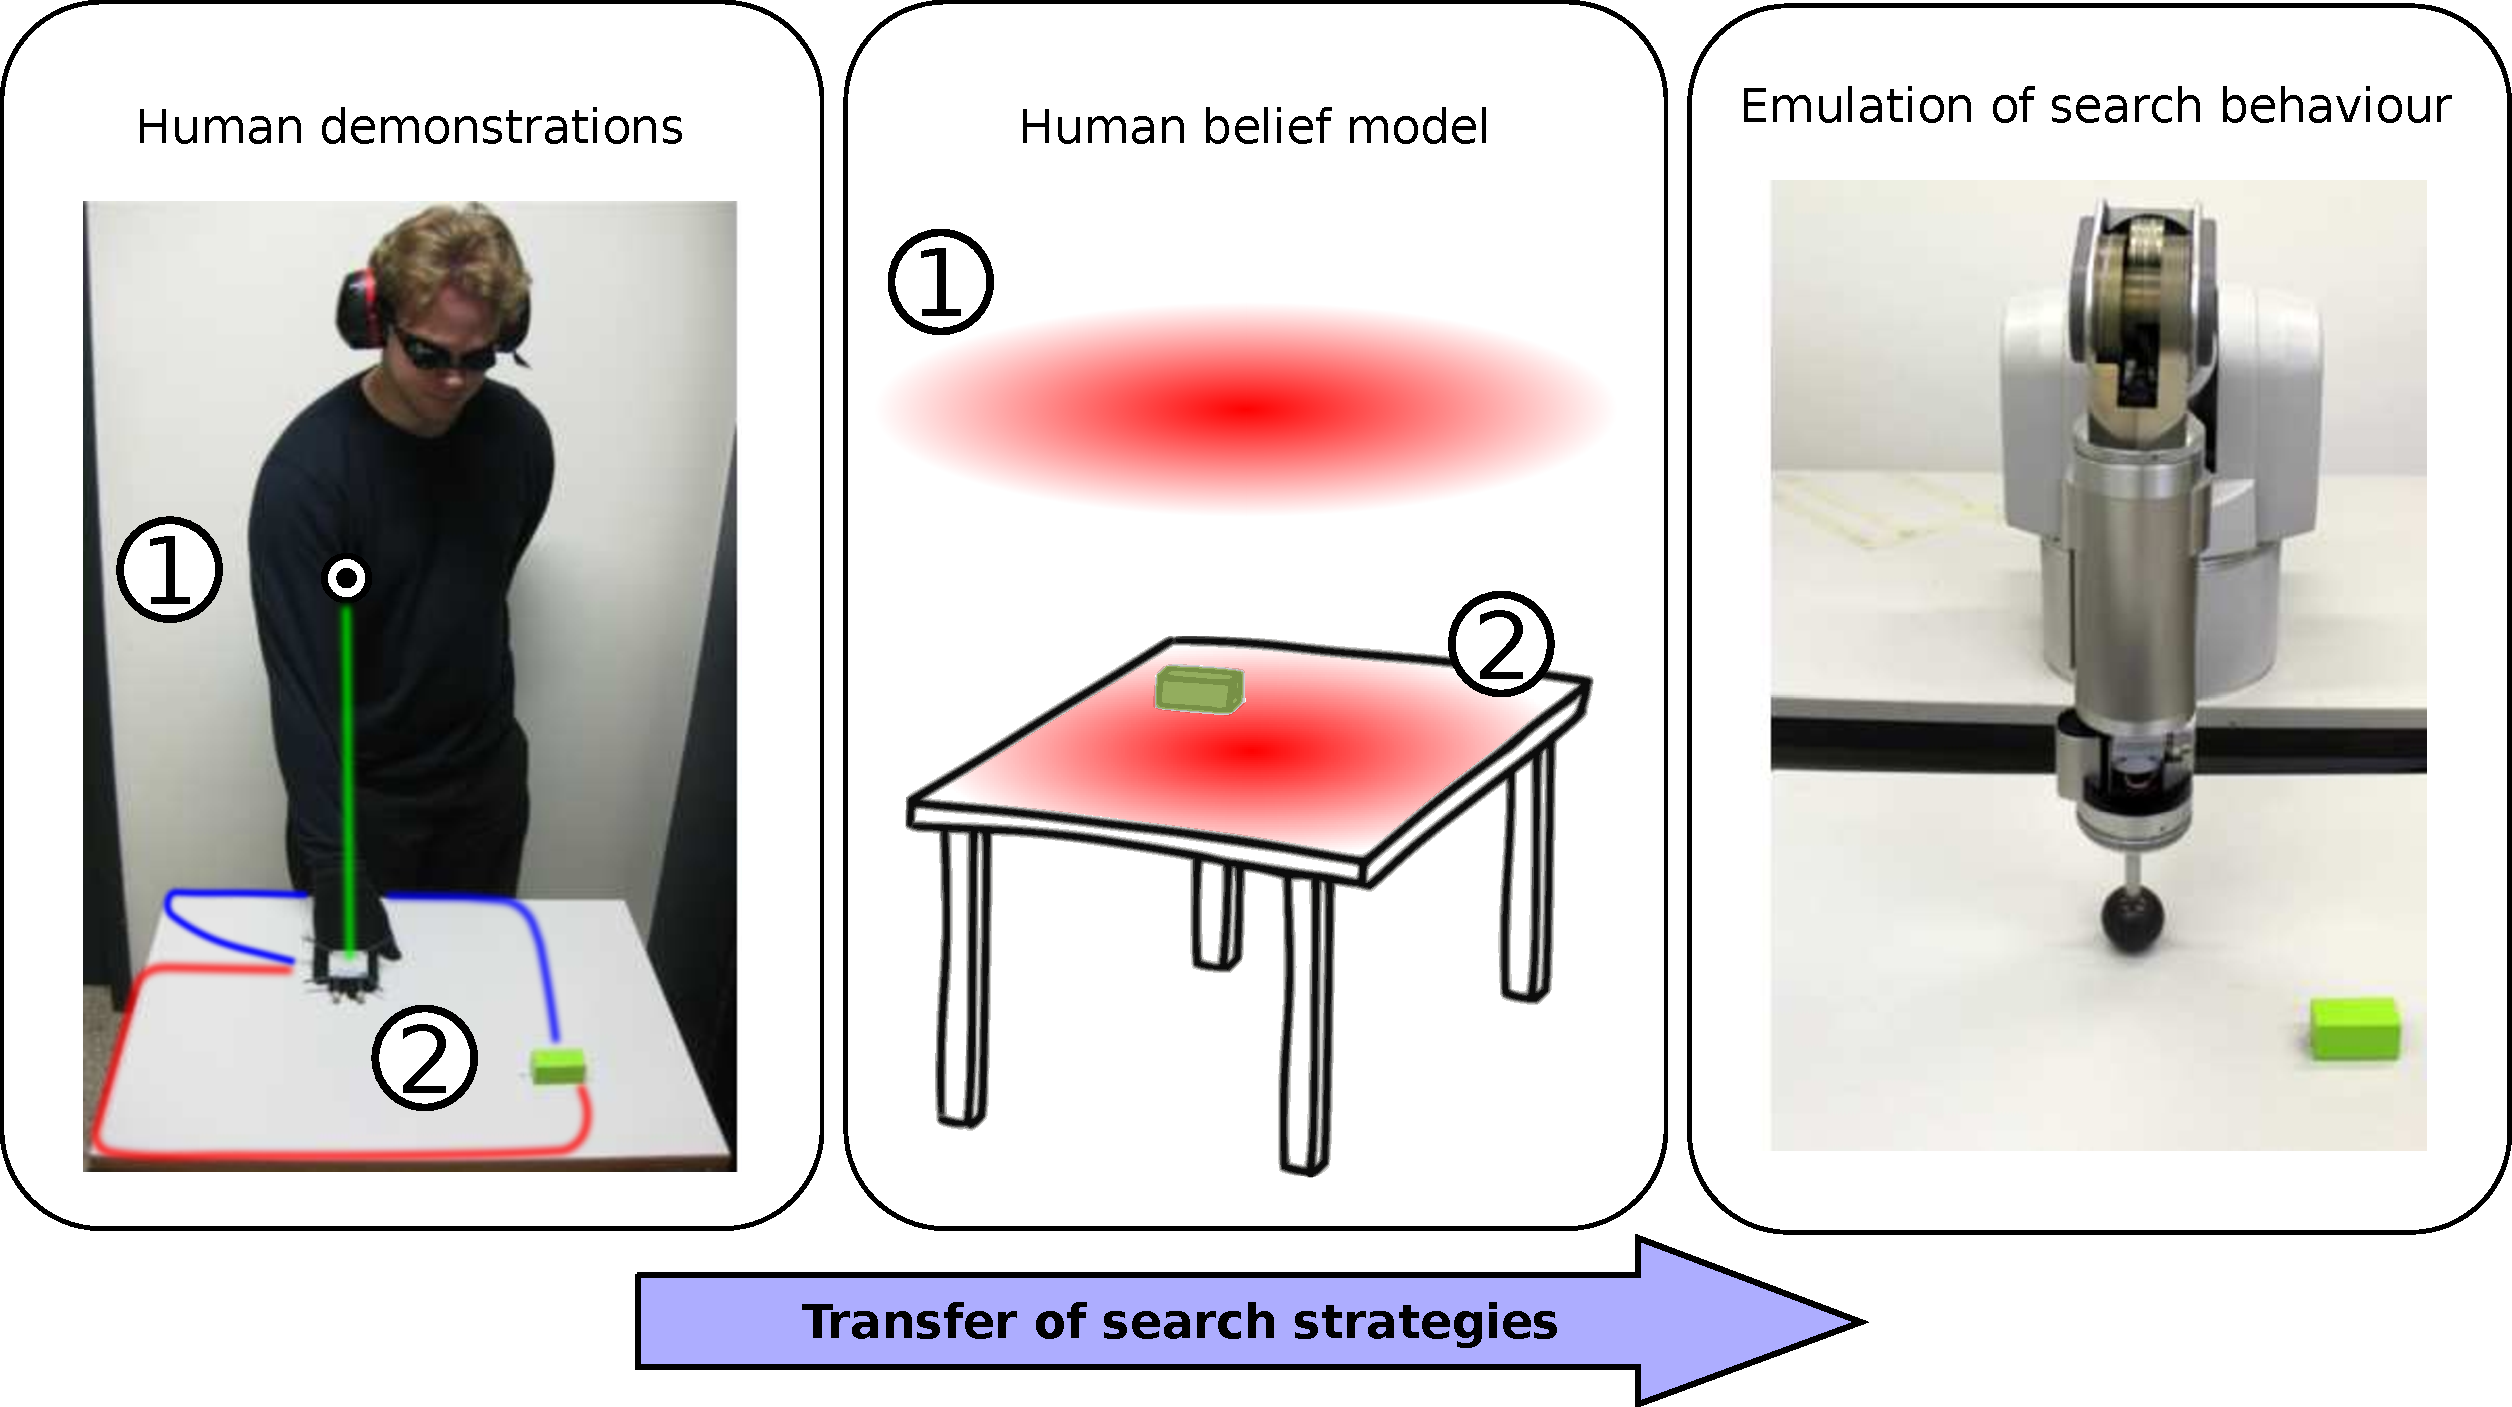
\includegraphics[width=0.95\textwidth]{./ch3-Search/Figures/Figure1.pdf}
  \caption{\textbf{Blindfolded search task} \textit{Left:}  Search task, a human demonstrator searching for the green wooden block on the table given
  that both his hearing and vision senses have been impeded. He starts (hand) at the white spot near position (1). The the red and blue trajectories 
  are examples of possible searches.
  \textit{Middle:} Inferred belief the human might have with respect to his position. If the human always starts at (1) and his belief is known, all 
  following beliefs (2) can be inferred from Bayes rule. \textit{Right:} WAM Robot 7 DOF
  reproduces the search strategies demonstrated by humans to find the object.}
 \label{fig:searching}
\end{figure} 

There are \textbf{two assumptions} we make when applying Programming by Demonstration, PbD (also known as Imitation Learning), to the POMDP task described above. 
The first assumption is that the human teacher's \textit{spatial cognitive} abilities are good enough to accomplish 
the task in a consistent fashion. In other words demonstrations should not be random and a pattern exists. The second assumption is that human's beliefs inferred  
by the apprentice are close to the actual belief of the human. 

\section{Outline}

\begin{itemize}

\item  \hyperref[ch3:background]{\ref{ch3:background}   Background}\\
We review aspects of the literature in robotics and cognitive science which are related to spatial navigation which 
consider scenarios with limited perceptual information. We review related literature from \textit{Spatial Navigation}, 
\textit{Theory of Mind} and \textit{Programming by Demonstration}.

\item  \hyperref[ch3:experiment]{\ref{ch3:experiment}   Experiment}\\
The table search experiment protocols are described and we detail how to learn and transfer search strategies from human teachers to a robot 
apprentice. A total of 15 human teachers participated and each gave 10 demonstrations, giving a total of 150 searches.

\item  \hyperref[ch3:formulation]{\ref{ch3:formulation}  Formulation}\\
We detail the implementation of the human belief in terms of a Particle Filter (PF). This includes the measurement and motion 
models. We describe how we compress the belief particle filter in terms of the most likely state and differential entropy.

\item  \hyperref[chap3:policies]{\ref{chap3:policies} 	Policies}
\begin{itemize}
  \item \hyperref[chap3:GMM_policy]{\ref{chap3:GMM_policy} Modelling human search strategies}\\
  We detail the implementation and parametrisation of a Gaussian Mixture Model (GMM) policy encapsulating
the human search strategies and how it synthesises new searches.
  \item \hyperref[chap3:costal_policy]{\ref{chap3:costal_policy} Coastal Navigation}\\
  We detail the implementation of a Coastal Navigation policy, used as a comparison with the GMM policy.
\end{itemize}

\item  \hyperref[chap3:results]{\ref{chap3:results} 	Results}\\
We conduct three types of analysis: we quantify the behaviour present in humans and policies in terms of riskiness; we 
qualitatively evaluate the differences between the GMM policy learned from human demonstrations and the Coastal Navigation policy;
we evaluate the distance taken to find the goal for a set of four search policies, including the GMM.

\end{itemize}

\section{Background}\label{ch3:background}

%\subsection{Acting under partial observability}
%Learning controllers or policies to act within a context where the state space is partially observable is of high relevance to all real 
%robotic applications. Resulting from limited and inaccurate perceptual information, often only an 
%approximation of the environment is available at any given time. If this inherent uncertainty is not taken 
%into account during planning or control there is a non-negligible risk of missing goals, getting lost and 
%wasting valuable resources. 



%A major difficulty faced in spatial cognitive navigation and within the context of our PbD-POMDP framework is that 
%the biological and neurological processes which are responsible for the observed behaviour during the experimental studies 
%are unobservable. Even with the increasing usage of neuro-imaging techniques such as functional Magnetic Reasons Imaging (fMRI)
%and electroencephalogram (EEG), whose technical aspects impose limitations on the possible experimental studies, it is hard to 
%determine a cognitive mathematical model of the underlying processes present in spatial navigation. 

\subsection{Spatial navigation}
%
%	Take away points: 1) Humans and animals are currently better than robots in doing this.
%		          2) Limitations of the quality of our policy depend on our working memory.
%

Spatial navigation, \cite{Wang_2007}, \cite{what_det_our_nav_ability_2010}, focuses on the role that sensory perception 
(vision, vestibular, proprioception ...), motor control and mental cognition have on the navigational ability of  
humans, animals and insects. A central aspect of spatial navigation is the way in which we mentally represent the geographical world, known 
as a \textit{cognitive map} (mental representation of environment first proposed by Tolman, 1948) and how we update our pose estimation 
in this map. The aspects of both  construction and correction of a cognitive map have been studied in great depth, \cite{spatial_updating_2008}.
There is reported evidence that we use both vestibular and proprioception in inferring self-motion in order to update our position through dead reckoning (also known as path integration). 
Given the estimated position we then use external cues such as geometric (the shape of a room) and features (the colour of the walls), 
to correct our position. The actual representation of our position and environment in our cognitive map has been proposed,
\cite{spatial_memory_how_ego_allo_combine_2006}, to be either encoded in our own frame of reference (egocentric) or in a frame of reference which 
is independent to us (allocentric) and acts like a standard paper map or both. This cognitive map enables us to reason about the relations between our own position and that of other items and landmarks present. 
This representation also facilitates our ability to localise ourselves and plan novel routes when needed.

In \cite{updating_egocentric_human_navigation_2000}, the authors studied the effect that disorientation has on blindfolded subjects' ability 
to recover their heading, which is necessary for re-localisation. Through eight different experiments they concluded that humans 
have an egocentric cognitive map.


Studies have also looked at the difference between congenitally blind, late blind and sighted people in their ability to encode ego-allocentric cognitive maps.
In \cite{Pasqualotto2013175}, the authors dispose a set of seven objects (brush, slipper, pan, dish, book, spoon, bottle) in the form of 
an array in a 12.5m $\times$ 9m room. The objects are positioned on top of stools. During a training phase, ten congenitally blind, ten late blind and ten blindfolded sighted people were taken through 
the setup and touched all objects present. This guided exploration (the experimenter leading the subject through the object array) was repeated until 
the participants could correctly recall all the objects' locations twice consecutively without help. In a testing room (no objects present) 
the participants were asked ``Judgement of Relative Direction''  questions and the accuracy and response time were recorded. From the results the authors 
concluded that blindfolded and late blinded participants used a allocentric representation of the object array, whilst the congenital blind 
subjects use an egocentric model. The cause of this difference is attributed to the role played by vision in the development of the 
multisensory brain area, in which vision is necessary for the development of an allocentric model. 

Many similar experiments have been conducted and a summary can be found in the following review \cite{spatial_memory_how_ego_allo_combine_2006},
where the authors explicitly state that a consensus has formed; both egocentric and allocentric representations of the environment are 
working in parallel. Current questions ponder whether allocentric models are part of the semantic memory as opposed to the procedural 
memory used by the egocentric model.

\subsubsection{Spatial cognition and memory}

The quality of the human teacher in  search tasks, which are partially observable in the terms of absence of vision,
will strongly depend on the teacher's ability to maintain an accurate cognitive map of his environment. This implies
that the size of the environment and search task will have an effect on the teacher's ability to provide near optimal 
demonstrations. 
Early and influential research into human's short term memory was presented in 1956 by George Miller in a seminal work, \cite{cogprints730} 
(22'780 citations), in which he described the ``so called'' magical number of our short term memory as being $7\pm2$ items, 
known as \textit{Miller's Law}. This research was conducted on a one dimensional task in which no spatial navigation was required.
Since then there have been many studies investigating the limits of short term memory.

In \cite{human_stsm_2015} a set of subjects had to find either 1, 3, 5 or 7 goal pads, among a grid array of 23 pads in a 4m $\times$ 4m room, 
within a 1 minute interval. They measured the subjects' error in terms of the number of locations visited before finding the goals. 
They found that on average the subjects had to visit ``$1.6 \times \#num\_goals$'' pads before achieving the task. The authors concluded 
that in this spatial navigation task there was no magical number which represents the limit of short term memory.
In another spatial navigation experiment, \cite{Iachini2014}, the effect that the scale of the environment 
has on the ego-allocentric representation is studied in blindfolded, late and early blind subjects. The main findings were
that cognitively blind people have more difficulty in developing an allocentric representation of the world. 
%In terms of difference in the scale of the problem (two conditions where compared, a task which required no locomotion and one that did), 
%only a small difference existed for the blindfolded subjects.

In \cite{stankiewicz2006lost}, a search task in a virtual maze is conducted by a set of human subjects.  The aim 
is to investigate the limitations that perception, memory and uncertainty have on human decisions in comparison 
with an ideal agent (POMDP solution). The authors' main findings were that as the size of the maze increases the
performance of the human subject decreases with respect to the ideal agent, as human subjects are limited by the 
uncertainty in their location and have difficulty in maintaining multiple hypotheses.

\subsubsection{Summary: spatial cognition}


The studies detailed above reported that if the environment is not overly large and complex our cognitive model is sufficient 
to produce policies which are on par with an optimal POMDP agent. 

Our study seeks to transfer exploratory behaviour from human teachers to a robot apprentice in a partially observable setting. 
In our search scenario the environment is less than 3 meters in length and 2 meters in depth with a single goal object to be found. 
Given this setup and the evidence from previous studies, humans should be able to achieve this task with a high level of proficiency. 

This is beneficiary since currently both humans and animals are better at spatial navigation than robots \cite{stankiewicz2006lost} 
especially when uncertainty is present. The quality of the demonstrations will strongly depend on the teacher's short term memory 
in retaining a sufficiently accurate cognitive map of the environment. 


\subsection{Human beliefs}

% Belief  
%In the Section \ref{sec:deci_un} on Decisions in Chapter 2, we introduced the concept of rationality for 
%both beliefs and desires. 

A crucial aspect for the success of PbD-POMDP learning is that the apprentice be able to infer 
the human's belief of his location whilst he is searching. In others words the apprentice
(human or robotic) has to infer the cognitive map of the teacher. 

%This is possible by observing the actions of teacher and guessing his perception 

The study of inference of another's mental state is part of Theory of Mind (ToM) \cite{Towards_a_ToM_2010}, which is concerned 
with our ability to infer beliefs, desires, intentions, perception,
goals and current knowledge. In this study, the apprentice will have to infer the teacher's beliefs which we assume are 
\textbf{rational}. A rational belief is a belief for which observations bring supportive evidence and 
gradually increase the certainty of the belief. In a recursive formulation this known as Bayesian Theory of Mind (BToM),
where the Bayesian component highlights the hypothesis that humans integrate information and update their beliefs in a similar 
fashion to Bayes rule.

Due to the complexity in the number of sensory sub-components, such as gaze following, and their interplay, required as a precursor to the development
of a ToM, much effort has been focused their  development.
Early work in implementing a ToM in a humanoid robot was introduced in \cite{ToM_humanoid} and is based on ToM models of \cite{Leslie_TOMM} 
and \cite{Baron-Cohen}. The author focused on building basic skills such as face finding and distinguishing animate and inanimate 
stimuli but left open the problem of the final interaction between all the components.

In \cite{MRF_ToM}, the authors model ToM as a Markov Random Field which defines a joint probability distribution over a set of
hidden actions and observation variables. The functions of these variables are hand-crafted for each experiment. 
The authors demonstrate that through a suitable parameterisation of the MRF they achieve results comparable to the predictions of ToM.
Recently in \cite{ToM_HRI_2106}, ToM and planning architecture have been integrated in a joint action collaborative human robot task, 
in which position, goal and action state of the human partner is maintained by his robotic assistant.

% ????
Work on modelling human beliefs and intentions has been undertaken in cognitive science, \cite{Bake_Saxe_Tene_2011}, 
\cite{Richardson1_Baker1_Tenenbaum1_Saxe1_2012}. In \cite{Bake_Tene_Saxe_2006}, the authors present a Bayesian framework 
for modelling the way humans reason and predict actions of an intentional agent. The comparison between 
a generic Bayesian model and the humans' predictions yielded similar inference capabilities.
This when asked to guess the intentions of a goal oriented agent in a 2D world, which both the Bayesian model and the 
humans were observing. This provided evidence supporting the hypothesis that humans integrate information using Bayes rule. 
Further, in \cite{Bake_Saxe_Tene_2011}, a similar experiment was performed in which the inference capabilities of humans,
with regard to both belief and desire of an agent, were comparable to that of their Bayesian model. Again they found
the human's inference was comparable to that of the Bayesian model.

In our PbD-POMDP framework we make a similar hypothesis that humans integrate information in a Bayesian way, however in a 
continuous domain. We infer the belief that humans have of their location in the world during search tasks.

\subsection{Programming by demonstration \& uncertainty}

%% Programming by Demonstration  Imitation Learning
Programming by demonstration (PbD) is advantageous in the POMDP and MDP contexts since it removes the need to perform the time 
consuming exploration of the state-action tree to discover an optimal policy and does not rely on any exploration 
heuristics to gather a sufficient set of belief points (as in point based value iteration methods discussed in Chapter 2).

We expect humans to perform an informed search. In contrast to stochastic sampling methods, 
humans utilise past experience to evaluate the costs of their actions in the future and to guide their search. This foresight and experience are implicitly encoded 
in the parameters of the model we learn from the demonstrated searches.

PbD has a long history in the autonomous navigation community. In \cite{Kasper2001153}, behaviour primitives of 
the PHOENIX robot control architecture are incrementally 
learned from demonstrations. Two types of behaviour namely \textit{reactive} and \textit{history-dependent} are 
learned and are encoded by radial basis functions. The
uncertainty is implicitly handled by directly learning the mapping between stimulus and response. In \cite{Hamner_2006_5810} the parameters of a
controller which performs obstacle avoidance are learned from human demonstrations. The uncertainty is inherently handled 
by learning the relation between sensor input and control output. In \cite{LfD_Autonomous_Navigation_in_Complex_Unstructured_Terrain} the objective function of a path planner is learned from human demonstrations. 
The objective function is a weighted sum of features corresponding to raw sensor measurements. This is another example where the partial information of the state is 
taken into account at the perception-action level, with the difference that instead of a policy being learned the objective function from which it is generated is learned. 

% Uncertainty is in the dynamics
Uncertainty is not restricted to state estimations but can also present in dynamical interaction with the environment in which 
unforeseen and perceptual uncertainties can arise such as in manipulation tasks. When solely tracking a Cartesian trajectory 
position uncertainties (poor visual estimation of the target) can lead to the failure of the task or a dangerous accumulation 
of contact forces. In \cite{online_pre_sensor_2011} the authors learn, via imitation learning, an initial 
Dynamic Movement Primitive (DMP) Cartesian policy and separately a target a force profile. By using sensor feedback they 
modify the target trajectory such to replicate the force profile thus achieving robustness to pose uncertainty. Another possibility
is to vary the stiffness parameters of an impedance controller \cite{Klas_icra_2012} based on the position uncertainty, 
if the position uncertainty is high then the robot will be more compliant. In \cite{MedinaSH13} the authors introduce a 
risk-sensitive control framework which depending on the uncertainty will make a trade-off between the position and force errors parameter gains
of an impedance controller. The task (Cartesian position and velocity) which is tracked by the controller is learned from demonstrations and encoded in 
a model.

%In \cite{Nicolescu01learningand}, the authors learn how to combine low level pre-acquired action 
%primitives to achieve more complex tasks from human demonstrations, but 
%they do not consider the effect of uncertainty.



Much work has been undertaken in learning reactive-behaviour, history dependent behaviour and combining multiple behaviour primitives to achieve
complex behaviour. However very few have studied the effect of uncertainty in the decision process and 
do not consider it during the learning or assume that it is implicitly handled.
A noticeable exception is \cite{GeorgiosLidoris}, in which a human expert guides the exploration of a robot in an indoor environment. 
The high level actions (\textit{Explore}, \textit{Loop Closure}, \textit{Reach goal}) taken by the human are recorded along with three different features related to the uncertainty in the map. 
Using SVM classification a model is learned which indicates which type of action to take given a particular set of 
features. The difference with our approach is that we perform 
the learning in continuous action space at trajectory level and multiple actions are possible given the same state, which cannot be handled by a classifier.

%%%%%%%%%%%%%%%%%%%%%%%%%%%%%%%%%%%%%%%%%%%%%%%%%%%%%%%%%%%%%%%%%%%%%%%%%%%%%%%%%%%%%%%%%%%%%%%%%%%%%%%%%%%%%%%%%%%%%%%%%%%%%%%%%%%%%%%%%
%																	   %
%					Research Design and Methodology									   %
%																	   %
%%%%%%%%%%%%%%%%%%%%%%%%%%%%%%%%%%%%%%%%%%%%%%%%%%%%%%%%%%%%%%%%%%%%%%%%%%%%%%%%%%%%%%%%%%%%%%%%%%%%%%%%%%%%%%%%%%%%%%%%%%%%%%%%%%%%%%%%%

\section{Experiment: table search}\label{ch3:experiment}

In our search task setup, Figure \ref{fig:tab_search_task} and  Figure \ref{fig:experiment} (\textit{top left}), 
a group of 15 human volunteers were asked to search for a wooden green block located at a fixed position on a bare table. 
Each participant repeated the experiment 10 times from each of 4 mean starting points with an associated small variance. 
The starting positions were given with respect to the location of the human's hand (all participants where right handed). The humans were always facing the table with their right 
arm stretched out in front of them. The  position of their hand was then either in front, to the left, to the right, or in contact with the table itself. 

\begin{figure}
 \centering
   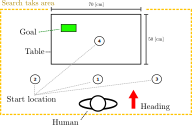
\includegraphics[width=0.8\textwidth]{./ch3-Search/Figures/experimentsetup}
  \caption{Table search task. Blindfolded human subjects after a disorientation step are placed in one of the 
  four starting locations. The heading of the subject is always kept the same. The human's objective is to locate
  the green block on the table. Throughout all experiments the green wooden block is kept in the same location.}
  \label{fig:tab_search_task}
\end{figure}
\begin{figure}
\centering
  \includegraphics[width=\textwidth]{./ch3-Search/Figures/Figure2}
  \caption{\textit{Top left}: A participant is trying to locate the green wooden block on the table
given that both vision and hearing senses have been inhibited. The location of his hand is being tracked by the
OptiTrack\textsuperscript{\textregistered} system. \textit{Top right:} Initial distribution of the uncertainty or belief we assume
the human has with respect to his position. \textit{Bottom left:} Set of recorded searches, the trajectories are with respect to the hand.
\textit{Bottom right:} Trajectories starting from same area but have different search patterns, the red trajectories all navigate to the goal
via the top right corner as opposed to the blue which go by the bottom left and right corner. Among these two groups there are trajectories which
seem to minimize the distance taken to reach the goal as opposed to some which seek to stay close to the edge and corners.}
\label{fig:experiment}
\end{figure}


As covered in the background section, previous work has taken a probabilistic Bayesian approach to model the beliefs and intent 
of humans. A key finding was that humans update their beliefs using Bayes rule (shown so far in the discrete case). 
We make a similar assumption and represent the human's location belief (where he thinks he is) by a particle filter which
is a point mass representation of a probability density function. There is no way of
knowing the human's belief with certainty. We make the critical assumption that the belief is observable in the first time step of the search and all following beliefs 
are assumed correct through applying Bayes integration.
The belief is always initialized to be uniformly distributed on top of the table, 
see Figure \ref{fig:experiment} (\textit{top right}), and the starting position of the human's hand is always in this area.

Before each trial the participant was told that he/she would always be facing the same direction with respect to the table (so always facing the goal, 
like in the case of a door) but his/her translational starting position would vary. 
For instance, the table might not be always directly in front of the person and his/her distance to the edge or 
corner could be varied. In Figure \ref{fig:experiment}
\textit{bottom left}, we illustrate four representative recorded searches whilst in the \textit{bottom right}, we illustrate a set of trajectories 
which all started from the same region. One interesting aspect is the diversity present,
demonstrating clearly that humans behave differently given the same situation.  

It is non-trivial to have a robot learn the behaviour exhibited by humans performing this task. As we cannot encapsulate the true complexity of 
human thinking, we model the human's state through two variables, namely, the human's uncertainty about his current location and the human's  
belief of his position. The various strategies adopted by humans are modelled by building a mapping from the state variables to actions, which are the motion of 
the human arm. Aside from the problem of correctly approximating the belief and its evolution over time, the model needs to take into consideration
that people behave very differently given the same situation. As a result it is not just a single strategy that will be transferred but rather a mixture 
of strategies. 


\section{Formulation} \label{ch3:formulation}

In the standard PbD formulation of this problem, a parametrised function is learned,
mapping from state $x_t$, which denotes the current position of the demonstrator's hand, to  
the hand's displacement $\dot{x}_t$. In our case since the environment is partially observable 
we have a belief or probability density function, $p(x_{t}|y_{0:t},\dot{x}_{0:t})$, which is conditioned on all 
sensing information, $y_{0:t}$, (the subscript, $0:t$, indicates the time slice which ranges from, $t=0$, to 
the current time, $t=t$) over the state space at any given point in time and the history of applied actions, $a_{0:t}$. 
We seek to learn this mapping, $f : p(x_{t}|y_{0:t},\dot{x}_{0:t}) \mapsto \dot{x}_{t+1}$, from demonstrations. During 
each demonstration we record a set of variables consisting of the following:

\begin{itemize}
 \item $\dot{x}_t \in \mathbb{R}^{3}$, velocity of the hand in Cartesian
space, which is normalised. 
 \item $\hat{x}_t = \operatorname*{arg\,max}_{x_t} p(x_{t}|y_{0:t},\dot{x}_{0:t})$, the most likely position of the
end-effector, or believed position.
 \item $U \in \mathbb{R}$, the level of uncertainty which is the entropy of the belief: $H\left(p(x_{t}|y_{0:t},\dot{x}_{0:t})\right)$.
\end{itemize}
A statistical controller was learned from the tuple dataset: $\{(\dot{x},\hat{x},U)\}$ recorded during the search 
trials of the human subjects. Having described the experiment we proceed to give an in-depth description 
of the mathematical representation of the belief, sensing and motion models and the uncertainty. 


\subsubsection{Belief model}


A human's belief of his location in an environment can be multi-modal or uni-modal, Gaussian or non-Gaussian and may change from one distribution to another. 
We chose a particle filter to be able to represent such a wide range of probability distributions. A particle filter is a Bayesian probabilistic method 
which recursively integrates dynamics and sensing to estimate a posterior from a prior probability density. The particle filter has two elements. The first 
estimates a distribution over the possible next state given dynamics and the second corrects it through integrating sensing. Given 
a \textit{motion model} $p(x_{t}|x_{t-1},\dot{x}_{t})$, and a \textit{sensing model} $p(y_{t}|x_{t})$, we recursively apply a 
prediction phase where we incorporate motion to update the state, and an update phase where the sensing data is used to 
compute the state's posterior distribution. The two steps are depicted below.

\begin{eqnarray}
 p(x_{t}|y_{0:t-1},\dot{x}_{0:t}) &=& \int p(x_{t}|x_{t-1},\dot{x}_{t})\,p(x_{t-1}|y_{0:t-1},\dot{x}_{0:t-1})\,dx_{t-1} \\
 p(x_{t}|y_{0:t},\dot{x}_{0:t}) &=& \frac{p(y_{t}|x_{t})p(x_{t}|y_{0:t-1},\dot{x}_{0:t})}{p(y_{t}|y_{0:t-1})}
\end{eqnarray}

The probability distribution over the state $p(x_{t}|y_{0:t},\dot{x}_{0:t})$ is represented by a set of weighted particles which represent hypothetical
locations of the end-effector and  their density which is proportional to the likelihood. The particular particle filter used was the 
\textit{Regularised Sequential Importance Sampling} \cite[p.182]{Arul_Mask_Clap_2002}. From previous literature \cite{Bake_Saxe_Tene_2011} 
it has been shown that there is a similarity between Bayes update rule and the way humans integrate information over time. Under this assumption 
we hypothesise that if the initial belief of the human is known then the successive update steps of the particle filter should correspond to a good approximation 
of the next beliefs. 

\subsubsection{Sensing model}

The sensing model tells us the likelihood, $p(y_t|x_t)$, of a particular sensation $y_t$ given
a position $x_t \in \mathbb{R}^{3}$. In a human's case, the sensation of a curvature indicates the 
likelihood of being near an edge or a corner. However the likelihood cannot be modelled using 
the human's sensing information. Direct access to pressure, temperature and such salient information is not available. 
Real sensory information needs to be matched against virtual sensation at each hypothetical location $x_t$ of a particle. 
Additionally,  for the transfer of behaviour from human to robot to be successful, the robot should be
able to perceive the same information as the human, given the same situation. An approximation of what a human or robot senses 
can be inferred, based on the end-effector's distance to particular features in the environment. In our case four main features 
are present, namely corners, edges, surfaces and an additional dummy feature defining no contact, air. The choice of these features is prior knowledge 
given to our system and not extracted through statistical analysis of recorded trajectories. The sensing vector is $y_t = \left[p_c,p_e,p_s,p_a\right]$, 
where $p$ refers to probability and the subscript corresponds to the first letter of the feature it is associated with. In Equation \ref{eq:sensingfunction}, 
the sensing function, $h(x_t,x_c)$, returns the probability of sensing a corner, where $x_c \in \mathbb{R}^3$ is the Cartesian position of the corner which is
the closest to $x_t$. 

\begin{equation}\label{eq:sensingfunction}
  p_c = h(x_t,x_c;\beta) = \exp\left( -\left(\beta \cdot \|x_t - x_c\|\right)^2 \right)
\end{equation}

The exponential form of the function, $h$, allows the range of the sensor to be reduced. We set $\beta > 0$ such that 
any feature which is more than 1cm way from the end effector or hand has a probability close to zero of being sensed. 
The same sensing function is repeated for all feature types.

The sensing model takes into account the inherent uncertainty of the sensing function \ref{eq:sensingfunction}, 
and gives the likelihood, $p(y_t|x_t)$ of a position. Since the range of sensing is extremely small and entries are probabilistic 
we assume no noise in the sensor measurement.
The likelihood of a hypothetical location, $x_t$,  is related to Jensen-Shannon divergence (JSD), $p(y_t|x_t) = 1 - JSD(y_t||\hat{y}_t)$ , between true sensing vector,
$z_t$, obtained by the agent and that of the hypothetical sensation $\hat{y}_t$ generated at the location of a particle. In Figure \ref{fig:pf_example}, four 
different beliefs are shown.

\begin{figure}
  \centering
  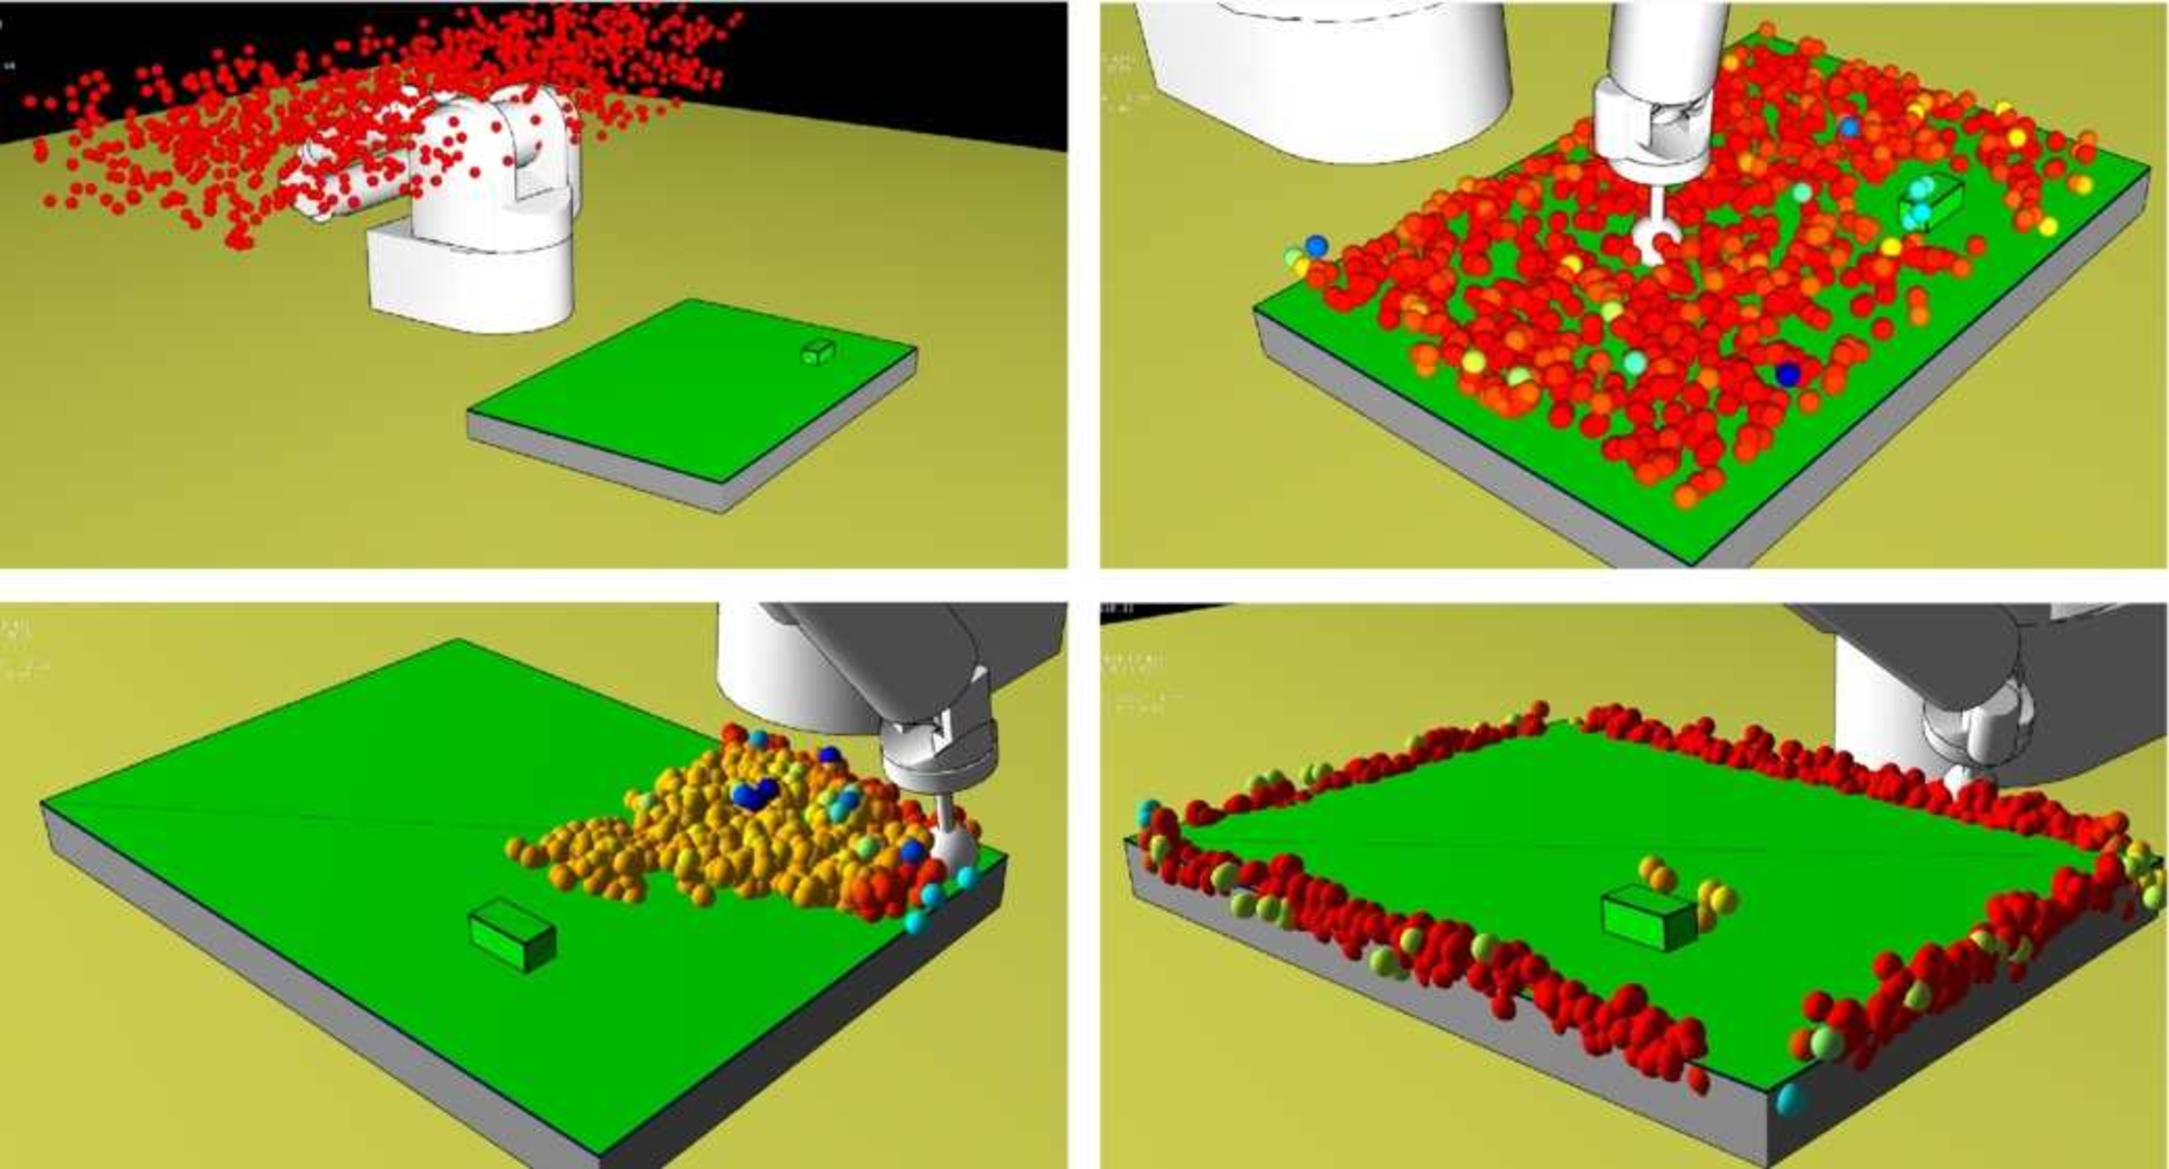
\includegraphics[width=\textwidth]{./ch3-Search/Figures/particlefilter.pdf}
  \caption{Four different time frames of the evolution of the belief particle filter. \textit{Top left}: Initial belief distribution; a lot of uncertainty.
  \textit{Top right:} First contact is made with the table, the measurement likelihood restrains the samples to be on the table's surface. \textit{Bottom right:}
  First contact is an edge. \textit{Bottom left:} Gradual localisation.}
  \label{fig:pf_example}
\end{figure}

\subsubsection{Motion model}

The motion model is straight forward compared with the sensing model. In the robot's case the Jacobian gives the next 
Cartesian position given the current joint angles and angular velocity of the robot's joints.
From this the motion model is given by $ p(x_{t}|x_{t-1},\dot{x}_{t}) = \mathrm{J}(q)\dot{q} + \epsilon$ where $q$ is 
the angular position of the robot's joints, $J(q)$ is the Jacobian and $\epsilon \sim \mathcal{N}(0,\sigma^{2}I)$ is white noise. 
The robot's motion is very precise and its noise variance is very low. For humans, the motion model is the velocity of the hand 
movement provided by the tracking system. In our experiment we consider the noise from motion to be negligible. An increase in 
uncertainty already results from the re-sampling stage of Sampling Importance Resampling (SIR) particle filter and we found 
no need to add additional motion noise.
The particles' positions were updated by applying the measured velocity obtained from either the visual tracking system 
(when recording the human demonstrations) or the robot's forward kinematics.

\subsubsection{Uncertainty}

% First motivate entropy as a natural method for computing the uncertainty

In a probability distribution framework, entropy is used to represent uncertainty. It is the expectation of a 
random variable's total amount of unpredictability. The higher the entropy the more the uncertainty, likewise the 
lower the entropy, the less the uncertainty. In our context, a set of weighted samples $\{w_{i},x_{i}\}^{i=1\dots N}$ replaces 
the true probability density function of the belief, $p_{\Param}(x_t|y_{0:t},\dot{x}_{0:t})$. A reconstruction of 
the underlying probability density is achieved by fitting a Gaussian  Mixture Model (GMM), Equation \ref{eq:gmm1}, to the particles,

\begin{equation}\label{eq:gmm1}
  p_{\Param}(x_t|y_{0:t},\dot{x}_{0:t}) = \sum\limits_{k=1}^{K} \piK\, g(x_t\: ;\MuK,\SigK )
\end{equation}
where parameters $\Param = \{w^{[k]},\MuK,\SigK\}_{1,\dots,K}$, are the weights, means and covariances of the individual multivariate Gaussian function, $g(\cdot)$ and
$K$ is the number of Gaussian components. The scalar $\piK$ represents the weight associated to mixture component $k$ 
(indicating the component's overall contribution to the distribution) and $\sum_{k=1}^{K} \piK = 1$. The parameters $\MuK \in \mathbb{R}^{(3\times 1)}$ 
and $\SigK \in \mathbb{R}^{(3\times 3)}$ are the mean and covariance of the normal distribution $k$. 

The main difficulty here is determining the number of parameters of the density function in a computationally efficient manner.
We approach this problem by finding all the modes in the particle set via mean-shift hill climbing and set these as the 
means of the Gaussian functions. Their covariances are determined by maximizing the likelihood of the density function 
via Expectation-Maximization (EM). 
%
%	images/clustering.eps
%

\begin{figure}
 \centering
   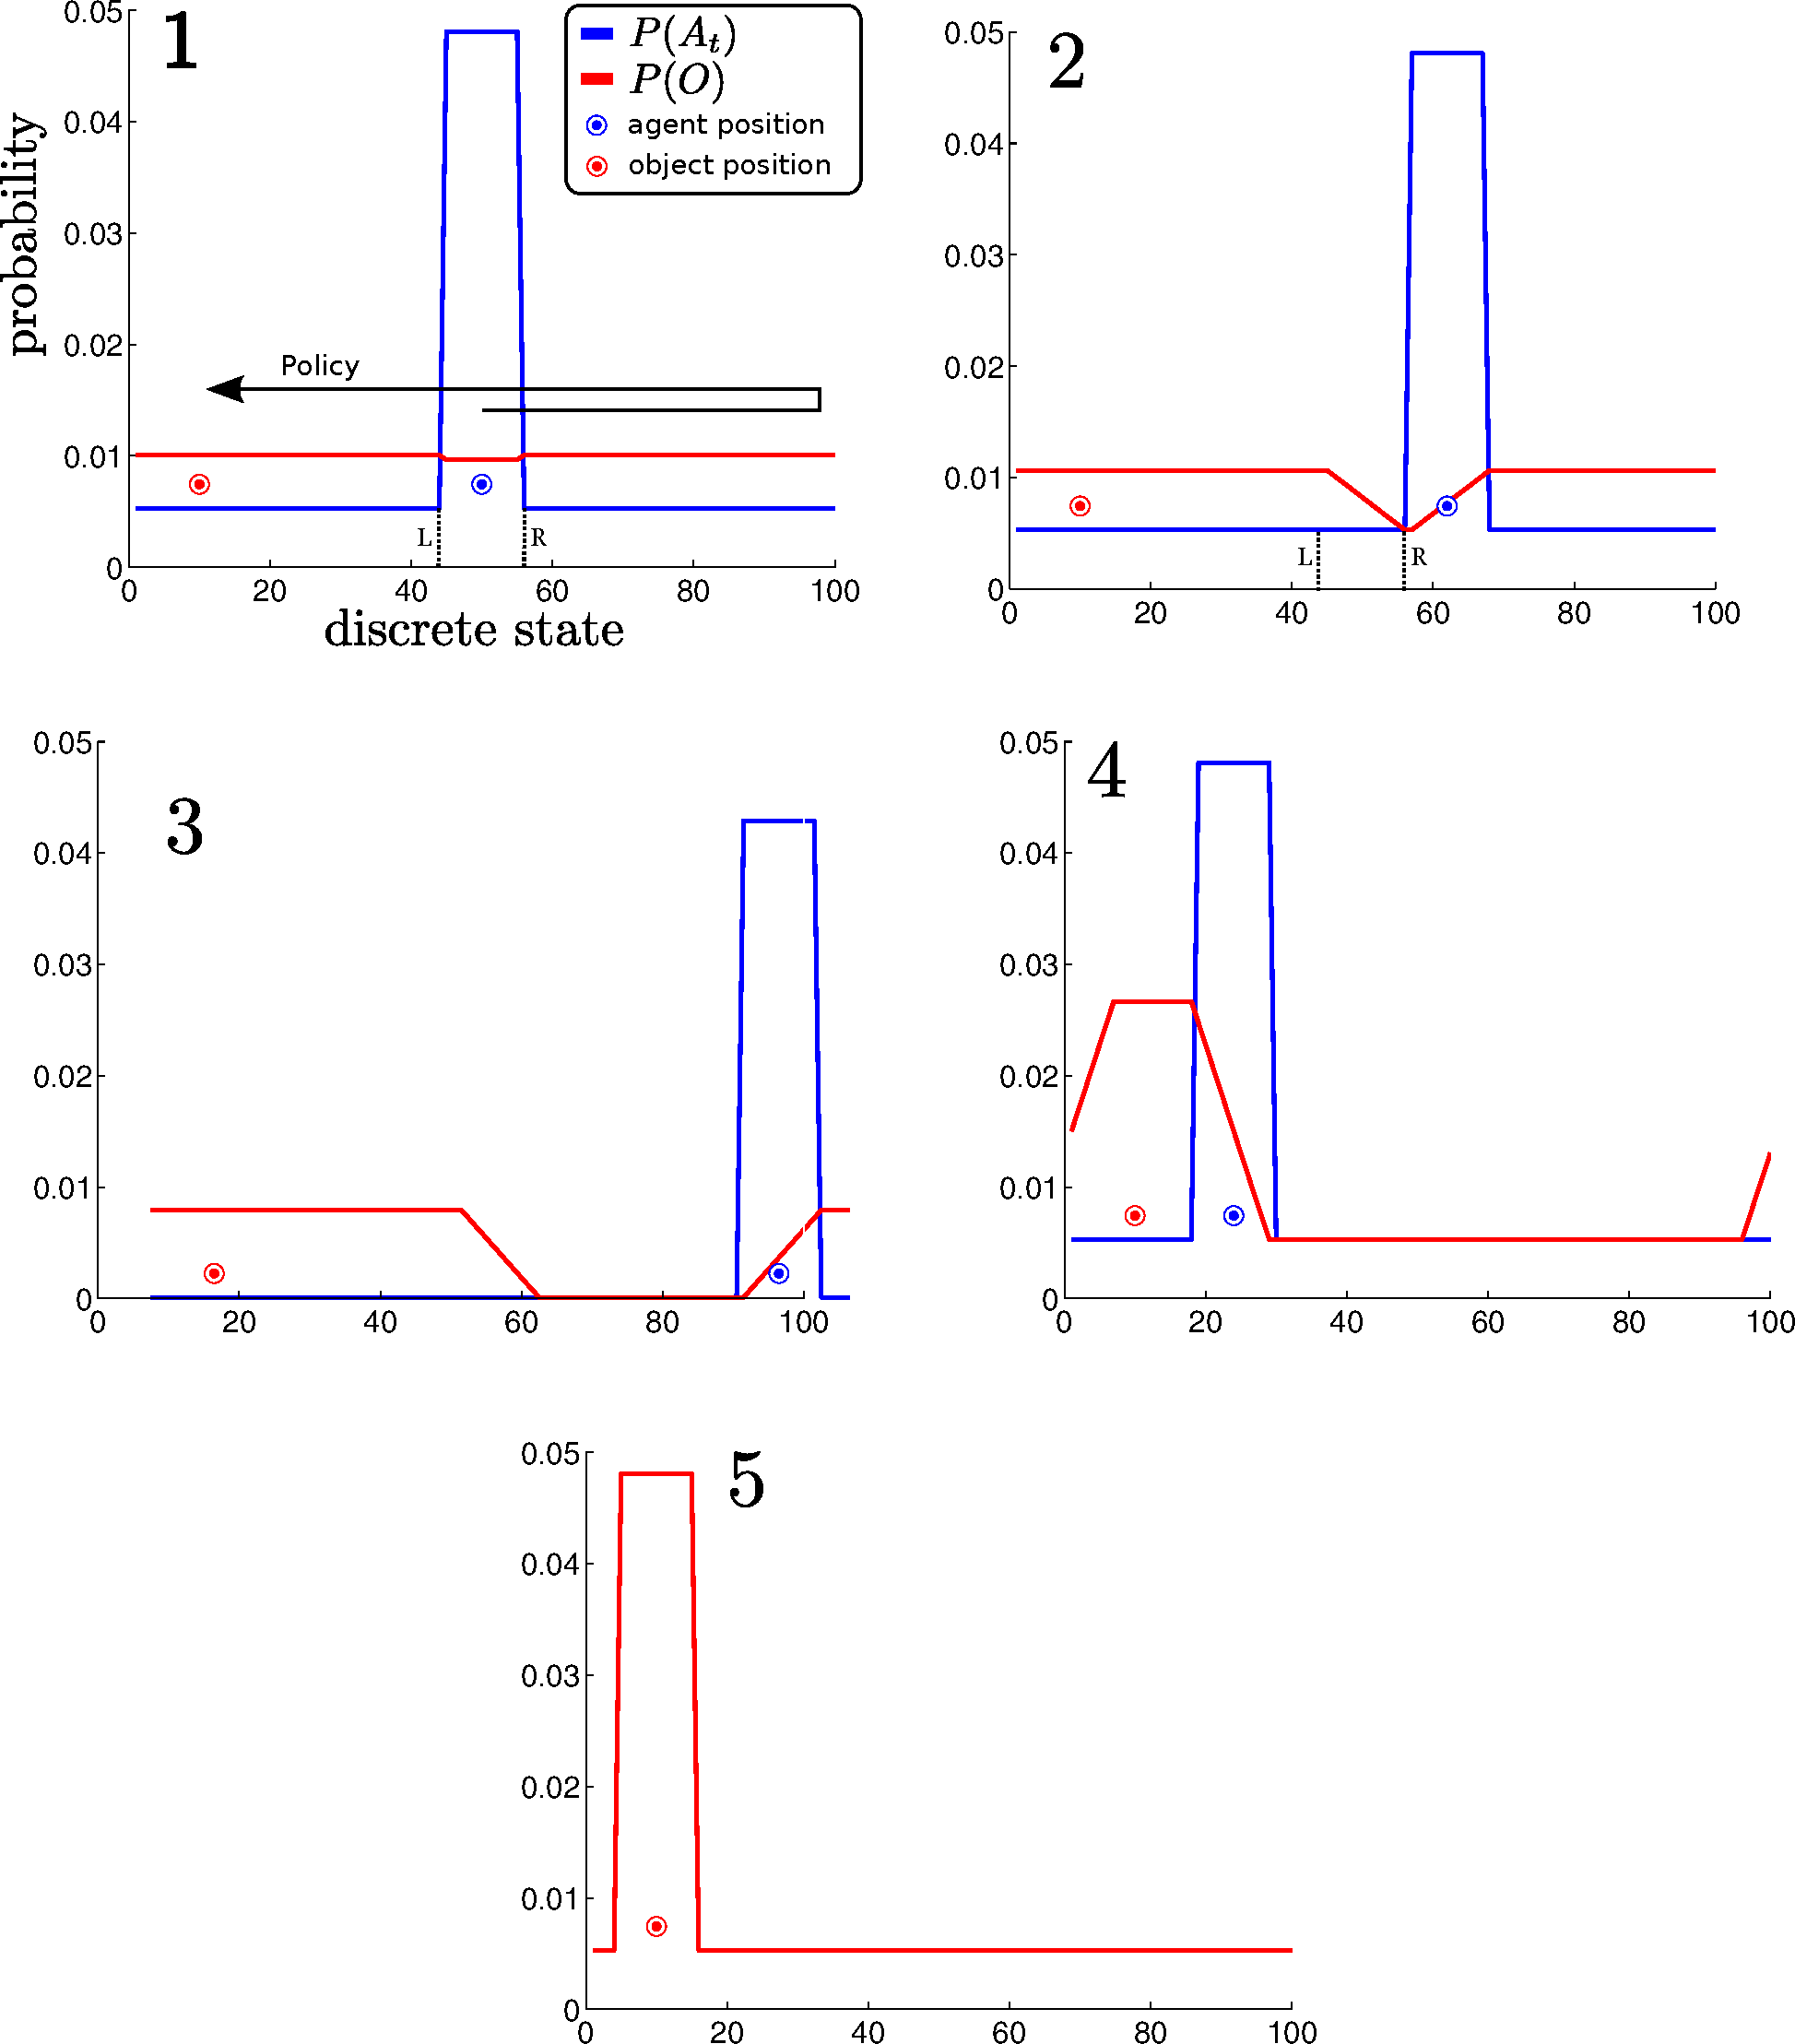
\includegraphics[width=0.95\textwidth]{./ch3-Search/Figures/Figure3}
  \caption{Representation of the estimated density function. \textit{Top Left and Right:} Initial starting point, 
  all Gaussian functions are uniformly distributed with uniform priors. The red cluster always has the highest likelihood which is taken
  to be the believed location of the robot's/human's end-effector. \textit{Bottom Left:} Contact with the table has been established, the robot location differers
  from his belief. \textit{Bottom Right:} Contact has been made with a corner, the clusters reflect that the robot could be at any corner (note that weights are not 
  depicted, only cluster assignment).}
  \label{fig:clustering}
\end{figure}

Given the estimated density we can compute the upper bound of the differential entropy \cite{DiffEntropyHuber2008}, $H$,
%which is taken to be the uncertainty $U$,
\begin{equation}
  H\left(  p_{\Param}(x_t|y_{0:t},\dot{x}_{0:t}) \right) = \sum\limits_{k=1}^{K} \piK\ \left( -\log(\piK) + \frac{1}{2} \log((2\pi e)^{D} |\Sigma_{k}|) \right)
\end{equation}
where $e$ is the base of the natural logarithm and $D$ the dimension (being 3 in our case).

The reason for using the upper bound is that the exact differential entropy of a mixture of Gaussian functions has no 
analytical solution. When computing both the
upper and lower bounds it was found that the difference between the two was insignificant, making any bound a good approximation 
of the true entropy. The choice of the believed location of the robot/human end-effector is taken to be the mean of the 
Gaussian function with the highest weighted $\pi$.

\begin{equation}
 \hat{x}_t = \operatorname*{arg\,max}_{x_t} p_{\Param}(x_{t}|z_{0:t}) = \mu_{(k = \max(w))}
\end{equation}

Figure \ref{fig:clustering} depicts different configurations of the modes (clusters) and believed position of the end-effector (indicated by a yellow arrow).  



%%%%%%%%%%%%%%%%%%%%%%%%%%%%%%%%%%%%%%%%%%%%%%%%%%%%%%%%%%%%%%%%%%%%%%%%%%%%%%%%%%%%%%%%%%%%%%%%%%%%%%%%%%%%%%%%%%%%%%%%%%%%%%%%%%%%%%%%%
%																	   %
%					Methods												   %
%																	   %
%%%%%%%%%%%%%%%%%%%%%%%%%%%%%%%%%%%%%%%%%%%%%%%%%%%%%%%%%%%%%%%%%%%%%%%%%%%%%%%%%%%%%%%%%%%%%%%%%%%%%%%%%%%%%%%%%%%%%%%%%%%%%%%%%%%%%%%%%


\section{Policies}\label{chap3:policies}

\subsection{Modelling human search strategies}\label{chap3:GMM_policy}

During the experiments, the recorded trajectories show that different actions are present for the same belief and uncertainty making the data multi-modal
(for a particular position and uncertainty different velocities are present). That is multiple actions are possible given a specific belief. 
This results in a one-to-many mapping which is not a valid function, eliminating any regression technique which directly learns a non-linear function. 
To accommodate this fact we use a GMM to model the human's demonstrated searches, $\{(x,\dot{x},U)\}$. 
Using statistical models to encode control policies in robotics is quite common, see \cite{Billard08chapter}. 

% explain how much data we have vs the number of gaussian components
By normalising the velocity the amount of information to be learned was reduced. We also took into consideration that velocity is more 
specific to embodiment capabilities: the robot might not be able to reproduce safely some of the velocity profiles demonstrated. 

The training data set comprised a total of 20'000 tuples $(\dot{x},\hat{x},U)$, from the 150 trajectories gathered from the demonstrators. 
The fitted GMM $\pi_{\Param}(\dot{x},\hat{x},U)$ had a total of 7 dimensions, 3 for direction, 3 for position and 1 scalar for uncertainty. 
The definition of the GMM is presented below in equation \ref{eq:gmm2}.

\begin{equation} \label{eq:gmm2}
 \pi_{\Param}(\dot{x},\hat{x},U) = \sum\limits_{k=1}^{K} \piK\, g(\dot{x},\hat{x},U\: ;\MuK,\SigK )
\end{equation}

\begin{equation*}
    \MuK =
    \begin{bmatrix}
      \mu_{\dot{x}} \\
      \mu_{\hat{x}} \\
      \mu_{U}
    \end{bmatrix}
    \SigK =
    \begin{bmatrix}
      \Sigma_{\dot{x}\dot{x}} & \Sigma_{\dot{x}\hat{x}} & \Sigma_{\dot{x}U} \\
      \Sigma_{\hat{x}\dot{x}} & \Sigma_{\hat{x}\hat{x}} & \Sigma_{\hat{x}U} \\
      \Sigma_{U\dot{x}} & \Sigma_{U\hat{x}} & \Sigma_{UU}   
    \end{bmatrix}
\end{equation*}
Given this generative representation of the humans' demonstrated searches we proceeded to 
select the necessary parameters to correctly represent the data. This step
is know as model selection and we used Bayesian Information Criterion (BIC) to evaluate
each set of parameters which were optimised via Expectation-Maximisation (EM). 

A total of 83 Gaussian functions were used in the final model, 67 for trajectories on the table and 15 for those in the air. In Figure
\ref{fig:gmm} \textit{(left)} we illustrate the model learned from human demonstrations where we plot the 3 dimensional slice (the position) of the 7
dimensional GMM to give a sense of the size of the model.

\begin{figure}
\centering
  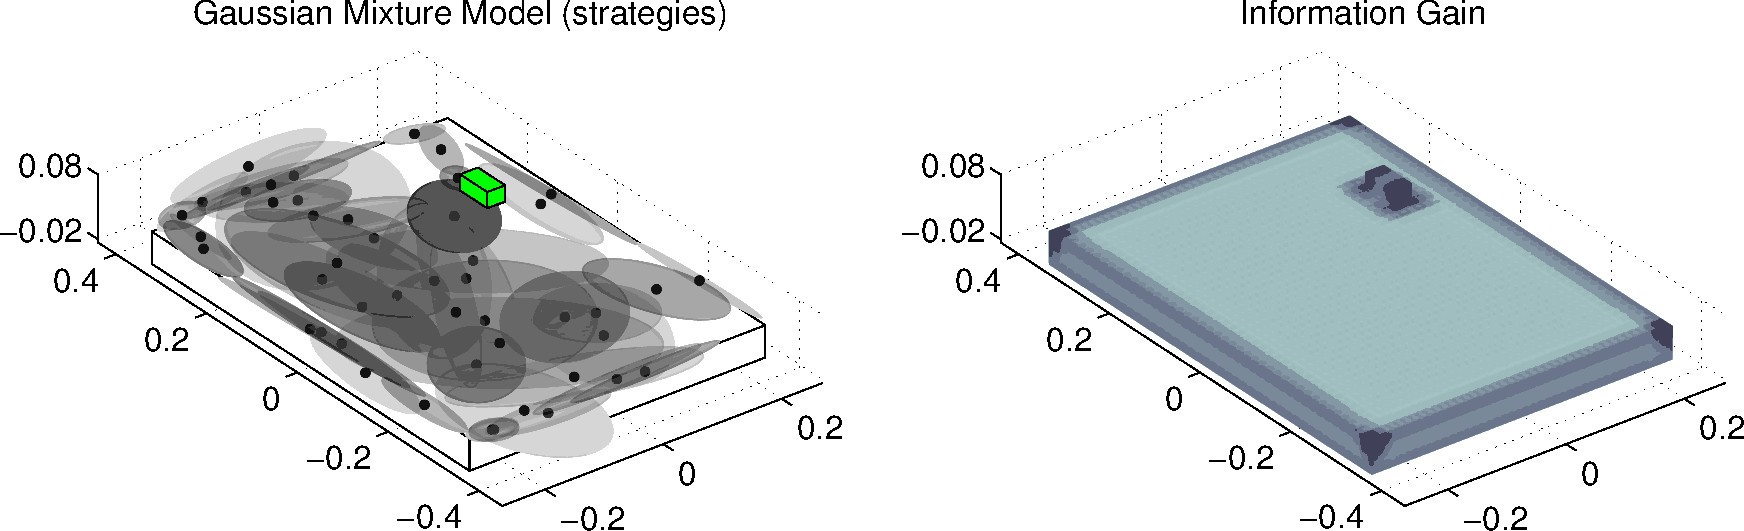
\includegraphics[width=0.95\textwidth]{./ch3-Search/Figures/Figure4}
  \caption{\textit{Left: } Resulting search GMM, a total of 67 Gaussian mixture components are present. We note the many overlapping Gaussians: this results
from the level of uncertainty over the different choices taken. For example humans follow along the edge of the table in different directions and might
leave the edge once they are confident with respect to their location. \textit{Right:} Information Gain map of the table environment, dark regions indicate 
high information gain as oppose to lighter ones. Not surprisingly, the highest are the corners, followed by the edges.}
  \label{fig:gmm}
\end{figure}

\subsection{Coastal Navigation}\label{chap3:costal_policy}

Coastal navigation \cite{CostalNavigation1999} is a path planning method in which the objective function, 
Equation \ref{eq:objective_function}, is composed of two terms.

\begin{equation}\label{eq:objective_function}
 f(x_{0:T}) = \sum\limits_{t=0}^{T} \lambda_1 \cdot c(x_t) + \lambda_2 \cdot I(x_t)
\end{equation}

The first term, $c(x_t)$, is the traditional ``cost to go'' which penalizes every step taken so as to ensure that the
optimal path is the shortest. The value was simply set to 1 for all discrete states in our case. The second term, $I(x_t)$, 
is the information gain of a state. The information gain, $I$, of a particular state is related to how much 
the entropy of a probability density function (pdf), being the location's uncertainty in our case, can be reduced. The two $\lambda$'s are scalars which weigh the influence 
of each term.

In our table environment we discretised the state space, $\mathbb{R}^3$, into bins so as to have a resolution of approximately, $1 cm^3$, giving us a total of a 125'000
states. The action space was discretised to 6 actions, two for each dimension meaning that all motion is parallel to the axis. For each state, $x_t$, an $I(x_t)$ value is
computed by evaluating Equation \ref{eq:IG},

% Explain how the Information Gain is computed

\begin{equation}\label{eq:IG}
 I(x_t) = \mathbb{E}_{p(y_t|x_t)}\{ H(p_{\Param}(x_t|y_{0:t},\dot{x}_{0:t}) \} - H(p_{\Param}(x_t|y_{0:t-1},\dot{x}_{0:t}))
\end{equation}
which is essentially the difference between the entropy of a prior pdf to that of a posterior pdf.
We set our initial pdf to be uniformly distributed and  we computed the maximum likelihood sensation for each discrete state $x_t$
which is akin to the expected sensation or assuming that there is no uncertainty in sensor measurement (an assumption 
often made throughout the literature to avoid carrying out the integral of the expectation in Equation \ref{eq:IG}).
The result is the difference between the posterior pdf, given that the sensation occurred in $x_t$, and the prior pdf. The resulting cost
map is illustrated in Figure \ref{fig:gmm}. As expected, corners have the highest information gain followed by edges and surfaces. 
We do not show the values of the table since they provided much less information gain.

The optimization of the objective function is accomplished by running the Dijkstra's algorithm. This algorithm, given a cost map, 
computes the shortest path to a specific target from all the states. This results in a policy.

\subsection{Control}
The standard approach to control with a GMM is to condition on the state,
$\hat{x}_t$ and $U_t$ in our case, and perform inference on the resulting conditional
GMM, Equation \ref{eq:conditional}, which is a distribution over velocities or directions.

\begin{equation} \label{eq:conditional}
  \pi_{\Param}(\dot{x}|\hat{x},U) = \sum\limits_{k=1}^{K} w^{k}_{\dot{x}|\hat{x},U} \;\;  g\left(\dot{x}\: ;  \MuK_{\dot{x}|\hat{x},U}, \SigK_{\dot{x}|\hat{x},U} \right)
\end{equation}

The new distribution is of the dimension of the output variable, the velocity (dimension 3). 
The variable $\dot{x}$ in $\dot{x}|\hat{x},U$ indicates the predictor variable and the variables $\hat{x},U$ have been conditioned.
A common approach in statistical PbD methods using GMMs is to take the expectation of the conditional (known as Gaussian Mixture Regression), equation \ref{eq:GMR}

\begin{equation} \label{eq:GMR}
 \dot{x} = \mathbb{E}\{\pi_{\Param}(\dot{x}|\hat{x},U)\} = \sum\limits_{k=1}^{K}  w^{[k]}_{\dot{x}|\hat{x},U} \; \MuK_{\dot{x}|\hat{x},U}
\end{equation}

The problem with this expectation approach, is that it averages out opposing directions or strategies and may leave 
a net velocity of zero. One possibility would be to sample from the conditional, however this can lead to non-smooth 
behaviour and flipping back and forth between modes resulting in no displacement. To maintain consistency between the
choices and avoid random switching  we perform a weighted expectation on the means so that 
directions (modes) similar to the current direction of the end-effector receive
a higher weight than opposing directions. For every mixture component $k$, a weight $\alpha_k$ is computed based 
on the distance between the current direction and itself.
If the current direction agrees with the mode then the weight remains unchanged but if it is in
disagreement a lower weight is
calculated according to the equation below. 
\begin{equation}  \label{eq:weight}
  \alpha_{k}(\dot{x}) = \piK_{\dot{x}|\hat{x},U} \; \exp(-\cos^{-1}(<\dot{x},\MuK_{\dot{x}|\hat{x},U}>))
\end{equation}
Gaussian Mixture Regression is then performed with the normalised  weights $\alpha$ instead of $\pi$
(the initial weight obtained when conditioning).

\begin{equation}\label{eq:w_expectation}
 \dot{x} = \mathbb{E}_{\alpha}\{\pi_{\Param}(\dot{x}|\hat{x},U)\} = \sum\limits_{k=1}^{K} \alpha_{k}(\dot{x}) \:\MuK_{\dot{x}|\hat{x},u}
\end{equation}
% 
%	How to control speed
%
The final output of equation \ref{eq:w_expectation} gives the desired direction
($\dot{x}$ is re-normalised). In the case when the mode suddenly disappears
(because of sudden change of the level of uncertainty caused by the appearance or disappearance of a feature)
another present mode is selected at random. For example, when the robot has reached a corner, the level of uncertainty for this feature drops to zero.
A new mode, and hence new direction of motion, will then  be computed.
However this is not enough to be able to safely control the robot.
One needs to control the amplitude of the velocity and ensure compliant control 
of the end-effector when in contact with the table. This behaviour is not learned here, as this is specific to 
the embodiment of the robot and unrelated to the search strategy. The 
amplitude of the velocity is computed by a proportional controller based on the
believed distance to the goal,
\begin{equation}
 \nu = \max(\min(\beta_{1},K_{p}(x_{\mathrm{g}} - \hat{x}),\beta_{2})
\end{equation}
where the $\beta$'s are lower and upper amplitude limits, $x_{g}$ is the
position of the goal, and $K_{p}$ the proportional gain which was tuned through
trials.

%
%	images/flow_chart.eps
%

\begin{figure}
\centering
  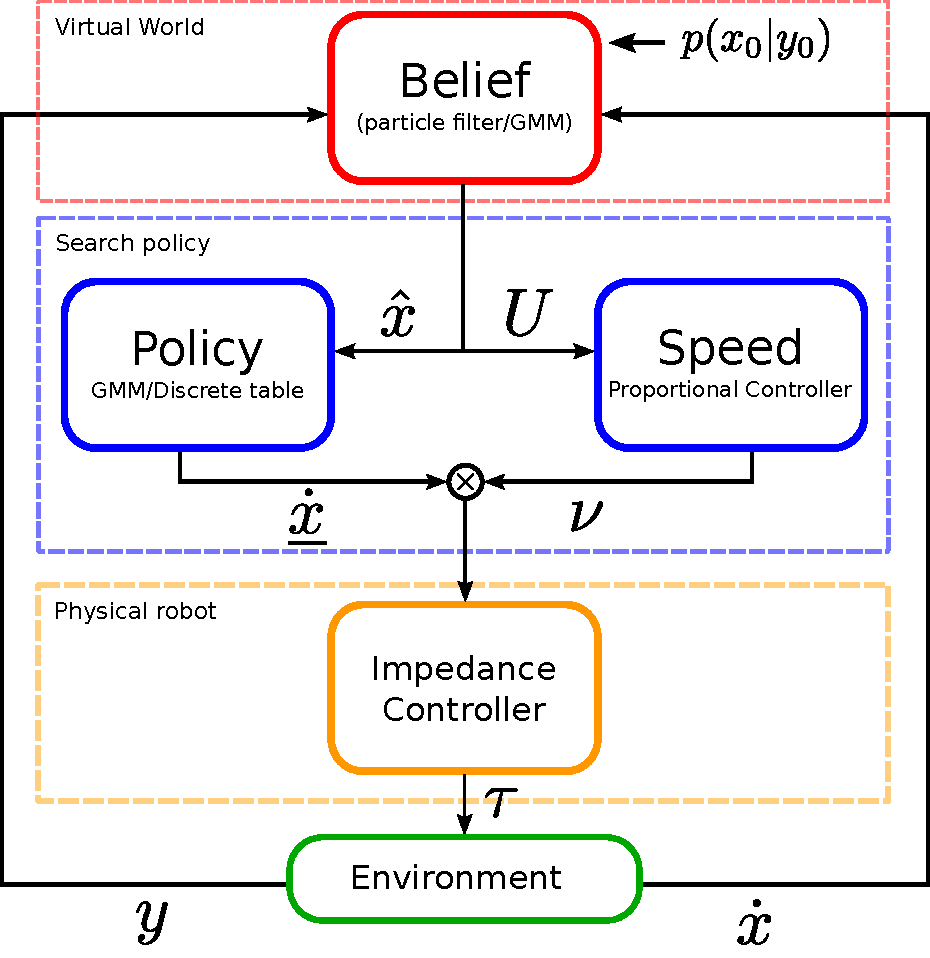
\includegraphics[width=0.8\textwidth]{./ch3-Search/Figures/Control_schematics}
  \caption{Overview of the decision loop. At the top a strategy is chosen given an initial belief
$p(x_{0}|y_{0})$ of the location of the end-effector (initially through sampling the conditional). 
A speed is applied to the given direction based on the believed distance
to the goal. This velocity is passed onwards to
a low level impedance controller which sends out the required torques. The
resulting sensation, encoded through the Multinomial distribution over
  the environment features, and actual displacement are sent back to update the
belief.}
  \label{fig:flow_chart}
\end{figure}

%
%	Impedance controller
%
As mentioned previously, compliance is the other important aspect when having the robot duplicate the search strategies. 
Collisions with the environment occur as a result of the uncertainty. To avoid risks of breaking the table or the robot sensors we have an impedance controller
at the lowest level which outputs appropriate joint torques $\tau$. The overall control loop is depicted in Figure \ref{fig:flow_chart}.



%%%%%%%%%%%%%%%%%%%%%%%%%%%%%%%%%%%%%%%%%%%%%%%%%%%%%%%%%%%%%%%%%%%%%%%%%%%%%%%%%%%%%%%%%%%%%%%%%%%%%%%%%%%%%%%%%%%%%%%%%%%%%%%%%%%%%%%%%
%																	   %
%				Results and Discussion  										   %
%																	   %
%%%%%%%%%%%%%%%%%%%%%%%%%%%%%%%%%%%%%%%%%%%%%%%%%%%%%%%%%%%%%%%%%%%%%%%%%%%%%%%%%%%%%%%%%%%%%%%%%%%%%%%%%%%%%%%%%%%%%%%%%%%%%%%%%%%%%%%%%
\FloatBarrier
\section{Results and discussion}\label{chap3:results}

Throughout our evaluation of our GMM PbD-POMDP control policy we will be considering four search policies: Greedy, GMM, Hybrid and 
Coastal. We evaluate behaviour present in the human demonstrations, and the four above mentioned policies in terms 
of their riskiness. We qualitatively compare the policies of the GMM model and the Coastal Navigation algorithm and highlight the 
effect of uncertainty. We finish with a quantitative evaluation of search efficiency in terms of distance travelled until the goal is found.
The layout of this section follows as:
\begin{itemize}
 \item Section \ref{sub:search_behaviour}, we analyse the types of behaviour present in the human demonstration as well as in
four different search algorithms: Greedy, GMM, Hybrid and Coastal.
 \item Section \ref{sub:policy_analysis}, we qualitatively analyse the GMM search policy (namely the different modes/decisions present) 
 with respect to the Coastal navigation policy.
 \item Section \ref{sub:time_uncertainty}, we evaluate the search performance, with respect to the distance taken to reach the goal and the uncertainty profiles towards the end of 
the searches in 5 different experiments (different types of initializations). 
\end{itemize}
\FloatBarrier
\subsection{Search \& behaviour analysis}\label{sub:search_behaviour}

For each method (Greedy, GMM, Hybrid, Coastal) 70 searches were performed with all starting positions drawn from the
uniform distribution used during the teaching stage (depicted in Figure \ref{fig:experiment} \textit{top right}, page \pageref{fig:experiment}). 
In Figure \ref{fig:expectedfeatures} we illustrate the expected sensation $\mathbb{E}\{y\}$ and  variance $\mathrm{Var}\{y\}$ for each trajectory with respect 
to the edge and corner of the table. 

\begin{figure}
  \centering
  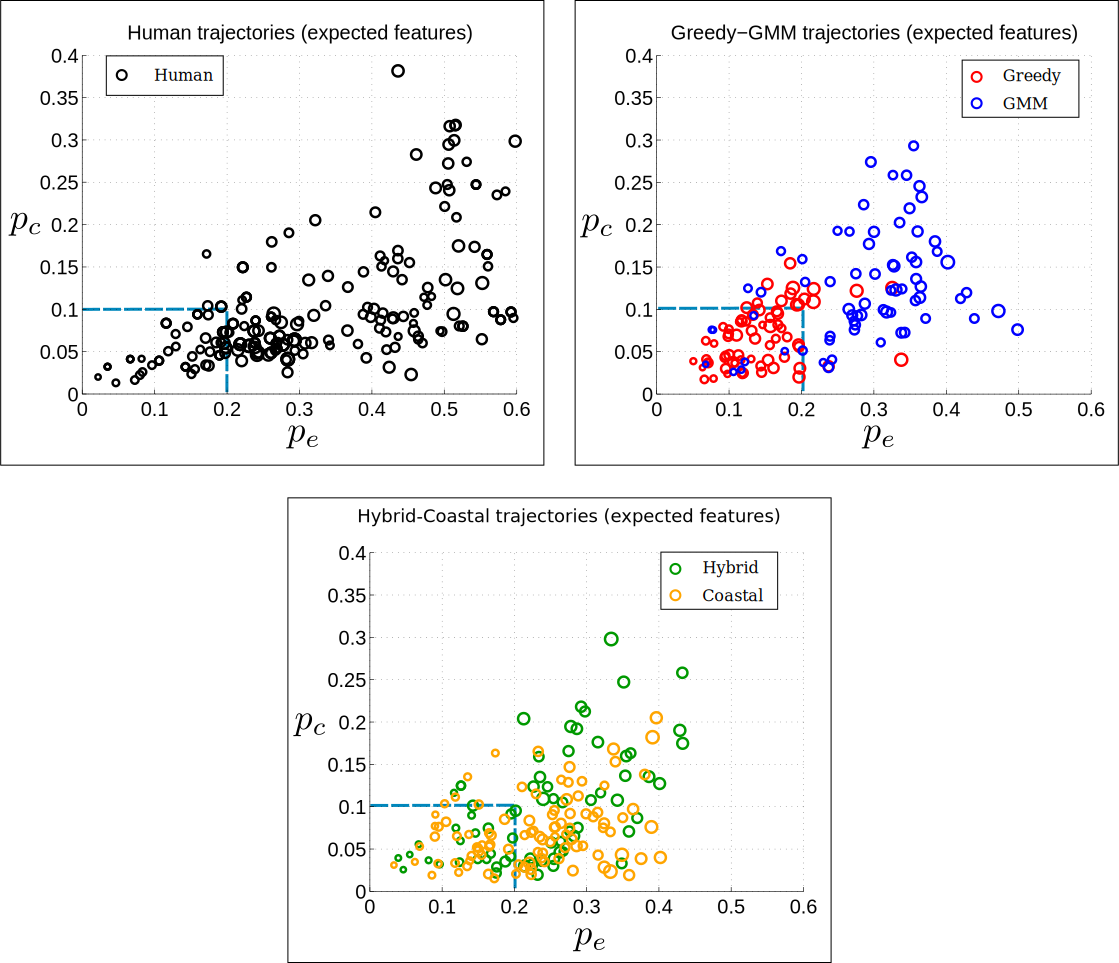
\includegraphics[width=\textwidth]{./ch3-Search/Figures/Figure6} 
  \caption{Expected sensation. Plots of the expected sensation of the edge and corner feature for all trajectories. 
  The axes are associated with the 
  sensor measurements, 0 means that the corresponding feature is not sensed and 1 the feature is fully sensed. 
  A point in the plots summarises a whole trajectory by the mean and variance of the probability of sensing a corner or edge. 
  The radius of the circles are proportional to the variance. The doted blue rectangle represents the decision boundary 
  for classifying a trajectory as being either risk-prone or risk-averse. A point which lies inside the rectangle is risk-prone.
  \textit{Left:} Human trajectories demonstrate a wide variety of behaviours ranging from those remaining close to features 
  to those preferring more risk. 
  \textit{Right:} Red points show Greedy and blue points the GMM model. 
  \textit{Bottom:} Green circles are associated with the Hybrid method whilst orange are those of the 
  Coastal navigation method. The Hybrid method is a skewed version of the GMM which tends towards risky behaviour and exhibits the 
  same kind of behaviour as the Coastal algorithm.}
  \label{fig:expectedfeatures}
\end{figure}


The selection of edges and corners as features as a means of classifying the type of behaviours present 
is not solely restricted to our search task. Salient landmarks will result in a high level of information
gain, which is the case for the edge and corner (see Figure \ref{fig:gmm} \textit{right}, page \pageref{fig:gmm}).
Other tasks can use such features or variants in which the curvature is considered for representing the task space. 
These features are present in most settings and high level features can use these easily as their building blocks.

We note that the Greedy search approach seeks to go directly to the goal without taking into account 
the uncertainty. The GMM models human search strategies. The Hybrid is a combination of both the Greedy and GMM method 
where once the uncertainty has been sufficiently minimised, the policy switches (threshold) to the Greedy method for the rest of 
the search. The Coastal navigation algorithm finds the optimal path to the goal based on an objective function which
consists of a trade-off between time taken to reach the goal and the minimisation of the uncertainty.

It can be seen that the human demonstrations have a much wider spread than those of the search algorithms. 
We suggest that this is due to human behaviours being optimal with respect to their own criteria as opposed to the algorithms 
which usually tend to only maximise a single objective function. The trajectories of the Greedy and GMM methods represented by their 
expected features demonstrate two distinctive behaviours (in terms of expected sensation), risk-prone for the Greedy and risk-adverse
for the GMM.

We make \textbf{the assumption} that Greedy trajectories are risk-prone by nature. We performed a SVM classification on the 
Greedy-GMM expected features (Figure \ref{fig:expectedfeatures} \textit{right}) and used the result to construct a decision boundary as a means
of classifying a trajectory as being either risk-prone or risk-averse. Table \ref{tab:percentage-risk-prone} \textit{first row} shows that
the GMM and Human search trajectories are mostly risk-averse. Surprisingly the Coastal policy seems to be very risk-prone given 
that it seeks paths close to highly informative areas.
We use a second metric based on the information gain, which we call the Risk factor, to classify trajectories as being either 
risk-prone or risk-averse.

The Risk factor of each individual trajectory is inversely proportional to its accumulated information gain. Figure \ref{fig:riskexamples} (\textit{left}) shows the kernel density estimation distribution of the risk 
for each search method. Two trajectories per search type corresponding to a supposed risk-prone and risk-averse search
are plotted in the expected feature space in Figure \ref{fig:riskexamples} (\textit{right}). As expected, risk-prone strategies 
for which the risk tends to 1 have a low expectation of sensing edges and corners and produce trajectories with a 
low information gain while those with a high expectation of sensing features have a high information gain. 
Since the metric lies exclusively in the range [0,1] we define that every trajectory which has a Risk factor lower than than 0.5 will 
be considered risk-averse whilst those above are risk-prone. Table \ref{tab:percentage-risk-prone} \textit{second row} illustrates
the riskiness of each search method. It is evident that humans are risk-averse in general followed by GMM which is a smoothing 
of the human data, then Hybrid which as expected should be more risk-prone since it is a linear interpolation between the GMM and 
Greedy search policies and finally Coastal and Greedy.

\begin{figure}
  \centering
  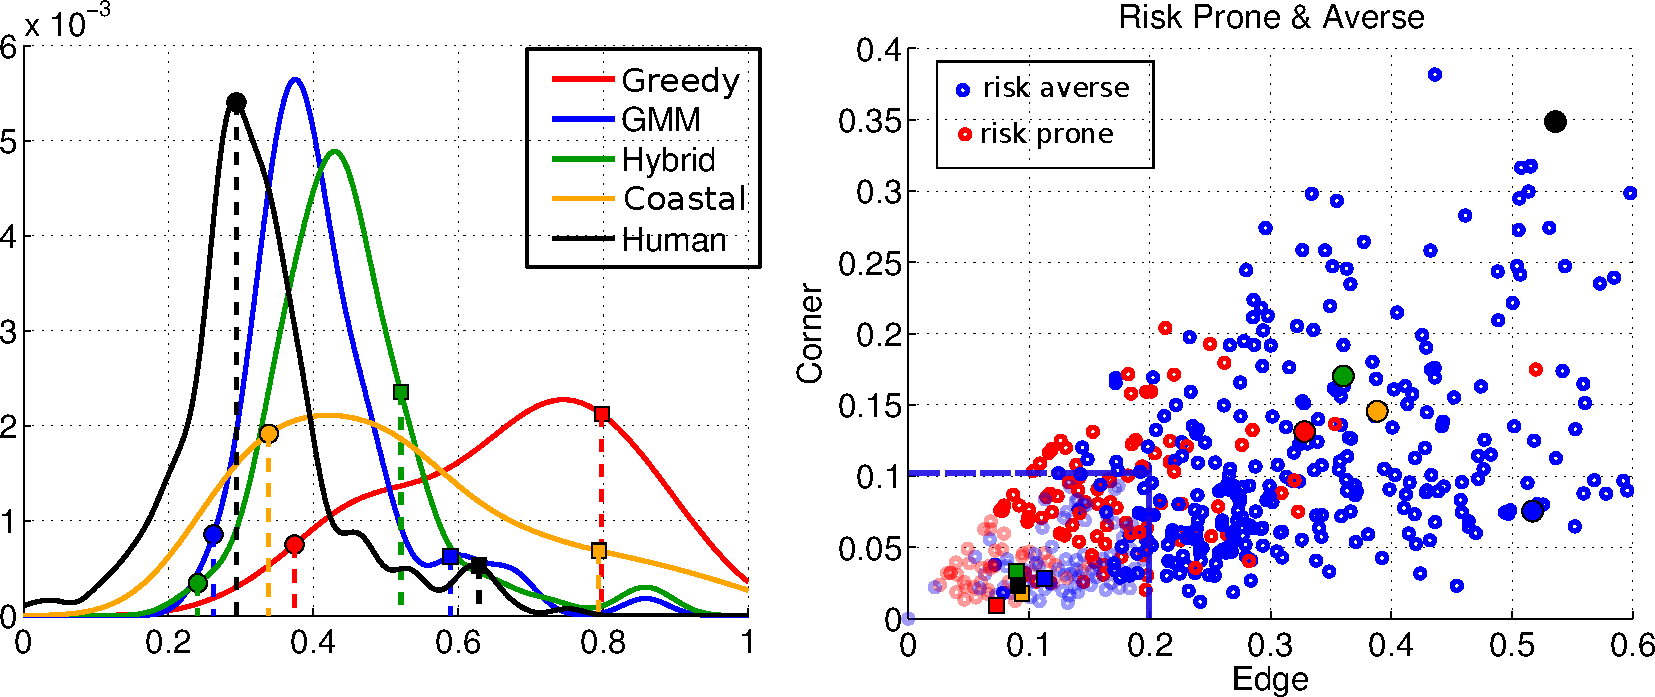
\includegraphics[width=\textwidth]{./ch3-Search/Figures/Figure7} 
 \caption{Risk of searches. Illustration of risk-prone and risk-averse searches in terms of a Risk factor (\textit{left}) and expected sensation (\textit{right}).
 \textit{Left:} Each trajectory was reduced to a single scalar, which we call the Risk factor, quantifying the risk of a trajectory. The Risk factor 
 is inversely proportional to the sum of the information gain of a particular trajectory. The colour paired dots (risk averse) and squares (risk prone) 
 represent trajectories which are plotted in 
 Figure \ref{fig:risk_examples}, to illustrate that these correspond to risk averse and prone searches.
 \textit{Right:} Corresponding trajectories chosen in the Risk factor space but represented in the feature space. As expected, trajectories with
 a high risk map to regions of low expected feature. However the transition from the Risk space to feature space is non-linear and will result in a different
 risk-level classification than the feature metric previously discussed.}
 \label{fig:riskexamples}
\end{figure}



\begin{table}
\centering
\begin{minipage}{\textwidth}
\centering
 \begin{tabular}{|l|c|c|c|c|c|}
 \cline{1-6}
   Criteria        &  \textbf{Greedy} & \textbf{GMM}  & \textbf{Hybrid} & \textbf{Coastal} & \textbf{Human} \\ \hline
  risk-prone (f) &   77 \% & 11 \% &  30 \% & 46 \% & 26  \% \\ \hline
  risk-prone (r) &   78 \% & 12 \% &  24 \% & 45 \% &  7 \% \\ \hline
 \end{tabular}
\end{minipage}
 \caption{Percentage of risk-prone trajectories based on two decision criteria, the feature (f) and the risk (r) (information gain) metrics discussed above.}
 \label{tab:percentage-risk-prone}
\end{table}

Figure \ref{fig:risk_examples} (\textit{top left \& right}), shows risk-prone (red) and 
averse (green) trajectories produced by human demonstrations and by the Greedy search. Both these extremes
correspond to our intuition that risk-averse trajectories tend to remain closer to features or areas of high information gain
as oppose to risk-prone searches. However to stress the case that humans have multiple search strategies 
present, we performed 40 GMM searches (model of the human behaviour) which all started under the same initial conditions
(same belief distribution, true position and believed position). Figure \ref{fig:risk_examples}
shows the resulting trajectories and expected features for each trajectory. 
It is clear that multiple searches occur which is reflected in the plot of the expected features. All of the 
search strategies generated by the GMM for this initial condition produced risk-averse trajectories.


We conclude that there is a strong inclination towards inferring that indeed multiple search strategies do 
arise in the human searches since they were extracted and encoded in the GMM model. From the risk distribution, humans have a 
tendency to be risk-averse.

\begin{figure}
 \centering
  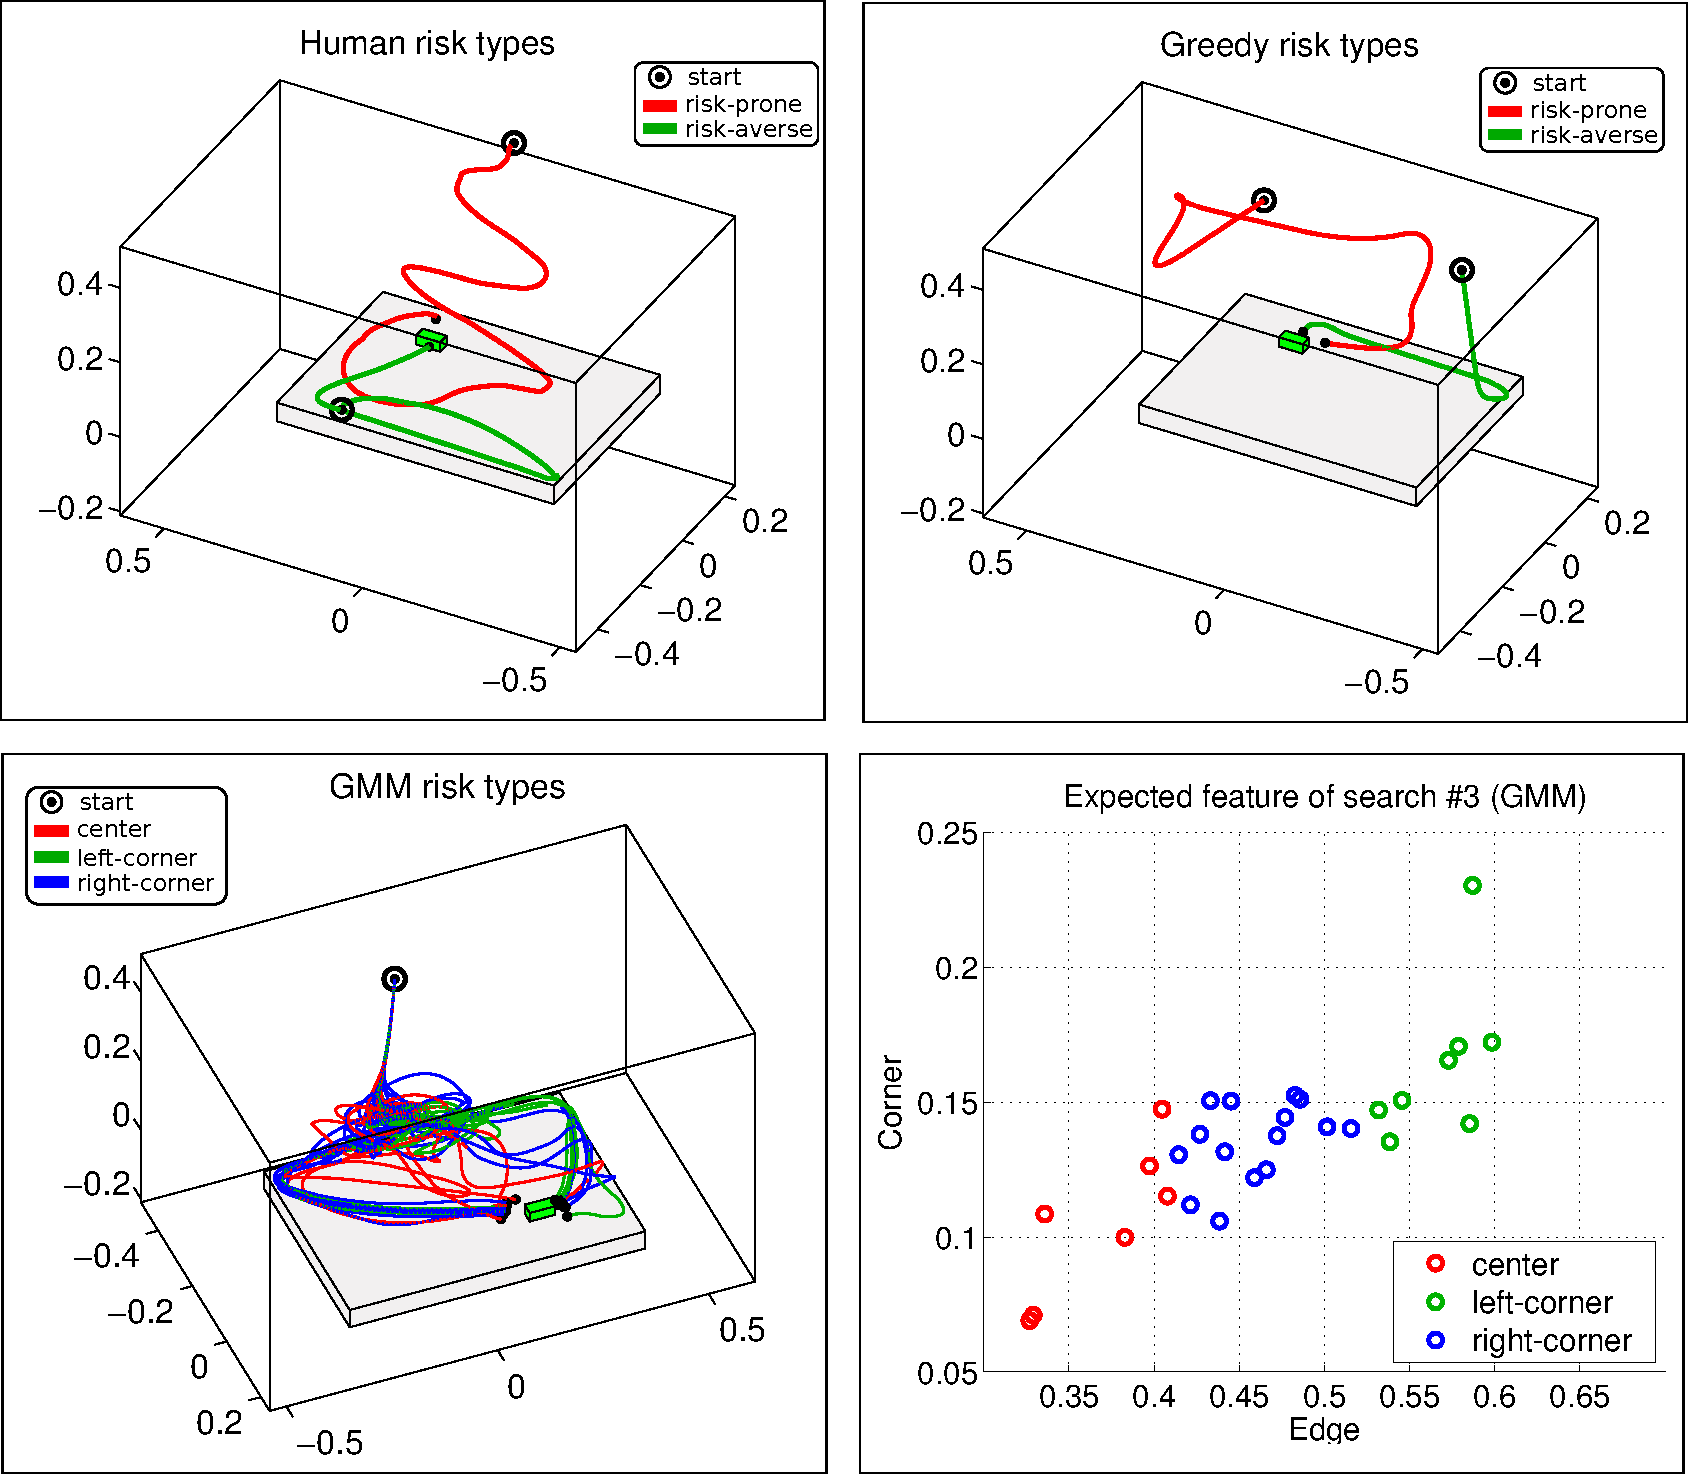
\includegraphics[width=0.95\textwidth]{./ch3-Search/Figures/Figure8}
  \caption{Risk prone \& averse searches (red \& green trajectories). \textit{Top left:}
  Two human trajectories taken from data shown in Figure \ref{fig:riskexamples}. 
  \textit{Top right:} Two Greedy trajectories. \textit{Bottom left:} GMM trajectories, all starting from the same location, the
  colour coding is to illustrate the different policies which were encoded and emerge given the same initial conditions. 
  \textit{Bottom right:} Corresponding expected features of each trajectory, the colour coding matches the trajectories 
  to the ``GMM risk types'' sub-figure. All the searches which were generated by the GMM for this initialisation produced
  risk-averse searches (based on the feature metric discussed previous).}
  \label{fig:risk_examples}
\end{figure}

\FloatBarrier
\subsection{GMM \& Coastal Navigation policy analysis}\label{sub:policy_analysis}

We next illustrate some of the modes (action choices) present during simulation and evaluate their 
plausibility. Figure \ref{fig:modes} shows that multiple decision points have been correctly embedded in the GMM model. All
arrows (red) indicate directions that reduce the level of uncertainty. 

\begin{figure}
    \centering
    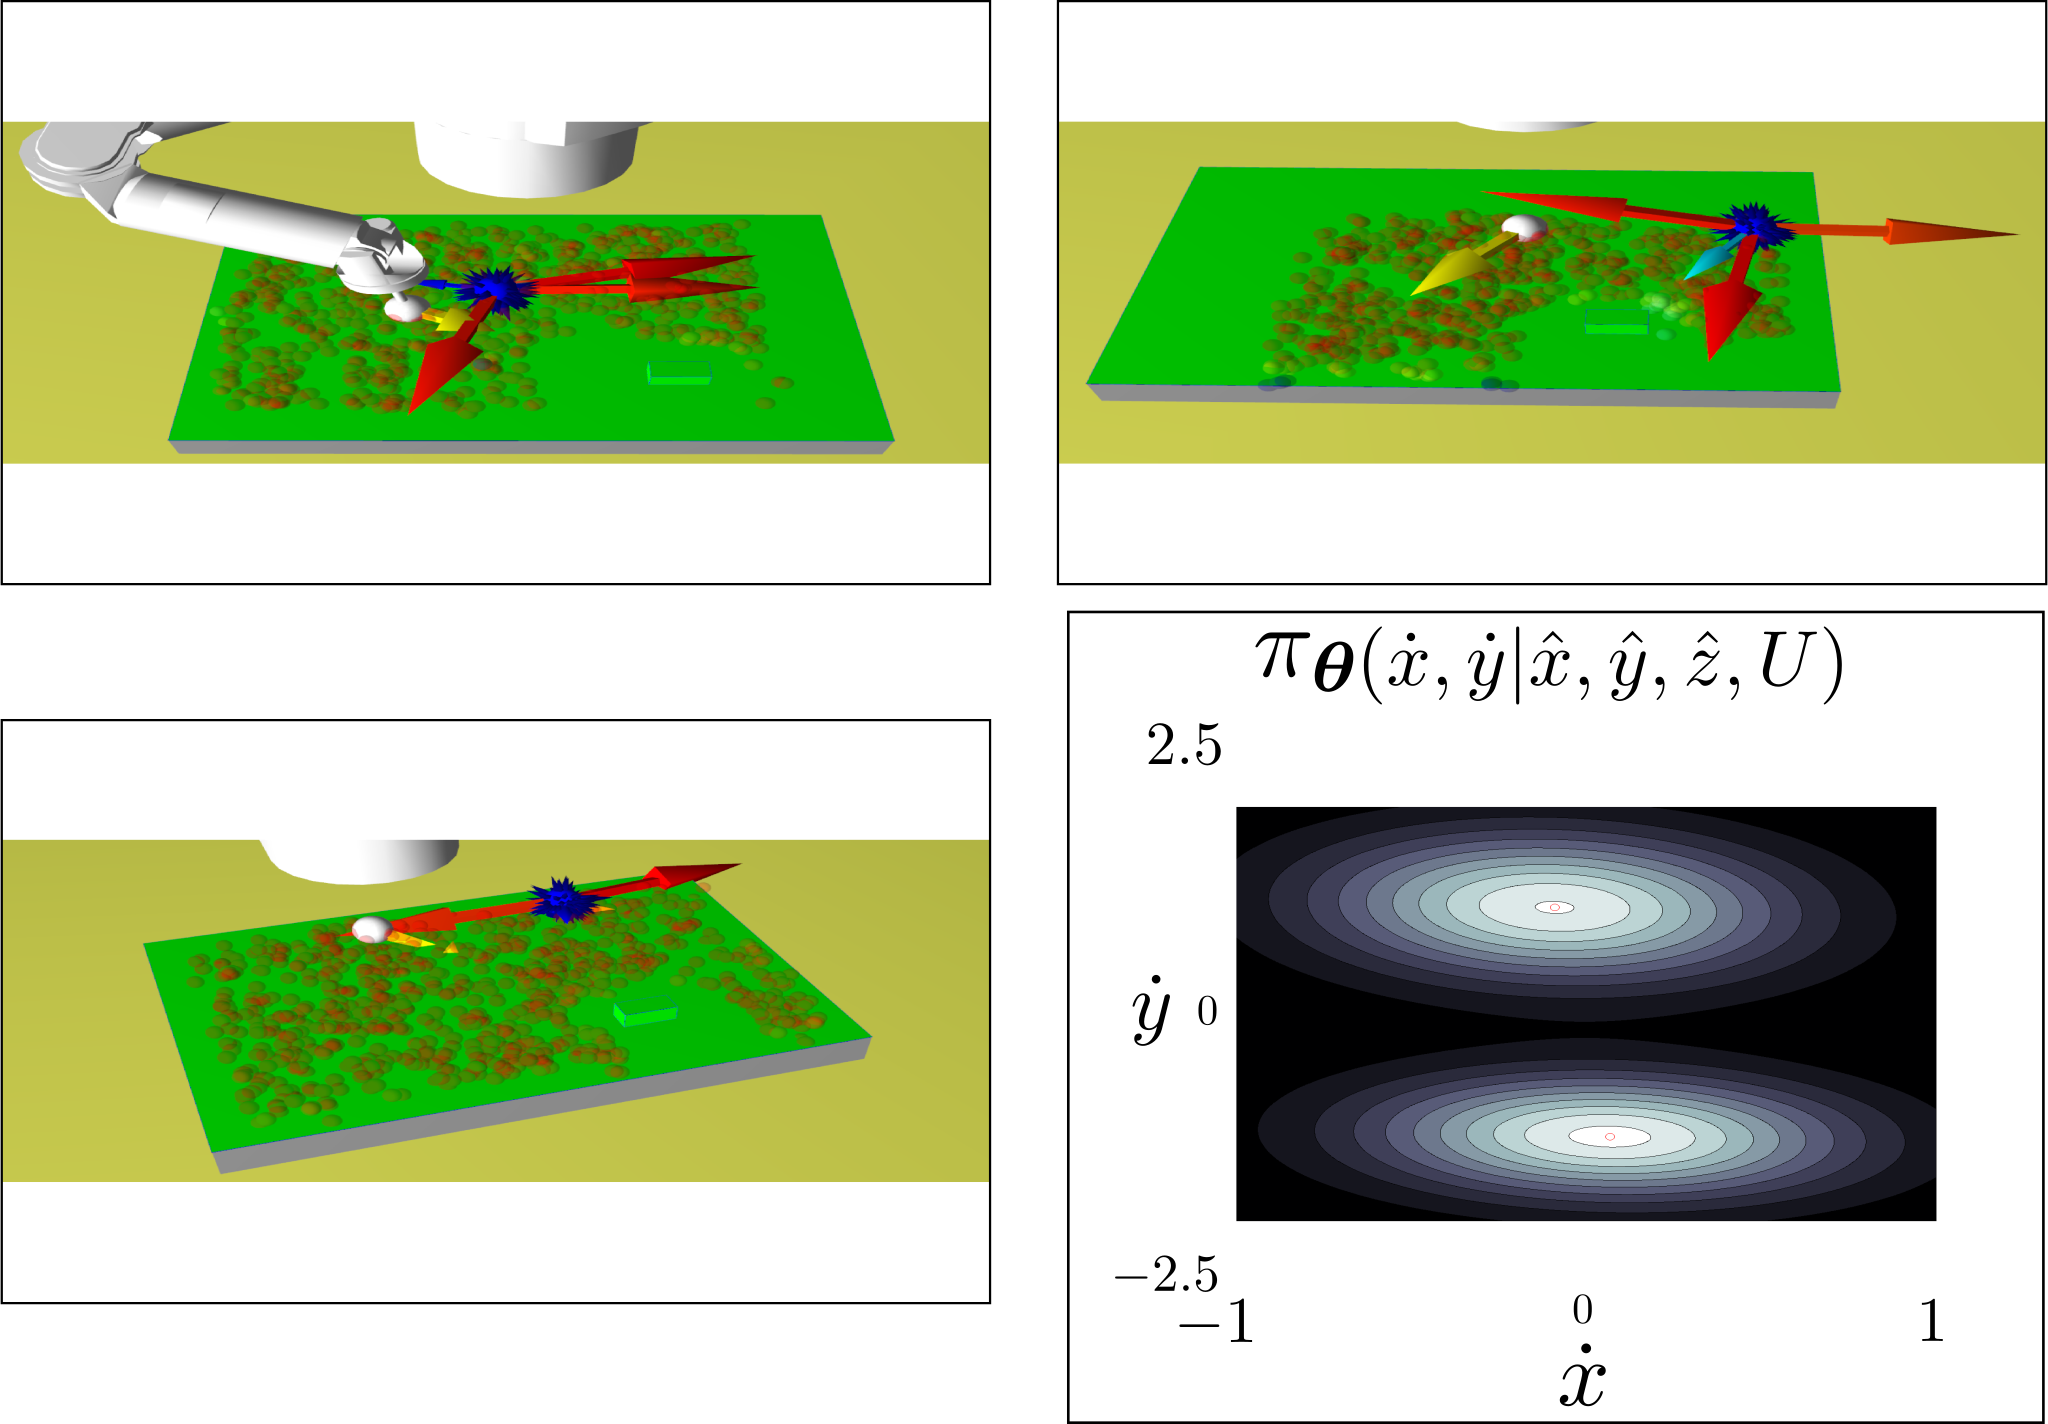
\includegraphics[width=0.95\textwidth]{./ch3-Search/Figures/Figure9_m}
    \caption{Illustration of three different types of modes present during the
    execution of the task where the robot is being controlled by the learned GMM model.
    The white ball represents the actual position of the robot's end-effector. The blue ball represents the
    believed position of the robot's end-effector and the robot is acting according to it. 
    The blue ball arrows represent modes. Colours encode the mode's weights given by the priors $\pi_{k}$ after conditioning ( but not re-weighted as
    previously described). The spectrum ranges from red (high weight) to blue (low weight). \textit{Top left:} Three modes are present, but two agree with each other.   
    \textit{Top right:} Three modes are again present indicating appropriate ways to reduce the uncertainty. \textit{Lower left:} Two modes are in opposing directions. 
    No flipping behaviour between modes occurs since preference is given to the modes pointing in the same direction as the robot's current trajectory. \textit{Lower right:} GMM modes when conditioned on the state represented in the lower left figure.
    The two modes represent the possible directions (un-normalised).}
   \label{fig:modes}
\end{figure}

Figure \ref{fig:vectorfield} depicts the vector fields of both Coastal and GMM models where, as expected, the Coastal navigation 
trajectories tend to stay close to edges and corners until they are sufficiently close to the goal. This is achieved by weighting 
the information gain term $I(x_t)$ in the objective function sufficiently ($\lambda_2$). If $\lambda_2$=0 the Coastal policy is 
the same Greedy algorithm. 

It can be further seen that when the uncertainty tends towards it's maximum value ($U \rightarrow 1$) 
all behaviour tends to go towards the edges and corners. As the uncertainty reduces ($U \rightarrow 0$) the vector field 
tends directly towards the goal. However even at a low level of uncertainty, the behaviour at the edges and corners remains 
multi-modal and tends to favour remaining close to the edges and corners. 
This is an advantage of the GMM model. If the uncertainty has been sufficiently reduced and 
the true position of the end-effector or hand is not near an 
edge the policy dictates to go straight to the goal. This is not the case for the Coastal algorithm which ignores the 
uncertainty and strives to remain in the proximity of corners and edges until sufficiently close. 
This approach could potentially lead to unnecessary travel cost which could otherwise have been avoided.

\begin{figure}
  \centering
  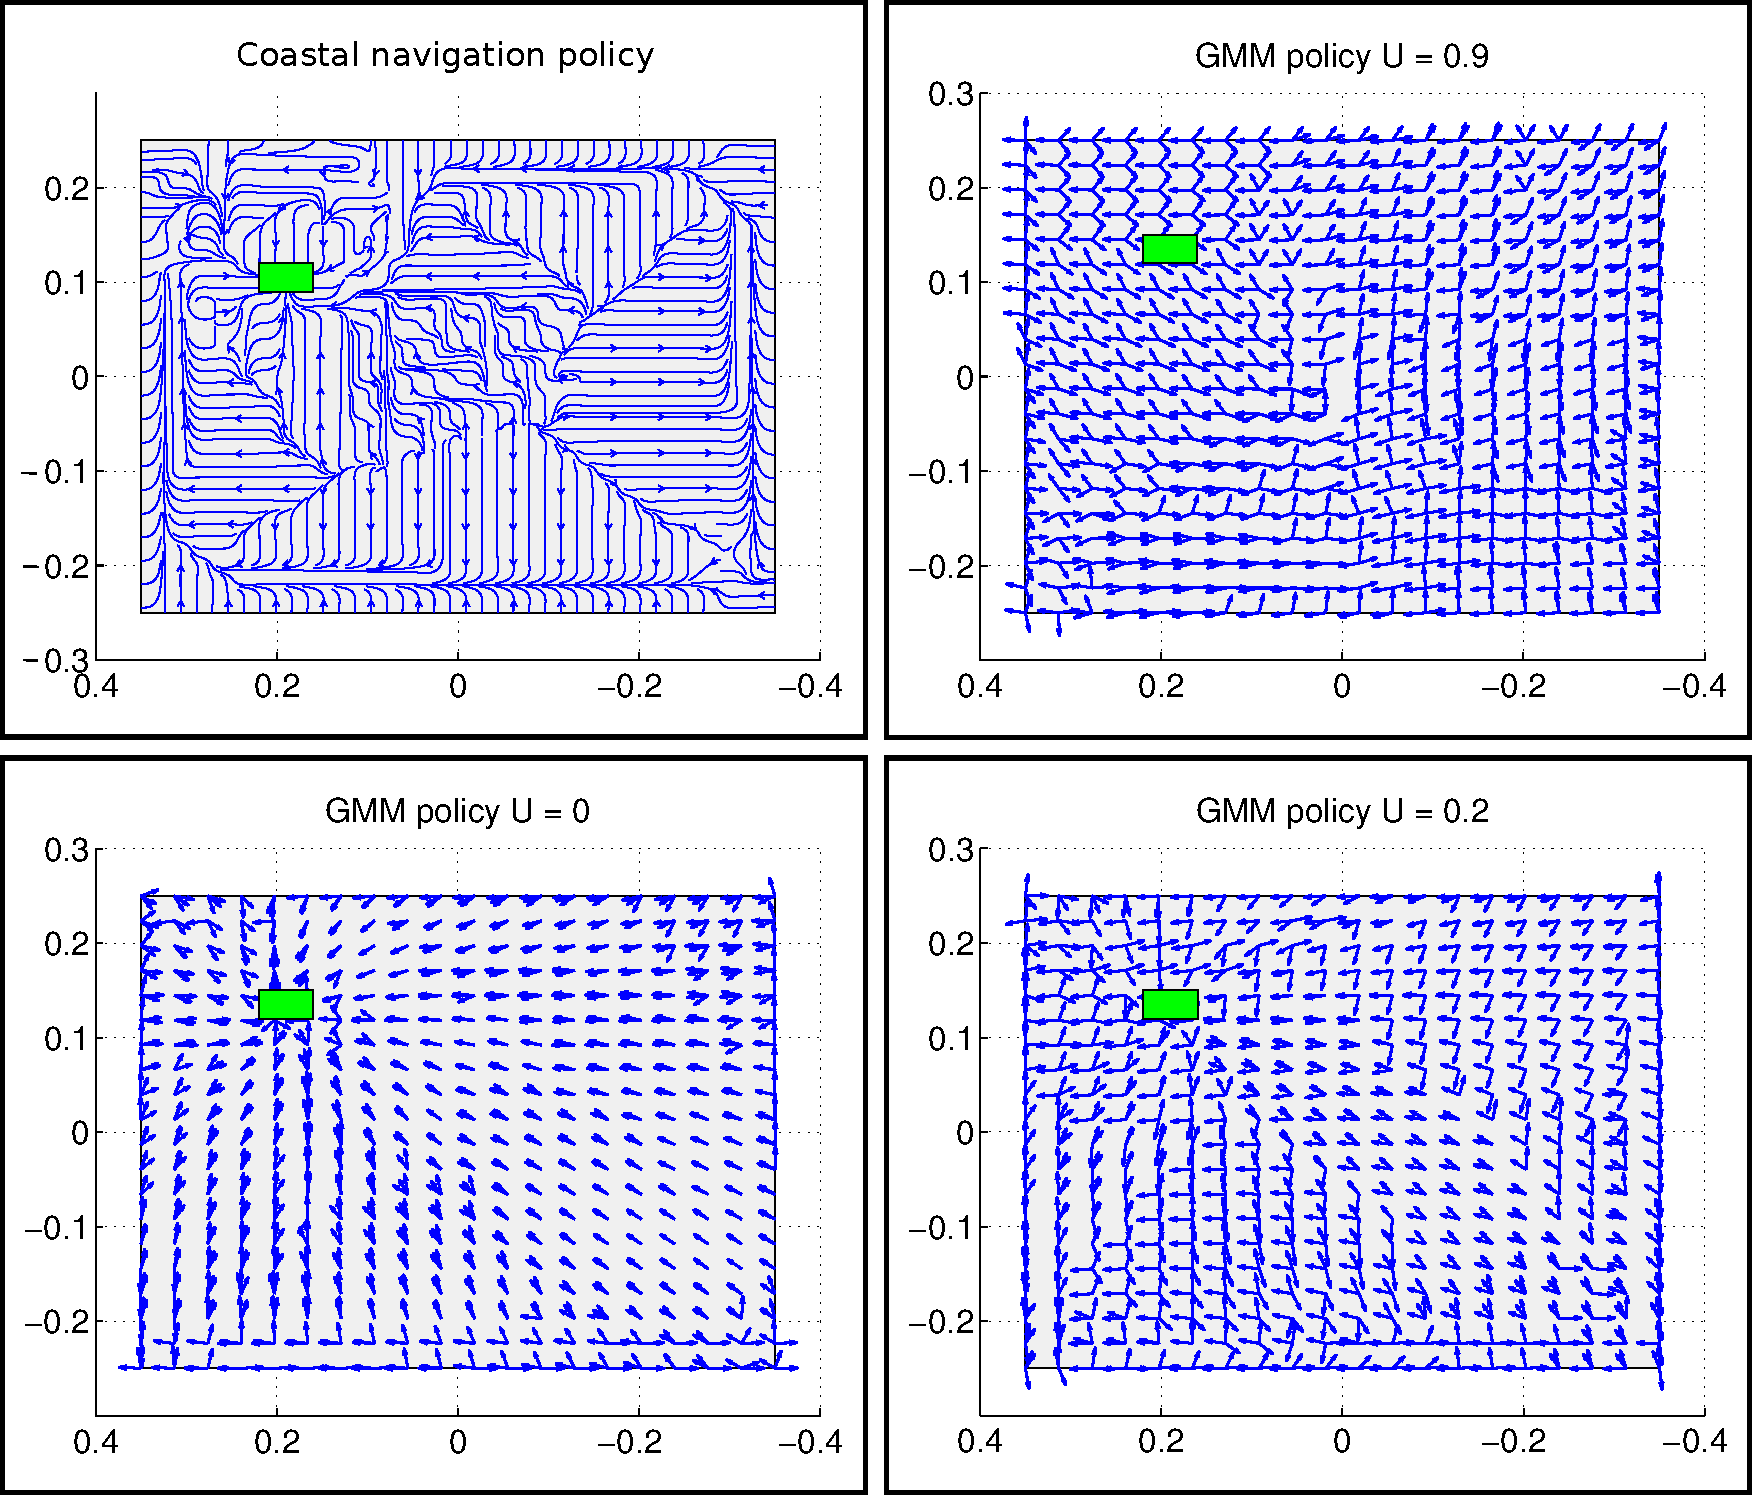
\includegraphics[width=0.95\textwidth]{./ch3-Search/Figures/Figure10}
  \caption{Illustration of the vector field for the Coastal and GMM policy. \textit{Top Left} Coastal policy, there is only one possible direction for every 
  state at any time, the values of $\lambda_2$ in the cost function were set experimentally. \textit{Others:} The GMM policy for three different levels of
  uncertainty. For each point multiple actions are possible which is reflected by the number of arrows (only the first three most likely actions). As 
  the uncertainty decreases the policy becomes less multi-model, but remains around the edges and corners. Note that once certain
  of being close to an edge there is a possibility to go either straight to the goal or stay close to the edge and corners.}
  \label{fig:vectorfield}
\end{figure}

\FloatBarrier
\subsection{Distance efficiency \& Uncertainty}\label{sub:time_uncertainty}

We seek to distinguish the most efficient method in terms of two metrics, the distance (in meters) taken to reach the goal
and the level of uncertainty upon arriving at the goal. We report results on 5 different search 
experiments in which we compare the Greedy, GMM and Coastal Navigation algorithms. The Hybrid was not fully considered since it 
is a heuristic combination of the Greedy and GMM methods. 

In the first experiment, the true and believed locations of the end-effector 
were drawn uniformly from the original start distribution (Figure \ref{fig:experiment}, \textit{top right}) 
reflecting the default setting. The initializations (both real and believed end-effector locations) for the 
remaining 4 experiments were chosen in order to reflect particular situations which highlight the differences 
and drawbacks between each respective search method.
For the first experiment (Uniform search experiment), a 100 trials were carried out in which the end-effector position and belief were 
initialized uniformly. As for the other 4 search experiments, 40 separate runs were carried for each of the three algorithms.

\begin{figure}
   \centering
 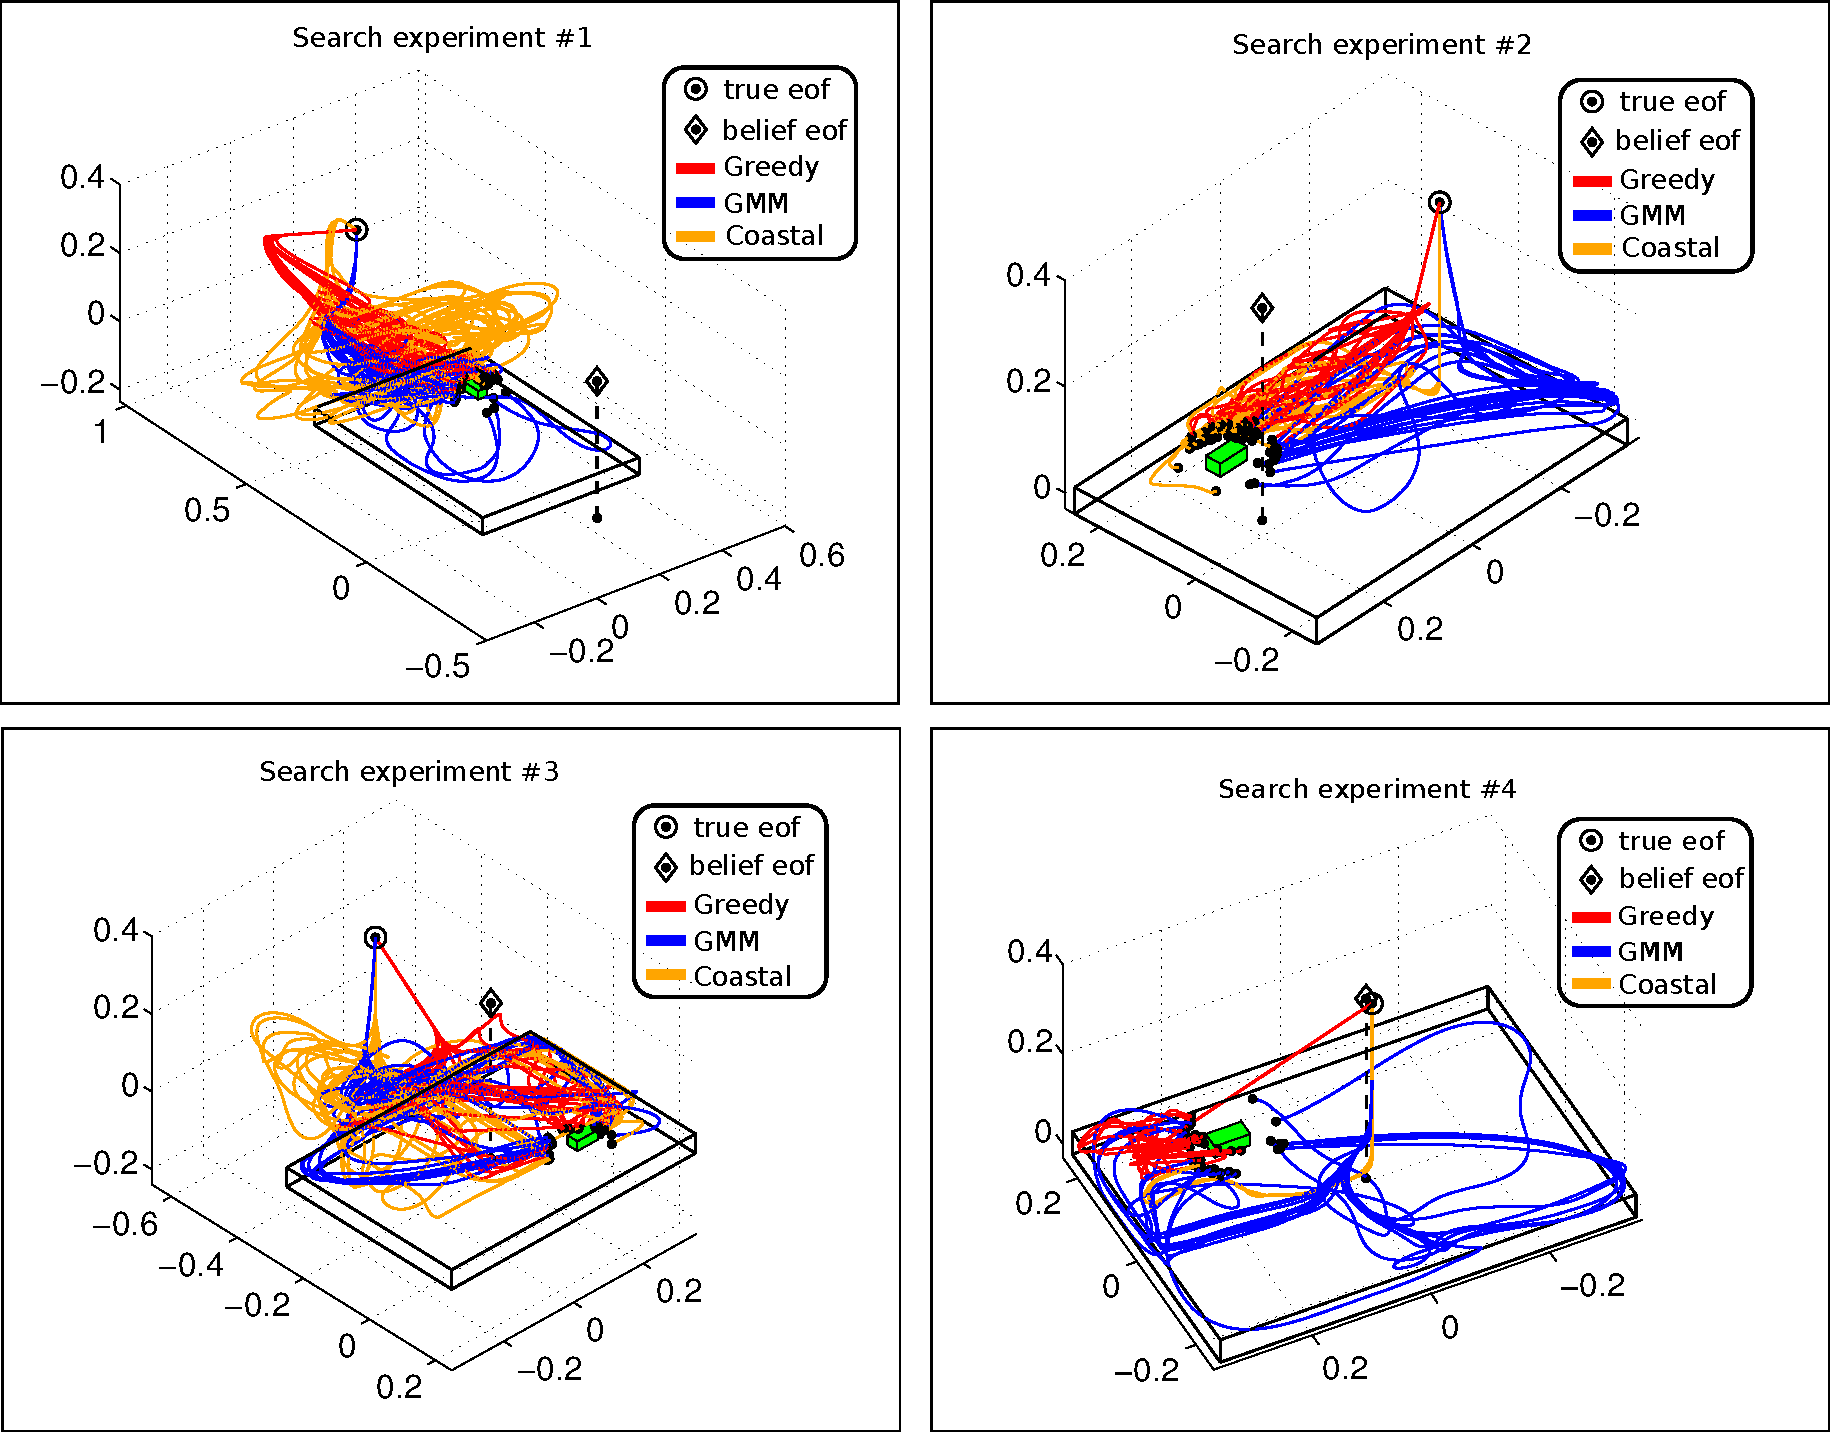
\includegraphics[width=\textwidth]{./ch3-Search/Figures/Figure11}
\caption{Four search initializations, from \textit{top left} to \textit{bottom right} we refer to them as \#1-4. The 
circle indicates the true starting point of the end-effector (eof), whilst the triangle is the initial believed location of the eof.
The initialisation in \#1 was chosen such that the true and believed eof locations were at opposite sides of the table. 
This setting was selected to highlight the draw back in methods which do not take into account uncertainty. 
The second initialisation \#2, reflects the situation where once again there is a large distance between true and believed location of 
the eof. However this time both are above the table. The starting points in \#3 are a variant on \#1 
with the difference being that the believed eof position is above the table whilst the true eof location is not. The last 
experiment \#4 was a setup which would be favourable to algorithms that are inclined to be greedy. Both true and believed 
eof locations are close to one another.}
\label{fig:four-initialisations}
\end{figure}

Table \ref{tab:mean-var-distance} reports the mean and variance of the distance taken (in meters) to reach the goal for each search 
method for all 5 experiments.
We report on an Analysis of Variance (ANOVA) to test that all experiments were 
significantly different from one another as were the searches. We test the null hypothesis,  $H_o$,  that there is 
no statistical difference between the 5 search experiments. 
Before performing the ANOVA, we verified that our dependent variable, distance [m] taken to reach the goal, follows a normal 
distribution for all methods and all experiments (a total of $5 \times 3 = 15$ tests), an assumption which is required by 
an ANOVA analysis. A Kolmogorov-Smirnov test was performed on each experiment and associated search method. A total 
of 11/15 searches rejected the null hypothesis with a significance level of less than 5\% (p-value $<$ 0.05). 

\begin{table}
 \centering
  \begin{tabular}{|c|c|c|c|c|}     
  \hline
      Experiment       &  \textbf{Greedy}      	  	&  \textbf{GMM}      		&  \textbf{Coastal}     \\\hline
       Uniform         &   1.54 (0.46) 	  		& 0.99 (0.14) \cellcolor{Gray} 	& 1.13 (0.57)    \\
	\#1            &   3.02 (0.36)    		& 1.82 (0.23) \cellcolor{Gray} 	& 3.44 (1.50)    \\
	\#2            &   0.80 (0.01) \cellcolor{Gray} & 1.41 (0.14) 			& 0.94 (0.01)    \\
	\#3            &   1.14 (0.08) \cellcolor{Gray} & 1.80 (0.17) 			& 2.14 (0.81)    \\
	\#4            &   0.75 (0.04)  		& 1.34 (0.07) 			& 0.68 (0.01) \cellcolor{Gray} \\ \hline
 \end{tabular}
  \caption{Mean distance and (variance) taken to reach the goal for 3 methods in 5 experiments. The grey shaded entries correspond to the results of the search algorithm 
  which obtained the fastest time to reach the goal in each type of experiment/search.}
  \label{tab:mean-var-distance}
\end{table}

In Table \ref{tab:anova-1} we report the p-values and F-statistics for an ANOVA on the 5 different experiments where our 
null hypothesis is that all experiments produce statistically the same type of search. For all experiment types the p-value 
is extremely small, below a significance value of 1\% (p-value $<$ 0.01) which indicates that we can safely reject the 
null hypothesis and accept that all experiments produced very different searches, which is important for a 
comparative study.

\begin{table}
 \centering
  \begin{tabular}{|c|c|c|c|c|c|}
  \hline
   search method &  Uniform       &   \#1	   & 	\#2	     & 	    \#3	       &   \#4 \\ \hline
   p-value (F)   &  2e-06 (14) & 5e-07 (19) &  7e-11 (36) &  4-06 (15) &  4e-16 (67) \\ \hline
 \end{tabular}
 \caption{ANOVA tests the null hypothesis that all search experiments produced the same type of search with respect to the distance taken to reach the goal. 
 All the p-values are extremely small which indicate that the null hypothesis can safely be rejected.}
 \label{tab:anova-1}
\end{table}

As the first ANOVA only indicated that the experiments produced different searches,
we also performed a second ANOVA test between the paired search methods to confirm that the methods themselves are statistically different.
Table \ref{fig:anova-2} illustrates the difference between the individual search methods for each experiment. 
It was found that most search algorithms produced significantly different searches (p-value $<$ 0.01) with
the exception of the GMM and Coastal algorithm for the Uniform and \#3 experiment (p-value $<$ 0.1). 
However the GMM and Coastal trajectories for the \#3 experiment appear to be quite different when the trajectories 
are off the table's surface, see Figure \ref{fig:four-initialisations} \textit{(Bottom left)}, but share similar 
characteristics such as edge following behaviour.

\begin{table}
 \centering
 \begin{tabular}{|c|c|c|c|}
 \hline
   p-value (F)   &  Greedy vs GMM      &     Greedy vs Coastal        &  GMM vs Coastal     \\\hline
  Uniform & 3.59e-08 (30)  &   3.32e-04 (13) 		     &  1.90e-01 (2)  \cellcolor{Gray}\\
\#1  	  & 5.80e-08 (46) &  1.88e-01 (2) \cellcolor{Gray} &  4.58e-06 (28)\\
\#2	  & 3.60e-08 (47) &  4.68e-04 (14)		    &  4.54e-06 (28) \\
\#3	  & 3.57e-07 (37) &  2.07e-05 (23)		    &  1.25e-01 (2) \cellcolor{Gray} \\
\#4	  & 6.70e-10 (64) &  1.58e-01 (2) \cellcolor{Gray} &  6.34e-13 (107) \\ \hline
\end{tabular}
\caption{ANOVA between paired search methods. The first column gives an indication of the probability that both the Greedy 
and GMM searches are statistically the same (the null hypothesis). This was rejected with a tolerance of below \%1. 
In the second column, Greedy vs Coastal searches \#1 and \#4 are statistically closer 
than the rest with a p-value threshold of 10\% required to be able to reject the null hypothesis. 
In the third column the uniform and \#3 are not statistically different and would require a higher threshold on the p-value to be so.}
\label{fig:anova-2}
\end{table}

From our ANOVA analysis we conclude that the behaviour exhibited by the three search strategies is 
significantly different. This is certainly the case for the Greedy and GMM methods, even though in 
certain situations the Greedy and Coastal policies display similar behaviour such as in experiment \#1.
The reason for this is that both the Greedy and Coastal policies start in a situation where there are no salient features available
and their polices take the true end-effector location to an even more feature deprived 
region. In this situation the GMM policy is the clear winner with respect to the distance taken to reach
the goal. 

In experiment \#2, both Greedy and Coastal policies perform equally well and will usually perform faster than the GMM model if the true 
and believed locations of the end-effector remain on the surface of the table. Otherwise if this is not the 
case, they will both reduce the uncertainty in a very inefficient way as the modes will often change during the search. 
This leads to the believed position (most likely state, $\hat{x}_t$) varying greatly, resulting in an increased time before the uncertainty 
has been narrowed down sufficiently for a contact to occur with the table (or simply by chance).


\begin{figure}
   \centering
  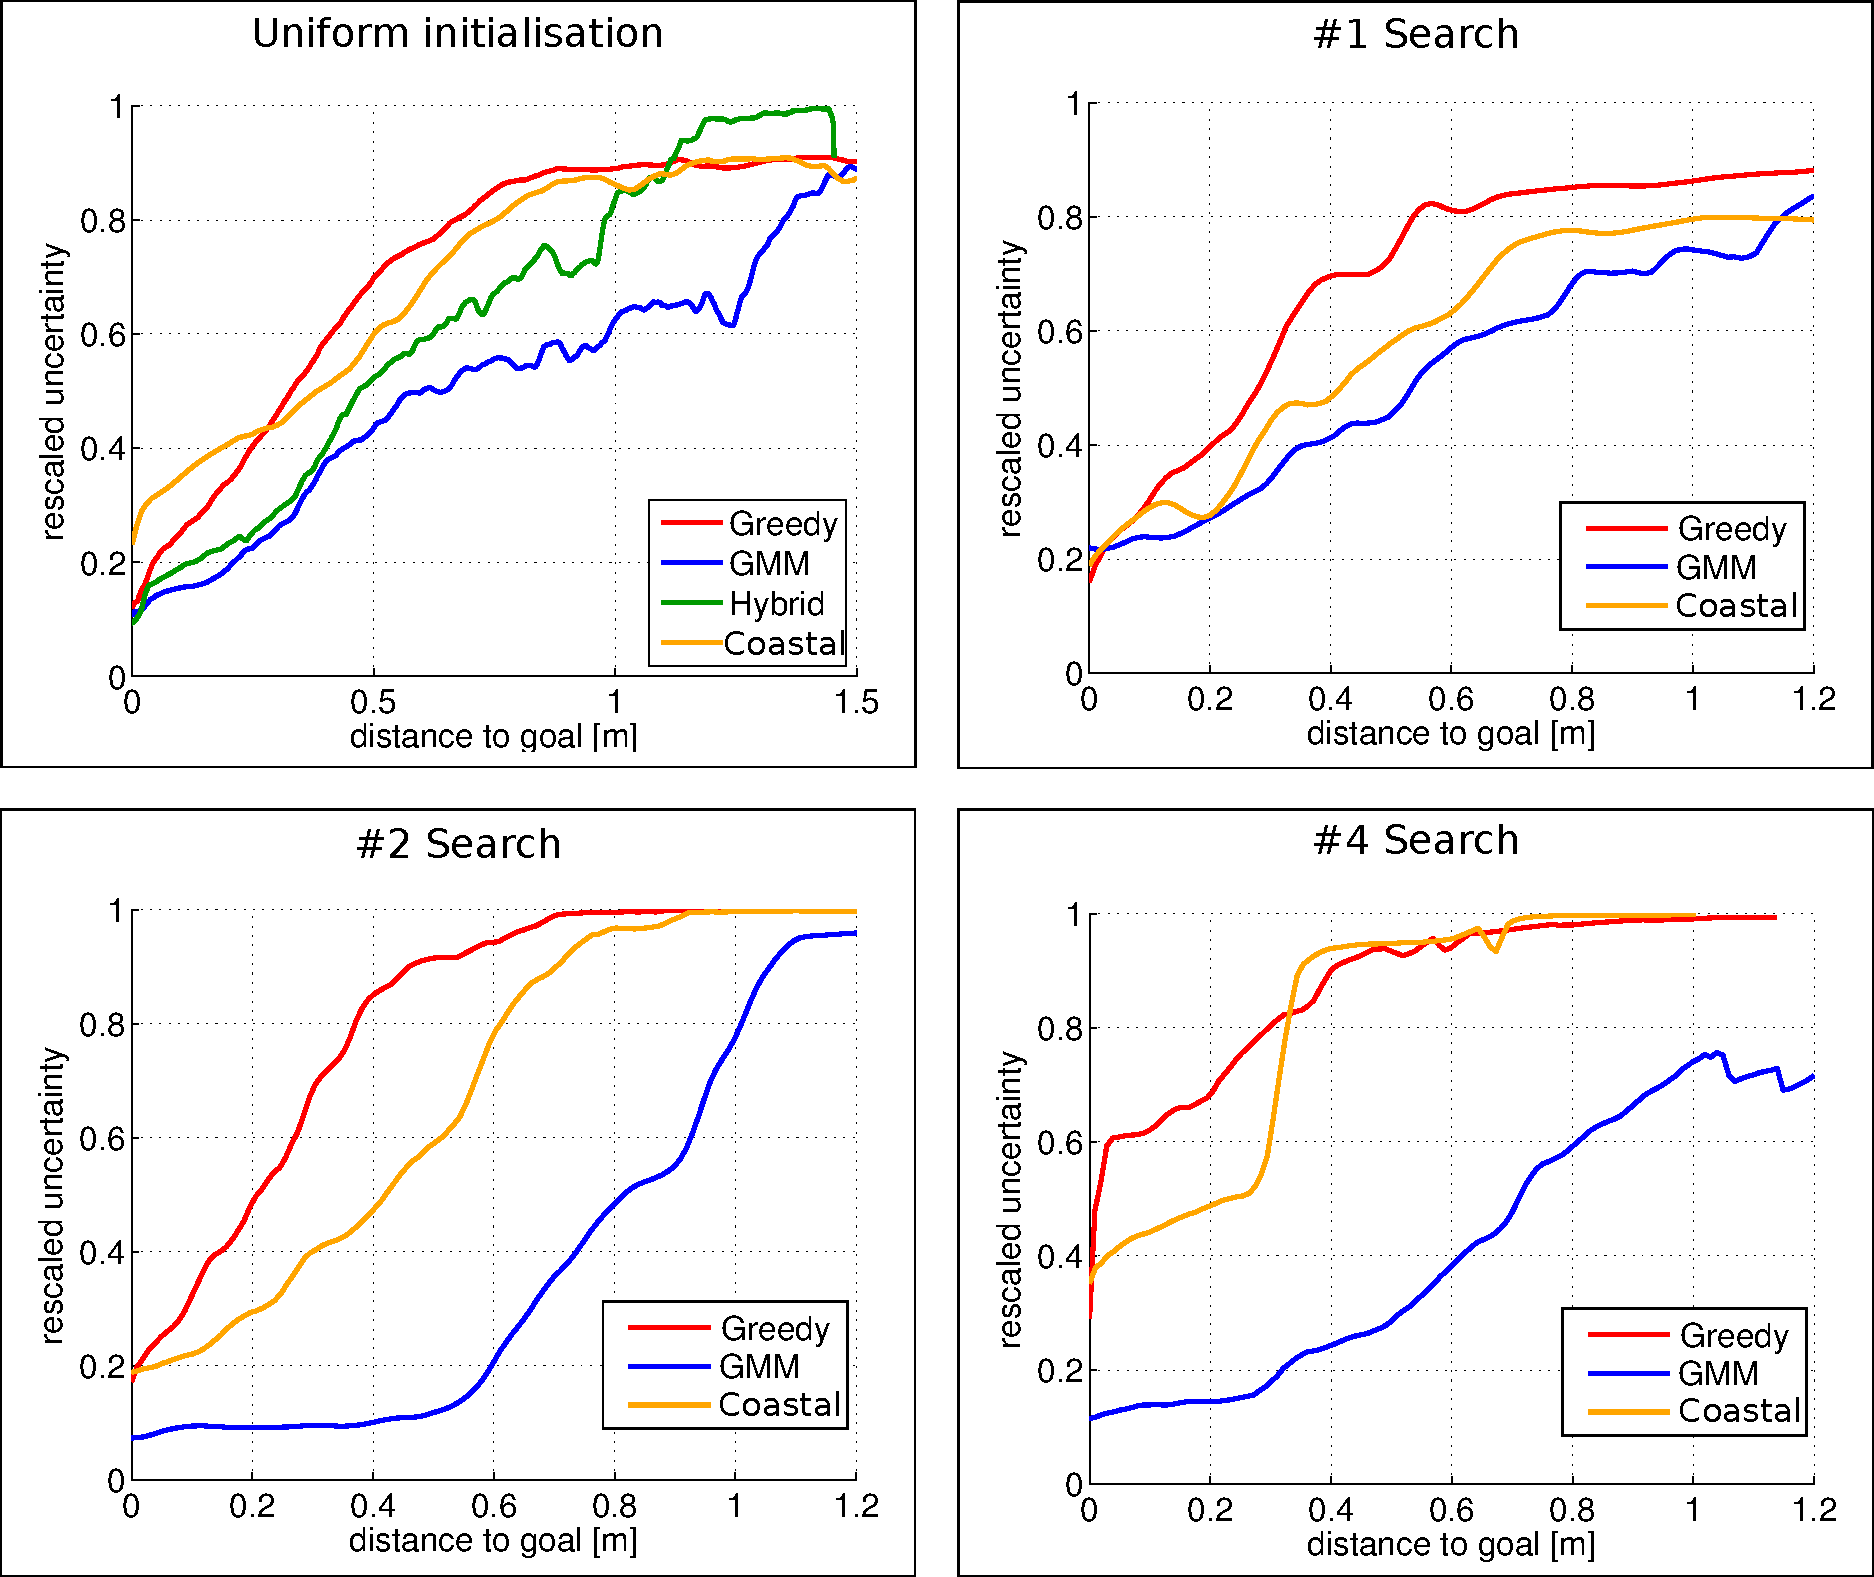
\includegraphics[width=0.95\textwidth]{./ch3-Search/Figures/Figure12}
\caption{Reduction of the uncertainty for the Uniform, \#1, \#2 and \#4 experiment, the expected value is reported
\textit{Top left}: Uniform initialisation, expected uncertainty for the Greedy (red), GMM (blue), Hybrid (green) \& Coastal (orange) search
 strategies.
\textit{Top right:} Experiment \#1. \textit{Bottom left:} Experiment \#2. \textit{Bottom right:} Experiment \#4.}
\label{fig:uncertainty}
\end{figure}


Figure \ref{fig:uncertainty} shows the normalised uncertainty with respect to the distance remaining to the goal for all experiments, 
(\#3 is excluded being similar to the \#2). 

The results show which methods actively minimise the uncertainty and which methods find the goal whilst being more dependent on chance. 
For all the reported experiments the GMM (learned from human searches) reaches a lower expected uncertainty than all other search algorithms. 
For the Uniform and \#1 search experiment, all methods reach the same final uncertainty level. However, for the \#2 and \#4 experiments, 
the GMM reaches the goal with significantly lower uncertainty. It is inferred that the GMM model actively minimises the uncertainty 
which is also reflected in the distance it takes reach the goal in comparison with the other methods.

While  the Greedy (\#2) and Coastal (\#4) are faster than the GMM method, Table \ref{tab:mean-var-distance}, both have a far higher level 
of uncertainty at the arrival which leads to the assumption that chance has a non-negligible effect on their success. 



%%%%%%%%%%%%%%%%%%%%%%%%%%%%%%%%%%%%%%%%%%%%%%%%%%%%%%%%%%%%%%%%%%%%%%%%%%%%%%%%%%%%%%%%%%%%%%%%%%%%%%%%%%%%%%%%%%%%%%%%%%%%%%%%%%%%%%%%%
%																	%
%				Conclusion 		 										%
%																	%
%%%%%%%%%%%%%%%%%%%%%%%%%%%%%%%%%%%%%%%%%%%%%%%%%%%%%%%%%%%%%%%%%%%%%%%%%%%%%%%%%%%%%%%%%%%%%%%%%%%%%%%%%%%%%%%%%%%%%%%%%%%%%%%%%%%%%%%%%

\FloatBarrier
\section{Conclusions}

In this work we have shown a novel approach in teaching a robot to act in a partially observable environment. 
Through having human volunteers demonstrate the task of finding an object on a table, we recorded both the 
inferred believed position of their hand and associated action (normalised velocity). A generative model
mapping the believed end-effector position to actions was learned, encapsulating this relationship. 
As speculated and observed, multiple strategies are present given a specific belief. This can be interpreted as the fact that 
humans act differently given the same situation. 

The behaviour recorded from the human demonstrations, encoded as set of expected sensations, showed
the presence of trajectories which both remained near to the edge and corner features but also 
trajectories which remained at a distance. Risk-prone and risk-averse behaviour was further 
confirmed by the overlap of the risk factor of Human and GMM generated trajectories with that of the Greedy
risk factor. According to the feature-based factor, more than 70\% of the human search trajectories were considered
to be risk-averse whilst 93\% according to the Risk factor. Similarly the GMM search trajectories showed to be
89-88\% risk-averse.

In terms of the comparative study, the GMM controller is more adapted to dealing with situations of high uncertainty and 
accounts for it better than Greedy or Coastal planning approaches. This is evident in the experiment
where the believed position and true position of the end-effector were significantly far apart and distant from salient areas. 
Future questions of scientific value to be addressed are to which extent do humans follow the reasoning 
of a Markov Decision Process in a partially observable situation where the state space is continuous 
(the problem has been partially addressed in \cite{Bake_Saxe_Tene_2011} for discrete states and actions). 

A drawback of the PbD-POMDP approach is that the quality of the learned policy is dependent on the abilities 
of the human teacher. If the teacher is good (on average) then the transferred policy will be adequate, if however
the human is suboptimal at performing the task, then the resulting policy will be poor. An autonomous way of
evaluating the quality of the demonstrations whilst learning a policy is necessary. In the next chapter, ``Chapter 4'', we 
demonstrate that by introducing a cost function and using a Reinforcement Learning approach we can account
for poor demonstrations and increase the quality of the policy.


%A further aspect of interestis to study the situation where multiple beliefs are present and investigate how humans 
%perform simultaneous localization and mapping as opposed to active localization which was the area of interest of 
%this research. 


% Basically talk about the drawback and introduce the next chapter.












  \fi
\ifdefined	\gDisplayPegSocket		\chapter{Peg in hole}

In Chapter 3, we demonstrated that we could learn a search policy and successfully transfer it to a robot apprentice
from demonstrations of human teachers for a task consisting of locating a wooden object on a table. 
In these search tasks our approach is based on the fact that intuition and knowledge exhibited by the human teachers, 
during the search, gives a good balance between exploration and exploitation actions which can then be encapsulated in 
a generative Gaussian Mixture Model (GMM) and be subsequently used as a control policy. 
The approach is satisfactory when extracting the many different behaviours demonstrated by the human teachers and reproducing 
them. However for learning an optimal or near optial policy with a unique behaviour the using  
of this approach will not necessarily result in a efficient policy. For the GMM we model
both the good and the bad search strategies exhibited by the human teachers. If the task is difficult and many possible solutions exist, such 
as in the previously discussed blindfolded search task in Chapter 3, many demonstrations will be required for search patters to
emerge and be encoded in the GMM. Otherwise the GMM needs to be combined with another policy as previously shown (Hybrid GMM-Greedy 
policy). 

%  This sentence is hard to follow. Break it into two sentences. What do you mean by goal-oriented? 
%  It is not clear which shortcoming you want to highlight. Is the requirement for consistency or for goal-orientedness? 
% Obviously, any task < no? The consistency requirement is also somewhat contradictory with the fact that you were embedding different 
% styles of search across demonstrations.

GMM does not discriminate between behaviours, as the Expectation-Maximisation (EM) algorithm used to 
learn the GMM policy ignores the quality of the demonstrated data. The EM algorithm does not contain a cost or 
reward function, encoding the objective of the task, which is common practice in Planning and Reinforcement Learning (RL). 
In the case of a difficult task where there are mostly bad demonstrations, the GMM search policy will reproduce suboptimal behaviour.
Additionally there may be that no good teachers, however by combining different components from 
individual demonstrations a good search strategy can be extracted.


%teachers are not good at the task individually and maybe only a few demonstrations are the best, whilst the majority are bad.
%There the task undertaken is implicitly encoded, as there is no cost function which is optimised, in 
%the GMM and as a result the taught behaviour has to be goal oriented and consistent, which is not always the case in a blindfolded search task. 

To overcome the above mentioned limitations, we introduce a binary cost function as a means of ranking the human teachers' demonstrations.
To this end, we combine our PbD-POMDP approach with an Actor-Critic Reinforcement Learning (RL) framework which 
is close to Fitted-Value Iteration(FVI) and other Experience replay methods. This new method we refer to as RL-PbD-POMDP. 
Our objective is to avoid the noisy explorative rollouts, a weakness common to all RL approaches, and only rely on 
the data provided by the human teachers. Autonomous exploration in RL can be seen to have three problem areas.

Firstly it is time consuming and is typically only applicable where an exhaustive exploration 
of the entire state or parameter space is feasible, such as in the inverted pendulum or mountain cart type problems. 
The universal exploration method, used throughout RL, is state independent (sometimes state dependent) white noise 
which results in an entire exploration of the state space. This
is neither practical nor feasible for the type of search problems we are considering. Secondly in this search 
problem as we are using a physical robotic system the exploration cannot be random as this would be dangerous.
Finally it is imperative that both the PbD-POMDP and RL-PbD-POMDP receive the same information. This would enable a fair comparison 
between the two algorithms and support our hypothesis that the RL-PbD-POMDP provides an improved policy 
with only human demonstrations as input.

%We chose a search and Peg-In-Hole (PiH) task
We analyse our RL-PbD-POMDP approach on a power-socket Peg-in-Hole (PiH) search task. In this task, human teachers must demonstrate 
to a robot apprentice how to search for and connect a plug to a power socket, see Figure \ref{fig:experiment_setup} (\textit{Left}). 
The first part of the task, the search for the socket, is similar to the table wooden-block setup in the previous chapter. 
However the connection of the plug to the power socket, the PiH component, requires a higher level of precision.
In Figure \ref{fig:experiment_setup} (\textit{Right}) the robot reproduces the behaviour demonstrated by the teacher.

% Show figure of the task setup.
\begin{figure}[h]
  \centering
  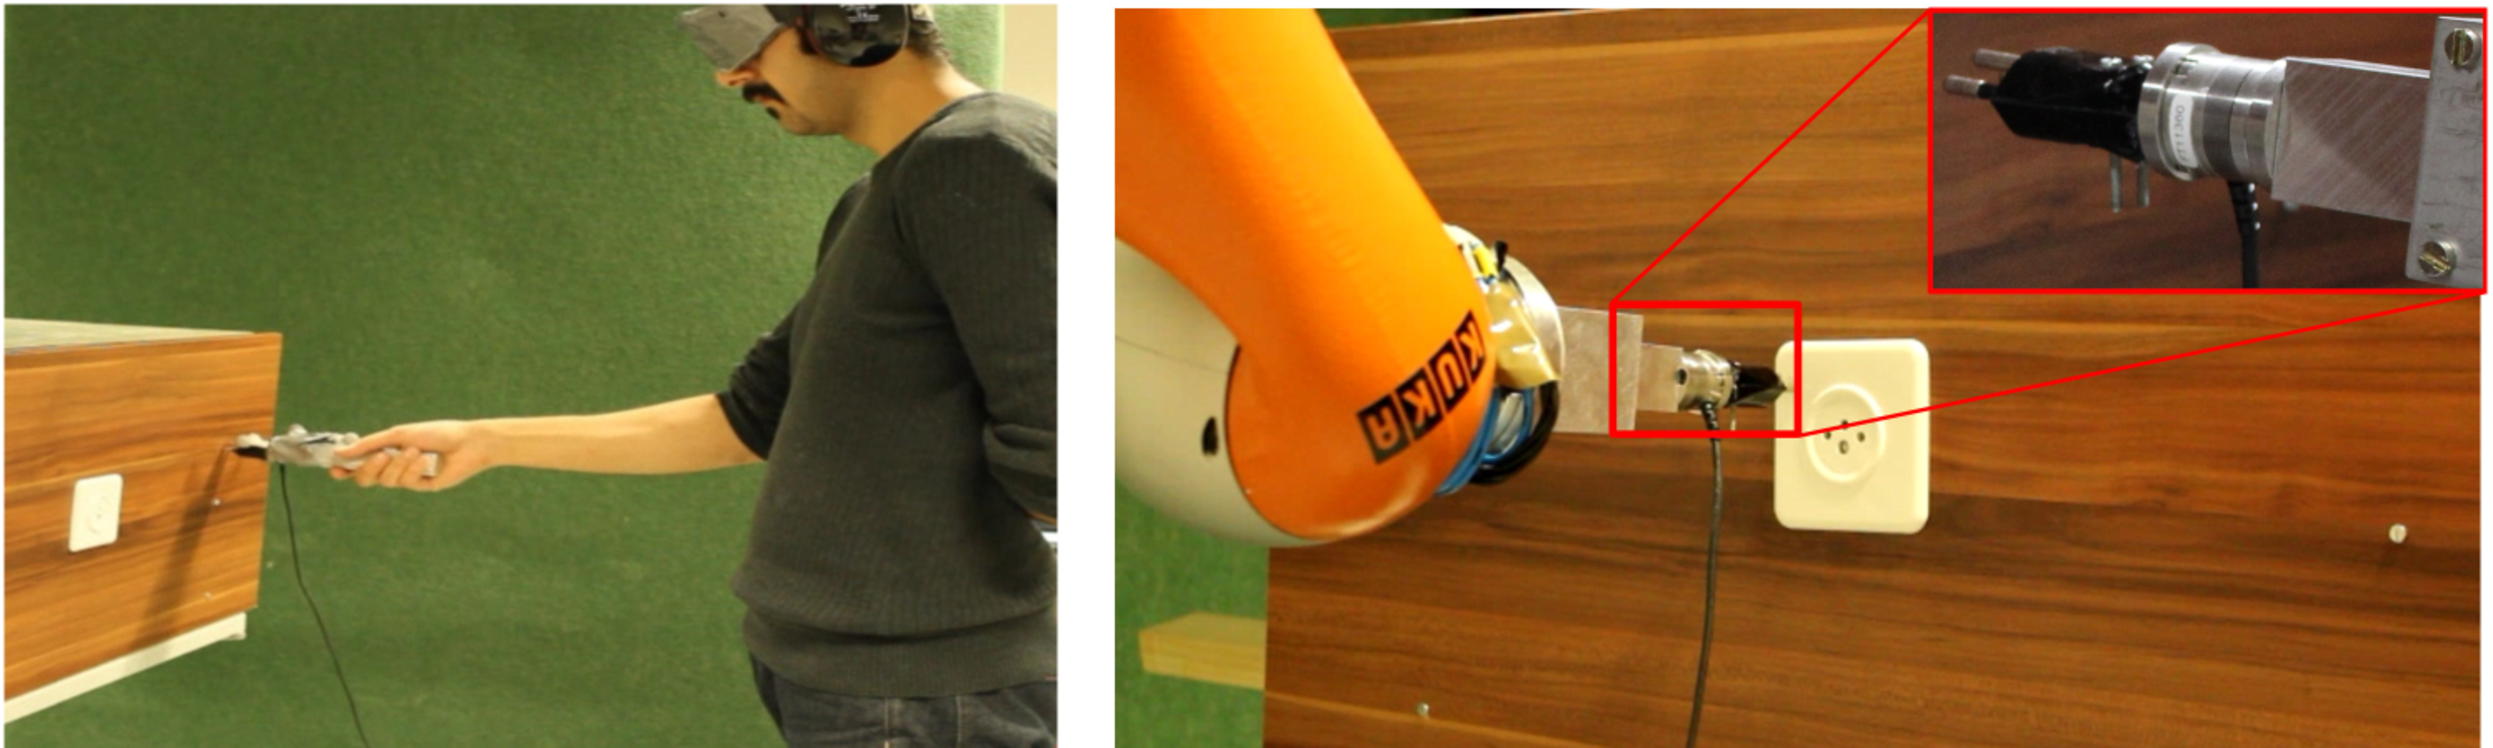
\includegraphics[width=0.95\textwidth]{./ch4-PiH/Figures/Fig/human_example_search.pdf}
  \caption{Peg-in-hole (PiH) search task. \textit{Left:} A teacher is wearing ear defenders (to impede any hearing) and 
  a blindfold. He first searches for the socket's location and then attempts to establish a connection. Force 
  and torque information is obtained from an ATI 6-axis force torque sensor at the end-effector of the tool held by the teacher.
  \textit{Right:} The KUKA LWR4 robot equipped with the same force torque sensor and plug reproducing the teacher's demonstrated behaviour.}
  \label{fig:experiment_setup}
\end{figure}


%(\textit{Top-right}), we illustrate the setup of the search task. The diagram shows
%the distribution of the initial starting position (in orange) of the human teachers. As was the case in our previous search experiment
%in Chapter 3, the teacher is disoriented before each trial but knowns that his initial heading will be the same, facing the wall. 
%The human teachers are deprived of visual information (they are blindfolded) and their hearing sense is significantly 
%reduced (by wearing ear defenders).  
%QIn the \textit{Bottom-left} quadrant we
%can see an example of a human teacher trying to accomplish the search and connection task, and to the \textit{Bottom-right} the KUKA
%LWR robot apprentice is reproducing a search policy learned from the teacher.

\section{Outline}
\begin{itemize}
  \item \hyperref[ch4:background]{\ref{ch4:background}   Background}\\
  We review aspects of the literature related to the Peg-in-hole problem and Actor-Critic Reinforcement Learning 
  with an emphasis on Fitted methods (also known as Batch or Experience replay), which we adapt to our GMM policy.
  \item \hyperref[ch4:experiment]{\ref{ch4:experiment}   Experiment methods}\\
  We detail the Peg-in-Hole search task, the number of participants (teachers) which provide demonstrations, the 
  type of data which is recorded and the representation of the human's location belief.
  \item \hyperref[ch4:learning-value-actor]{\ref{ch4:learning-value-actor} Learning Actor and Critic}\\
  We detail the representation of the Actor and the Critic and how they are learned in a Fitted Policy Evaluation 
  framework.
  \item \hyperref[ch4:control_architecture]{\ref{ch4:control_architecture} Control architecture}\\
  The learned behaviour is demonstrated on a 7 Degree of Freedom (DoF) articulated robot, named KUKA LWR4. 
  We detail the hybrid position-force controller and dynamical field modulation heuristic which is used in 
  combination with the learned behaviour policy from the human teachers.
  \item \hyperref[ch4:results]{\ref{ch4:results}  	 Results}\\
  We perform a set of 5 simulated experiments to test the generalisation, the importance of data provided by the human 
  teachers and the performance against simple search approaches to find the location of the socket. We further perform 
  3 experiments on the real robotic platform to test the generalisation of the learned policy on different power sockets.
  \item \hyperref[ch4:conclusion]{\ref{ch4:conclusion} Conclusion}\\
  The RL-PbD-POMDP policy achieves an important improvement over the previous PbD-POMDP approach
   by learning a value function over the belief space using approximate dynamic programming (part of FVI) and using it 
   to update the parameters of our GMM policy. We evaluate the ability of the policies to generalise to novel sockets 
   and different socket locations, both in simulation and on the KUKA LWR robot.
   The RL-PbD-POMDP approach consistently proves to be better. More importantly the RL-PbD-POMDP approach performs 
   significantly better when it is used on the worst teacher's demonstrations, which mitigates the \textbf{original assumption} that 
   teachers have to be consistently efficient at the task.
\end{itemize}

\section{Background}\label{ch4:background}

\subsection{Peg-in-hole}

The Peg-in-Hole (PiH) task is one of the most widespread step in industrial assembly and manipulations processes, with 
examples including the assembly of vehicular transmission components \cite{search_strategies_icra_2001} and 
valves \cite{online_gpr_icra_2014}. To be successful, the estimated
position of the robot's end-effector and workpiece must be precise. Typically, the clearance between peg and plug 
is very small leaving little room for error. As a result, variations in the assembly's components 
in combination with position uncertainty can result in either jamming during the insertion process or in failure for 
the plug finding the hole. This created a need for adaptive search and insertion policies for PiH, which has been driving research 
in this area. 

From the literature, we identified the different components in PiH solutions. 

All approaches use to some extent a vision system to estimate the position of the workpiece. 
For instance in \cite{peg_personal_icra_2010} a PR2 is equipped with a checkerboard to facilitate pose 
estimation  of the plug with respect to a power outlet whose position is extracted through a vision 
processing pipeline. An initial connection is attempted by visual servoing which is successful 10\% of the 
time. Given an estimate of the workpiece's position, a common approach is to follow either a blind increasing spiral 
Cartesian trajectory or parametrised policies which guarantee that all positions on the workpiece have been visited.
In \cite{peg_personal_icra_2010}, if the PR2 initially fails to connect the plug to the socket
a spiralling outward motion is carried out with 2mm increments which obtains an overall 
success rate of 95\%. For this approach to be applicable to a generic robot, it would require the addition of an
external camera and checkerboard to the robot in question which might be cumbersome. In our work we consider a 
vision free system.

%To increase the chances of a connection these approaches use a compliant controller 
%which usually includes a hybrid force/position controller.
%In \cite{peg_personal_icra_2010} a PR2 executes a parameterised policy designed to connect a plug to a power outlet
%in order for the PR2 to recharge itself. The plug is equipped with a checkerboard to facilitate pose estimation
%of the plug with respect to power outlet whose position is extracted through a vision processing pipeline.
%An initial connection is attempted by visual servoing which is successful 10\% of the time. 
%When unsuccessful a spiralling outward motion is carried out with 2mm increments. 
%This method achieved an overall success rate of 95\%.
%The hybrid control paradigm \cite{hybrid_1992} was used throughout the execution of the task.
%The first approach does not consider reproducing the F/T profile 
%but rather follows a position trajectory whilst being compliant.


Another approach (which has been confined to academic circles) follows the data driven 
Programming by Demonstration (PbD) framework. Teleoperated or kinesthetic demonstrations by a human teacher 
are recorded and a policy is learned and fine-tuned so as to reproduce the same (F)orce/(T)orque profile as 
that demonstrated by the human teacher. 

% PbD: reproduce the F/T profile irrespective of the learned position trajectory DMP
In \cite{fast_peg_pbd_icmc_2014} the authors learn a PiH policy for the Cranfield benchmark object.
A vision system obtains the pose parameters of the object whilst a human teacher  
demonstrates trajectories, through teleoperation, in the frame of reference of the object. 
A time-dependent policy represented with Dynamic Movement Primitives (DMP) \cite{Schaal04learningmovement} 
encodes the recorded Cartesian end-effector pose. In \cite{trans_workpiece_icra_2013}, a F/T profile 
is encoded separately by a regressor parameterised by radial basis functions. Successive refinements of the DMP policy are achieved through 
using force feedback to adapt the parameters of an admittance controller. This results in the policy having
similar force profiles to the human teachers. Further applications based on this method have been 
performed \cite{sol_pdg_pbd_2014} with the incorporation of a disturbance rejection policy. Reproducing exactly 
the same force torque profile for the full trajectory which is encoded in a time dependent dynamical system might be unnecessary as the force torque profile is 
predominantly useful during the final stage of the PiH task, where the insertion can cause jamming. 
The force torque information can be used to rectify this problem \cite[Chap. 5]{Kronander2015}. A 
hybrid control paradigm \cite{hybrid_1992} can also be used to control the sensed force feedback with the environment.
We make use of the hybrid control paradigm in this work in combination with a time-independent dynamical system.

Reinforcement learning has also been used in combination with DMP to learn PiH policies. In \cite{learn_force_c_icirs_2011}
an DMP policy is initialised with kinesthetic demonstrations of opening a door and picking up a pen. The recorded Cartesian 
trajectories are encoded in a parameterised DMP policy and augmented with a F/T regressor profile. A reward function is designed, 
encoding desirable properties of the F/T profile such as smoothness and continuity. After 110 trials the policy
was found to be a 100\% successful. In \cite{learn_admittance_icra_1994} a 18 dimensional input (sensed position, previous position and force) 
and a 6 dimensional output (linear and angular velocity) neural network is learned by associative reinforcement learning. 
During the learning process the plug is randomly positioned within the vicinity of the hole. After a 100 executions and 
updates, the policy was shown to be successful and was able to generalise across different geometries and clearances.
Our work is similar in its approach, however we will not be considering autonomous rollouts common 
in RL, but will rely solely on the initial data provided by human teachers.

All the above policies were learned from human demonstrations and encoded by a regressor function and
optimised to reproduce a desired F/T profile. Other approaches to the PiH problem 
are predominantly based on heuristic search mechanisms and compliant controllers.

% Blind search stragegies
In \cite{search_strategies_icra_2001} different blind search policies are analysed for the insertion of a spline toothed hub 
into a forward clutch. The state space is discretised into points so that the distance between two 
neighbours is smaller than the clearance of the hole, which is known as a spray point coverage. Different search 
strategies are evaluated which ensure that all the points are visited. It is found that paths following  
concentric circles gradually spiralling inwards are the most effective method for finding the hole. This concentric circle
search strategy has been applied in many PiH tasks. For instance in \cite{peg_imcssd_2015}, a PiH heuristic 
policy was developed to connect a 5-pin waterproof industrial charger to an electric socket. The authors 
estimated the pose of the socket through a vision system and used a force controller in combination with a 
blind spiral search policy to achieve a connection and demonstrated their approach to be reliable. 
These blind search strategies do not consider actual state uncertainty and only work well when the plug or 
peg is within the vicinity of the socket. In our work we consider no visual information which leads to 
high state uncertainty making the direct application of such blind search methods ill-suited.

% Do it the same way that humans do it: Does not use FT sensor
In \cite{intuitive_peg_isr_2013} the authors observe that humans lack the precision and sensing 
accuracy of robotic systems, but nevertheless, are more proficient than robots at PiH. The authors state that when 
humans try to connect a square plug to a socket, they rub the plug against the socket's 
outlet without looking. It is thought that the inherent compliance in humans' motor control  
is the key to our success at PiH tasks \cite{compliant_manip_icra_2008}. 
The authors introduce an Intuitive Assembly Strategy (IAS) inspired by the above observation which 
does not require the hole to be precisely localised. The IAS search strategy is based on compliant 
spiral motion and the execution of the search trajectory is performed with a hybrid force/position controller.
We also have observed that humans are good at accomplishing such tasks and we exploit this in our own PiH policy. 
We further consider different types of geometric objects whilst only considering haptic information.

The spiral strategy is widely used in industrial applications due to its simplicity, 
however, it is a blind search method. Another approach when dealing with the assembly
process consists of fine-tuning parameters of predefined policies. In \cite{online_gpr_icra_2014}
the authors develop an online Gaussian Process policy optimisation of an assembly task. They 
demonstrate that by learning the dynamical model of the task during execution, it is faster than offline methods, 
such as Design of Experiment (DOE) or Genetic Algorithms.

%  Aude comment
% All this survey of state of the art refers primarily to the task at hand (peg and hole task), but do not refer to 
% the particular RL-Pomdp approach. This is ok, since you review the latter in Chapter 2 , but explain this to the 
% reader before starting bck, by stating that here you will review only work done on solving this particular 
% task and refer to reader back to specific sections in chapter 2 for review of state of the art on the other 
% relevant topics (list them).

\subsection{Actor-Critic \& Fitted Reinforcement Learning}

In our PiH-search task, to learn a POMDP policy, we consider RL approaches which naturally handle continuous 
belief-state and action spaces, such as policy search/gradient methods. Chapter 2 gives an overview of 
such policy search methods. However, policy gradient methods are time consuming when the number of parameters 
is large compared with the state space, \cite{ACML_variance_2015}.
This results from the large variance of the policies' gradient, making the stochastic gradient ascent learning slow. 
In Chapter 3, the learned PbD-POMDP policy has over 80 Gaussian functions, each of dimension 7, and we expect the 
number of parameters of this RL policy to be of the same order. So instead we opt for an Actor-critic (AC) approach 
which has been reported and proven \cite{rl_ac_surv_2012} and with this approach the variance of the gradient update in 
AC methods has a smaller variance compared with actor methods (policy gradient). This results in a faster learning of 
the policy. 

Actor-critic \cite[Chap. 6.6]{sutton98a} is an RL approach in which the policy (actor) and critic (value function) 
have separate parameterization and can be represented by different functions, for instance the value function could be a 
decision tree and the policy a neural network. The advantage of an AC is that the policy can be chosen such 
that it is computationally efficient in evaluating actions and the value function does not necessarily have to have
the same input space as the policy.  %The parameters of both the actor 
%and critic are learned via gradient ascent on the Temporal Different (TD) error. 

The policy gradient theorem \cite{Sutton00policygradient} states that if the regressor functions of both the
actor and critic share the same basis functions (also called \textit{compatible} features) and their parameters are linear, 
then an unbiased estimate of the policies' gradient can be obtained. The drawback of this 
approach is that both the value function and policy have to be defined over the state-action space.  
This is restrictive and in addition it has been shown that Function Approximators (FA), such as linear models 
or neural networks, when combined with temporal difference learning, can diverge \cite{Safe_val_function_1995}.

As we are working in belief-space we seek a framework in which both the actor and critic can have 
their own parameterisation whilst guaranteeing convergence of the value function. All value function approximators, 
such as tile coding,  state aggregation, k-nearest-neighbour, locally weighted averaging and grid discretisation 
are all averagers and are guaranteed to converge in model based RL \cite{stable_FA_gordon_1995} when used with 
temporal difference learning. The key idea presented in \cite{stable_FA_gordon_1995} and which lead to the increase in popularity
of batch and fitted methods, is to separate the Bellman and value function in a synchronous update, that 
is, to first compute the Bellman update for all the sample states and then fit a value function via standard supervised 
learning techniques. The extension to a model-free approach with a kernel function approximator (locally weighted averaging, the 
kernel is a Gaussian function) known as Kernel-Based Approximate Dynamic Programming (KBDP) \cite{kernel_rl_ormoneit_2002}
has proven to be globally optimal in a continuous-space framework. This leads to the wider application of Batch RL methods 
such as Fitted Value Iteration (FVI) \cite{fvi_uav_2010} and Fitted Q-Iteration (FQI) \cite{EGW05} (Q-approximator is a random forest ensemble),
\cite{fqi_nips_peter_2009} to the RL community. By remembering all the state transition pairs and by applying multiple 
synchronous Dynamic Programming (DP) and function approximation updates, the problem of diverging value function approximators is resolved. 

Retaining all the data makes it in practice easy to apply function approximators which are not averagers, such as neural networks,
to RL problems. A successful example was Neural Fitted Q-Iteration (NFQI) \cite{Riedmiller2005} which 
uses a multi-layer perceptron to represent the Q-function for the cart-pole and mountain car problems and 
shows rapid convergence to optimal policies. It has since been used in many extensions, \cite{NAC_2008}, \cite{rl_gmm_2010}.
This has lead to the application of more sophisticated regression methods such the increasingly popular Deep Learning methods 
which are known as Deep Fitted Q-iteration (DFQ) \cite{Lange_riedmiller_2010} (used to learn visual control policies) 
and with recent work including learning to play ATRI and ping-pong games \cite{mnih-dqn-2015}, \cite{DRQ_AAAI_2015} (reviewed
in Chapter 2).

The reader is referred to \cite{approx_rl_overview_2011} for a literature review which includes a taxonomy of 
Batch RL methods and to \cite[Chap 2]{RL_state_art_2012} for a concise description Batch RL beginning at 
its origins, how it became popular with Fitted RL approaches and its continuation into Deep Learning.

The RL-PbD-POMDP framework which we will use in this chapter is also based on a Fitted approach, however we 
avoid performing the expensive maximisation over the continuous actions space, as in the FVI and FQI approaches, 
by fitted policy evaluation followed by policy improvement. We use a Gaussian Mixture Model to parameterise 
the policy and a Locally Weighted Regression (LWR) as the value function approximator.

% Entitle this Human Pilot Study and tell us in introduction that you first conduct a pilot study, 
%  analyse the result and use these to gear the design of the algorithm, etc.

\section{Experiment methods}\label{ch4:experiment}

% Entitle this Human Pilot Study and tell us in introduction that you first conduct a pilot study, analyse the result and use these 
% to gear the design of the algorithm, etc.

% You had only make participants? Explain to us the procedure. How many participants, how many trials, protocol, etc. 
% Have little titles for each section: Participants: number, gender, age. Methods: Recording systems (you already mentioned this in intro, 
% but perhaps move some of this here and give us a notion of framerate, precision of sensing, duration of experiment. Take one of our recent 
% articles on human studies (e.g. the two papers Mahdi just got out) for inspiration on how to document user studies.

%\subsection{Experiment setup}
%
%	environment, opti-track, ATI and precision of each of these
%
%% Recording System [Optitrack] fame rate, precision of sensing [error in position estimage, sensitivity of the force-torque profile]
% Duration of the experiment
%

%
% The human teachers are deprived of visual information (they are blindfolded) and their hearing sense 
% is significantly reduced (by wearing ear defenders).  
%

%We make the assumption that the human's believed location can be presented by a probability density function, which is assumed to be known. All subsequent 
%distributions can be obtained through the application of a Bayesian filter given that both the sensing and motion 
%information are provided by the force torque and motion capture sensors.

% The teachers are told and shown before hand the setup and 
% it is made clear to them that they will always be starting in the orange area facing the wall which we demarcated with tap. 

Figure \ref{fig:search_task_setup} (\textit{Top-left}), illustrates the PiH-search experiment setup. The orange area represents 
the teachers starting area and is assumed prior knowledge. The sockets are always positioned at the center of a fake wall (wooden plank) which is clamped to a table, see 
Figure \ref{fig:search_task_setup} (\textit{Top-right}) for an illustration. 

We consider one type of plug, Type J\footnote{http://www.iec.ch/worldplugs/typeJ.htm}, and three different power sockets. 
Power \textit{socket A}, has a ring around its holes, \textit{socket B} has a funnel, which we hypothesize should make 
it easier to connect, and \textit{socket C} has a flat elevated surface. See Figure \ref{fig:search_task_setup}
(\textit{Bottom}) for an illustration. 

\begin{figure}
 \centering
 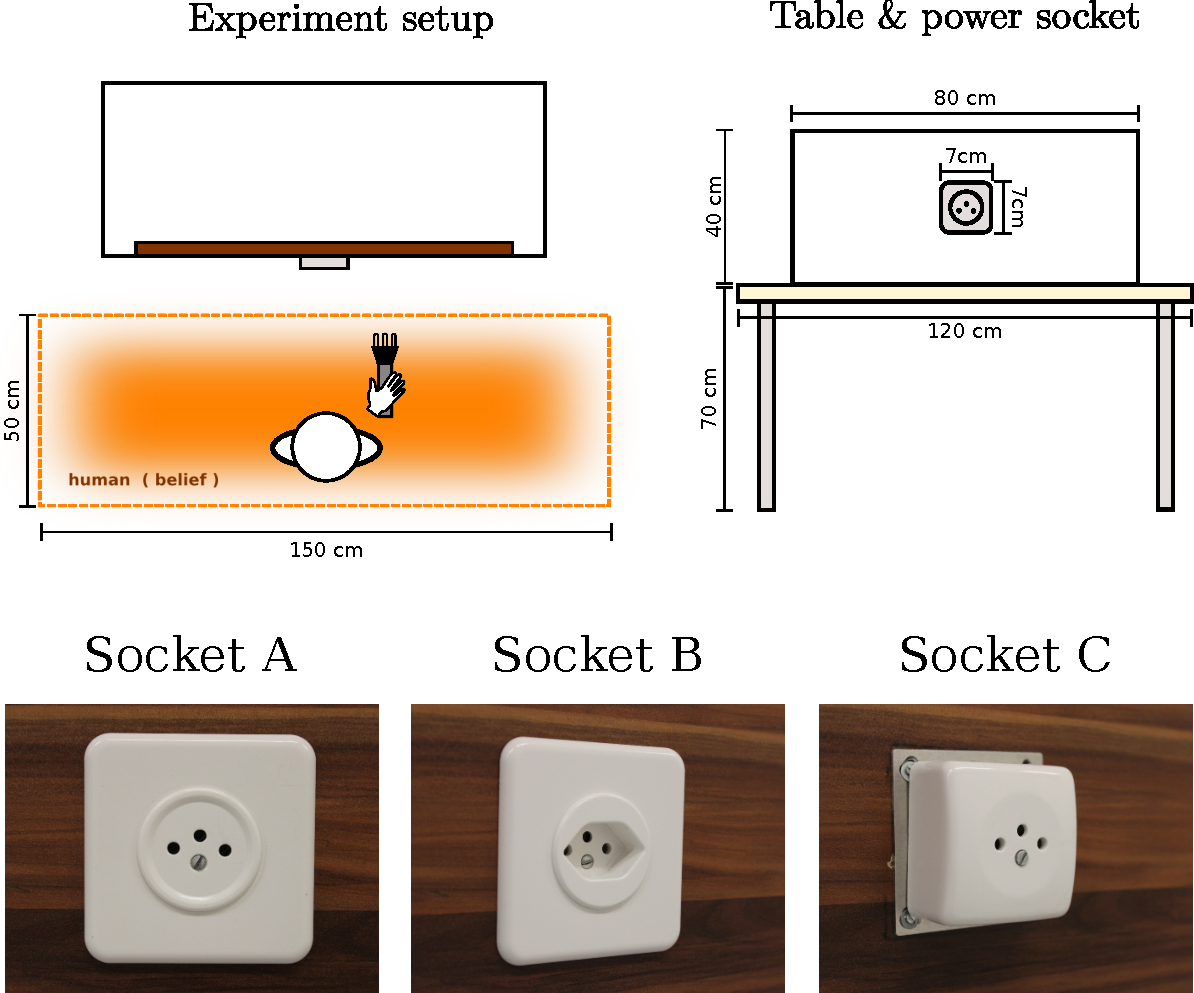
\includegraphics[width=0.8\textwidth]{./ch4-PiH/Figures/Fig/experiment_setup_and_design.pdf}
 \caption{The experimental setup. \textit{Top-left:} A participant (human teacher) is blindfolded and 
    placed within the orange rectangular area always facing the wall. \textit{Top-right:} Dimensions of the 
    the wall and socket. \textit{Bottom:} Three different power sockets, only socket A and B are used for data collection, socket
    C is purely used for evaluating the generalisation of the learned policy.}
    \label{fig:search_task_setup}
\end{figure}

The human teacher holds the plug which is attached to a cylindrical handle with 
an ATI 6 axis force torque sensor (Nano25 \footnote{http://www.ati-ia.com/products/ft/sensors.aspx}) 
to provide \textbf{raw} wrench $\phi \in \mathbb{R}^6$ measurements. We define the \textbf{actual} measurement 
to be a function of the raw wrench, $\tilde{y}_t = h(\phi_t)$, which is a binary feature vector. The feature vector encodes whether a contact is present 
and the direction in which it occurs, which is discretized to the four cardinalities.

On top of the cylinder there is a set of markers used by a motion capture system OptiTrack\footnote{http://www.optitrack.com/}
(which has millimeter tracking accuracy), 
see Figure \ref{fig:plug_cylinder}, to measure both linear, $\dot{x} \in \mathbb{R}^3$, and angular 
velocity, $\omega \in \mathbb{R}^3$, at each time step which is recorded at a rate of 100 Hz. The force and torque information 
from the ATI sensor is recorded at the same rate. 

\begin{figure}
 \centering
 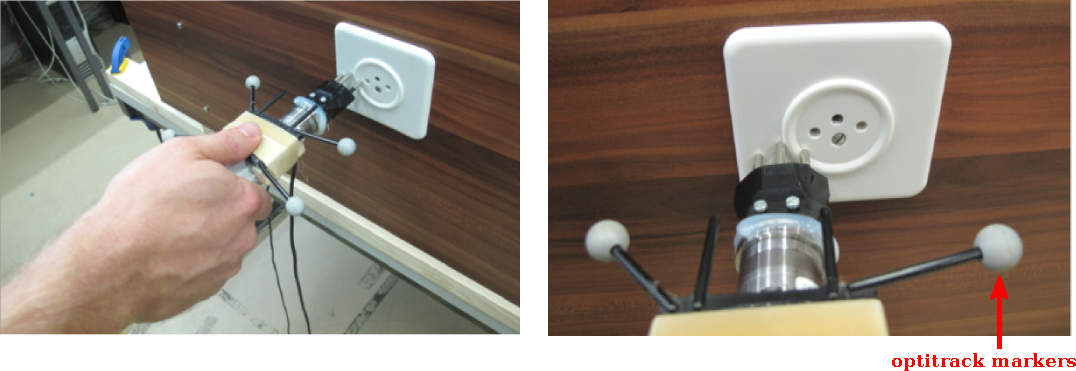
\includegraphics[width=0.8\textwidth]{./ch4-PiH/Figures/Fig/plug_socket_closeup.pdf}
 \caption{Human holding the cylinder plug holder, which is equipped with OptiTrack markers.}
 \label{fig:plug_cylinder}
\end{figure}

In this task, the human's location belief is represented by a probability distribution function. 
The participants' (teachers) initial belief is assumed to be uniformly distributed as depicted 
in orange area of Figure \ref{fig:search_task_setup} and that all subsequent beliefs can be inferred from the measured velocity 
and measurements provided by the ATI and OptiTrack sensors. The following section describes how the belief can be represented, 
computed and compressed.

\subsubsection{Belief state}
%\subsubsection{Belief probability density function}
% Before explaining the measurement model we detail what measurement $\tilde{y}_t$ is.
%This step essentially consists of applying a convolution kernel to the PMF where the covariance 
%is proportional to the measured velocity.
For the task at hand, the belief probability density function,  $p(x_t|y_{0:t},\dot{x}_{0:t})$,  
is a Point Mass Filter (PMF) \cite[p.87]{Bergman99recursivebayesian}, which is a  Bayesian filter.
It is parametrised by a set of grid cells containing valid probabilities 
and is recursively updated by the application of a \textbf{motion}, $p(x_t|x_{t-1},\dot{x}_t)$ 
and \textbf{measurement}, $p(y_t|x_t)$ model. The motion model updates the position of the probability density function 
and subsequently increases the uncertainty of the position.  The measurement model indicates areas 
of the state space from which a measurement $\tilde{y}_t$ could have originated. 
In Figure \ref{fig:PMF} (\textit{Bottom-right}) we illustrate the likelihood when an edge is sensed.

A PMF is chosen to represent the believed location of the plug as the sensing 
the sensing likelihoods are non-gaussian and lead to multi-modal distributions.  
A PMF is able to capture such non-gaussianity whilst remaining fully deterministic 
(which is not the case for a particle filter).

\begin{figure*}
 \centering
   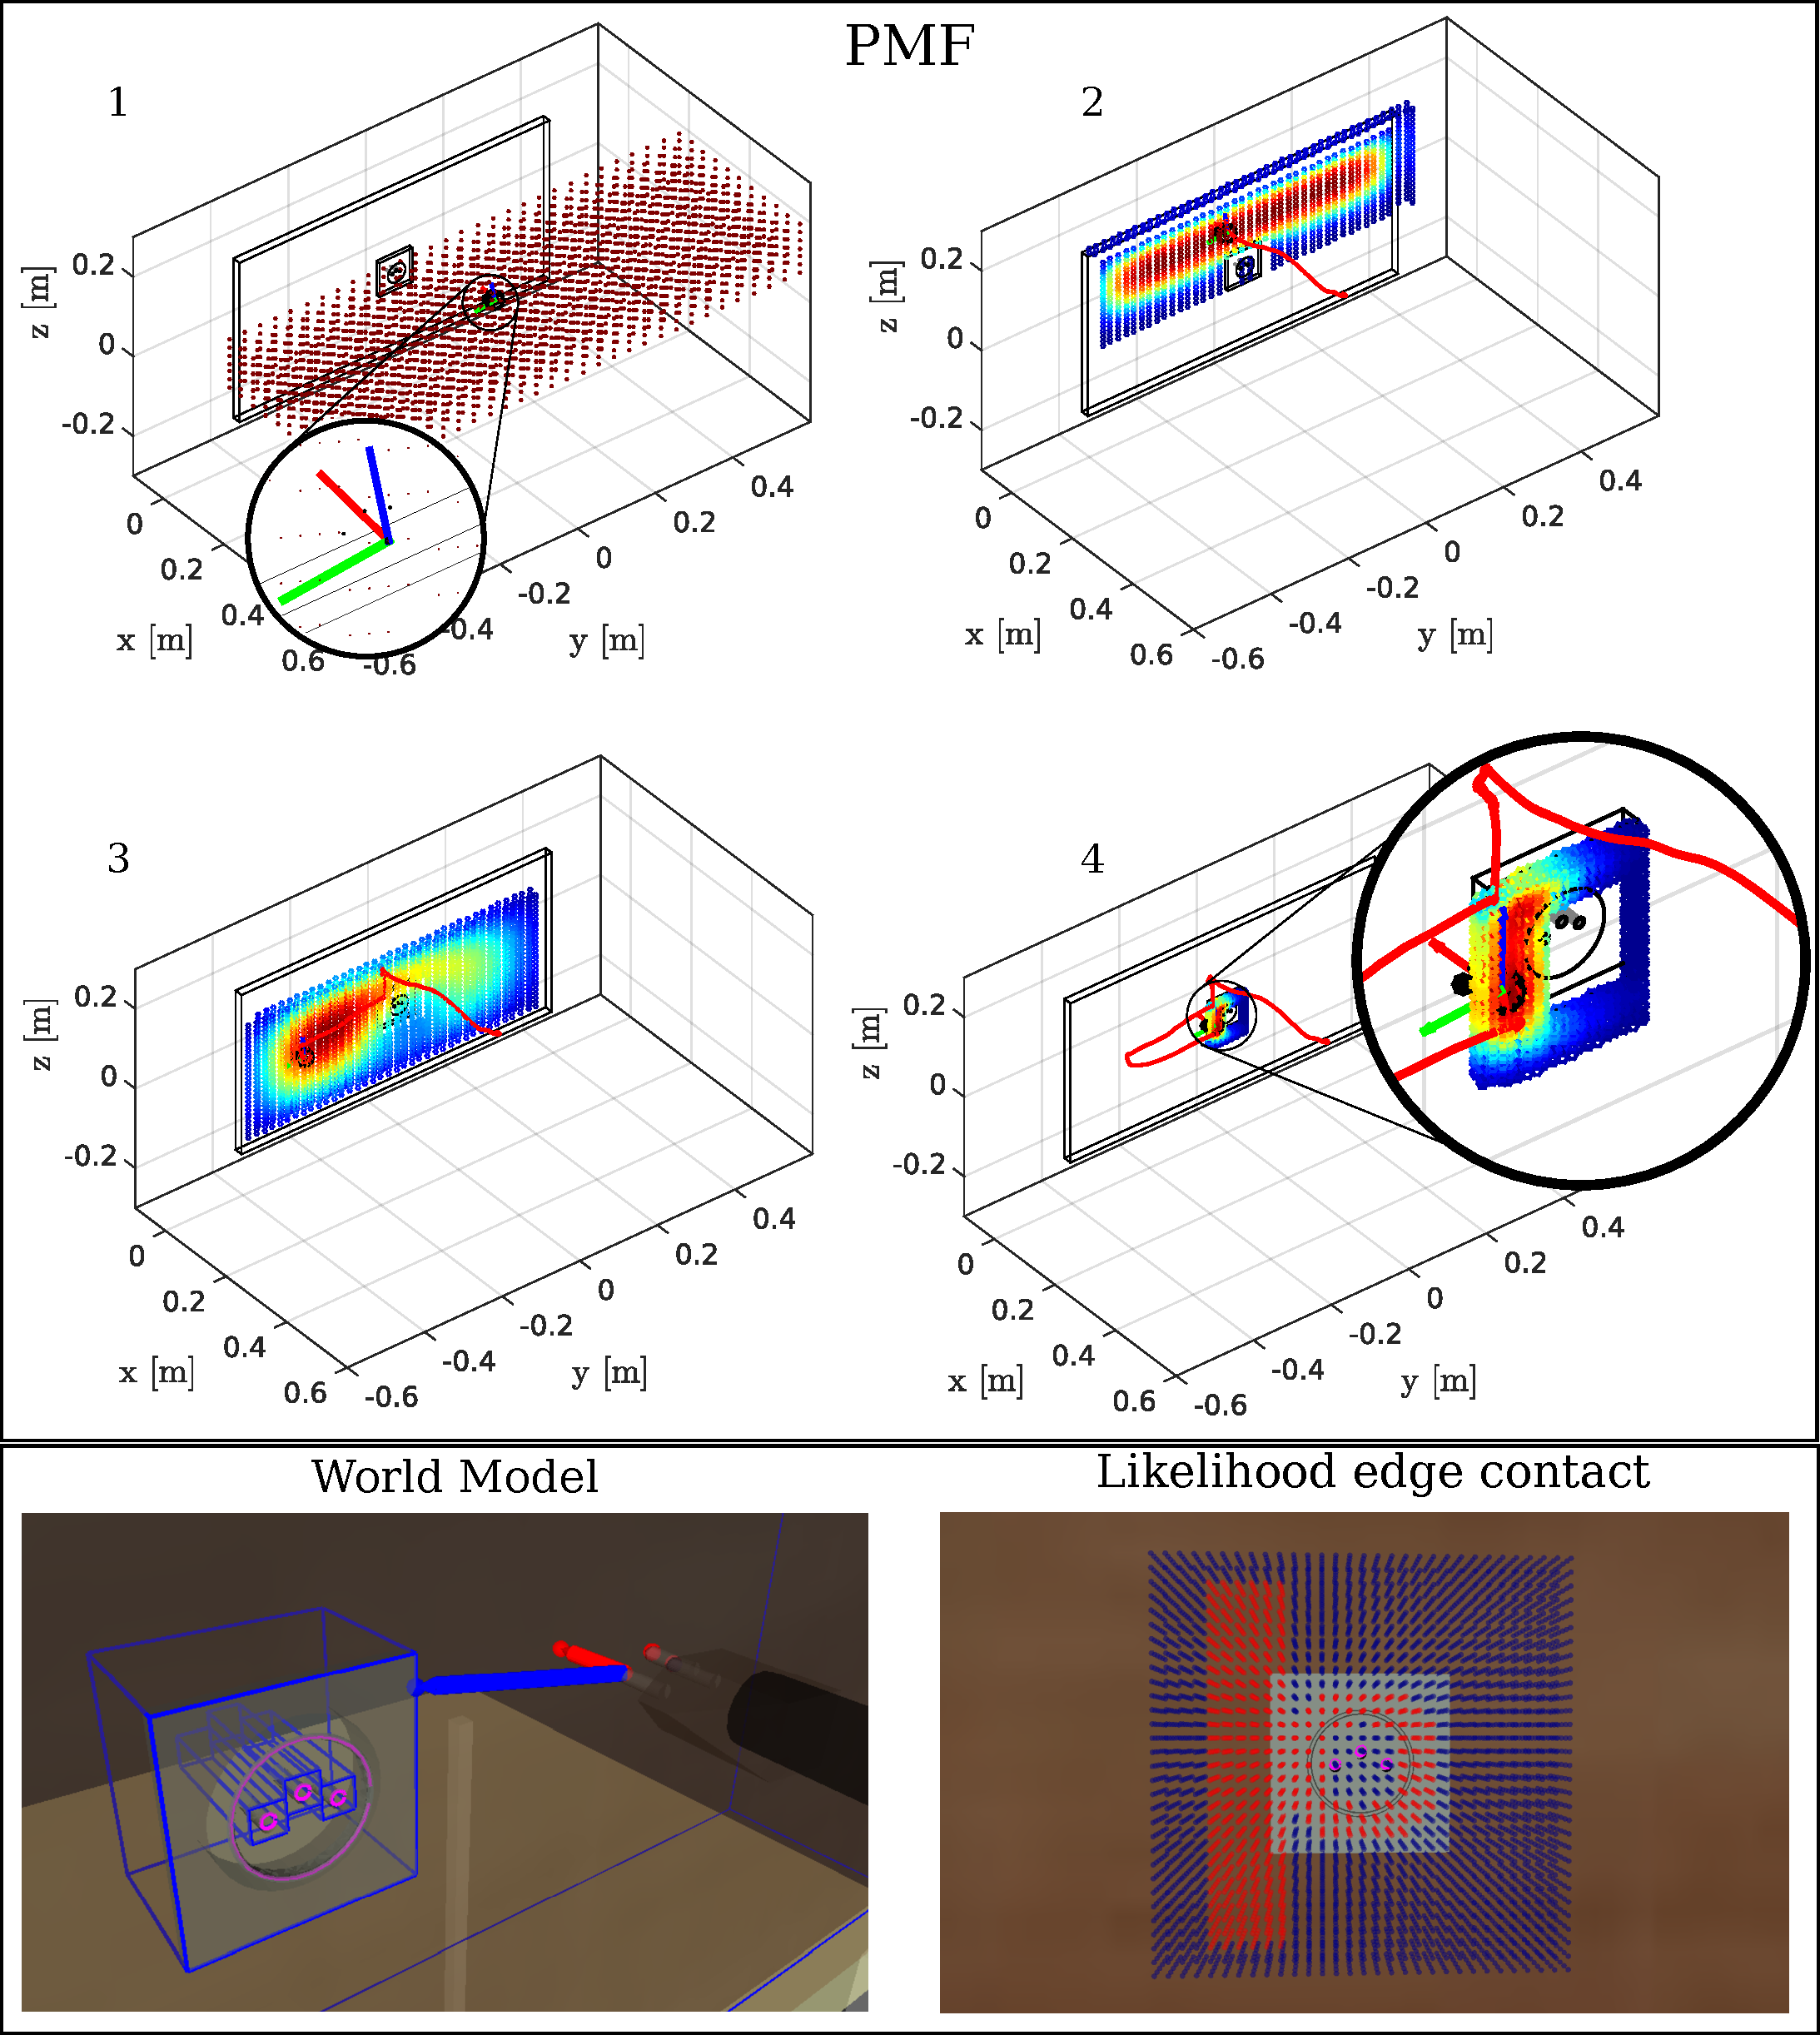
\includegraphics[width=\textwidth]{./ch4-PiH/Figures/PMF/pmf_likelihood_v2.pdf}
   \caption{\textit{Left:} Point Mass Filter (PMF) update of a particular human demonstration. (1) Initial uniform distribution spread over the starting 
   region. Each grid cell represents a hypothetical position of the plug. The orientation is assumed to be known. (2) First contact, the distribution 
   is spread across the surface of the wall. The red trace is the trajectory history. (3) motion noise increases the uncertainty. (4) The plug is in contact with a socket edge.
   \textit{Right}: \textbf{World model}: The plug is modelled by its three plug tips and the wall and sockets are fitted with bounding boxes.
   \textbf{Likelihood}: The plug enters in contact with the left edge of the socket. As a result, the value of the likelihood in all the regions, $x_t$, close the left edge take 
   a value of one (red points)  whilst the others have a value zero (blue points) and areas around the socket's central 
   ring have a value of one. }
  \label{fig:PMF}
\end{figure*}

The probability density function $p(x_t|y_{0:t},\dot{x}_{0:t})$ is high dimensional and thus it is 
impractical to directly learn a statistical policy $\pi_{\theta} : p(x_t|y_{0:t},\dot{x}_{0:t}) \rightarrow \dot{x}_t$
without some form of compression. One possibility would be E-PCA \cite{NIPS2002_2319} which extracts a set of 
representative basis functions which are aslo probability distributions. Although elegant this method 
requires a discretisation of the belief space which is computationally expensive. Instead we choose to 
compress the pdf to a belief space vector composed of the maximum a posteriori, $\hat{x}^{\mathrm{MAP}}_t = \argmax_{x_t} p(x_t|y_{0:t},\dot{x}_{0:t}) \in \mathbb{R}^3$, and the differentiation entropy, 
$U = H\{p(x_t|y_{0:t},\dot{x}_{0:t})\} \in \mathbb{R}$. All pdfs in our recorded data set $D$ are transformed to 
a belief space feature vector, $b_t = [\hat{x}^{\mathrm{MAP}}_t,U]^{\mathrm{T}}$. 

Each participant's demonstration results in a dataset $D=\{\dot{x}^{[i]}_{1:T},\omega^{[i]}_{1:T},\phi^{[i]}_{1:T},b^{[i]}_{1:T}\}$, 
where the upper index $[i]$ references the ith search trajectory (also one execution of the task or one episode) and 
subscript $1:T$ denotes the time steps during the trajectory from initialisation $t=1$ until the end $t=T$. 
%The data consisted of the plug's linear velocity, $\dot{x} \in \mathbb{R}^3$, 
%angular velocity $\omega \in \mathbb{R}^3$, the sensed wrench $\phi \in \mathbb{R}^6$ (force-torque),
%and the belief state, $b$, over the plug's location.

\subsection{Participants and experiment protocol}

To perform the PiH search tasks we recruited 10 student volunteers to be teachers (all male Master's and PhD students).
The participants were aged between 24 and 30 with an average age of 26 years and a standard deviation of 2.4 years.
Each participant carried out 30 demonstrations of the PiH search-task and each session lasted approximately 50 minutes and 
never exceeded one hour. The 10 participants were divided equally in two groups, A and B. Each member of group A began 
by performing 15 PiH searches with socket A, followed by a 10 minute break, finishing with an additional 15 searches with socket B. 
The members of group B performed the same protocol starting with socket B and ending with socket A.
%The group of 5 teachers starting with socket A, will be called ``Group A'' and vis versa, the group of 5 teachers starting with socket B will 
%be referred to as ``Group B''. 
Figure \ref{fig:experiment_design} summarises a walk through of the experiment.
The only exclusion criteria was the inability of the subject to accomplish the task. All participants gave written consent 
for taking part in this study.

%Below we describe the generic experiment taken for the two Groups A \& B of 5 subjects.
The next section describes in detail the protocol for the search task:

\begin{enumerate}
 \item Participant signs a form of consent before starting the experiment.
 \item Each participant is given the opportunity to familiarise himself with the environment and become 
 comfortable in wearing the sensor deprivation apparatus.
 During this time the participant is allowed to practice connecting the plug to the socket whilst standing within its vicinity.  
 \item Once the participant feels sufficiently ready to carry out the task to the best of his ability, the experimenter 
  proceeds to disorient him through the usage of swivel chair. The disorientation process takes 30 seconds and includes
  both translation and rotation motions. After disorientation, the participant is signalled to stand up. The participant
  is reminded that he is facing the direction of the wall and that his starting location is within the orange 
  rectangular area demarcated on the floor. He is then signalled by a light touch to the shoulder 
  that he can start the task.
  \item At task completion, the subject is once again disoriented and the process is repeated a total of 15 times.
  After 15 trials, the subject is given a 10 minute break whilst the experimenter changes the type of socket (A or B). 
  A participant of group A will now continue with socket B. Similarly a participant of group B will continue after the break 
  with socket A.
\end{enumerate}

Each participant carried out a total of 30 PiH-search experiments, giving a total of 300 demonstrations.

\begin{figure}
\centering
 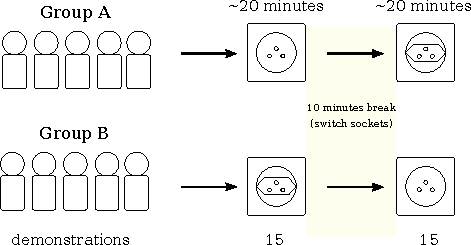
\includegraphics[width=0.8\textwidth]{./ch4-PiH/Figures/Fig/experiment_design_v2.pdf}
 \caption{Experiment protocol. The participants are divided in two groups of 5, Group A begins with socket A 
 and after a short break repeats the task with socket B. The same logic holds for Group B.
 For each socket 15 executions of the task are recorded.}
 \label{fig:experiment_design}
\end{figure}

%the usage of a chair as mentioned previously. The teachers were reminded that they were facing the direction of 
%the fake wall and that the starting location would be always within the orange rectangular area. 


\paragraph{Preliminary results}

Both groups A and B took $9\pm10$s to find the socket's edge, regardless of the socket type. This is to be expected since the sockets 
are at the same location. It took a further $8\pm7$s on average for group B to connect
socket B and $12\pm10$s on average for group A to connect socket A. As we can see this is not a straight forward task when considering
the sensory deprivation. See Figure \ref{fig:experiment_setup_data} (\textit{Bottom}) for the time taken to connect the plug to the socket.
In Appendix \ref{app:anova_socket} we report the results of an analyse of variance (ANOVA) on the time taken to connect
the sockets and we find that it takes 4 seconds more to connect socket A than socket B. This is somewhat expected as 
socket B has a funnel which can help to contain the subject to within the vicinity of the holes.

As connecting to socket A is more difficult we will \textbf{using only these demonstrations} as training data to learn a policy. Both
socket B and C will be used solely to evaluate the generalisation of the policy.

\begin{figure}
 \centering
   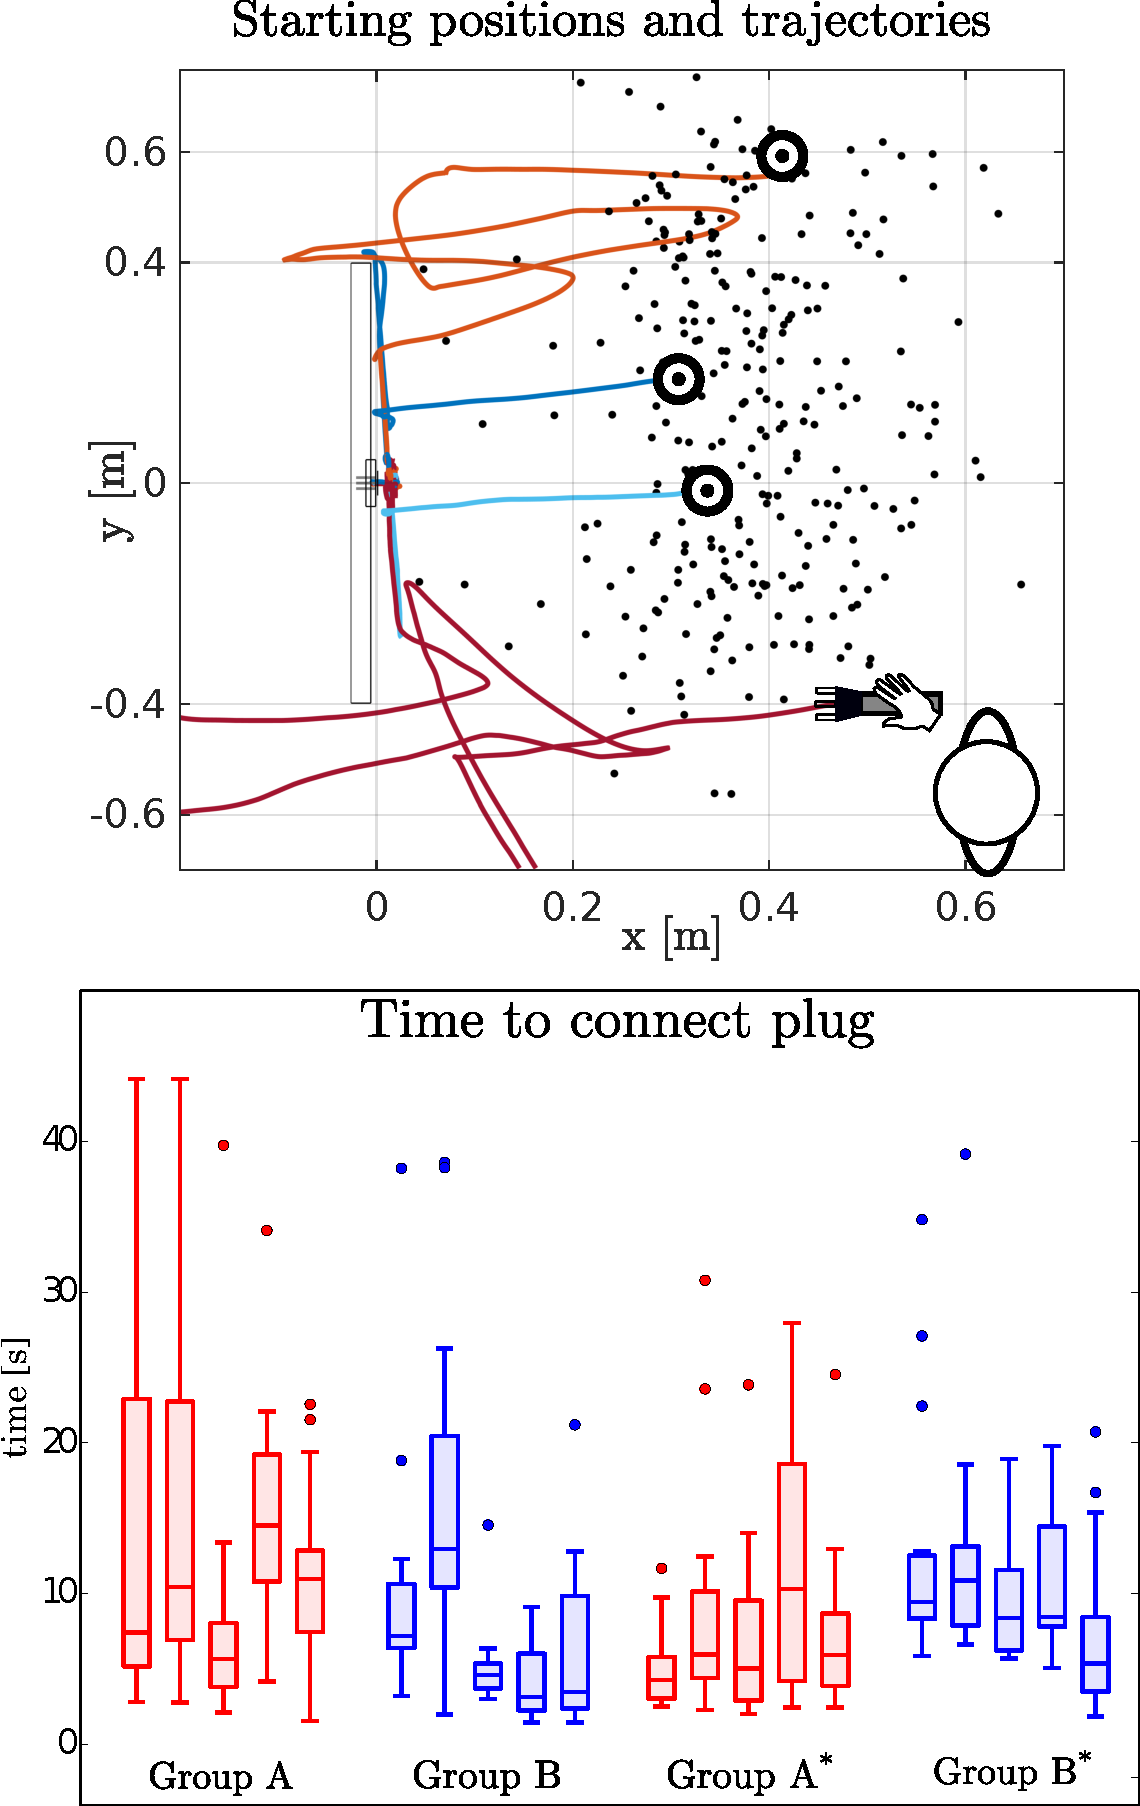
\includegraphics[width=\textwidth]{./ch4-PiH/Figures/Fig/start_position_v2.pdf}
   \caption{\textit{Top}: Black points represent the starting position of the end-effector
   for all the demonstrations. Four trajectories are illustrated. \textit{Bottom:} 
   Time taken for the teachers to accomplish the PiH once the socket is localised. Group A and B are depicted in red 
   and blue. The asterisk indicates that the group has changed sockets, so Group A\textsuperscript{*} means
   that Group A is now performing the task with socket B and Group B\textsuperscript{*} means that group B is now performing 
   the task with socket A.}
  \label{fig:experiment_setup_data}
\end{figure}

%In Figure \ref{fig:experiment_setup_data} we can see the time taken by the teachers to accomplish the task. 
%A group of 10 human teachers participated in the plug-socket experiment. Each teacher performed the search and PiH 
%for sockets A and B. A teacher of group A (starting with socket A), would start by performing 15 times the search and connection 
%with socket A and after a short break, during which socket A was replaced by socket B, would carry on to perform 15 trials 
%with socket B.

%The location belief of the humans was represented by a probability density function. We made the assumption 
%that after the disorientation step the human's believed location would be uniform and spread across the 
%rectangular starting area. Although the mental state of the human remains 
%unobservable, there is sufficient evidence to support our assumption that his belief state
%gets updated in a Bayesian fashion [citation].

\section{Learning Actor and Critic}\label{ch4:learning-value-actor}

In our approach we learn two data driven policies. The first policy maps from belief space 
to linear velocity $\pi_{\Param_1} : b_t \mapsto \dot{x}_t$ and the second from 
angular sensed wrench to angular velocity, $ \pi_{\Param_2} : \phi_t \mapsto \omega_t$.
We chose to learn the belief policy $\pi_{\Param_1}$ in a Actor-Critic RL framework 
and the wrench policy $\pi_{\Param_2}$ directly from the demonstrated data as was done 
in \cite[Chap. 5]{Kronander2015}, which proved to be efficient in overcoming jamming during the PiH. 
A POMDP solver's objective is to find a policy (Actor), $\pi_{\Param_1}: b \mapsto u$, which maximises 
the value function (Critic) $V^{\pi_{\Param_1}} : b \mapsto \mathbb{R}$ for an initial belief, $b_{0}$. The value function
is the expected reward over an infinite time horizon.
\begin{equation}\label{eq:value_function}
  V^{\pi_{\Param_1}}(b_t) = \mathbb{E}\Bigg\{ \sum_{t=0}^{\infty} \gamma^{t} r_{t+1} | b_0=b,\pi_{\Param_1}\Bigg\}
\end{equation}

In an Actor-Critic setting, the temporal difference error, $\delta_t \in \mathbb{R}$, of the value function (the Critic) is 
used as a learning signal to update simultaneously itself and the actor (the policy). In our method, 
two separate policies are learned, one for the linear velocity and the other for the angular velocity.
The orientation is kept constant until the start of the connection of the plug to the socket.
The angular velocity policy used and learned only during the insertion of the plug to the socket where it is necessary
to control the orientation to avoid jamming.

\subsection{Actor \& Critic}
%Two control policies are learned; The first $\pi_{\Param_1}: b \mapsto \U$, maps belief state $b$ to linear velocity, 
%$\U$ and the second, $\pi_{\Param_2}: \phi \mapsto \omega$ , sensed wrench, $\phi$, to angular velocity, $\omega$.
%These actors/policies are parametrised by a Gaussian Mixture Model (GMM), Equation \ref{eq:GMM}.
Both the linear and angular velocity policies are parameterised by a Gaussian Mixture Model (GMM), Equation \ref{eq:GMM}.

\begin{equation}
 \pi_{\Param}(\U,\B) = \sum\limits_{k=1}^{K} \piK	    \cdot  g(\U,\B;\MuK,\SigK) \label{eq:GMM}
\end{equation}
The parameters $\Param = \{w^{[k]},\MuK,\SigK\}_{1,\dots,K}$, are the weights, means and covariances 
of the individual Gaussian functions, $g(.)$,
\begin{center}
$\MuK =  \begin{bmatrix} \MuK_{\U} \\ \MuK_{\B} \end{bmatrix}$, 
$\SigK =  \begin{bmatrix} 
	  \SigK_{\U\U} & \SigK_{\U\B} \\
	  \SigK_{\B\U} & \SigK_{\B\B}
	  \end{bmatrix}$
\end{center}
where $\sum_{k} w^{[k]} = 1$, $\MuK_{\U} \in \mathbb{R}^{3}$ and  $\MuK_{\B} \in \mathbb{R}^{4}$.
%There are three steps to learning and use for control a GMM model.  Firstly a generative model is learned through 
%Expectation-Maximisation (EM) which maximised the likelihood

A generative model of the angular velocity and wrench $\pi_{\Param_2}(\omega,\theta)$ and a generative model 
of the linear velocity and belief state $\pi_{\Param_1}(\dot{x},b)$ are learned. 
In both cases we use the Bayesian Information Criterion to determine the number of Gaussian functions.
In the next section, we will show how the parameters of $\pi_{\Param_1}$ can be adapted by the value function of the Critic.

%First a generative model, $p_{\Param}(\dot{x},b)$, is learned through maximising the likelihood of 
%the dataset by Expectation-Maximisation (EM). 
%Second the conditional is taken $p_{\Param}(\dot{x}|b)$
%giving a distribution over the applicable actions $\dot{x}$, Equation \ref{eq:GMC}

%\begin{equation} 
%  \pi_{\Param}(\U|\B) = \sum\limits_{k=1}^{K} \piK(\B) \cdot  g(\B;\MuK_{\U|\B},\SigK_{\U|\B}) \label{eq:GMC}
%\end{equation}
%\begin{align}
% w^{[k]}(\B)  &= \frac{\piK \cdot g(\B;\MuK_{\B},\SigK_{\B\B})}{\sum_{j=1}^{K} w^{[j]} \cdot g(\B;\Mu{j}_{\B},\Sig{j}_{\B\B}) } \\
% \MuK_{\U|\B}   &= \MuK_{\U} + \SigK_{\U\B} \invSigK_{\B\B}(\B - \MuK_{\B})\\
%  \SigK_{\U|\B} &= \SigK_{\U\U} - \SigK_{\U\B}\invSigK_{\B\B}\SigK_{\B\U}
%\end{align}
%Thirdly a concrete action, to be applied, is derived from the conditional distribution. One approach is
%to take the expectation of the conditional, $\hat{\U} = \mathbb{E}_{p_{\Param}(\U|\B)}\{\U\}$ whilst 
%another is to draw a sample $\U \sim p_{\Param}(\U|\B)$. 


% Q-learning and TD(0) are based on the dynamic porgramming algorithm known as value iteration.
% 
%\cite{NIPS2008_3501} (Fitted Q-iteration by Advantage Weighted Regression)
%
%We use a combination of function approximation and dynamic programming to learn a value function 
%of the belief state with respect to the given task.

%\cite{Szepesvari:2010}

The Critic (the value function, Eq. \ref{eq:value_function}) evaluates 
the performance of the current policy. It is the expected future reward given the current 
belief state and policy.
In our method a reward of $r=0$ is received at each time step
until the goal (plug-socket connection) is achieved, where a reward of 100 is given, $r_{T}=100$.
Given the continuous nature and dimensionality of the belief space we use Locally Weighted Regression \cite{Atkeson97locallyweighted}
(LWR) as a function approximator of the value function, $V^{\pi}(b)$. LWR is a memory-based non-parametric function 
approximator. It keeps a set of input-target pairs $\{(\B,r)\}$ as parameters. When a value, $\B$, is 
queried, a set of $p$ neighbouring points are chosen from the input space and are 
weighted according to a distance metric. The predicted output is given by a weighted 
least square of the $p$ points. Equation \ref{eq:W} is the distance function used where 
$D$ is a diagonal matrix.

\begin{equation}\label{eq:W}
 W_{i,i}  = \exp\left(-\frac{1}{2}(\B - \B_i)^{\mathrm{T}}\, D^{-1} \, (\B - \B_i) \right)
\end{equation}
A new value is queried according to Equation \ref{eq:lwr_predict},
\begin{equation}\label{eq:lwr_predict}
  V^{\pi}(b) = \B \,(B^{\mathrm{T}} W B)^{-1} B^{\mathrm{T}} W \mathbf{r}
\end{equation}
where $B = (\B_1,\dots,\B_p)^{\mathrm{T}} \in \mathbb{R}^{(D\, \times\, p)}$, $W \in \mathbb{R}^{(p\, \times\, p)}$ is
a diagonal matrix, $\mathbf{r} = (r_1,\cdots,r_p)^{\mathrm{T}} \in \mathbb{R}^{(p\, \times\, 1)}$

%We chose this method because it is a safe regressor to use when estimating a value 
%function \cite{Boyan95generalizationin} and is very flexible since it is non-parameteric.

\subsection{Fitted policy evaluation and improvement}\label{sec:fpe}

\paragraph{Policy evaluation}\\

To learn the value function we make use of batch reinforcement learning \cite{EGW05}, also known as Experience replay.
This is an offline method which applies multiple sweeps of the Bellman backup operator 
over a dataset of tuples $\{(\Bi_t,\Ui_t,r^{[i]}_{t},\Bi_{t+1})\}_{i=1,\cdots,M}$ until the Bellman residual,
$||V^{\pi}_{k+1}(\B) - V^{\pi}_{k}(\B)||$, converges. 

\begin{center}
\begin{minipage}{.65\linewidth}
\begin{algorithm}[H]
\label{alg:fpe}
\SetKwInOut{Input}{input}
\SetKwInOut{Output}{output}
\Input{$\epsilon$, $\{(\B^{[i]}_t,r^{[i]},\B^{[i]}_{t+1})\}_{i=1,\cdots,M}$}
\Output{$\hat{V}^{\pi}_{k}(\B_t)$}
\BlankLine
\While{$||\hat{V}^{\pi}_{k+1}(\B) - \hat{V}^{\pi}_{k}(\B)|| < \epsilon$}{
  $\hat{V}^{\pi}_{k+1}(\B_t)$ = Regress($\B$, $r_t + \gamma \hat{V}^{\pi}_k(\B_{t+1}))$
}
\caption{Fitted Policy Evaluation}
\end{algorithm} 
\end{minipage}
\end{center}
Batch RL methods are used by a broad spectrum of research to learn policies. 
Most of them have focused on learning the Q-value function directly (Fitted Q-Iteration) 
\cite{NIPS2008_3501,EGW05,Riedmiller05neuralfitted}. Although this solves the control problem it requires discretisation 
of the action space or assumes quantifiable actions, as the 
Q-Bellman backups, $\hat{Q}(\B_t,\U_t) \leftarrow \gamma \max_{\U_{t+1}} \hat{Q}(\U_{t+1},\B_{t+1})$, 
require an optimisation over the action space, $\U_{t+1}$, to find the best applicable action. 
Given the dimensionality and continuity of our problem we opt for an on-policy evaluation method
which requires multiple \textit{policy evaluation} and \textit{policy improvement} iterations to achieve an optimal policy.
In order for the RL-PbD-POMDP and PbD-POMDP to be comparable we will only be performing one iteration of policy evaluation
and improvement, hence Algorithm \ref{alg:fpe} is applied only once to the dataset.
% Need to make clear we only do one iteration

%Which is not the case for Fitted Value Iteration (FVI) and Fitted Q-Iteration (FQI).
%After we applied the fitted policy evaluation to our dataset get the expected future 
%reward for each of the belief belief states, giving us a new dataset:
%$D = \big\{\U^{[i]}_{1:T},\omega^{[i]}_{1:T},\phi^{[i]}_{1:T},\B^{[i]}_{1:T},v^{[i]}_{1:T}\big\}^{i=1\dots N}$, where $v^{[i]}_t = \hat{V}^{\pi}(\Bi_t)$.
\paragraph{Policy improvement}\\
%\subsection{Policy improvement}

The Temporal Difference (TD) error $\delta^{\pi}_t = r_{t+1} + \gamma V^{\pi}(b_{t+1}) - V^{\pi}(b_t)$ 
given by the critic is used to update the actor  \cite[Chap. 6]{sutton1998reinforcement}. 
In our offline approach the value function of the belief state, $\hat{V}^{\pi}(\B)$, is estimated 
until convergence and then used to update the actor. This offline batch 
method has the advantage that no divergence can occur during the learning process.

We update the Actor policy given the Critic value function through a modification of the Maximisation step in  Expectation-Maximisation (EM) 
for Gaussian Mixture Models. We refer to this modification as Q-EM which is strongly related to a Monte-Carlo EM-based policy 
search approach \cite[p.50]{DeisenrothNP2013}. 

The reward of a demonstrated trajectory (one episode) is given by the discounted return, Equation $\ref{eq:disc_return}$.
\begin{equation}\label{eq:disc_return}
 R(\B^{[i]},\U^{[i]}) = \sum_{t=0}^{\mathrm{T^{[i]}}} \gamma^t \, r(\B^{[i]}_t,\U^{[i]}_t)
\end{equation}
All policy gradient approaches seek to find a set of parameters, $\Param$, of the Actor,
which will maximise the expected reward, equivalent to maximising Equation \ref{eq:expected_reward}.
\begin{align}\label{eq:expected_reward}
 J(\Param) &= \mathbb{E}_{\pi_{\Param}(\U,\B)}\{R(\B,\U)\} \nonumber \\
	  &= \sum\limits_{i=1}^{N}   \underbrace{\left( \prod_{t=0}^{T^{[i]}} \pi_{\Param}(\U^{[i]}_t,\B^{[i]}_t) \right)}_{\pi_{\Param}(\U^{[i]},\B^{[i]})} \, R(\B^{[i]},\U^{[i]}) 
\end{align}

To find the parameters which maximise the cost function, $\argmax_{\Param'} J(\Param')$, its derivative is set to zero. 
As this cannot be done directly, we maximise the logarithmic lower bound of the cost function which results in 
Equation \ref{eq:grad_log_cost}.

\begin{equation} \label{eq:grad_log_cost}
    \nabla_{\Param'}\log(J(\Param')) = \sum\limits_{i=1}^{N} \sum\limits_{t=0}^{T^{[i]}} \nabla_{\Param'}\log \pi_{\Param'}(\U^{[i]}_t,\B^{[i]}_t) \, Q^{\pi}(\U^{[i]}_t,\B^{[i]}_t)
\end{equation}

Setting the derivative of Equation \ref{eq:grad_log_cost} to zero and solving for the parameters
$\Param=\{w,\boldsymbol{\mu},\boldsymbol{\Sigma}\}$ leads to a Maximisation update step of EM
which is weighted by $Q^{\pi}$, see Appendix \ref{app:lb} for a more complete derivation.
We use the Critic's TD error as a substitute for $Q^{\pi}$. Assuming that our estimated value function, $\hat{V}^{\pi_{\Param}}$, 
is close to the true value function $V^{\pi_{\Param}}$, the TD error $\delta^{\pi}$ is an unbiased estimate of the advantage function, Equation \ref{eq:advantage_f} 
(see Appendix \ref{app:unbiased_delta}).
\begin{equation}\label{eq:advantage_f}
 A^{\pi}(b_t,u_t) = Q^{\pi}(b_t,u_t) - V^{\pi}(b_t) = \delta^{\pi}_t
\end{equation}
Using the advantage function as means of policy search is popular with methods such as
Natural Actor Critic (NAC) \cite{peter_nac_2008}.

Each data point has an associated weight, $\delta \in \mathbb{R}$, where $\delta^{[m]} \geq 0$ means that the 
state action-pair $\X^{[m]}$ leads to an increase in the value function and $\delta^{[m]} \leq 0$ leads to 
a decrease in the value function. The likelihood is re-weighted accordingly, giving more importance to data points which lead to a gain. Since 
the Q-EM update steps cannot allow negative weights, the TD error is rescaled to be between 0 and 1. % we already sed this

The reader is referred to Appendix \ref{app:grad} for the new Maximisation update step of Q-EM for a 
GMM parameterization of the policy.

%We learn the plug-socket search policy using the Q-EM update rules for a GMM parametrisation with the 
%data set, $D_1 = \big\{\U^{[i]}_{1:T},\B^{[i]}_{1:T},\delta^{[i]}_{1:T}\}^{i=1\dots N}$ and learn a second policy for inserting the 
%final steps of connecting the plug to socket with data set $D_2 = \{\omega^{[i]}_{1:T},\phi^{[i]}_{1:T}\}^{i=1\dots N}$. 
%In Figure \ref{fig:data_flow} we illustrate the data flow and the policies which are learned. Note that we also learn a belief space 
%policy directly from the demonstrations, $\pi_{\Param_3}(\U,\B)$, which we will refer to as the GMM policy and we will use it to compare 
%with the policy corrected by the Critic, which we call the Q-EM policy.
%\begin{figure}[h]
%  \centering
%  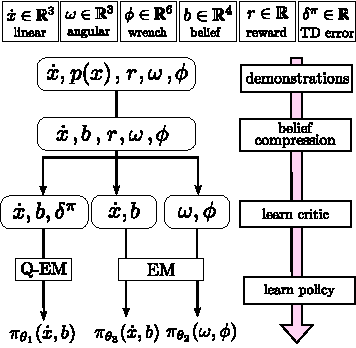
\includegraphics{Figures/data_flow_2.pdf}
%  \caption{Data flow and policies learned. The original data consists of five variables which are recorded during the demonstrations given 
%  by the human teachers. The probability density function of the believed location of the end effector is compressed to a belief state, which 
%  is the most likely state and entropy. The value function is learned via fitted policy iteration and each data point has a temporal difference 
%  error. An actor policy is learned via Q-EM, $\pi_{\Param_1}(\U,\B)$ , a regular policy is learned via the standard EM approach, $\pi_{\Param_3}(\U,\B)$
%  and a plug insertion policy is learned $\pi_{\Param_2}(\U,\B)$.}
%  \label{fig:data_flow}
%\end{figure}


%\subsection{Fitted policy evaluation and improvement}
\paragraph{2D example fitted policy evaluation and improvement}\\

To illustrate the mechanism of fitted policy evaluation and improvement, we give a 2D example 
of its application, see Figure \ref{fig:fpe_example}. The \textit{Top-left} subfigure
depicts 10 trajectories demonstrated by two teachers going from start (white circle) to goal (orange star) state. 
The optimal path is a straight line passing in between two obstacles. 
Neither teacher demonstrated the optimal straight path. 

In the \textit{Bottom-left}, a GMM is fitted $\pi_{\Param}(\U,\X)$ to the teachers' data, using the standard EM-algorithm.
Taking the policy to be the output of Gaussian Mixture Regression (GMR) $\mathbb{E}\{\pi_{\Param}(\U|\B)\}$ we obtain different
behaviours than those demonstrated by the human teachers. The GMR averages the different modes encoded by the Gaussian functions 
which results in a mixing of the original demonstrated behaviours. No trajectories of the GMR policy truly replicate 
the demonstrated behaviour. 

In the \textit{Top-right} subfigure, we apply fitted policy evaluation to the original demonstrated data (discount 
factor $\gamma=0.99$ and reward $r=1$ when the goal is reached and zero otherwise) and compute the value function.

The \textit{Bottom-right} subfigure illustrates the GMM policy learned with the Q-EM algorithm. As 
the advantage function $ A^{\pi}(\X,\U)$ is highest along the start-goal axis, data points
following this gradient will have a higher weight. This results in a policy with better 
rollouts (closer to the optimal path) than the trajectories generated by the policy learned via standard EM. 
%The \textit{Bottom-right} subfigure illustrates of 
%the Q-EM policy and rollout trajectories.

\begin{figure}
 \centering
 \setlength\fboxsep{0pt}
  \setlength\fboxrule{0.25pt}
  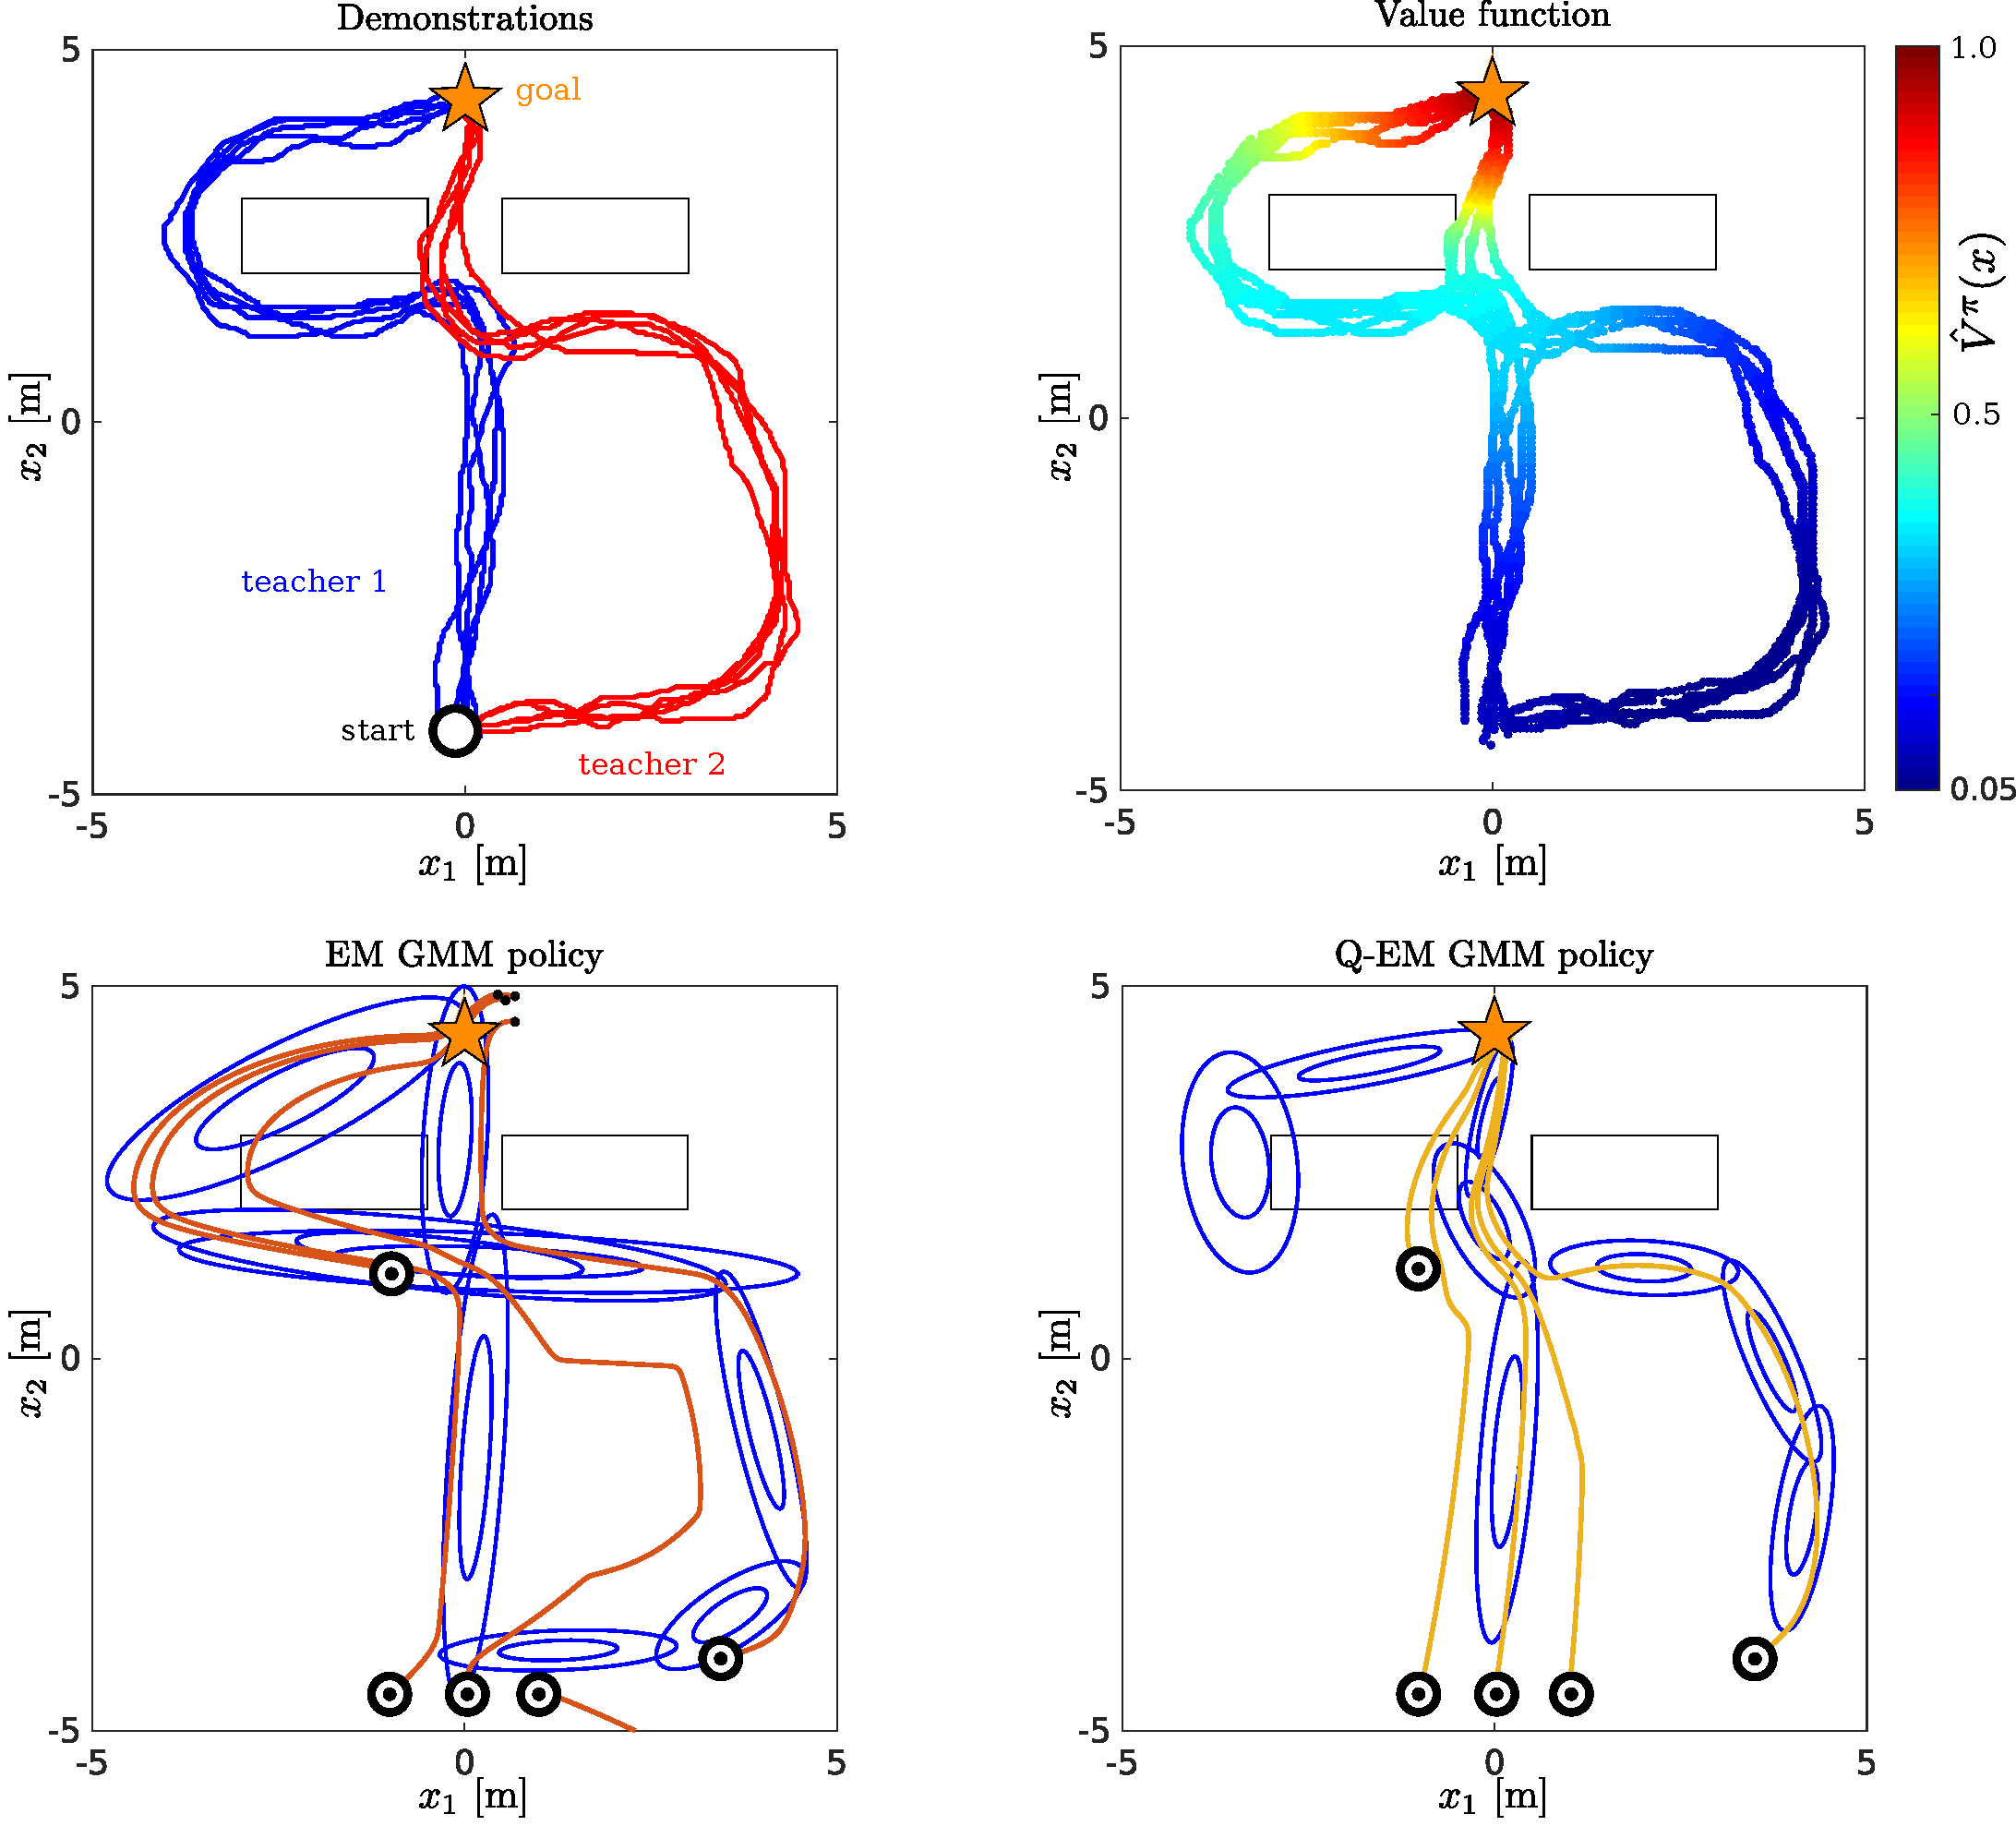
\includegraphics[width=\textwidth]{./ch4-PiH/Figures/fpe_example.pdf}
 \caption{Fitted policy evaluation \& improvement example. 
  \textit{Top-left:} The goal of the task is to reach the goal state. The first teacher (blue) demonstrates 
  five trajectories which contours the obstacle in front of the goal. The second teacher (red) demonstrates 
  5 trajectories which initially deviate from the goal before passing between the two obstacles. 
  \textit{Bottom-left:} The EM algorithm is used to fit a GMM to the teachers' original data. 
  The marginal $\pi_{\Param}(\X)$ is plotted in blue and trajectories generated by the 
  policy $\mathbb{E}\{\pi_{\Param}(\U|\X)\}$ in orange. \textit{Top-right} \textit{Policy Evaluation:}.  
  Value function after fitted policy evaluation terminated, the reward function 
  is binary, $r=1$ at the goal and zero otherwise, and a discount factor $\gamma = 0.99$ is used.
  \textit{Bottom-right} \textit{Policy Improvement:} the GMM is learned with the Q-EM algorithm in which 
  each data point's weight proportional to the advantage function.
 }
  \label{fig:fpe_example}
\end{figure}

\paragraph{Belief state fitted policy evaluation}

Returning to the PiH-search task with socket A, the Fitted Policy Evaluation (FPE) Algorithm \ref{alg:fpe} is applied to the 
demonstrations. In Figure \ref{fig:ch4:Figure1}  we illustrate the value function of the most likely state after the FPE algorithm converges. 
As expected, the value function is high closest to the socket and around the axis $z=0$ and $y=0$. 
When policy improvement via Q-EM is applied the Gaussian functions of the GMM will favour these locations. 

\begin{figure}
 \centering
 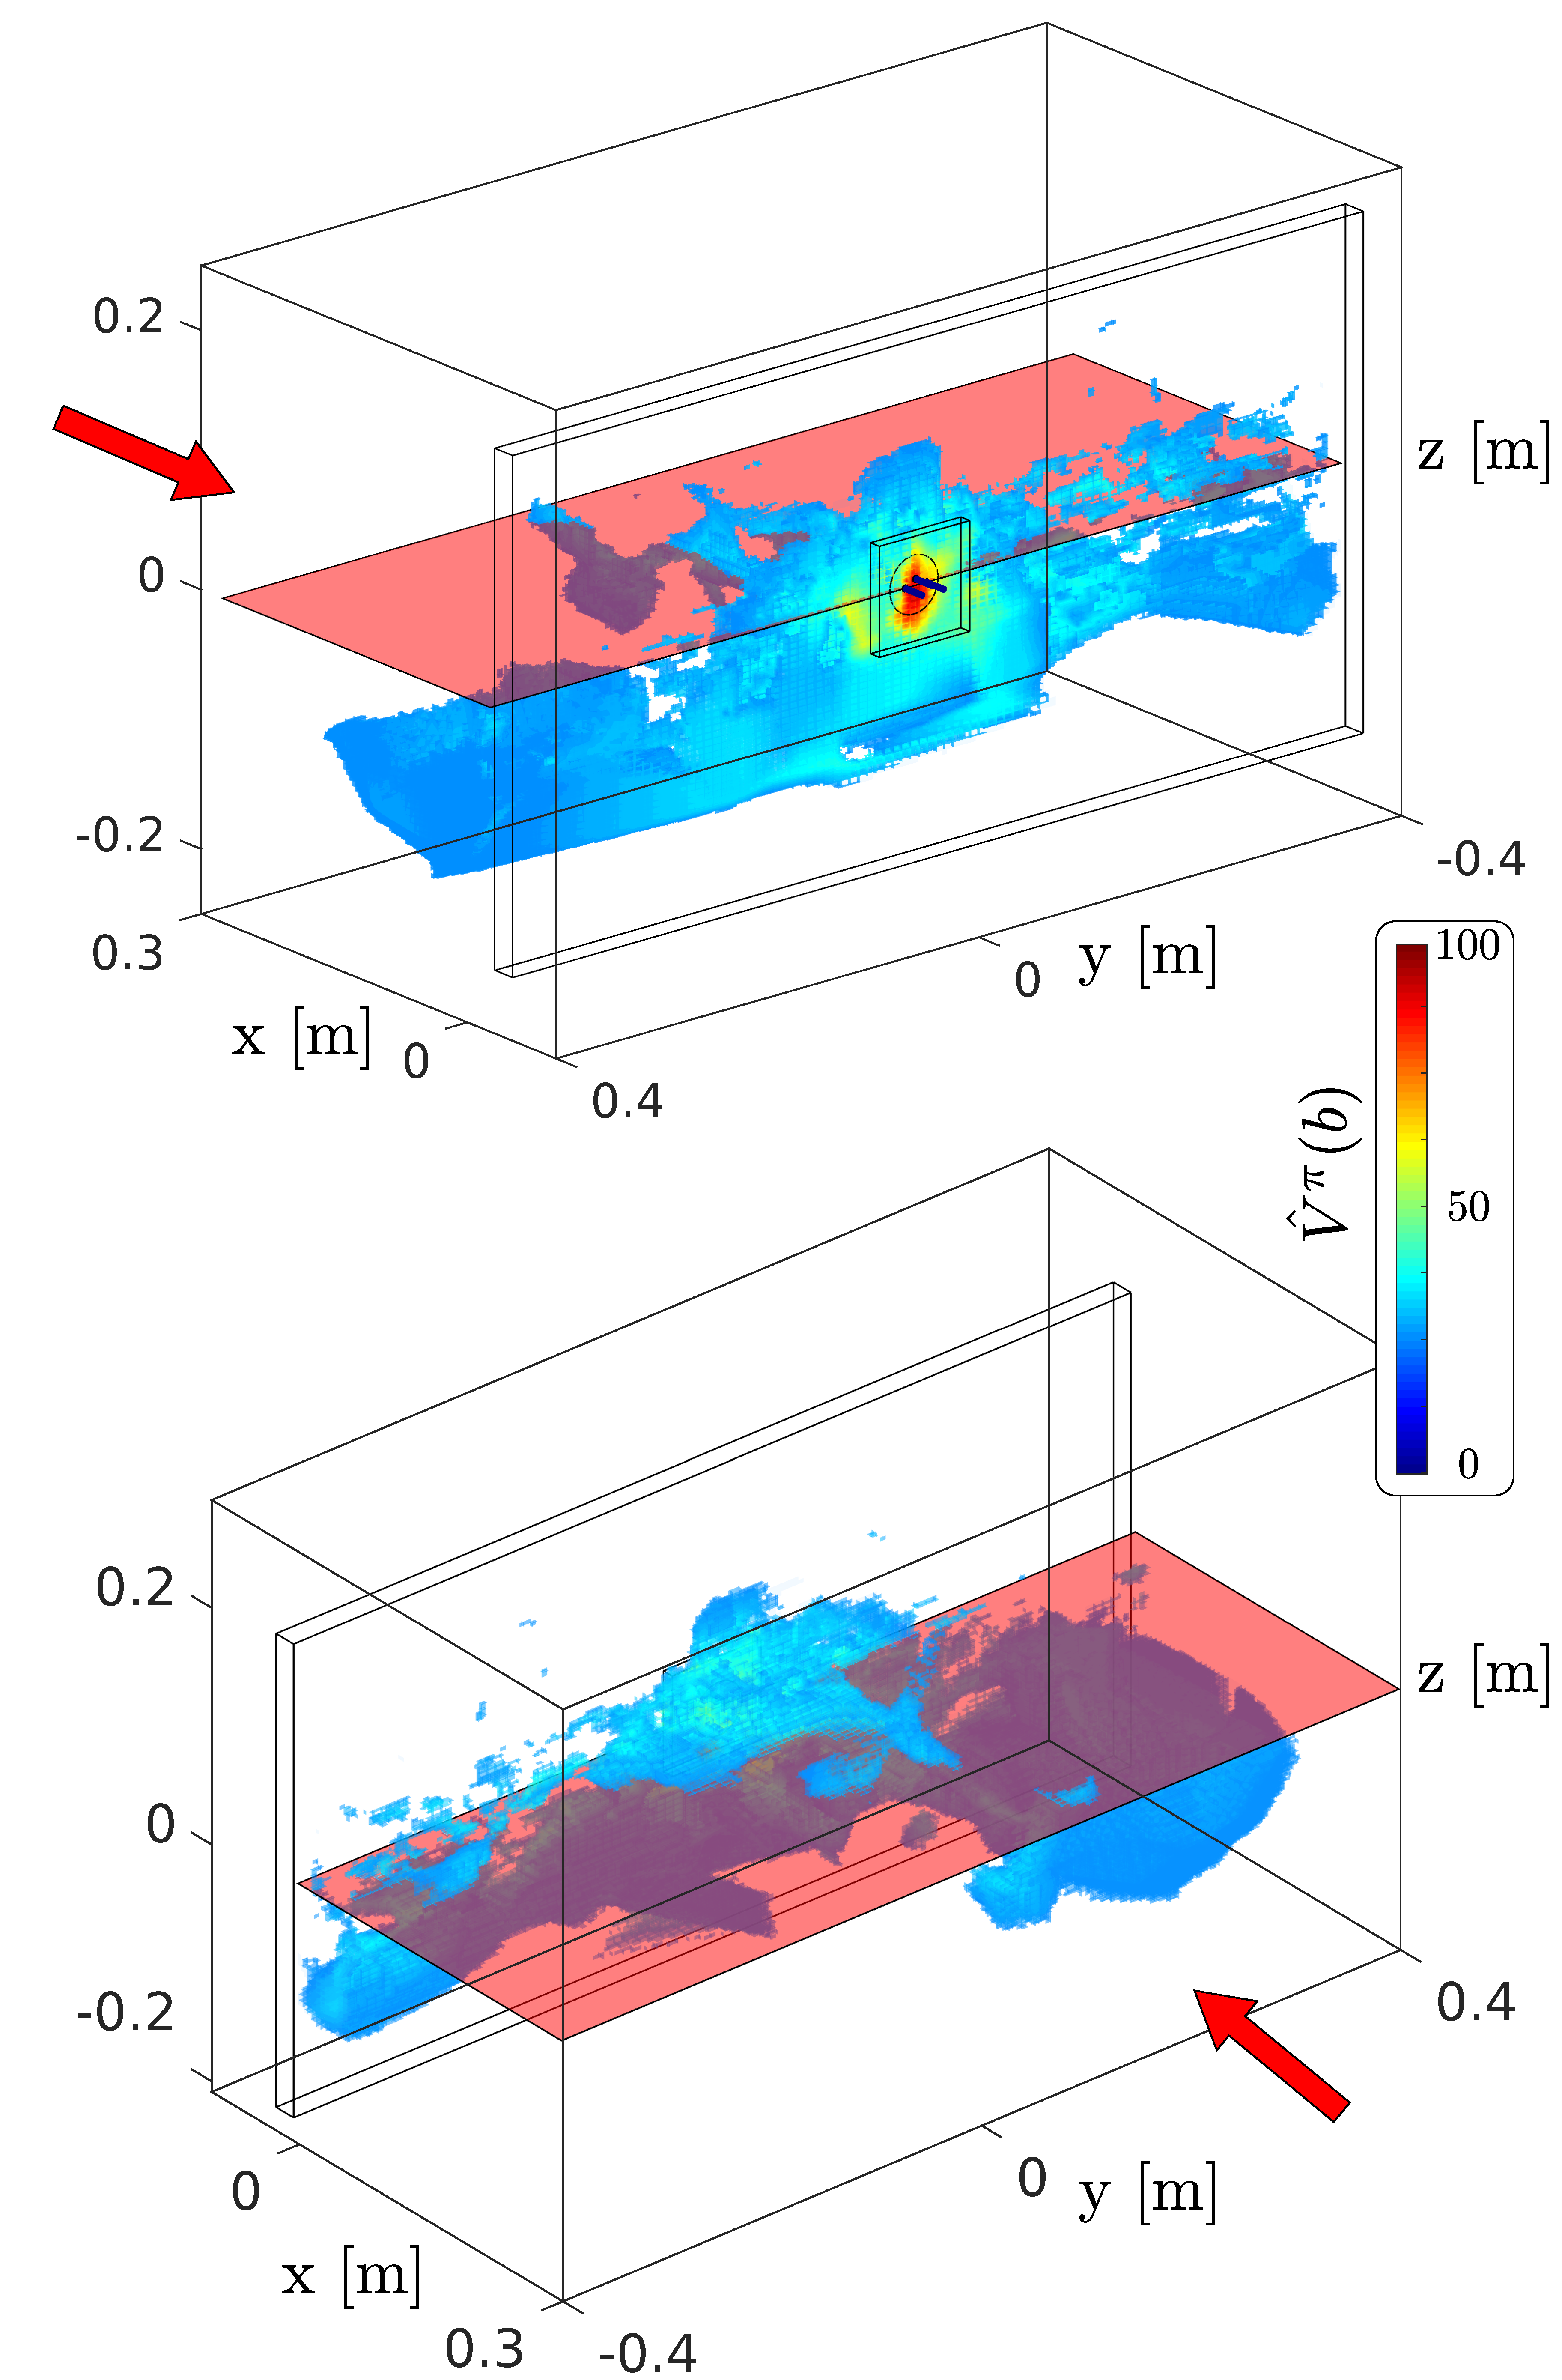
\includegraphics[width=\textwidth]{./ch4-PiH/Figures/ValueFunction/value_func_final_v2.pdf}
 \caption{LWR value function approximate $\hat{V}^{\pi}(\hat{x})$ for the most likely state $\hat{x}$. 
 The red plane is to help visualise where the value function is above and below the axis $z=0$. Only states with values above
 $0.25$ are plotted.  The red arrow indicates the heading of the human teacher when performing the search task. The discount 
 factor was $\gamma=0.99$ and the variance of the kernel variance of 1 [cm], which was set experimentally.
}
 \label{fig:ch4:Figure1}
\end{figure}

In Figure \ref{fig:best_worst_traj} we illustrate the best and worst trajectories in terms of the accumulated value function.
We can see that the five best trajectories (red) tend to be aligned with the socket (star position in front of socket), 
whilst the worst trajectories are towards the edges of the wall and tend to follow spiralling movements. 

\begin{figure}
 \centering
 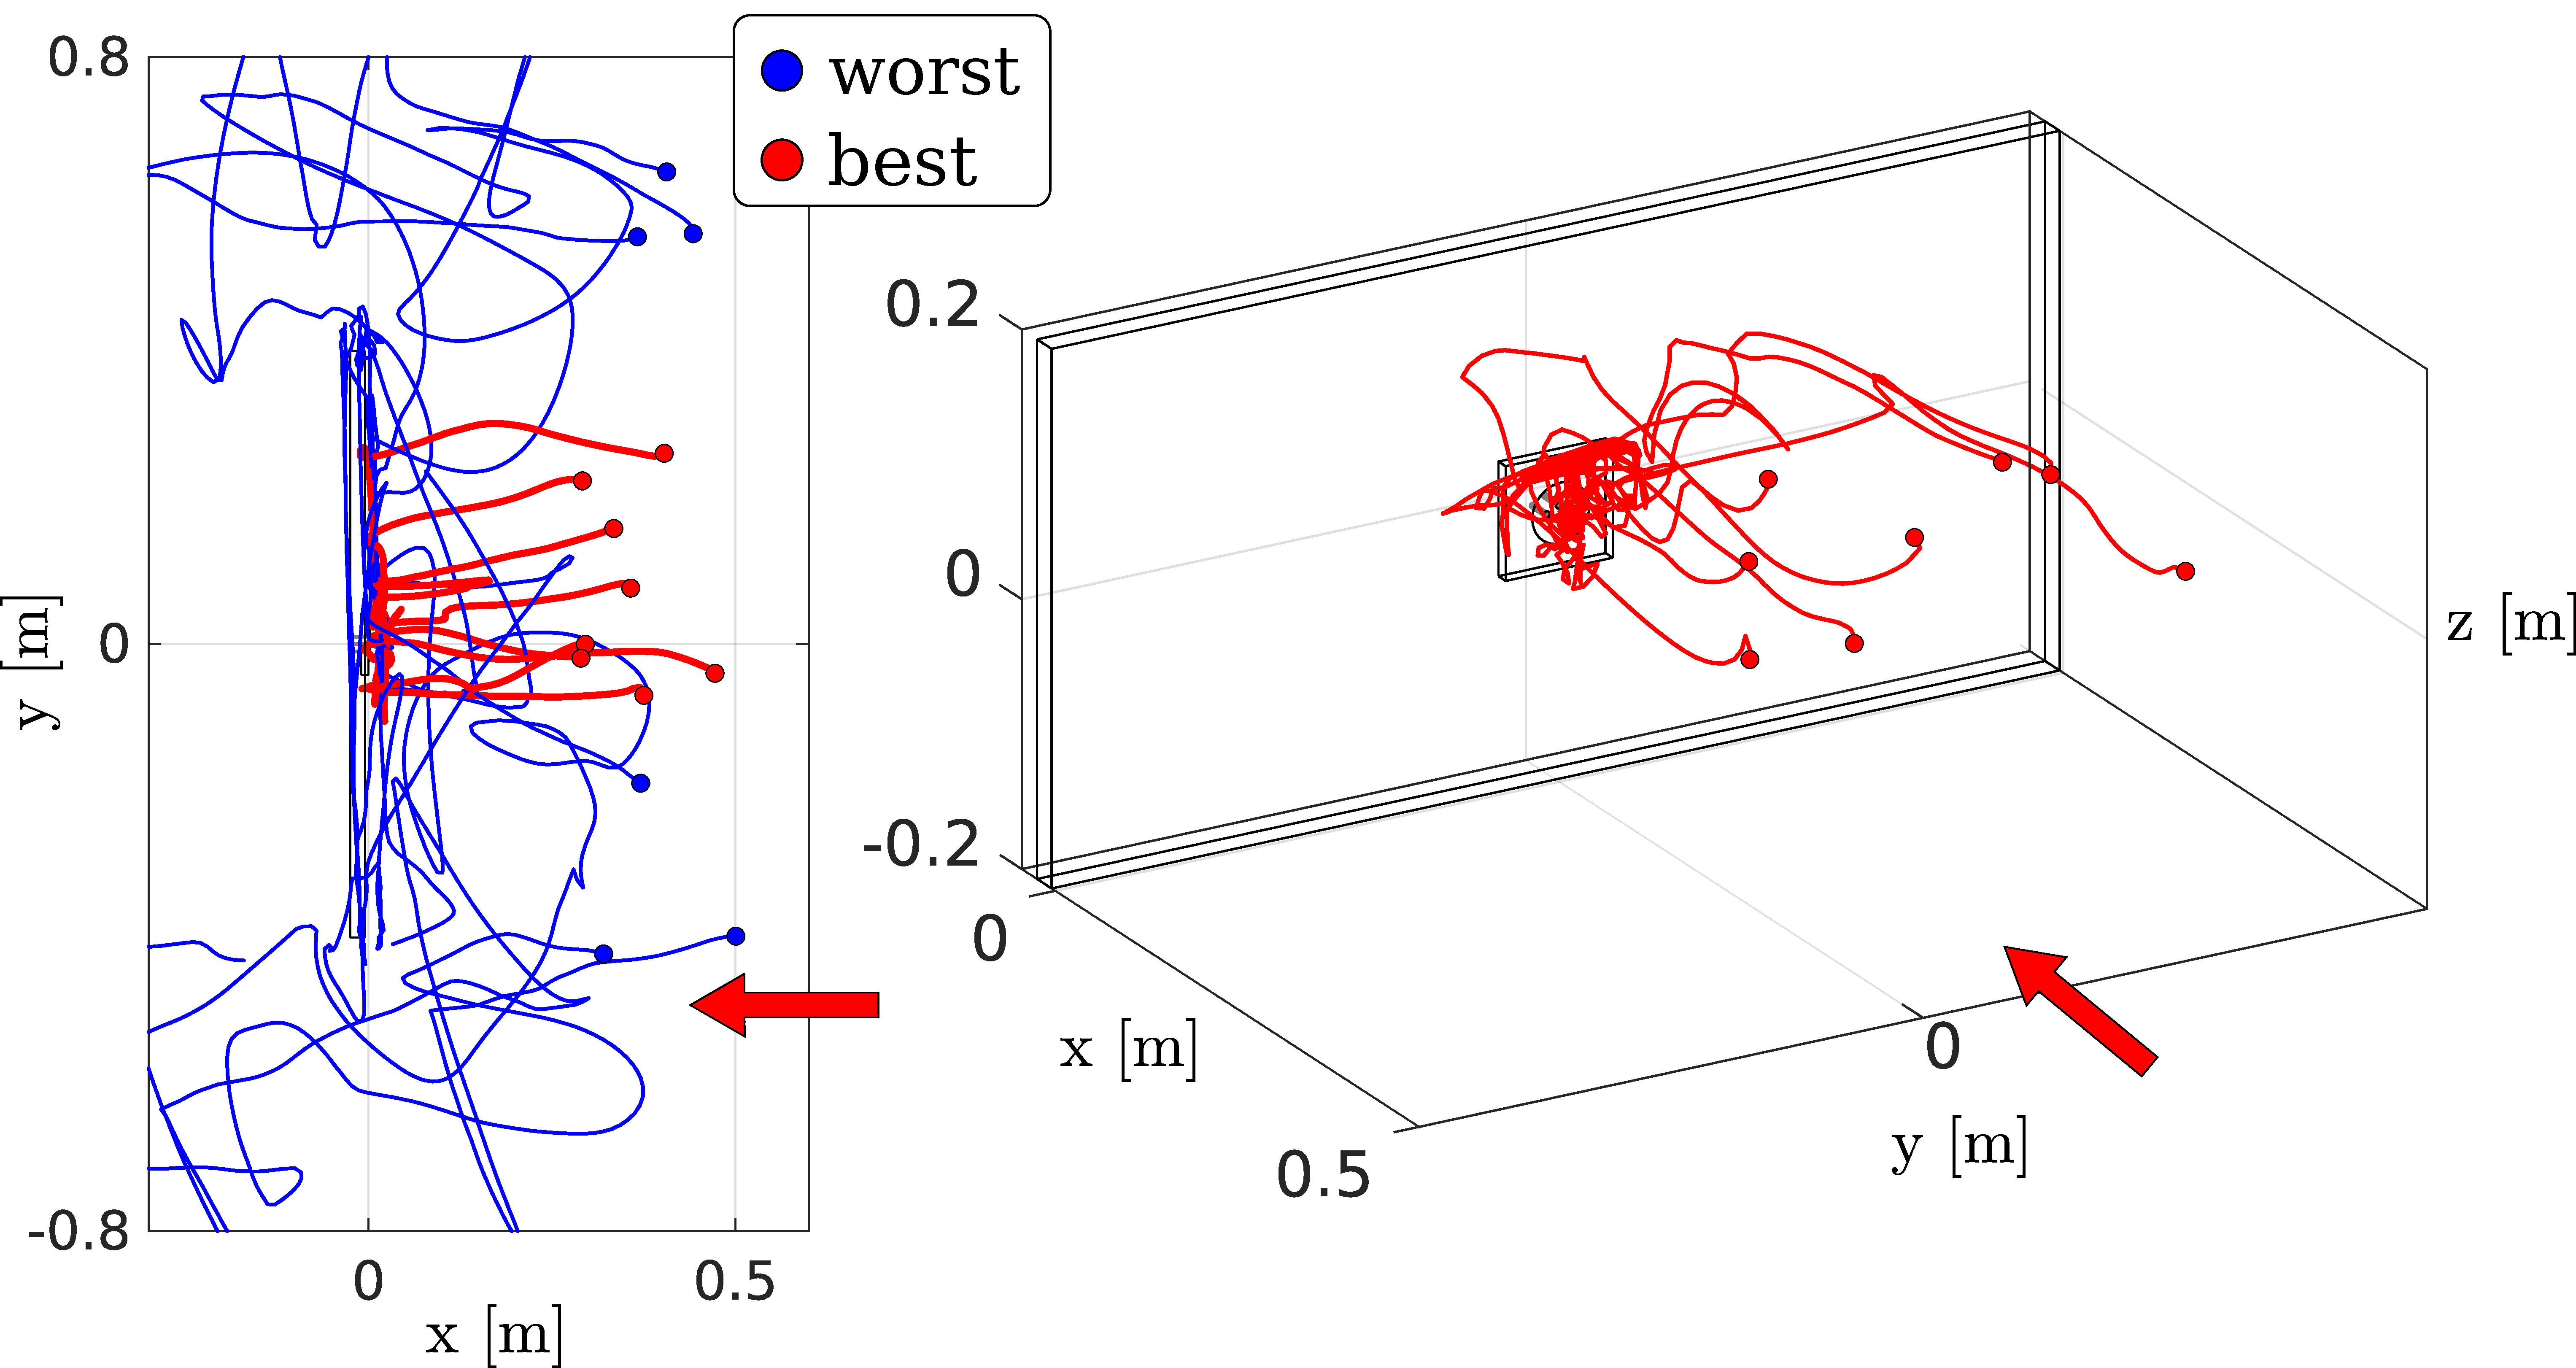
\includegraphics[width=\textwidth]{./ch4-PiH/Figures/ValueFunction/value_func_final_v3.pdf}
 \caption{Best and worst trajectories. The red demonstrated trajectories are the best in terms of the amount of value function 
 gain whilst the blue are the worst. The red arrow indicates the teacher's heading. The blue trajectories tend 
 towards the sides of the wall as the initial starting position is on the boarders of the wall. The red trajectories are centred along the y-axis of socket and tend to move in a straight line towards 
 the wall whilst aligning themselves with the axis $z=0$.} 
 \label{fig:best_worst_traj}
\end{figure}


We learned two policies, one solely from the original human demonstrations which we call GMM and the second which 
is the result of one iteration of fitted policy evaluation and improvement which we call Q-EM. In the section \ref{ch4:results}
we compare the GMM and Q-EM policies with the improvements which can be achieved within the RL-PbD-POMDP framework.

\section{Control architecture}\label{ch4:control_architecture}

As detailed in section \ref{sec:fpe}, a Gaussian Mixture Model was learned for both linear and angular velocity,
although only the linear control policy is active until the plug is within 
the socket's hole, as the orientation is constant.
The direction to search is given by the conditional, Equation \ref{eq:gmm_conditional},

\begin{equation}\label{eq:gmm_conditional}
 \pi_{\Param}(\dot{x}|b) = \sum_{k=1}^{K} w^{[k]}_{\xb} \cdot g(\dot{x};\MuK_{\xb},\SigK_{\xb}) 
 \end{equation}

which is a distribution over the possible normalised velocities. The function $g(\cdot)$ is a multivariate
Gaussian function parameterised by mean $\MuK_{\xb} \in \mathbb{R}^{(3\times1)}$ and Covariance $\SigK_{\xb} \in \mathbb{R}^{(3\times3)}$. The subscript $\xb$ indicates that the parameters 
are the result of the conditional. The reader is referred to \cite{gesture_calinon_2010}, \cite{gmr_2004} for 
a detailed derivation of the conditional of a GMM. The learned model 
is multi-modal, as different search velocities are possible 
in the same belief state. Figure \ref{fig:policy_vf} illustrates the multi-modal 
vector fields of the conditional, Equation \ref{eq:gmm_conditional}.
In autonomous dynamical systems control, the velocity is obtained from 
the expectation of the conditional, Equation \ref{eq:gmm_conditional}. However, the expectation which is a weighted 
linear combination of the modes, could result in unobserved behaviour or no movement if the velocities cancel out. 
As a result we use a modified version of the expectation operator which favours the current
direction, Equation \ref{eq:alpha_eq} - \ref{eq:alpha_expectation}.

\begin{align}
 \alpha(\dot{x}) &= w^{[k]}_{\xb} \cdot \exp(-\cos^{-1}(<\dot{x},\MuK_{\xb}>)) \label{eq:alpha_eq}\\
 \dot{x} &= \mathbb{E}_{\alpha}\{\pi_{\Param}(\dot{x}|b)\} = \sum_{k=1}^K \alpha_k(\dot{x}) \cdot \MuK_{\xb} \label{eq:alpha_expectation}
\end{align}

When the applied velocity mode is no longer present another direction is sampled. For example, when the robot enters in contact 
with a feature, greatly reducing the uncertainty, the current mode changes and a new search direction is computed. 
Figure \ref{fig:policy_vf} illustrates the policy vector field for GMM and Q-EM, both learned from teachers demonstrations.

\begin{figure}
   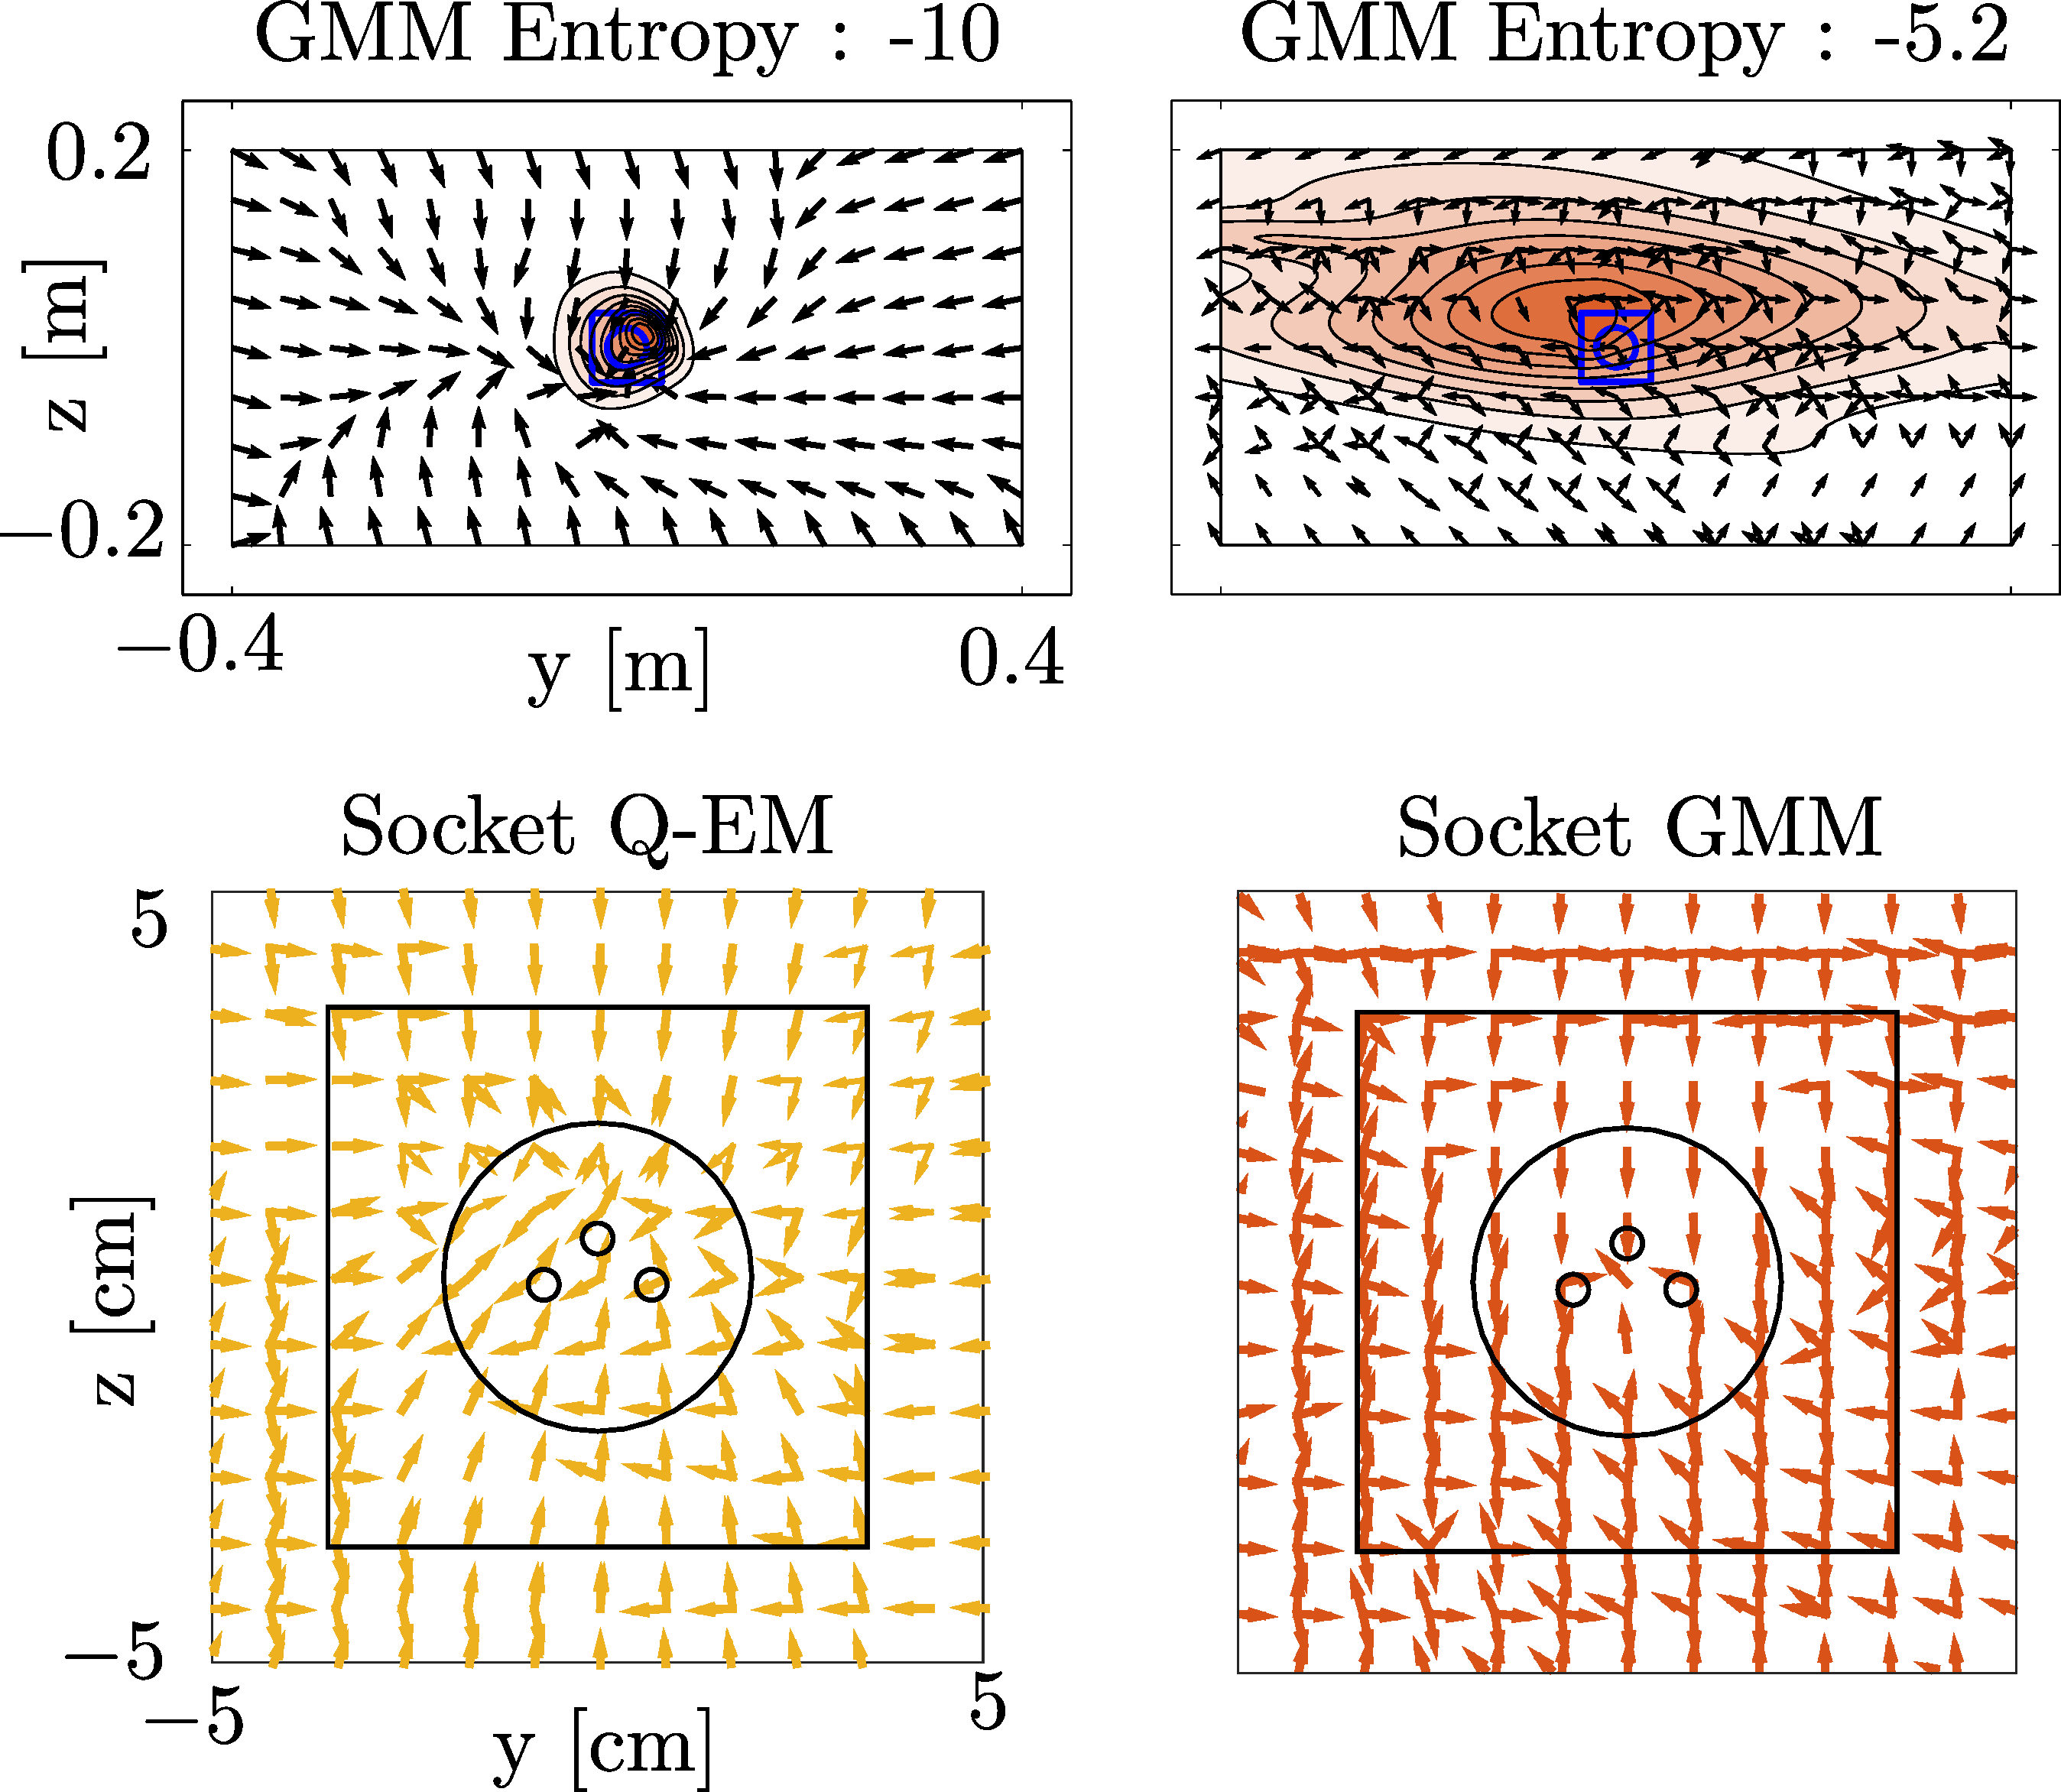
\includegraphics[width=\textwidth]{./ch4-PiH/Figures/Fig/policy_vf.pdf}
  \caption{Q-EM and GMM policy vector fields. \textit{Top}: The GMM policy is conditioned on an entropy of $-10$ and $-5.2$. For the lowest entropy level,
  most of the probability mass is close to the socket area since this level corresponds to very little uncertainty; we are already localised. We can see 
  that the policy converges to the socket area regardless of the location of the believed state. For an entropy of $-5.2$ we can see that 
  the likelihood of the policy is present across wall. The vector field directs the end-effector to go towards the left or right edge of the wall. 
  \textit{Bottom}: The entropy is marginalised out, the yellow vector field is of the Q-EM and orange of the GMM. The Q-EM vector field tends 
  to be closer to a sink and there is less variation.}
  \label{fig:policy_vf}
\end{figure}


\subsection{Robot Implementation}

The GMM policy $\dot{\underbar{x}} = \mathbb{E}_{\alpha}\{\pi_{\Param}(\dot{x}|b)\}$ outputs a linear velocity which is normalised, $\dot{\underbar{x}} \in \mathbb{R}^{(3 \times 1)}$. 
The amplitude of the velocity is computed separately and modulated according to sensed forces on the end-effector.
This search task is haptic and the end-effector of the robot is always in contact with the environment. To make the robot
compliant with the environment we use an impedance controller in combination with a hybrid position-force controller. A hybrid controller
targets a sensed force $F_x$, in the $x$-axis, of 3N. The $y$ and $z$ velocity components of the direction vector are given by 
Equation \ref{eq:alpha_expectation}. This is insufficient for the robot to reliably surmount the edges of the socket,
hence the vector field of the GMM is modulated in $y$ and $z$-axis, Equation \ref{eq:modulation}.

\begin{equation}
  \dot{\underbar{x}} = R_y(c(F_z) \cdot \pi/2) \cdot R_z(c(F_y) \cdot \pi/2) \cdot \dot{\underbar{x}} \label{eq:modulation}
\end{equation}

where $R_y$ and $R_z$ are $(3 \times 3)$ rotation matrices around the $y$ and $z$-axis, and $c(F) \in [-1,1]$ is a truncated scaling function of the sensed 
force.  When a force $F_z$ of 5N is sensed, a rotation of $R_y(\pi/2)$ is applied to the original direction resulting in the robot
getting over the edge. The direction velocity is always normalised up to this point. The amplitude of the velocity is a proportional
controller based on the believed distance to the goal,
\begin{align}
  \nu     &= \max(\min(\beta_1,K_p (x_g - \hat{x}),\beta_2)\label{eq:prop_speed}\\ \nonumber
  \dot{x} &= \nu \dot{\underbar{x}}
\end{align}
where the lower and upper amplitude limits are given by $\beta_1$ and $\beta_2$, $x_g$ is the position of the
goal, and $K_p$ the proportional gain which was tuned through trials. 

The above procedure can control the general behaviour of the search but is insufficient for a successful implementation on a robotic system 
such as the 7 Degree of Freedom $q\in\mathbb{R}^7$ KUKA LWR, which we illustrate in Figure \ref{fig:kuka}. 
The GMM policy $\dot{x} = \mathbb{E}_{\alpha}\{\pi_{\Param_1}(\dot{x}|b)\}$ outputs a linear velocity and the 
angular velocity $\omega_t = \mathrm{angleaxis}(\mathbf{R}^{\mathrm{T}} \mathbf{R}^r)$ is computed from a 
reference orientation $\mathbf{R}^r = I$ which is constant. When the plug is to be connected to the socket, 
the angular velocity is the output of samples drawn from the conditional $\omega \sim \pi_{\Param_2}(\omega|\phi)$.
Given the kinematic chain of the robot, the inverse of the Jacobian $J(q) \in \mathbb{R}^{6\times 7}$ is used in an impedance control to transform the 
Cartesian control $u_t = [\dot{x}_t,\omega_t]^{\mathrm{T}}$ to torque commands $\tau_t \in \mathbb{R}^7$, Equation \ref{eq:torque_control},

\begin{equation}\label{eq:torque_control}
 \tau_t = J^{\mathrm{T}}(q_t)\left(-K u_t - D \dot{u}_t \right) + g(q)
\end{equation}

where $K,D \in \mathbb{R}^{6\times6}$ are diagonal stiffness and damping matrices and $g(q)$ compensates for gravity. Given an applied torque there is 
a resulting joint velocity $\dot{q}_t$ from which we can compute the measured Cartesian end-effector velocity used in the motion model of the PMF.
Figure \ref{fig:control_flow} illustrates the complete control flow.

\begin{figure}
 \centering
 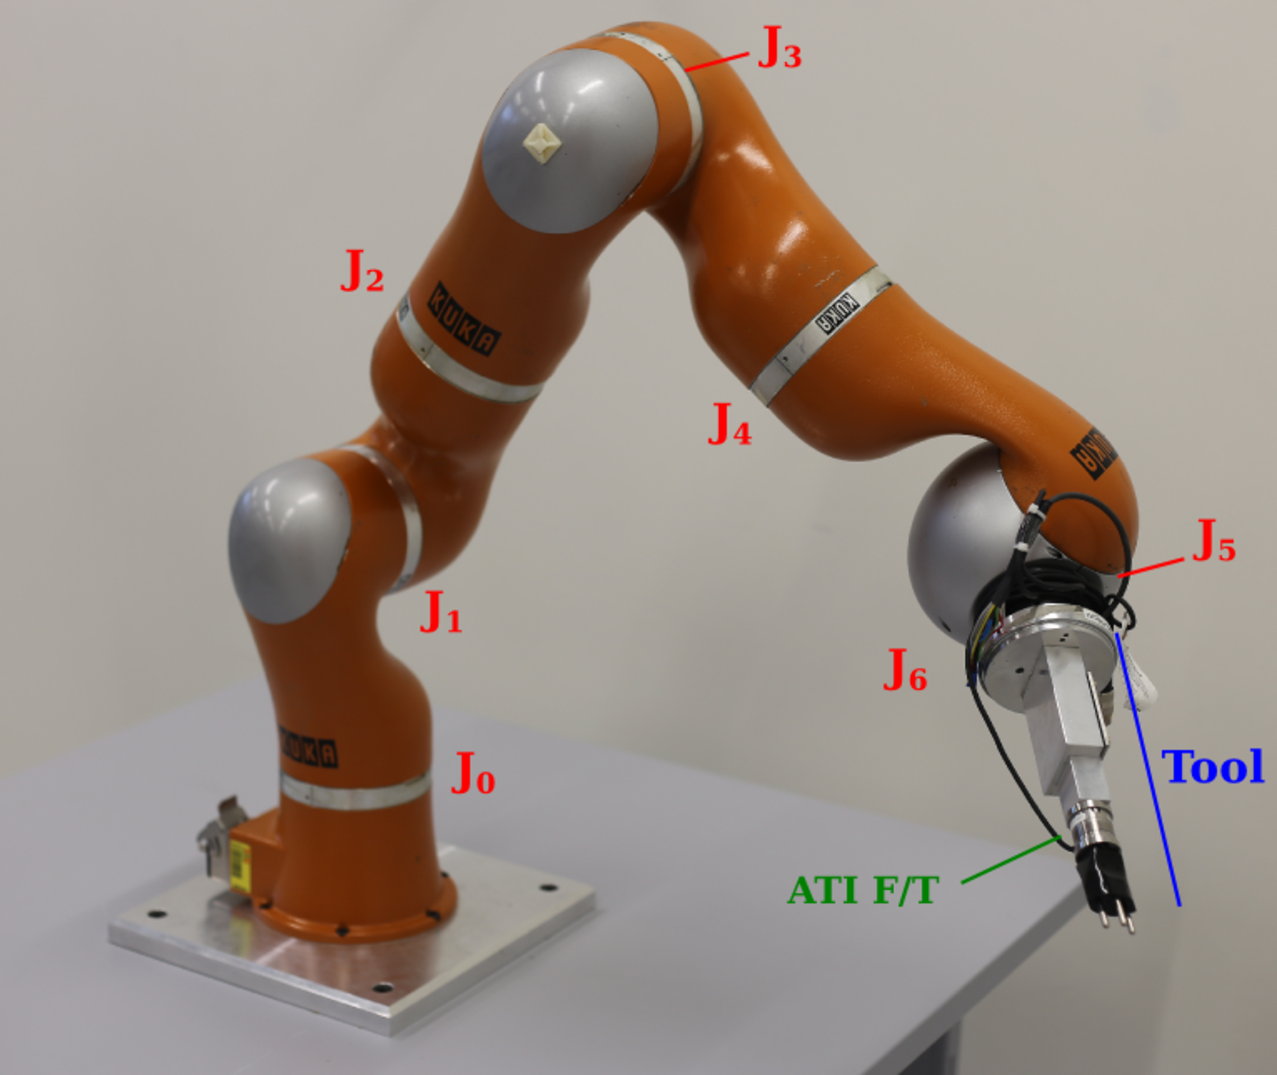
\includegraphics[width=0.8\textwidth]{./ch4-PiH/Figures/kuka.pdf}
 \caption{The KUKA LWR is a 7 Degree Of Freedom (DoF) robot, we illustrate in red each joint, which is controlled at a rate of 1kHz via an ethernet cable. The KUKA API provides a command interface to the 
 stiffness, damping, position and torque variables of each joint.}
 \label{fig:kuka}
\end{figure}

\begin{figure}
  \centering
  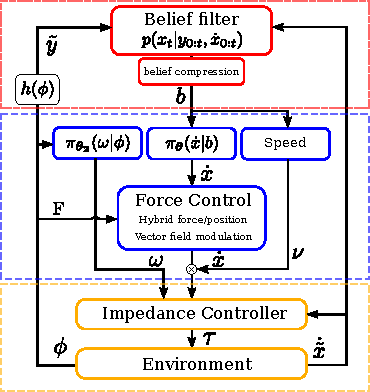
\includegraphics[width=0.8\textwidth]{./ch4-PiH/Figures/control_flow_final.pdf}
  \caption{Control architecture. The PMF (belief) receives a measured velocity, $\dot{\tilde{x}}$, and 
  a sensor measurement $\tilde{y}$ and is updated via Bayes rule. The belief is compressed and used by both the GMM policy and the proportional speed controller, Equation \ref{eq:prop_speed}.}
  \label{fig:control_flow}
\end{figure}


\FloatBarrier
\section{Results}\label{ch4:results}

We evaluate the following three aspects of the policy learned in our Actor-Critic framework:
\begin{enumerate}
 \item \textbf{Distance taken to accomplish the goal} (connect plug to socket). We compare the Q-EM policy with 
 a GMM policy learned through standard EM and a myopic Greedy policy. This highlights the difference between complicated and simplistic  
  search algorithms and gives an appreciation of the problem's difficulty.
 \item \textbf{Importance of data} provided by human teachers. We evaluate whether it is possible to learn 
 an improved GMM policy from Greedy demonstrations. This policy which we call Q-Greedy is used to test whether 
 indeed human demonstrations are necessary.
 We evaluate whether it is possible to obtain a good policy from the two worst teachers' demonstrations as not all teachers 
 are necessarily proficient at the task in question and we want to test whether our methodology can be applied in these
 cases. We evaluate if we  are able to obtain an improved policy from the worst two teachers.
 \item \textbf{Generalisation}. We learn a policy to insert a plug into socket A which is located at the center of a wooden 
 wall. We test the generalisation of the policy in finding a new socket location and whether the policy can generalise to sockets 
 B and C, which were not used during the training phase.
\end{enumerate}

We evaluate the above properties under two separate conditions. In the \textbf{first condition} we consider the period between the start 
of the search until the socket is localised. In the \textbf{second condition} we consider the period from the point the socket is found until
a connection has been established. In the first condition the evaluation is done in simulation whilst 
in the second condition, when the socket is found, we perform the evaluation with a physical robot, the KUKA LWR4.

This choice is motivated by the fact that the two parts of the task require different levels of precision.
Finding the socket requires much less precision than establishing a connection. It is more informative to consider the performance of these two parts separately.
Another aspect is that the search for the socket can be reliably evaluated in simulation since the physics of the interaction
is simple. The connection phase is more complicated and a simulation would be unrealistic.
For the evaluation of the connection of the plug to the socket we consider the search start point already within 
the vicinity of the socket.

\subsection{Distance taken to reach the socket's edge (Qualitative)}

We consider three search experiments which we refer to as \textbf{Experiment 1, 2} and \textbf{3},
in order to evaluate the performance in terms of the distance travelled to reach the socket for the three search policies: GMM, Q-EM and Greedy.
In these three experiments the task is considered accomplished when a search policy finds the socket's edge. 

In \textbf{Experiment 1}, three starting locations are chosen: \textit{Center}, \textit{Left} and \textit{Right}. 
See Figure \ref{fig:box_exp_sim}, \textit{Experiment 1}, for an illustration of the initial condition. 
This setup tests the effect of the starting positions. A total of 25 searches are carried out for each of the search policies.

In \textbf{Experiment 2}, two \textit{Cases} are chosen in which the believed state (most likely state of the PMF) and the true position
of the end-effector are relatively far apart. The location of the beliefs are chosen to be symmetric, see the Figure \ref{fig:box_exp_sim}, 
\textit{Experiment 2}. A total of 25 searches are carried for each of the two cases.

In \textbf{Experiment 3}, Figure \ref{fig:box_exp_sim}, \textit{Experiment 3}, the initial true starting positions 
of the end-effector are taken from a regular grid covering the whole start region, also used as the initial distribution for 
the human demonstrations. A total of a 150 searches are carried out for each of the three policies. 
This experiment compares the search policies with the human teachers' demonstrations.

\begin{figure}
    \centering
    \hspace*{-1.4cm}
    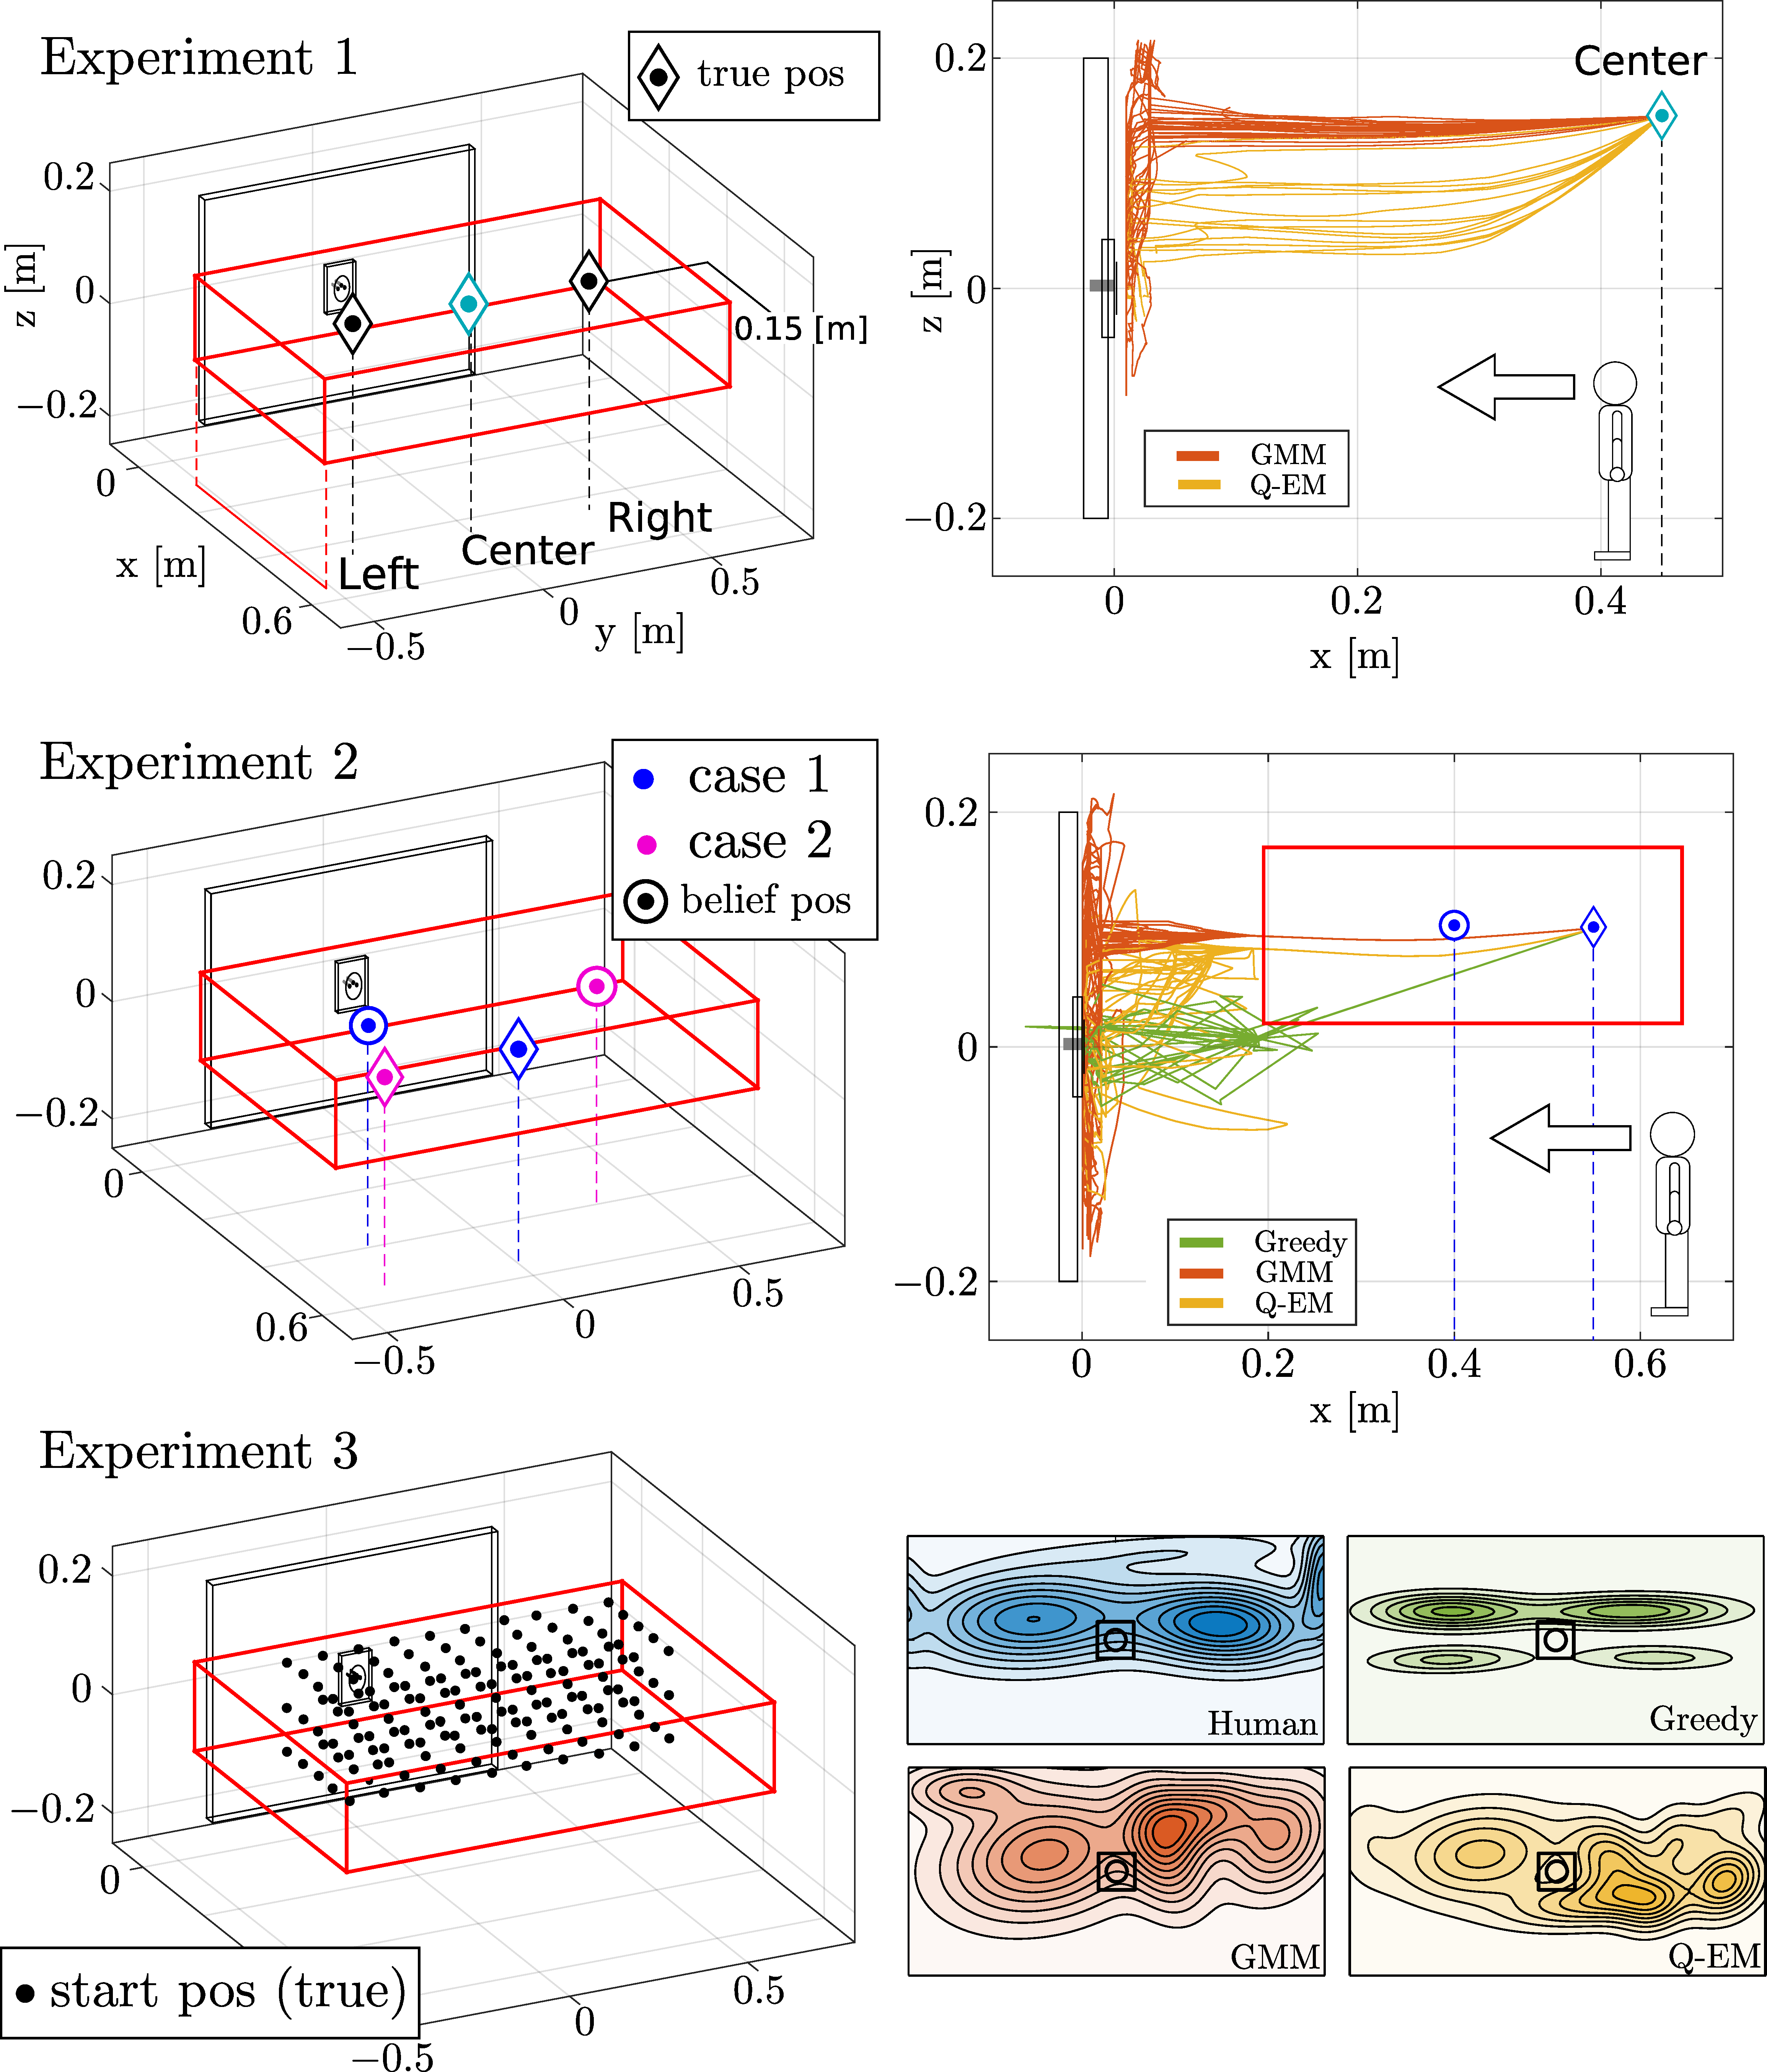
\includegraphics[width=1.2\textwidth]{./ch4-PiH/Figures/Fig/experiment_final_v3.pdf}
    \caption{Three simulated search experiments. \textbf{Experiment 1:} Three start positions are considered: \textit{Left}, \textit{Center} and
     \textit{Right} in which the triangles depict true position of the end-effector. The red cube illustrates the extent of the uncertainty. 
     In the second row of Experiment 1, we illustrate the trajectories of both the GMM (orange) and Q-EM (yellow) policies. For each start condition 
     a total of 25 searches were performed for each search policy. 
     \textbf{Experiment 2:} Two cases are considered: \textit{Case 1} blue, the initial belief state (circle) is fixed facing 
     the left edge of the wall and the true location (diamond) is facing the socket.
     \textit{Case 2} pink, the initial belief state (circle) is fixed to the right facing the edge of the wall and the 
     true location is the left edge of the wall. In the second row, the trajectories are plotted for \textit{Case 1}.
     \textbf{Experiment 3:} A 150 start locations are deterministically generated from a 
     grid in the start area. In the second row, we plot the distribution of the areas visited by the true position during the search.}
    \label{fig:box_exp_sim}
\end{figure}

We evaluate the performance of the three experiments in terms of the trajectories and their distribution in reaching 
the edge of the socket. 

In \textbf{Experiment 1}, see Figure \ref{fig:box_exp_sim} \textit{Experiment 1, second row} the results show 
a clear difference between the trajectories generated by the GMM and Q-EM policies. The orange GMM policy trajectories 
go straight towards the wall, whilst the yellow Q-EM policy trajectories drop in height making them closer 
to the socket. The same effect can be seen in Experiment 2 (\textit{second row}). The Q-EM trajectories 
follow a downward trend towards the location of the socket. The gradient is less as the initial starting condition is 
lower than in Experiment 1. 

In \textbf{Experiment 2}, see Figure \ref{fig:box_exp_sim}, \textit{Experiment 2, second row}, 
the trajectories of the Greedy policy depend on the chosen believed location (most likely state of the PMF). There 
is no variance in the Greedy's trajectories until it reaches the edge of the red square, where the branching 
occurs as the believed location is disqualified. This happens as no sensation has been registered at the point 
when the believed location reaches the wall. The true location is in fact situated further away from the wall 
than the believed location.

In \textbf{Experiment 3}, see Figure \ref{fig:box_exp_sim} \textit{Experiment 3, second row}, Human and GMM show 
similar distributions of searched locations. They cover the upper region of the wall and top corners, to 
some extent. These distributions are not identical for two reasons. The first is that the learning of the GMM is a 
local optimisation which is dependent on initialisation and number of parameters. The second reason is that 
the synthesis of trajectories from the GMM is a stochastic process. 

For the  Q-EM policy, the distribution of the searched locations is centred around the origin of the $z$-axis.
The uncertainty is predominantly located in the $x$ and $y$-axis. The Q-EM policy takes this uncertainty 
into consideration by restraining the search to the $y$-axis regardless of the starting position. The uncertainty 
is reduced when it is in the vicinity of the socket. 
The Greedy's policy search distribution is multi-modal and centred around the $z$-axis where the modes are above 
and below the socket. This shows that the Greedy policy acts according to the most likely state 
which changes from left to right of the socket, because of motion noise, resulting in left-right 
movements and little displacement. As a result the Greedy policy spends more time at these modes.

In Figure \ref{fig:first_contact} (\textit{Top-left}), we illustrate the distribution of the first contact with the wall 
during Experiment 1 for the \textit{Center} initial conditions. The distribution of the first contact of the Greedy method is uniform across 
the entire $y$-axis of the wall. 
It does not take into account the variance of the uncertainty. In contrast, the GMM policy remains centred with respect to the starting position and the Q-EM is even closer to the socket and 
there is much less variance in the location of the first contact.

\begin{figure}
  \centering
   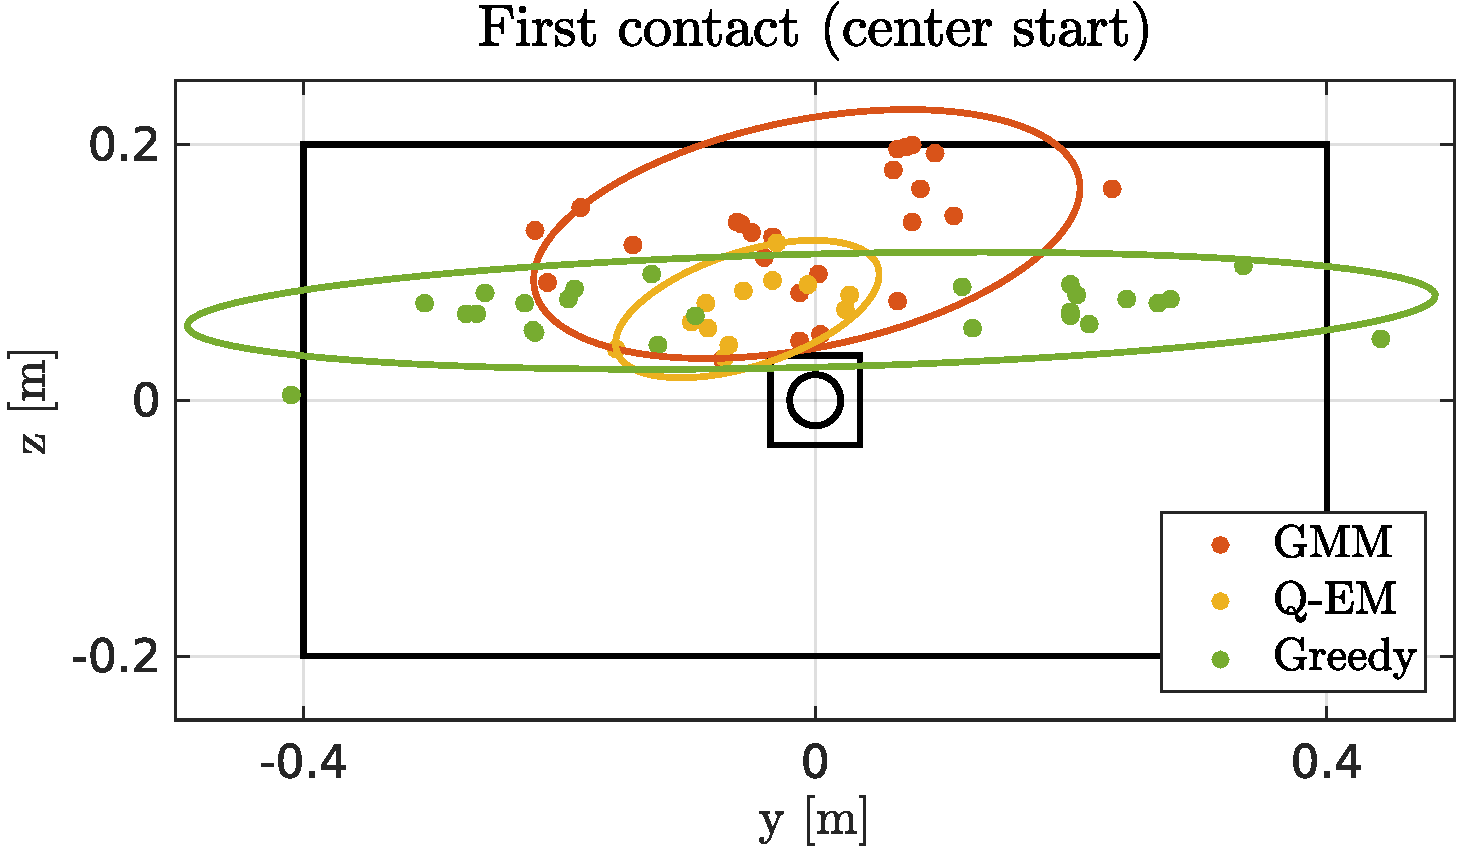
\includegraphics[width=0.45\textwidth]{./ch4-PiH/Figures/Fig/first_contact_center.pdf}
   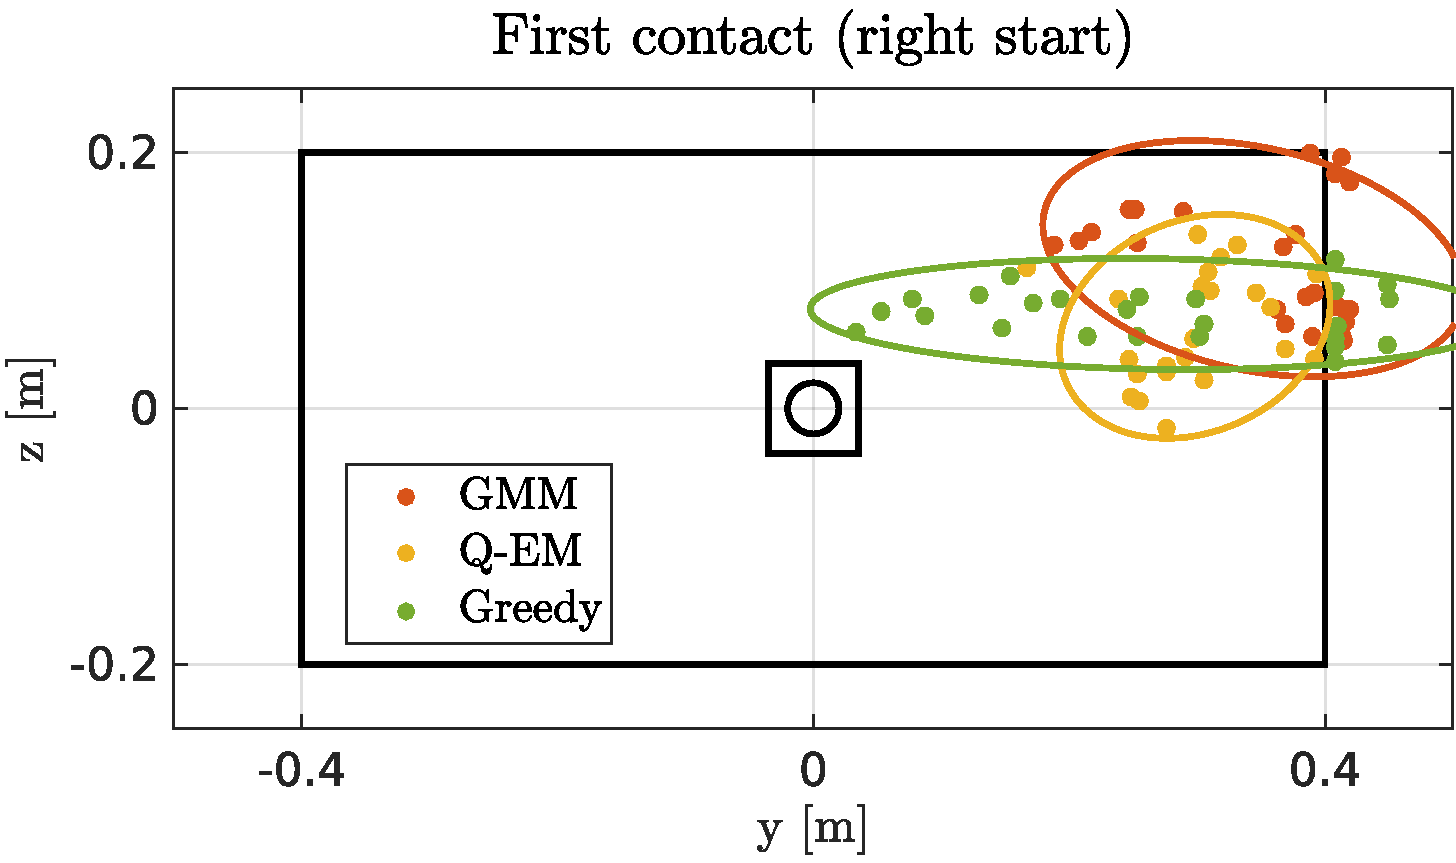
\includegraphics[width=0.45\textwidth]{./ch4-PiH/Figures/Fig/first_contact_right.pdf}
   \caption{First contact with the wall, during experiment 1. (a) Contact distribution for initial condition ``Center'' . (b) 
   Contact distribution for initial condition was ``Right''. The ellipses correspond to two standard deviations of a fitted Gaussian 
   function.}
   \label{fig:first_contact}
\end{figure}

\subsection{Distance taken to reach the socket's edge (Quantitative)}

In Figure \ref{fig:three_searches} we illustrate the quantitative results of the distance taken 
to reach the socket for all three experiments. In \textbf{Experiment 1}, for the \textit{Center} initial condition,
the Q-EM policy travels far less than the other search policies. Considering that the initial position of the search is 
0.45 [m] away from the wall, the Q-EM policy finds the socket very quickly once contact has been established with the wall. 
For the \textit{Right} and \textit{Left} starting conditions both the GMM and Q-EM policies travel less distance to reach the socket, with a 
smaller variance when compared with the Greedy search policy.

In \textbf{Experiment 2}, Figure \ref{fig:three_searches}, the Q-EM search policy is the most efficient. For \textit{Case 1} 
of Experiment 2, the initial most likely state is fixed to the left and the true position is facing the socket. 
As the belief is chosen to be to the left, upon contact with the wall the policy takes a left action since it 
is more likely to result in a localisation. 
On average this results in an exploration of the upper left area of the wall, which explains why \textit{Case 1} of Experiment 2 
performs worse than Experiment 1 for the \textit{Center} initial condition. In \textit{Case 2} however, where the 
true state is facing the left edge and the believed position is facing the right edge, less distance is taken to find the 
socket than for \textit{Case 1}, Figure \ref{fig:three_searches} (b). This improvement over \textit{Case 1} is due to the true location of 
the end-effector being closer to an informative feature and results in a much faster localisation.

From \textbf{Experiment 3}, Figure \ref{fig:three_searches_exp3}, it is clear that all three search policies travel 
less to find the socket's edge compared with the teachers' demonstrations. 
All search policies are better than the human teachers with the exception of group B\textsuperscript{*}, 
which is performing the task with socket A. The Q-EM policy remains the best. 

\begin{figure}
 \centering
  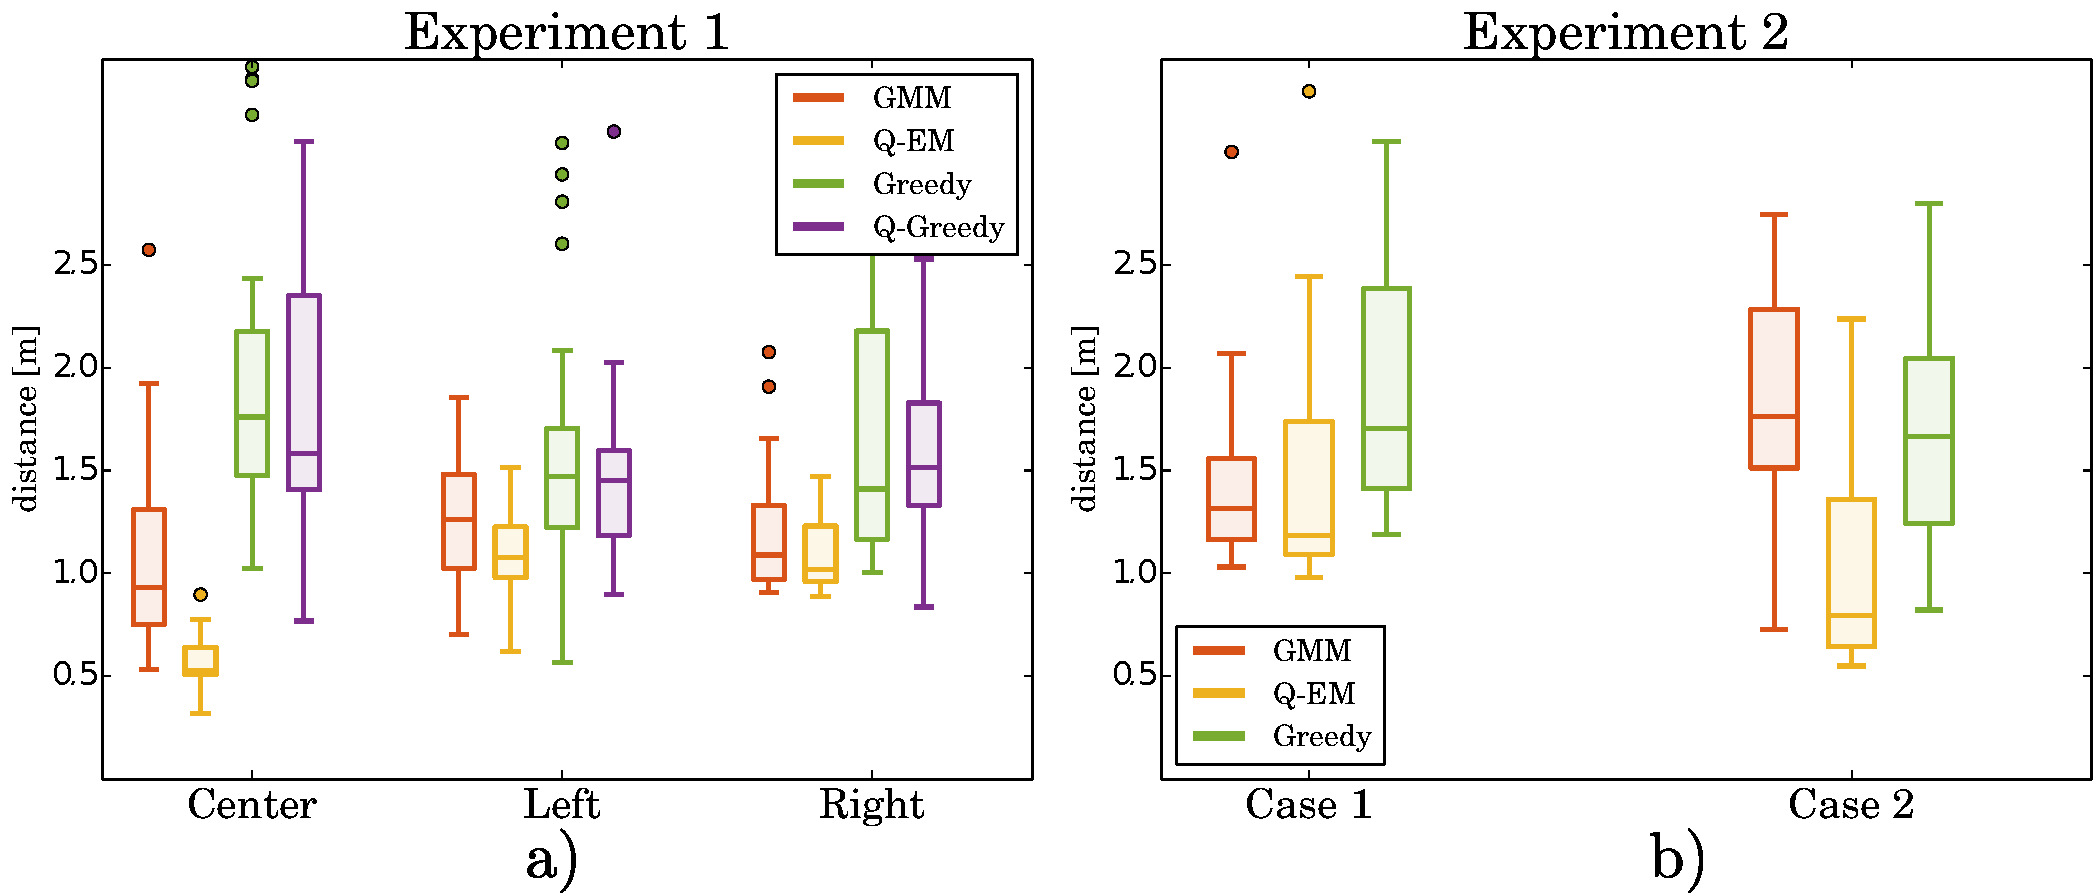
\includegraphics[width=\textwidth]{./ch4-PiH/Figures/Fig/experiment_1_2.pdf}
  \caption{Distance travelled until the socket's edge is reached. a) Three groups correspond to the initial conditions: Center, Left and Right
   depicted in Figure \ref{fig:box_exp_sim}, \textit{top left}. The Q-EM method is always better than the other methods, in terms of distance. b)
   Results of the two initial conditions depicted in Figure \ref{fig:box_exp_sim}, \textit{top middle}, both the true position and most likely state are
   fixed. The Q-EM method always improves on the GMM. }
   \label{fig:three_searches}
\end{figure}
\begin{figure}
 \centering
  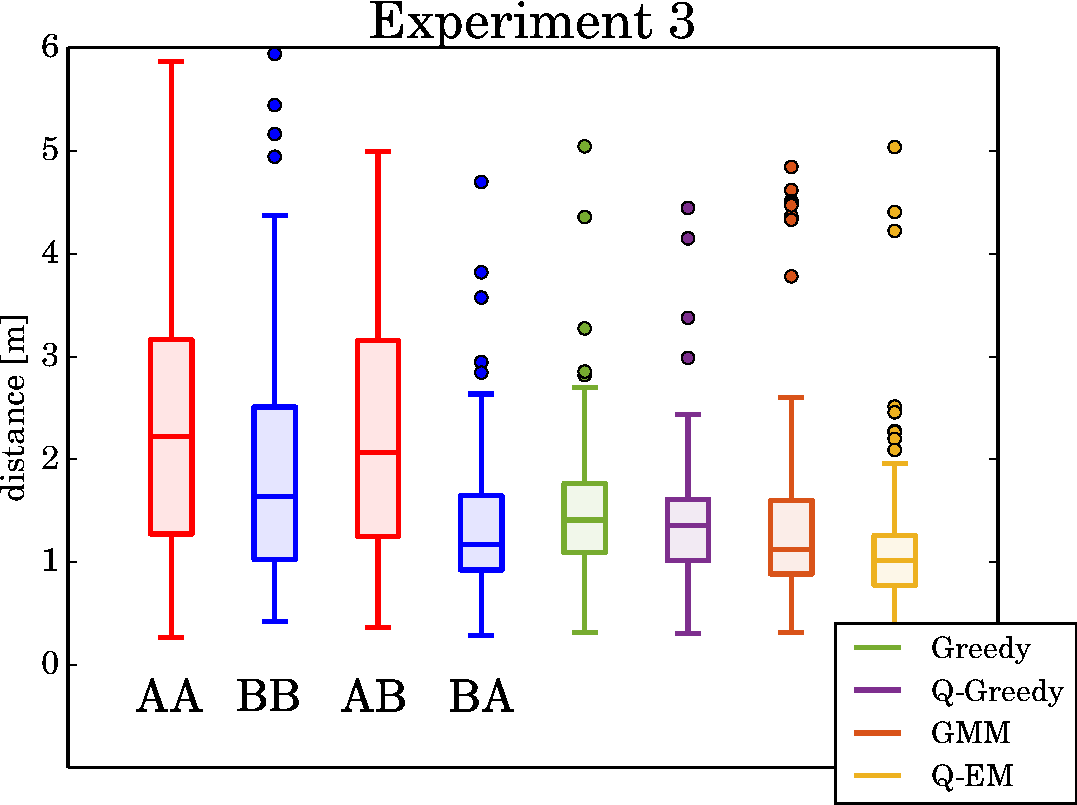
\includegraphics[width=0.6\textwidth]{./ch4-PiH/Figures/Fig/experiment3_plot2.pdf}
  \caption{Distance travelled until the socket's edge is reached. Results corresponding to Experiment 3, Figure \ref{fig:box_exp_sim}, \textit{top right}.
   Again the Q-EM method is better, but at a less significant level.}
   \label{fig:three_searches_exp3}
\end{figure}
 

We have shown that under three different experimental settings the Q-EM algorithm is predominantly the best in terms of distance taken 
to localise the socket. The GMM policy learned solely from the data provided by the human teachers also performs well in comparison to  
the human teachers and Greedy policy. We made, however a critical assumption in order to be able to use our (RL-)PbD-POMDP approach. 
This \textbf{assumption} is that a human teacher is proficient in accomplishing the task. If a teacher is not able to accomplish 
the task in a repetitive and consistent way so that a search patter can be encoded by the GMM, the learned policy will perform poorly.
Next we evaluate the validity of this assumption and the importance of the training data provided by the human teachers.
% 
\subsection{Importance of data}

We perform two tests to evaluate the importance of the teachers training data for learning a search policy. Firstly we take the 
worst two teachers in terms of distance taken to find the socket's edge and learn a GMM and Q-EM policy separately from their 
demonstrations. In this way we can evaluate whether it is possible to learn a successful policy given 
a few bad demonstrations (15 training trajectories for each policy). Our second evaluation consists of using a noisy 
explorative Greedy policy as a teacher to gather demonstrations which can then be used to learn a new policy, which we call Q-Greedy. 

Figure \ref{fig:subj_5_traj} illustrates 6 trajectories of teacher \# 5. The human teacher preferred to
localise himself at the top of the wall before either proceeding to a corner or going directly towards the socket. Once localised, the teacher 
would reposition himself in front of the socket and try to achieve an insertion. This behaviour was not expected 
since by losing contact with the wall, the human teacher no longer had sensory feedback necessary 
to maintain an accurate position estimate.

\begin{figure}
 \centering
    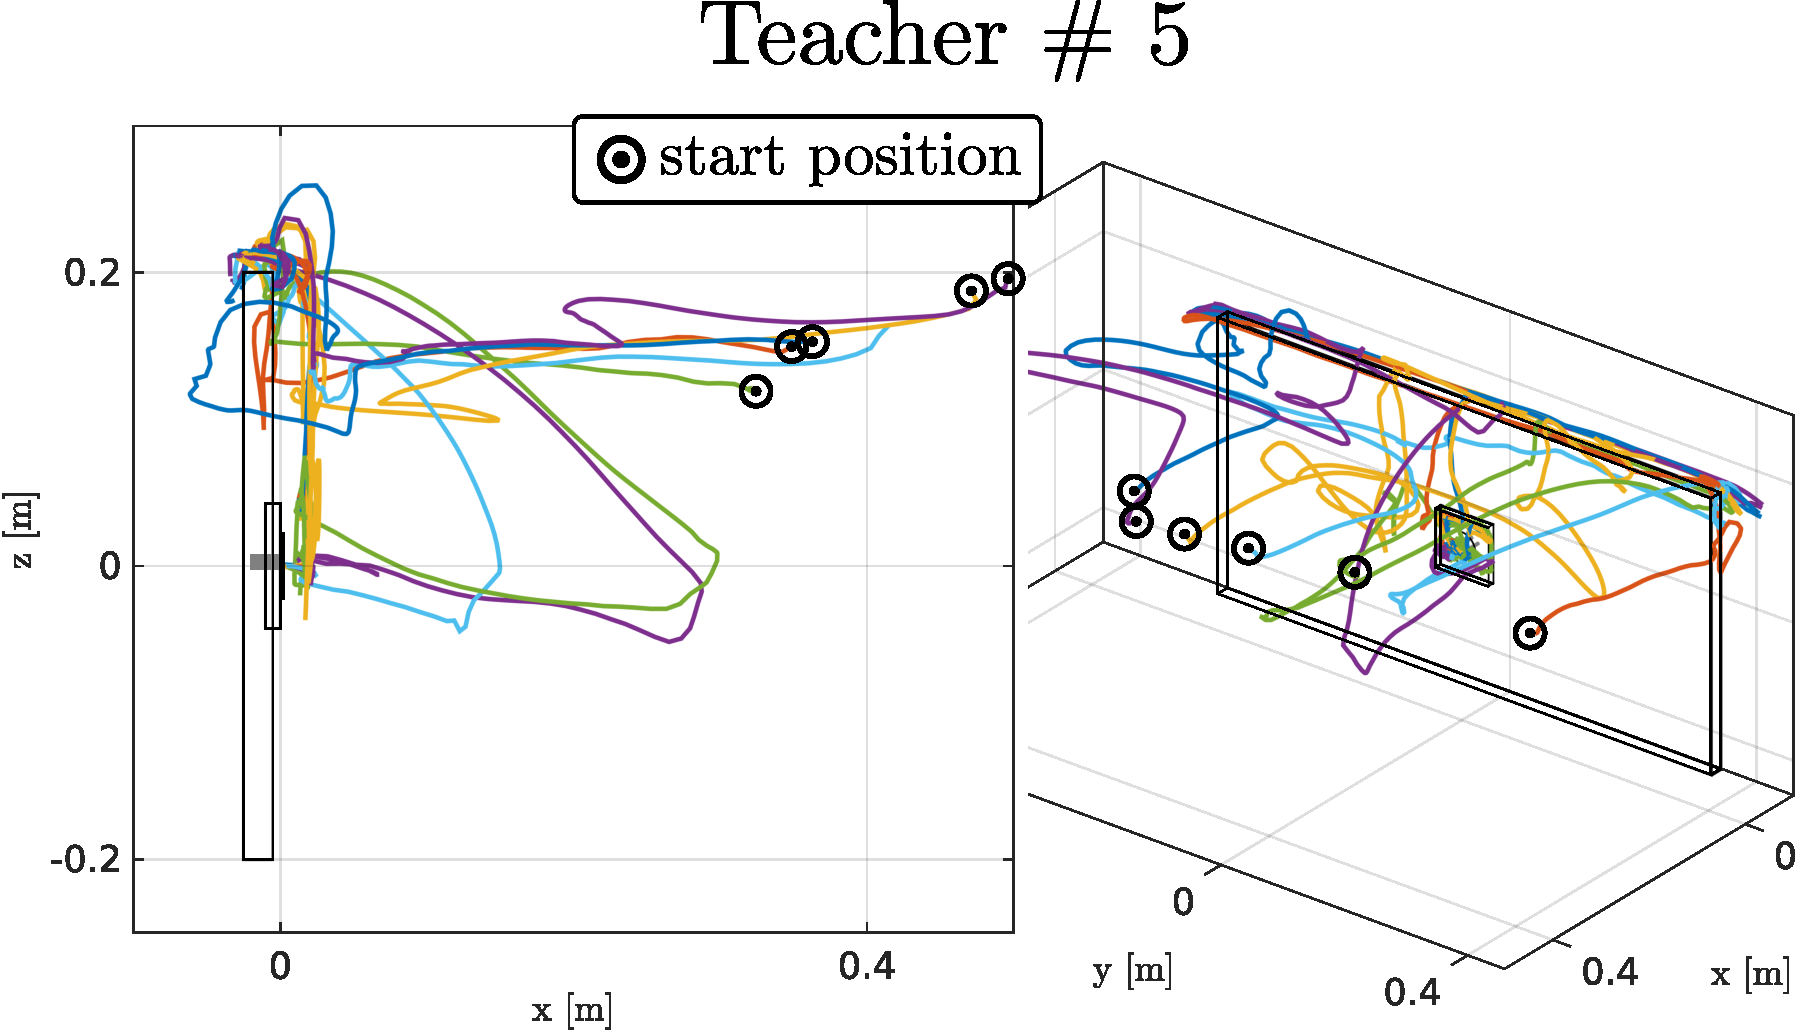
\includegraphics[width=\textwidth]{./ch4-PiH/Figures/Fig/subject5.pdf}
%    \subfigure[]{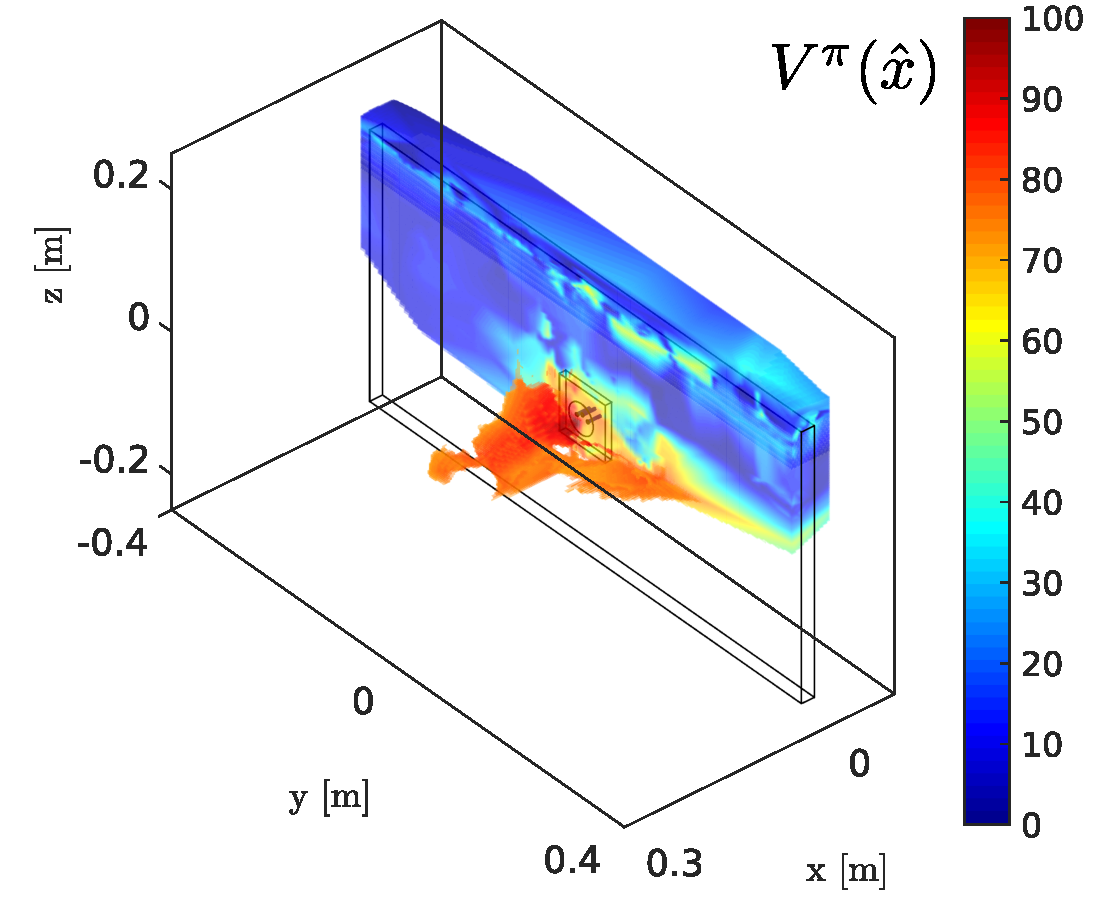
\includegraphics[width=0.45\textwidth]{./Figures/Results1/experiment4/value_subj_5.pdf}}
%    \subfigure[]{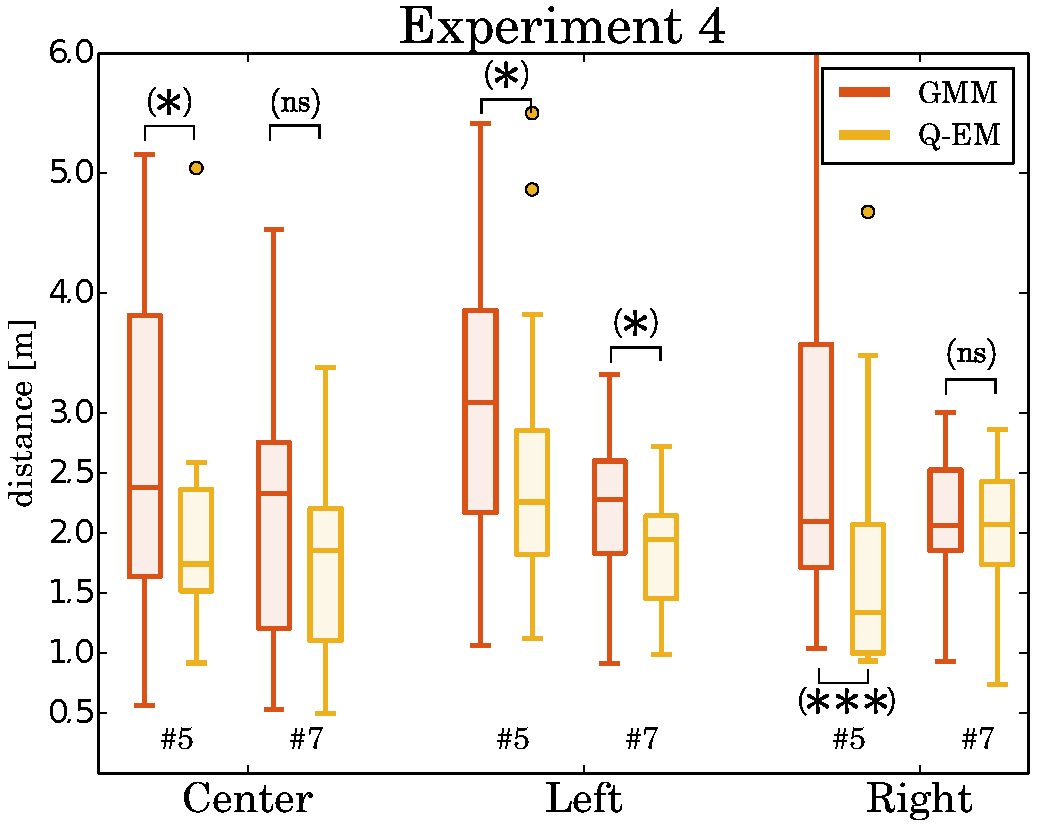
\includegraphics[width=0.445\textwidth]{./Figures/Results1/experiment4/experiment4.pdf}}
    \caption{Demonstrations of teacher \# 5. The teacher demonstrates a preference}
    \label{fig:subj_5_traj}
 \end{figure}
 
\begin{figure}
 \centering
 \includegraphics[width=0.8\textwidth]{./ch4-PiH/Figures/Fig/value_subj_5.pdf}
 \caption{Value function learned from the 15 demonstrations of teacher \#5. The value of the the most likely state is plotted.}
 \label{fig:value_function_subj_5}
\end{figure}
 
 \begin{figure}
    \centering
    \includegraphics[width=\textwidth]{./ch4-PiH/Figures/Fig/gmm_v2c.pdf}
    \caption{Marginalised Gaussian Mixture parameters of the GMM and Q-EM learned from the demonstrations of teacher \#5. 
    The illustrated transparency of the Gaussian functions is proportional to their weight.
    \textit{Left column}: The Gaussian functions of the Q-EM have shifted from the left corner to the right. This is a result of the value function 
    being higher in the top right corner region, see Figure \ref{fig:value_function_subj_5}. \textit{Center column}:  The original data of the teacher 
    went quite far back which results in a Gaussian function given a direction which moves away from the wall (green arrow), whilst in the case
    of the Q-EM parameters this effect is reduced and moved closer towards the wall.  We can also see from the two plots of the Q-EM parameters 
    that they then follow the paths encoded by the value function.    
    \textit{Right column}: Rollouts of the policies learned from teacher \#5. We can see that trajectories from the GMM policy have not really 
    encoded a specific search patter, whilst the Q-EM policy gives many more consistent trajectories which replicate to some extent 
    the pattern of making a jump (no contact with the wall) from the top right corner to the socket's edge.}
    \label{fig:gmm_exp4}
\end{figure}
 
Figure \ref{fig:value_function_subj_5} illustrates the value function of the belief state learned from the data of teacher \# 5.
The states with the highest values seem to create a path going from the socket towards the right edge of the wall. 
We proceed as before to learn a GMM policy from the raw data and a Q-EM policy in which the data points are weighted by 
the gradient of the value function. In Figure \ref{fig:gmm_exp4}, we illustrate the 
resulting Marginalised Gaussian Mixture parameters for both the GMM and Q-EM policies and we plot 25 rollouts of each policy starting at 
the \textit{Center} initial condition used in Experiment 1. We note that the trajectories of the GMM 
policy have much variance in contrast to the Q-EM policy, resulting from an excess of variance in the 15 original demonstrations
given by the teacher. Too much variance is not necessarily good, a random (uniform) policy in terms of generated trajectories
will have the most variance and is as expected extremely inefficient in achieving a goal. Furthermore there is insufficient data to encode a pattern for the GMM model. In contrast, the Q-EM finds a 
pattern by combining multiple parts of the available data and as a result fewer data points are necessary to achieve a good policy. 
This effect is clear in Figure \ref{fig:experiment4_stats}, showing the performance of the GMM and Q-EM algorithms 
under the same initial conditions as in Experiment 1. For all the conditions and for both teachers \#5 and \#7 the Q-EM policy 
always does better than the GMM.

\begin{figure}
 \centering
 \includegraphics[width=0.8\textwidth]{./ch4-PiH/Figures/Fig/experiment4.pdf}
 \caption{Results of a GMM and Q-EM policy under the same test conditions as Experiment 1. The Q-EM policy nearly always does much better than the GMM policy.}
 \label{fig:experiment4_stats}
\end{figure}

We also tested whether we could use the Greedy policy as a means of gathering demonstrations in order to learn a value function and 
train a Q-Greedy policy. We used the Q-Greedy algorithm in combination with random perturbations applied to the Greedy velocity, to act as 
a simple exploration technique. We performed a maximum of 150 searches, which terminated once the socket was found and used these demonstrations to 
learn a value function and GMM policy which we refer to as Q-Greedy. Figure \ref{fig:three_searches} illustrates the statistical results 
of the Q-Greedy policy for Experiment 1 and 3, showing that there is no difference between two policies. 
Our exploration method is probably too simplistic to discover meaningful search patterns and we could probably devise better 
search strategies which would result in a good policy. However we have shown that human behaviour does already have a usable trade-off 
between exploration and exploitation which can be used to learn a new policy through our RL-PbD-POMDP framework.

\subsection{Generalisation}

An important aspect of a policy or any machine learning methodology is to be able to generalise. So far we have trained and 
evaluated our policy within the same environment. To test whether our GMM policies can generalise to a new setting we changed 
the location of the socket to the upper right corner of the wall. The GMM was trained in the frame of reference of the socket and
when we translated the socket's location it also translated the policy. 

\begin{figure}
 \centering
    \subfigure[]{\includegraphics[width=\textwidth]{./ch4-PiH/Figures/Fig/traj_experiment5.pdf}}
    \caption{Evaluation of generalisation. The socket is located in at the top right corner of the wall. We consider a 
    \textit{Fixed} starting location for both the true and believed location of the end-effector. The red square depicts the 
    extent of the initial uncertainty, which is uniform. (b) Distance taken to reach the socket's edge. For the Fixed setup (see (a) for 
    the initial condition), both the Q-EM and GMM significantly outperform the Greedy. The other three conditions are the same as for 
    Experiment 1. }
    \label{fig:experiment5_traj}
\end{figure}

\begin{figure}
 \centering
    \subfigure[]{\includegraphics[width=0.8\textwidth]{./ch4-PiH/Figures/Fig/experiment5.pdf}}
    \caption{Distance taken to reach the socket's edge. For the Fixed setup (see Figure \ref{fig:experiment5_traj}) for 
    the initial condition), both the Q-EM and GMM significantly outperform the Greedy. }
    \label{fig:experiment5_stats}
\end{figure}

To evaluate the generalisation of our learned policy we use the same initial conditions of Experiment 1 with an additional 
new configuration named \textit{Fixed}, in which both the true and believed location are fixed, blue triangle and circle.
Figure \ref{fig:experiment5_traj} illustrates the trajectories of the three search policies for the \textit{Fixed} initial condition. 
The Greedy policy moves in a straight line towards the top
right corner of the table. As the true position is to the right, it takes the Greedy policy longer to find the wall 
in contrast to both the GMM and Q-EM policies. From the statistical results shown in Figure \ref{fig:experiment5_stats} we can see
that for the \textit{Fixed} and \textit{Right} initial condition, which are similar, both GMM and Q-EM are better. However, for 
the \textit{Center} and \textit{Left} initial condition this is no longer the case. 
The Greedy method is better under this condition since the socket is close to informative features (it is located close to the edges of the wall). 
Once the end-effector has entered in contact with the wall the actions of the Greedy policy always result in a decrease of uncertainty, which was not the case when the socket was located in the center of wall. 
Thus in both the \textit{Fixed} and \textit{Right} initial condition the Greedy method does worse because it takes longer
to find the wall.

The GMM based policies are still able to generalise under different socket locations. In general, as the socket's location is moved 
further from the original frame of reference in which it was learned, the higher is the likelihood that the search quality degrades. We 
chose the upper right corner since it is the furthest point from the origin and the GMM and Q-EM policies were still able to find 
the socket. We note that the policy will always be able to find the socket once it has localised itself. This can be seen from the vector field 
of the GMM policy when the uncertainty is low, see Figure \ref{fig:policy_vf} on page \pageref{fig:policy_vf}. In this case the policy is a sink function 
with a single point attractor.

\subsection{Distance taken to connect the plug to the socket}
% Real socket experiment.
% Show initial condition setup with belief. (the experiment)
In this section we evaluate the distance taken for the policies and humans to establish a connection, after the socket 
has been found. We start measuring the distance 
from the point that the plug enters in contact with the socket's edge until the plug is connected to the socket. All the following evaluations are done 
on a KUKA LWR4 robot. The robot's end-effector is equipped with a plug holder on which is attached a force-torque sensor, 
the same holders used during the demonstration of the human teachers. In this way both the teacher and robot apprentice share 
the same sensory interface.

We chose to have the robot's end-effector located to the right of the socket and a belief spread uniformly 
along the z-axis. See Figure \ref{fig:real_pictures} for an illustration of the initial starting condition.
This initial configuration was used to evaluate the search policies for the three different sockets, see Figure \ref{fig:search_task_setup} 
on page \pageref{fig:search_task_setup} for an illustration of the sockets. The same initial configuration for 
the evaluation of the three sockets was kept in order to observe the generalisation properties of the policies. 
As a reminder we used only the training data from demonstrations acquired during the search with socket A. Socket B has a funnel which should make it 
easier to connect whilst socket C should be more difficult as it has no informative features on its surface. 

For each of the sockets we performed 25 searches starting from the same initial condition. In Figure \ref{fig:real_policy} we plot
the trajectories of each of the search methods for socket A. The GMM reproduces some of the behaviour exhibited by humans, such as 
first localising itself at the top of the socket before trying to attempt to make a connection. The Q-EM algorithm exhibits less variation
than the GMM and tends to pass via the bottom of the socket to establish a connection. The Greedy method in contrast is much more  
stochastic since it does not take into consideration the variance of the uncertainty but tries instead to directly establish a connection.
Figure \ref{fig:real_statistics} (c) shows that for socket A both the Greedy and Q-EM are better than the GMM and the Q-EM has less
variance in comparison to the Greedy searches.  All three search methods are vastly superior, when compared to the human's performance 
see Figure \ref{fig:real_statistics}.  In Figure \ref{fig:real_pictures} illustrates a typical rollout of the GMM search policy for both 
socket A and C. Once a contact is made with the socket's edge the policy tends to stay close to informative features and tends to 
wander vertically up and down. Only when the uncertainty has been reduced does the GMM policy try to go towards the socket's connector. 

\begin{figure}
 \centering
    \subfigure[]{\includegraphics[width=\textwidth]{./ch4-PiH/Figures/Results2/socket_connection_A.pdf}}
    \caption{%(a) All three sockets have the same connector interface, but have different structures. Both 
   % socket A and B have an edge around the center whilst the surface of socket C is featureless and more elevated than the other two. 
    25 search trajectories for each of the three search policies for socket A. }
    \label{fig:real_policy}
\end{figure}


\begin{figure*}
 \centering
 \subfigure[]{\includegraphics[width=0.95\textwidth]{./ch4-PiH/Figures/Results2/s1_sequence.pdf}}
 \subfigure[]{\includegraphics[width=0.95\textwidth]{./ch4-PiH/Figures/Results2/s2_sequence.pdf}}
 \caption{KUKA LWR4 equipped with a holder mounted with a ATI 6-axis force-torque sensor. (a) The robot's end-effector starts to the 
 right of socket A. The second row shows screen captures taken of ROS Rviz data visualiser in which we see the Point Mass Filter 
 (red particles) and a yellow arrow indicating the direction given by the policy. In this particular run, the plug remained in contact with the ring of the socket until 
 the top was reached before making a connection. (b) Same initial condition as in (a) but with socket C. The policy leads the plug down to 
 the bottom corner of the socket before going the center of the top edge, localising itself, and then making a connection.}
 \label{fig:real_pictures}
\end{figure*}

\begin{figure}
 \centering
   \includegraphics[width=\textwidth]{./ch4-PiH/Figures/Results2/real_exp_socketAB.pdf}
  % \subfigure[]{\includegraphics[width=0.3\textwidth]{./ch4-PiH/Figures/Results2/real_exp_socketB.pdf}}
  % \subfigure[]{\includegraphics[width=0.3\textwidth]{./ch4-PiH/Figures/Results2/peg_socket_connection.pdf}}
  \caption{Distance taken to connect plug to socket once the socket is localised. (a) \textbf{Socket A}. The human 
  Group A are the set of teachers who first started with socket A. They had no previous training on another socket beforehand. Group 
  B\textsuperscript{*} first gave demonstrations on Socket B before giving demonstrations on Socket A. Group B\textsuperscript{*}
  is better than Group A at doing the task. This is most likely a training effect. However all policy search methods are far better
  at connecting the plug to the socket. (b) \textbf{Socket B}. Both Groups A\textsuperscript{*} and B are similar in terms 
  of the distance they took to insert the plug into the socket and as was the case for (a), the search policies travel less to accomplish 
  the task.   } 
  \label{fig:real_statistics}
\end{figure}

\begin{figure}
 \centering
   \includegraphics[width=0.8\textwidth]{./ch4-PiH/Figures/Results2/peg_socket_connection_v2.pdf}
   \caption{Distance taken (measured from point of contact of plug with socket edge) to connect the plug to the socket.}
  \label{fig:real_statistics2}
\end{figure}

The GMM and Q-EM policies are able to generalise to both socket B and C, as the geometric shape and connector interface of the 
two sockets are similar to socket A. The local force modulation of the policy's vector field, which is not learned, allows the 
end-effector to surmount edges and obstacles whilst trying to maintain a constant contact force in the x-axis. This modulation makes it possible for the plug to get on top of socket C.
Figure \ref{fig:real_statistics} (c) illustrates the statistics of the distance taken to establish a connection for all three sockets. 
The interesting point is that both the GMM and Q-EM algorithms perform better than the Greedy approach for socket C. Socket C has no informative 
features on its surface and as a result myopic policies such as the Greedy policy will perform poorly. However for socket A 
and B, the Greedy policy performs better as both of these sockets have edges around their connector point allowing for easy localisation. 
It can also be seen that most search methods perform better on socket B than A, since the funnel shape connector helps in maintaining the plug 
within the vicinity of the socket's holes. 


The discrepancy between the humans performance and the search policies can be attributed to many causes. One plausible reason is 
that the PMF probability density representation of the belief is more accurate than the human teachers position belief. 
Also, the motion noise parameter was fixed to be proportional to the velocity and the robot moves at gentle pace ($\sim1$ cm/s) as 
opposed to some of the human teachers. In actuality, humans are far less precise than the KUKA which has sub-millimetre accuracy.

\section{Discussion \& Conclusion}\label{ch4:conclusion}
% Recapulate what we did 
%
% We learned a 
%
%

In this work we learned search policies from demonstrations provided by human teachers for a task
which consisted of first localising a power socket (either socket A, B or C) and then connecting it with a plug. Only haptic information 
was available as the teachers were blindfolded. We made the assumption that the position belief of the human teachers 
was initially uniformly distributed in a fixed rectangular region of which they were 
informed and is considered prior knowledge. All subsequent beliefs were then updated in a Bayesian recursion 
using the measured velocity obtained from a vision tracking system, and wrench acquired from a force torque sensor attached 
to the plug. The filtered probability density function, represented by a Point Mass Filter, was then compressed to the 
most likely state and entropy.

Two Gaussian Mixture Model policies were learned from the data recorded during the human teachers' demonstrations. 
The first policy, called Q-EM, was learned in an Actor-Critic RL framework in which a value function was learned over 
the belief space. This was then used to weight training datapoints in the M-step update of Expectation-Maximisation (EM). The second 
policy, called GMM, was learned using the standard EM algorithm, and considered all training data points equally,
following in the footsteps of our initial approach \cite{Chambrier2014}. Both the Q-EM and GMM policies were trained 
with data solely from the demonstrations of the search with socket A.

We evaluated 4 different aspects of the learned policies. Firstly, we evaluated which of three policies, Q-EM, GMM and a Greedy policy, 
took the least distance to find the socket. We concluded that across three different Experiments the Q-EM algorithm always performed
the best. It was clear that the Q-EM policy was less random and more consistent than the GMM policy as it tried to enter in 
contact with the wall at the same height as the socket thus increasing the chances of finding the socket.

Secondly, we tested the importance of the data provided by the human teachers. We took the worst two teachers and trained an
individual GMM and Q-EM policy for each of them. We found that the performance of the Q-EM was better than the GMM in terms 
of distance travelled to find the socket. When qualitatively evaluating the trajectories of the GMM with respect to the 
Q-EM for the worst teacher, it is clear that the Q-EM policy managed to extract a search pattern, which was not the case 
for the GMM policy. We also tried to learn a Q-EM policy from the data provided by a Greedy policy with explorative noise 
and we found no improvement. From these results we conclude that the exploration and exploitation aspects of the trajectories 
provided by the human teachers is necessary.

Thirdly, we tested whether the two policies (GMM and Q-EM) were able to generalise to a different socket location. Under a specific condition,
which we called \textit{Fixed}, both policies were significantly better than the Greedy policy. However for the \textit{Center}
and \textit{Left} initial conditions the Greedy policy performed better. For the initial conditions in which the Greedy policy 
enters in contact with the wall at an early stage, it also performs better than the GMM and Q-EM. The reason for this is that  
the actions taken by the Greedy policy in this setting will always result in a decrease of entropy when the location
of the socket is close to a corner, as opposed to being in the center of the wall.

Fourthly, we evaluated all three policies on the KUKA LWR4 robot and found that all the policies did better than the human 
teachers. For socket A, on which both the GMM and Q-EM policies were trained, there is no clear distinction between 
the Q-EM and Greedy policy. On socket B, which was novel, the Greedy policy performed better than the statistical controllers, 
which we hypothesize was a result of a funnel which would make it easier for a myopic policy. For socket C, both the 
GMM and Q-EM policies performed better than the Greedy, as socket C has no features on its surface, this being a disadvantage 
for a myopic policy.

We conclude by making the observation that by simply adding a binary reward function in combination with 
data provided by human demonstrations, with Fitted reinforcement learning, we can learn a better policy without 
the need to perform expensive exploration-exploitation rollouts traditionally associated with reinforcement learning and 
designing complicated reward functions. This is especially advantageous when only a few demonstrations are available.

\FloatBarrier
\section{Appendix}

\subsection{Time to connect socket (ANOVA)}
\label{app:anova_socket}
% 1) Is there are a difference across groups 

% 2) Is there a difference between the two sockets
The null hypothesis is that there is no difference in 
the time taken to connect socket A or B. The result of the one-way anova
is given in Table \ref{tab:ch4:anova_socket}. The null hypothesis is rejected at high significant level (***)
indicating that there is a difference between the sockets. According to the linear 
model it takes on average 4 seconds less to connect socket B than it does for socket A.

\begin{table}[h]
\centering
\begin{tabular}{lcc}
  \hline
          &   F    & Pr(>F)  	     \\ \hline
   socket & 13.9   &  0.000232 *** 
\end{tabular}
\caption{One way anova of the time taken to connect two sockets A and B. There is a significant difference.}
\label{tab:ch4:anova_socket}
\end{table}

We tested whether the group order had an effect on the connection time. We fitted a linear model
with the predictor being time and the factors being the group (One or Two), the socket type (A or B) 
and the subject's ID (1 to 10):
\begin{equation}
 time = \beta_0 + \beta_1\, group + \beta_2\, socket + \beta_3\, subject
\end{equation}
and did the corresponding anova analysis on this linear model. We found that the difference between the sockets 
remained significant.

\subsection{EM policy search}\label{app:lb}
Steps taken to make a policy $\pi_{\Param}(\U,\B)$ maximise the objective function, $J(\Param)$.
The policy will be maximised with respect to the lower bound of the cost function $J(\Param)$:
\begin{align}
  J(\Param') &= \sum_{i \in \mathbb{T}} \pi_{\Param'}(\Ui,\Bi)\, R(\Ui,\Bi) \nonumber\\ 
	   &= \sum_{i \in \mathbb{T}}  \frac{\pi_{\Param'}(\Ui,\Bi)}{\pi_{\Param}(\Ui,\Bi)} \, \pi_{\Param}(\Ui,\Bi) \, R(\Ui,\Bi)
\end{align}

where $\mathbb{T}$ is the set of all rollouts. Next we take the logarithm and make use of Jensen's inequality and move the logarithm into the 
summation.

\begin{align}
  \log( J(\Param') )  &= \log \sum_{i \in \mathbb{T}} \frac{\pi_{\Param'}(\Ui,\Bi)}{\pi_{\Param}(\Ui,\Bi)} \, \pi_{\Param}(\Ui,\Bi) \, R(\Ui,\Bi) \nonumber \\
		     & \geq \sum_{i \in \mathbb{T}}\log\Bigg( \frac{\pi_{\Param'}(\Ui,\Bi)}{\pi_{\Param}(\Ui,\Bi)}\Bigg) \, \pi_{\Param}(\Ui,\Bi) \, R(\Ui,\Bi) \label{eq:lower_bound}
\end{align}

We take the derivative of the lower bound of $\log(J(\Param'))$, Equation \ref{eq:lower_bound}, with respect to $\Param'$ and set it to 
zero so as to maximise the cost function.

\begin{align}
 &\nabla_{\Param'}  \log( J(\Param') ) = \nonumber\\
 &\sum_{i \in \mathbb{T}} \nabla_{\Param'} \log\big( \pi_{\Param'}(\Ui,\Bi)\big) \, \pi_{\Param}(\Ui,\Bi) \, R(\Ui,\Bi) \nonumber \\
				    & - \underbrace{ \nabla_{\Param'} \log\big( \pi_{\Param}(\Ui,\Bi)\big) \, \pi_{\Param}(\Ui,\Bi) \, R(\Ui,\Bi)}_{\color{red} =0} \nonumber \\
				    &= \sum_{i \in \mathbb{T}} \nabla_{\Param'} \log\big( \pi_{\Param'}(\Ui,\Bi)\big) \, \pi_{\Param}(\Ui,\Bi) \, R(\Ui,\Bi) \nonumber \\
				    &= \mathbb{E}_{\pi_{\Param}(\U,\B)} \Big\{ \nabla_{\Param'} \log\big( \pi_{\Param'}(\Ui,\Bi)\big)\, R(\Ui,\Bi) \Big\}
\end{align}

\begin{align}
 \nabla_{\Param'}  \log( J(\Param') ) &= \mathbb{E}_{\pi_{\Param}(\U,\B)}\Big\{R(\Bi,\Ui)  \sum_{t=0}^{T}\nabla_{\Param'}\log \pi_{\Param'}(\Ui,\Bi)\Big\}\\
				    &= \sum\limits_{i=1}^{N} \sum\limits_{t=0}^{T^{[i]}} \nabla_{\Param'}\log \pi_{\Param'}(\U^{[i]}_t,\B^{[i]}_t) \, Q^{\pi}(\U^{[i]}_t,\B^{[i]}_t) \label{eq:grad_log_cost_2}
\end{align}

The reader is referred to \cite{rl_gradient_survey_2013} for more details regarding Expectation-Maximisation and policy search in reinforcement learning.

\subsection{Q-EM for GMM derivation}\label{app:grad}

Making the substitution $\X = (\U,\B)^{\mathrm{T}}$ (small abuse of the notation) and  insuring a positive Q-function, $Q^{\pi}(\X^{[m]}) \geq 0$
and by setting the derivative of Equation \ref{eq:grad_log_cost_2} to zero and solving for the parameters
$\Param=\{w,\boldsymbol{\mu},\boldsymbol{\Sigma}\}$ we get a new weighted Maximisation update step in EM:

\begin{align}
\nabla_{\MuK} \log J(\Param) =& \sum\limits_{m=1}^{M} \alpha(z_{mk})\, Q(\Xm)\, \invSigK (\Xm - \MuK) = 0 \nonumber \\
			 \MuK_{\textrm{\textbf{new}}} =& \frac{\sum\limits_{m=1}^{M} \alpha(z_{mk})\, Q(\Xm)\, \Xm }{\sum\limits_{j=1}^{M} \alpha(z_{jk})\, Q(\X^{[j]})}
\end{align}

where $\alpha(z_{mk})$ is the responsibility factor, denoting the probability that data point $m$ is a member of the 
Gaussian function $k$.

\begin{equation}
 \alpha(z_{mk}) = \frac{w^{[k]} \cdot g(\Xm;\MuK,\SigK)}{\sum\limits_{j=1}^{K}w^{[j]} \cdot g(\Xm;\boldsymbol{\mu}^{[j]},\boldsymbol{\Sigma}^{[j]})}
\end{equation}

\begin{equation}
   \SigK_{\textrm{\textbf{new}}} = \frac{\sum\limits_{m=1}^{M} Q(\Xm) \alpha(z_{mk}) (\Xm - \MuK)(\Xm - \MuK)^{\mathrm{T}} }{ \sum\limits_{j=1}^{M} Q(\X^{[j]})\, \alpha(z_{jk}) }
\end{equation}

\begin{equation}
  w^{[k]}_{\textrm{\textbf{new}}} = \frac{\sum\limits_{m=1}^{M} Q(\X^{[m]})\, \alpha(mk)}{\sum\limits_{j=1}^{M} Q(\X^{[j]})}
\end{equation}

%\subsection{M-step}\label{app:Q-EM}
%Given a set of points $\X = (\U,\B)^{\mathrm{T}}$ and  a positive Q-function, $Q^{\pi}(\X^{[m]}) \geq 0$
%and by setting the derivative of Equation \ref{eq:grad_log_cost} to zero and solving for the parameters
%$\Param=\{w,\boldsymbol{\mu},\boldsymbol{\Sigma}\}$ we get a new weighted Maximisation updates in EM:
%\begin{align}
% w^{[k]}_{\textrm{\textbf{new}}} &= \frac{\sum\limits_{m=1}^{M} Q^{\pi}(\X^{[m]})\, \alpha(z_{mk})}{\sum\limits_{j=1}^{M} Q^{\pi}(\X^{[j]})} \\
% \MuK_{\textrm{\textbf{new}}}     &= \frac{\sum\limits_{m=1}^{M} \alpha(z_{mk})\, Q^{\pi}(\Xm)\, \Xm }{\sum\limits_{j=1}^{M} \alpha(z_{jk})\, Q^{\pi}(\X^{[j]})} \\
% \SigK_{\textrm{\textbf{new}}}    &= \frac{\sum\limits_{m=1}^{M} Q^{\pi}(\Xm)\, \alpha(z_{mk})\, (\Xm - \MuK)(\Xm - \MuK)^{\mathrm{T}} }{ \sum\limits_{j=1}^{M} Q^{\pi}(\X^{[j]})\, \alpha(z_{jk}) }
%\end{align}
%$\alpha(z_{mk})$ is the responsibility factor, denoting the probability that data point $m$ is a member of the 
%Gaussian function $k$ (see \cite[Chap. 9]{Bishop_2006}).

\subsection{Unbiased estimator}\label{app:unbiased_delta}

%\begin{equation}
%  \delta^{\pi}_t = r_{t+1} + \gamma V^{\pi}(b_{t+1}) - V^{\pi}(b_t) \\
%\end{equation}
The temporal difference error is an unbiased estimate of the advantage function:
\begin{align}
  \displaystyle \mathop \mathbb{E}_{\pi_{\Param}} \{ \delta^{\pi}_t|b_t,u_t\} &=  \mathop\mathbb{E}_{\pi_{\Param}}\{ r_{t+1} + \gamma V^{\pi}(b_{t+1})|b_t,u_t\} - V^{\pi}(b_t) \nonumber \\
									   &= Q^{\pi}(b_t,u_t) - V^{\pi}(b_t) \nonumber \\
									   &= A^{\pi}(b_t,u_t)
\end{align}
 	 		\fi
\ifdefined	\gDisplayMLMF	 		\chapter{Non-parametric Bayesian State Space Estimator}

% In this chapter
In both Chapters 3 and 4, we demonstrated that it is feasible to learn a POMDP policy from human teachers. Further,
by adding a simple binary reward function we were able to take into consideration the quality of these demonstrations. 
provided by the teachers. With this, we showed that our Reinforcement Learning extension, RL-PbD-POMDP was able to 
yield improved policies even when provided with a limited number of demonstrations taken from the worst teachers.

Both tasks from the previous two chapters (search for wooden block on a table and peg-in-hole) fall into 
the category of goal oriented \textbf{active-localisation}. In general, the localisation problem consists of estimating 
position parameters given noisy observations whereas active-localisation refers to a policy which actively takes actions to 
acquire information to decrease the uncertainty of the position estimate. In localisation, the model 
of the world also known as the \textbf{map} is considered \textbf{prior knowledge}. This assumption constrains localisation 
to an environment in which schematics exist and can be used 
as the world model such as in the case of offices and buildings. If the map is not known a priori, then Simultaneous Localisation And Mapping (\textbf{SLAM}) algorithms have to be used instead
of localisation. Typically, the map consists of a set of features also known as landmarks which can be identified by sensors, 
and SLAM algorithms maintain a filtered joint probability distribution over both the agent's and features' position which is updated in accordance to a generic 
Bayesian State Space Filter (BSSF) (see Figure \ref{fig:baysian_filter} on page \pageref{fig:baysian_filter}).

In this Chapter, we consider an agent tasked with searching for a set of objects on a \textit{Table} world (see Figure \ref{fig:Figure1}), 
in which exteroceptive feedback is extremely limited. The agent can only sense an object after making physical 
contact with it (bumping into it). The agent's uncertainty of its location and that of the object is encoded by probability distributions $P(\cdot)$, which 
at initialisation are known as the agent's prior beliefs.

Figure \ref{fig:Figure1} illustrates a particular instance of the agent's beliefs. The agent is currently located in the 
bottom  table and has only a limited knowledge of its location, somewhere near the right edge of the table. 

\begin{figure}
  \centering
  \includegraphics[width=0.95\linewidth]{./ch5-MLMF/Figures/Figure1_v2.pdf}
  \caption{ \textit{Table Environment} Table World (delimited by the black rectangle), viewed from above, and the agent's beliefs. 
  There are three different probability density functions present on the table. 
  The blue represents the believed location of the agent, the red and green probability distributions are associated with object 1 and 2.
  The white shapes in each figure represent the true location of each associated object or agent.}
  \label{fig:Figure1}
\end{figure}
\vspace*{0.6cm}

%	2) Current draw back of all SLAM methodologies 
As the agent explores the world, it integrates all sensing information at each time step and updates its prior beliefs to posteriors
(the result of the prior belief after integrating motion and sensory information).
All current SLAM methods are limited in that they only consider uncertainty induced by sensing inaccuracy inherent in 
the sensor and motion models. In our setting as the sensory information is strictly haptic, we can confidently assume no measurement noise. 
In the search task illustrated in Figure \ref{fig:Figure1}, the beliefs and sparse measurement information available to the agent are 
the source of the uncertainty which is, the absence of positive object measurements. 
This is known as \textbf{negative information} \cite[p.313]{Thrun_Burgard_Fox_2005} \cite{Thrun02particlefilters,negative_info_markov_localisation}. 
Thus SLAM methodologies which use the \textbf{Gaussian error} between the predicted and estimated position of features, such as in the case 
of EKF-SLAM and Graph-SLAM, will not work well in this setting. 

{\quote \textit{The EKF SLAM algorithm, [...], can only process positive sightings of landmarks. It cannot process negative information
that arises from the absence of landmarks. } -Probabilistic Robotics \cite[p.313]{Thrun_Burgard_Fox_2005}-}\\[0.01cm]

In addition to the negative sensing information, the original beliefs depicted in Figure \ref{fig:Figure1} are \textbf{non-Gaussian}
and \textbf{multi-modal}. We make \textbf{no assumption} regarding the form the beliefs can take. This implies that the joint distribution 
can no longer be parameterised by a Multivariate Gaussian. 
This is an assumption made in many SLAM algorithms, notably EKF-SLAM, and allows for a closed form solution to the state estimation problem. Without the Gaussian assumption 
no closed form solution to the filtering problem is feasible. 
Using standard non-parametric methods (Kernel Density, Gaussian Process, Histogram,...) to represent or estimate the joint distribution becomes
unrealistic after a few dimensions or additional map features. 
FastSLAM could be a potential candidate, however as it parameterises the position uncertainty of the agent by a particle filter and each
particle has its own copy of the map, the memory demand will become significant.  For planning purposes we would also want to have a 
single representation of the marginals. Figure \ref{fig:ch5_assmuptions} summarises the desirable attributes and assumptions for our filter.

\begin{figure}
\centering
\begin{tikzpicture}    
\node [white_box] (box){%
\begin{minipage}{0.95\textwidth}
\begin{itemize}
  \item Non-Gaussian joint distribution, no assumptions are made with respect to its form.
  \item Mostly negative information available (absence of positive sightings of the landmarks).
  \item Joint distribution volume grows exponentially with respect to the number of objects and states.
  \item Joint distribution volume is dense, there is a lot of uncertainty.
\end{itemize}
\end{minipage}

};
\node[fancytitle, right=10pt] at (box.north west) {Attributes \& Assumptions};
\end{tikzpicture}%
\caption{Assumptions and attributes which have to be fulfilled by our Bayesian State Space Filter. }
 \label{fig:ch5_assmuptions}
\end{figure}

\textit{The main contribution of our work and the importance to the field of Artificial Intelligence} 

An accurate estimate of the agent's belief space is a necessary precondition before planning or reasoning can be carried out.
In a wide range of Artificial Intelligence (AI) applications the agent's beliefs are discrete. This non-parametric representation
is the most unconstraining but comes at a cost. The parameterisation of the belief's joint distribution grows at the rate of a double exponential.
We propose a Bayesian state estimator which delivers the same filtered beliefs as a traditional filter but without explicitly parametrising the 
joint distribution. Through the memorising of the measurement likelihood functions having been applied on the joint distribution 
and by taking advantage of their structure, we achieve a filter which grows linearly as opposed to exponentially 
in both time and space complexity. We refer to our novel filter as the Measurement Likelihood Memory Filter (MLMF) 
it keeps track of the history of measurement likelihood functions, referred to as the memory, which 
have been applied on the joint distribution.
The MLMF filter allows to efficiently process negative information. To the authors knowledge there has been little
research on the integration of negative information in a SLAM setting. Previous work considered the case of active localisation \cite{NegInfoFurtherStudies}.
The incorporation of negative information is useful in many contexts and in particular in Bayesian Theory of Mind \cite{Bake_Saxe_Tene_2011},
where the reasoning process of a human is inferred from a Bayesian Network and in our own work \cite{deChambrier2013} where we model the 
search behaviour of a intentionally blinded human. In such a setting much negative information is present and an efficient belief filter is required. 
Our MLMF is thus applicable to the SLAM \& AI community in general and to the cognitive community which models human or agent behaviours through 
the usage of Bayesian state estimators.

By using this new representation we implement a set of passive search trajectories through the state 
space and demonstrate, for a discretised state space, that our novel filter is optimal with respect to the Bayesian criteria (the successive
filtered posteriors are exact and not an approximation with respect to Bayes rule). We provide an analysis of the space and time complexity of 
our algorithm and prove that it is always more efficient even when considering worst case scenarios.
Lastly we consider an Active-SLAM setting and evaluate the effect of how constraining the size of the number of memorised likelihood 
functions impacts the decision making process of a greedy one-step look-ahead planner.

\section{Outline}

% \hyperref[ch3:background]{\ref{ch3:background}   Background}

The remaining part of this Chapter is structured as follows:


\begin{itemize}
 \item \hyperref[ch5:background]{\ref{ch5:background} Background}: Review of three prominent SLAM algorithms
 and their assumptions and an overview of active-localisation and exploration methods used with SLAM.
 \item \hyperref[ch5:BSSE]{\ref{ch5:BSSE} Bayesian State Space Estimation}:  Introduction to EKF-SLAM and why it 
  is not suitable when mostly negative information is available. Description 
 of the Histogram-SLAM algorithm and the assumptions which can be exploited.
 \item \hyperref[ch5:MLMF]{\ref{ch5:MLMF} Measurement Likelihood Memory Filter}:
 Mathematical derivation of the MLMF, time and space complexity evaluation and extension to 
 the scalable-MLMF.
 \item \hyperref[ch5:evaluation]{\ref{ch5:evaluation} Evaluation}
 We numerically evaluate the time complexity of the scalable-MLMF and check its assumptions.
 We investigate the filter's sensitivity with respect to its parameters in an Active-SLAM setting.
 \item \hyperref[ch5:conclusion]{\ref{ch5:conclusion} Conclusion}
 \item \hyperref[ch5:appendix]{\ref{ch5:appendix} Appendix}
\end{itemize}

\section{Background}\label{ch5:background}

\subsection{SLAM}

% Introduction of SLAM
Estimating the location or state parameters of a mobile agent whilst simultaneously building a map of the environment has been
regarded as one of the most important problems to be solved for agents to achieve true autonomy. It is a necessary precondition for 
any agent to have an estimation of the world at its disposal which accurately encompasses all knowledge and related uncertainties. 
There has been much research surrounding the field of Simultaneous Localisation And Mapping (SLAM) which branches out into a wide variety of sub-fields 
dealing with problems from building accurate noise models of the agent sensors \cite{Plagemann07gaussianbeam}, to determining which environmental 
feature caused a particular measurement, also known as the data association problem \cite{DataAssociation2003} and many more. 

% Why does SLAM Work

Although the amount of research might seem overwhelming at first view, all current SLAM methodologies are founded on a single principle; 
the uncertainty of the map is correlated through the agent's measurements. When an agent localises itself (by reducing position uncertainty)
all previously landmarks have their uncertainty reduced since the uncertainty is correlated with that of the agent's uncertainty.

% The three main pillar of SLAM algorithm and their respective draw backs

There are three main paradigms to solving the SLAM problem. The first is EKF-SLAM (Extendend-Kalman Filter) \cite{SLAM_part1}.
EKF-SLAM models the full state, being the agent's parameters and environmental features, by a Multivariate Gaussian distribution. 
The uncertainty of each individual feature is parametrised by a mean (expected position of the feature) and covariance 
(how much uncertainty there is about the position of the feature).

The second approach is Graph-SLAM \cite{TutGraphSLAM}. Graph-SLAM estimates the full path of the agent and considers every measurement to 
be a constraint on the agent's path. It is parameterised by the canonical Multivariate Gaussian. At each time step a new row and column 
is added to the precision matrix which encodes landmarks which have been observed as constraints on the robot's position.
At predetermined times, a nonlinear sparse optimisation is solved to minimise all the accumulated constraints on the robot's path.

The third method is FastSLAM \cite{FastSLAM}. FastSLAM exploits the fact that if we know the position of the agent with 
certainty all landmarks become independent. It models the distribution of the agent's position by a particle filter. Each particle
has its own copy of the map and updates all landmarks independently which is the strength of this method. 
However, if many particles are required each must have its own copy of the map. 
It is beyond the scope of this chapter to provide a detailed review of these  three paradigms and the reader is referred to \cite{Thrun_Burgard_Fox_2005}, \cite{SLAM_HBR}.

\subsection{Active-SLAM \& Exploration}

Active-SLAM refers to a decision theoretic process of choosing control actions so as to actively 
increase the convergence of the map. It is used in conjunction with exploration of an unknown environment
in a SLAM setting. The two steps of this process are: (i) generate a set of 
candidate destination positions, (ii) evaluate these positions based on a utility function. The utility  
is a trade off between reducing the uncertainty of the map or reducing the uncertainty
of the agent's position.

Most approaches use a two-level representation of the map in an exploration setting. At the lower level
there is the chosen (landmark-based) SLAM filter and at the higher level a coarser representation of the world.
Such representations can be occupancy grids \cite{Thrun_grid_based_1996} which encode either occupied and free space
or a topological representation \cite{Kollar_2008_Exploration_SLAM}.

Early and current approaches to selecting candidate exploratory locations are based on evaluating 
Next-best-view \cite{Navigation_strategires_for_exploring_indoor_environments} locations. Next-best-view points are 
sampled around \textit{free edges} which are at the horizon of the known map (\textit{frontier} regions). 
In such a setting only target points are generated, not the full trajectory. Probabilistic Road Map (PRM) \cite{PRM_1996}
based methods have been used as planners to reach desired target locations, such as in \cite{RRT-SLAM}, where a Rapidly
Exploring Random Trees (RRT) is combined with FastSLAM. In \cite{ActivePosSLAM}, paths to \textit{frontier} regions are computed
via PRM  on a occupancy grid map and at the lower level they use Pose-SLAM (synonym for Graph-SLAM).

An alternative approach taken to generating candidate locations is the specification of high level macro actions, they being either 
\textit{exploratory} or \textit{revisiting} actions as is the case in \cite{stachniss05robotics}. Macro actions
reduce the costly evaluation of actions, especially in the case of FastSLAM, which requires propagating the filter 
forward in time so as to infer the information gain of each action.

The last approach is to solve the planning problem through formulating it as  Partially Observable Markov Decision Process (POMDP) \cite{Ross08onlineplanning}. 
However all methods take an approximation of the POMDP and consider a one time step planning horizon \cite[p.37]{GeorgiosLidoris}.

There are many ways of generating actions or paths, however their utility is nearly all exclusively based on the \textit{information gain}, 
which is the estimated reduction of entropy a particular action or path would achieve. A few utilities use f-measures such as the Kullback-Leibler divergence. 
Evaluation of different utility metrics are presented in \cite{Active_SLAM_Uncertainty_compar,tovar_planning,KL_SLAM_exploration_PF}.



\section{Bayesian State Space Estimation}\label{ch5:BSSE}

Bayesian State Space Estimation (BSSE) focuses on incorporating observations to update a prior distribution over
the state space to a posterior distribution through the application of Bayes probability rules. The agent's random variable, $A$, 
is associated with the uncertainty of its location in the world, the same holds for the object(s') random variable(s), $O$. 
Given a sequence of actions and observations, $\{u_{1:t},y_{0:t}\}$ (subscript $0:t$ is the set from the time $t=0$ to the current time, $t=t$), 
algorithms of the BSSE family incorporate this information to provide an estimate:

\begin{equation}
 P(A_t,O|Y_{0:t},u_{1:t}) 
 \label{eq:joint}
\end{equation}

This is known as the filtering problem where all past information is incorporated to estimate the current state.  

\begin{figure}
\centering
\includegraphics[width=0.8\textwidth]{./ch5-MLMF/Figures/Figure2.pdf}
\caption{Directed graphical model of dependencies between the agent(A) and object(O)'s estimated location. Each 
object, $O^{(i)}$ is associated with one sensing random variable $Y^{(i)}$. The overall sensing random variable is $Y = \left[Y^{(1)},\dots,Y^{(M-1)}\right]^{\mathrm{T}}$,
where $M$ is the total number of agent and object random variables in the filter. 
For readability we have left out the time index $t$ from $A$ and $Y$. Since the objects are static, they have no temporal process associated with 
them thus they will never have a time subscript. The two models necessary for filtering are the motion model $P(A_t|A_{t-1},u_t)$ (red) and measurement model
$P(Y_t|A_t,O)$ (blue).}
\label{fig:bayesian_sse_dag}
\end{figure}

In Figure \ref{fig:bayesian_sse_dag} we depict the general Bayesian Network (BN) of a BSSE. The BN conveys two types of
information, the dependence and independence relations between the random variables in the graph which can be established
through \textit{d-separation} \cite{BayesBall}, see Figure \ref{fig:ch5_dseperation}. Any joint probability distribution 
whose factorisation  respects the structure of a BN is guaranteed to satisfy all the conditional independence 
statements which can be read from the graph, but the converse with respect to the dependence statements is 
not guaranteed \cite[p.43]{barberBRML2012}. 

The \textbf{conditional dependence} $A \dependent O | Y$ is key to all BSSE and SLAM algorithms. The strength of the dependence 
between the agent and object random variable is governed by the measurement likelihood $P(Y_t|A_t,O)$. If it does not change the 
joint distribution then the agent and object random variables will be independent, $A \independent O$. If they are independent, 
then no information acquired by the agent can be used to infer changes in the object estimates.

%the measurement $Y$ makes both $A$ and $O$
%dependent implying that any decrease of uncertainty will effect both $A$ and $O$. The strength of the dependence between the agent and object
%is dictated by the value function.
%If there is no observation, no information will be exchanged between the two and no decrease of uncertainty can take place.

We next demonstrate the behaviour of the two different parameterisations of the joint distribution of the BN, 
Figure \ref{fig:bayesian_sse_dag}, in the case of the absence of direct sighting of the object by the agent. We first consider a
Multivariate Gaussian parameterisation of the joint distribution, which is known as EKF-SLAM, and 
a different approach which discretises the joint distribution, called Histogram-SLAM.

\begin{figure}
\centering
\begin{tikzpicture}    
\node [white_box] (box){%
\begin{minipage}{0.95\textwidth}
\begin{tabular}{lp{7cm}}
 Conditional independence & \\
 1) $A_{t+1} \independent A_{t-1} | A_t$ 	&  First order Markov property. \\
 2) $A_{t} \independent Y_{t+1} | A_{t+1}$ & Past states do not depend on future observations. \\
 3) $A \independent O | \emptyset$ 	& Agent and object random variables are independent given no observation. \\
 Conditional dependence & \\
  1) $A \dependent O | Y$ 	&  Agent and object random variables will interact with each other given an observation 
\end{tabular}
\end{minipage}

};
\node[fancytitle, right=10pt] at (box.north west) {Dependence \& Independence};
\end{tikzpicture}%
\caption{Dependence and independence relation between the random variables of the BN Figure \ref{fig:bayesian_sse_dag}}
 \label{fig:ch5_dseperation}
\end{figure}

\subsubsection{EKF-SLAM}\label{sec:EKF-SLAM}

In EKF-SLAM the joint density $p(A_{t},O|Y_{0:t},u_{1:t}) = g(x;\mu_t,\Sigma_t)$ is parametrised by a single Gaussian function $g$ with mean,
$\mu_t = \left[\mu_{A_{t}},\mu_{O^{(1)}},\dots,\mu_{O^{(M-1)}}\right]^{\mathrm{T}} \in \mathbb{R}^{3 + 2\cdot (M-1)}$  where the 
random variables are in $\mathbb{R}^2$, and covariance, $\Sigma_t$. The mean value of
the agent $\mu_a = [x,y,\phi]^{\mathrm{T}} \in \mathbb{R}^3$ and those of the objects are $\mu_{O^{(i)}} = [x,y]^{\mathrm{T}} \in \mathbb{R}^2$.

\begin{equation}
\Sigma_t = \begin{bmatrix}
       \Sigma_a & \Sigma_{ao}  \\[0.3em]
       \Sigma_{oa} & \Sigma_o
     \end{bmatrix}
     \in \mathbb{R}^{(3 + 2\cdot (M-1)) \times (3 + 2\cdot (M-1))}
\end{equation}

The $j$'th object measurement is described by range and bearing  $Y^{(j)}_t = [r,\phi]$ in the frame of reference of the agent,
see Figure \ref{fig:belief_update_example} page \pageref{fig:belief_update_example} for an illustration of a measurement update process.
EKF-SLAM assumes that the measurement is corrupted by Gaussian noise, $\epsilon \sim \mathcal{N}(0,R)$,
and this results in a measured likelihood function of the following form:
\begin{align} 
   p(Y_t|A_t,O_t) &= \frac{1}{|2\pi R|^{\frac{1}{2}}} \exp \left( -\frac{1}{2} \big(Y_t - \hat{Y}_t\big)^{\mathrm{T}}R^{-1}\big(Y_t - \hat{Y}_t\big) \right)\label{eq:lik-measurement}\\
   \hat{Y}_t      &= \exp\left(-\frac{1}{2\sigma^2} ||A_t - O ||^2 \right)\label{eq:ch5:measurement_ekf}
\end{align}
where the covariance, $R$, encompasses the uncertainty in the measurement and Equation \ref{eq:ch5:measurement_ekf} is the measurement function. The elements of the covariance matrix capture 
the measurement error between the true $Y$ and expected $\hat{Y}$ range and bearing of the object. As the joint distribution 
is parametrised by a single Multivariate Gaussian, a closed form solution to the filtering Equations exists, called the Kalman 
Filter \cite{SLAM_part1}. 

The error between the true and expected measurement $e = (Y_t - \hat{Y}_t)$ is an important part of the application of EKF-SLAM.
In our scenario the agent can only perceive the objects once he enters in direct contact with them. 
This means that the variance of the observation $Y_t$ will be very low and will always be equal to $\hat{Y}$ until a contact occurs. 
To illustrate the problems which this gives rise to, we give an illustration of a 1D search. Figure \ref{fig:EKF-SLAM} shows the 
resulting updates of the beliefs for 4 chosen time segments.

\begin{figure}
\centering
 \includegraphics[width=0.9\textwidth]{./ch5-MLMF/Figures/Figure34.pdf}
\caption{\textbf{a)} EKF-SLAM time slice evolutions of the pdfs. 
The temporal ordering is given by the numbers in the top right corner of each plot.
The blue pdf represents the agent's believed location and the circle is the agent's true location. The same holds 
for the red distribution which represents the agent's belief of the location of an object.
\textbf{b)} Evolution of the covariance components of $\Sigma$ over time and true $Y_t$ and expected measurements,  $\hat{Y}_t$. 
$\Sigma_a$ and $\Sigma_o$ are the variances of the agent and object positions and $\Sigma_{ao}$ is the cross-covariance 
term.}
\label{fig:EKF-SLAM}
\end{figure}

As expected we do not get the desired behaviour, which is that the beliefs start updating as soon as they are overlapping, 
see 2nd-3rd temporal snapshot in the Figure. 
Even when most of the belief mass of the agent's location pdf overlaps that of the object pdf, no belief update occurs. 
The multivariate Gaussian parameterisation only guarantees a dependency between the agent and object random variables 
when there is a positive sighting of the landmarks.  This can been seen in Figure \ref{fig:EKF-SLAM} (b),
where the component $\Sigma_{ao}$ is 0 most of the time which implies that $A \independent O | Y$ which is undesirable. 
This confirms that the dependencies present in the structure given by the BN are dependent on the chosen parametrisation.

\subsubsection{Histogram-SLAM}\label{sec:Discrete}

In Histogram-SLAM, the joint distribution is discretized and each bin has a parameter, 
$P(A_t=i,O=j|Y_{0:t},u_{1:t}) = \boldsymbol{\theta}^{(ij)}$, which sums to one, $\sum_{ij} \boldsymbol{\theta}^{(ij)} = 1$. 
For shorthand notation we will write $P(A_t,O|Y_{0:t},u_{1:t})$ instead of $P(A_t=i,O=j|Y_{0:t},u_{1:t})$.
The probability distribution of the agent's position is given by marginalising the object random variable:
\begin{align}
 &P(A_t|Y_{0:t},u_{1:t})    = \sum\limits_{j=1}^{|O|} P(A_t,O|Y_{0:t},u_{1:t}) \label{eq:agent_marginal} \\
 &P(A_t=1|Y_{0:t},u_{1:t})  = \sum\limits_{j=1}^{|O|} \boldsymbol{\theta}^{(1j)}
\end{align}
The converse holds true for the object's marginal, that is Equation \ref{eq:agent_marginal} summation would be over 
the agents variable . Figure \ref{fig:histogram_joint} illustrates the joint distribution of both the agent and the object random variable. 
For ease of notation we use the shorthand $P(A_t)$ for $P(A_t|Y_{0:t},u_{1:t})$. The 1D world of the agent and object is discretised to 10 states, producing 
a joint distribution with 100 parameters!
For a state space of $N$ bins, $i=1...N$, and there is a total of $M$ random variables (one agent and $M-1$ objects)
and the joint distribution has $N^{M}$ parameters. This exponential increase renders Histogram-SLAM intractable
with this parameterisation.

\begin{figure}
 \centering
 \includegraphics[width=\textwidth]{./ch5-MLMF/Figures/explenation/hist_SLAM.pdf}
 \caption{\textit{Left:} Initialisation of the agent and object joint distribution. 
 \textit{Right:} Marginals of the agent and object, giving the probability of their location. The marginal of each 
 random variable is obtained from Equation \ref{eq:agent_marginal}. The probability of
 the agent and object being in state $s=6$ is given by summing the blue and red highlighted parameters in the joint distribution. }
 \label{fig:histogram_joint}
\end{figure}

\paragraph{Histogram likelihood model}

A measurement model, $P(Y_t|A_t,O)$, predicts the likelihood of observations, $Y_t$, given the state of $A_t$ and $O$. 
In the tasks we consider, an observation occurs only if the agent enters in contact with the object, which implies that both
occupy the same discrete state. 
\begin{equation} \label{eq:ch5:discrete_likelihoood}
P(Y_t=1|A_t,O) =
  \begin{cases}
    1       & \quad \text{if } A_t = O     \\
    0  	    & \quad \text{if } A_t \not= O \\
  \end{cases}
\end{equation}

Figure \ref{fig:histogram_likelihood}, illustrates the likelihood of Equation \ref{eq:ch5:discrete_likelihoood} 
in the case when a no contact measurement $Y_t=0$ is present in a 1D world. Both likelihoods are sparse in the sense that there is only a small 
region which gets affected by the likelihood. When there is no measurement (\textit{Left}) all the parameters of the 
joint distribution which are in the black regions will become zero. When the object is detected (\textit{Right}) then 
only parameters of the joint distribution which are within the white regions will be non-zero. All changes
to the joint distribution are constrained to the states $i = j$, which in the case of a 2-dimensional joint 
distribution is a line. The \textbf{sparsity} of the likelihood function  will be key to the development of the MLMF filter.

\begin{figure}
 \centering
 \includegraphics[width=\textwidth]{./ch5-MLMF/Figures/explenation/hist_likelihood.pdf}
 \caption{1D world Likelihood $P(Y_t|A_t,O)$. \textit{Left:} No contact detected with the object, the current measurement 
 is $Y_t = \textcolor{red}0$, both the agent and object cannot be in the same state. \textit{Right:} The agent 
 entered into contact with the object and received a haptic feedback $Y_t = \textcolor{red}1$. There are only two measurements 
 contact or no contact, which the agent receives.}
 \label{fig:histogram_likelihood}
\end{figure}

Two models are needed to perform the recursion, namely the motion model $P(A_t|A_{t-1},u_t)$ and the measurement model
$P(Y_t|A_t,O)$, which we already detailed. Both models applied consecutively to the initial joint distribution results in a posterior
distribution. Both Equation \ref{eq:ch5:disc_motion}-\ref{eq:ch5:disc_measurement} are part of the histogram Bayesian filter 
update:

\begin{center}
\begin{tikzpicture}    
\node [white_box] (box){%
\begin{minipage}{\textwidth}
\vspace*{-1cm}
\begin{align}
 &\mathrm{\textbf{intialisation}}\nonumber\\
 &P(A_0,O) = P(A_0) P(O) = \boldsymbol{\theta}^{(i)} \boldsymbol{\theta}^{(j)} = \boldsymbol{\theta}^{(i,j)} \label{eq:ch5:disc_prod_AO}\\
 &\mathrm{\textbf{motion}}\nonumber\\
 &P(A_t,O|Y_{0:t-1},u_{1:t}) = \sum_{A_{t-1}} P(A_t|A_{t-1},u_t) P(A_{t-1},O_t|Y_{0:t-1},u_{1:t-1} \label{eq:ch5:disc_motion})\\
 &\mathrm{\textbf{measurement}}\nonumber\\
 & P(A_t,O|Y_{0:t},u_{1:t}) = \frac{P(Y_t|A_t,O) P(A_t,O|Y_{0:t-1},u_{1:t}) }{P(Y_t|Y_{0:t-1})} \label{eq:ch5:disc_measurement} 
\end{align}
\end{minipage}
};
\node[fancytitle, right=10pt] at (box.north west) {Discrete Bayesian filter recursion};
\end{tikzpicture}%
\end{center}

For the derivation of these  two steps, the reader is referred to Appendix \ref{appendix:bayes_recursion}.
Figure \ref{fig:discrete_example} illustrates how the joint distribution evolves in a 1D world. 
The agent and object's true positions (unobservable) are in state 6 and 1. The agent moves four steps towards state 10. At each time 
step, as the agent does not sense the object, the likelihood function  $P(Y_t=0|A_t,O)$ (Figure \ref{fig:histogram_likelihood} \textit{Left})
is applied. As the agent moves towards the right, the motion model shifts the joint distribution towards state 10 along the agent's 
dimension, $i$ (note that state 1 and 10 are wrapped).

\begin{figure}
 \centering
  \includegraphics[width=\textwidth]{./ch5-MLMF/Figures/explenation/hist_motion.pdf}
  \caption{Histogram-SLAM, 4 time steps. \textbf{1} Application of likelihood $P(Y_0=0|A_0,O)$ and the agent remains stationary, $u_0=0$, all states along the green line become zero.
  \textbf{2} The agent moves to the right $u_1=1$, the motion $P(A_1|A_0,u_1)$, and likelihood models are applied consecutively. The right motion results in a shift (black arrow on the left) in the joint probability 
  distribution towards the state $i=10$. All parameters on the pink line are zero. \textbf{3} Same as two. \textbf{4} The original result of the likelihood function,
  green line, has moved by the same amount as the agent's displacement. At each time step a new likelihood function (pink line) is applied to the joint distribution.}
  \label{fig:discrete_example}
\end{figure}

As the agent moves to the right more joint distribution parameters become zero and the re-normalisation by the \textbf{evidence} ($P(Y_t|Y_{0:t-1}$, denominator of Equation \ref{eq:ch5:disc_measurement}), 
which increases the value of the remaining parameters, is equal to the sum of the probability mass which was set to zero by the likelihood function.
Thus the values of the parameters of the joint distribution which fall on the pink line in Figure \ref{fig:discrete_example} 
(green line also, but only for first time slice) become zero and their values are redistributed to the remaining non-zero parameters. 
This is an \textbf{important aspect} which will be present in MLMF and we define this to be $\alpha \in \mathbb{R}$.

When the agent enters into contact with the object and senses it, the likelihood function $P(Y_t=1|A_t,O)$, Figure \ref{fig:histogram_likelihood} (\textit{Right}), is 
multiplied with the joint distribution with the result illustrated in Figure \ref{fig:discrete_example_contact}. Only parameters of the joint distribution whose indices
satisfy $i = j$ will remain unchanged, all the others will become zero. In retrospect the likelihood $P(Y_t=1|A_t,O)$ acts as a \textbf{constraint}, 
that is, the agent and object have to be in the same state given by a line traversing the 2D joint distribution.

\begin{figure}
 \centering
 \includegraphics[width=\textwidth]{./ch5-MLMF/Figures/explenation/joint_marginal_contact.pdf}
 \caption{Histogram-SLAM contact. The agent has entered in contact with the object (measurement $Y_t = 1$) and the likelihood function $P(Y_t=1|A_t,O)$ is applied to the joint
 distribution. Only parameters on the line $i=j$ will remain unchanged and parameters for which $i \not= j$ will be set to zero.}
 \label{fig:discrete_example_contact}
\end{figure}

The \textbf{inconvenience} with Histogram-SLAM is that its time and space complexity is exponential, as the joint distribution is discretized and 
parametrised by $\boldsymbol{\theta}^{(ij)}$. Instead we propose a filter, named MLMF, which does not parameterise the joint distribution.

The particularity of the new filter, MLMF, which we formally introduce in the next section, is to achieve the same result as 
the Histogram filter but without having to parameterise the joint distribution, thus avoiding the exponential growth cost. 
The \textbf{key idea} behind the mechanism of the MLMF filter is to only evaluate the joint distribution in states $(i,j)$ 
for which the likelihood is zero and apply the updates directly to the marginals without parameterising the values of the joint distribution.
The MLMF filter parametrises \textbf{explicitly} the marginals $P(A_t=s|Y_{0:t},u_{1:t}): \boldsymbol{\theta}_a^{(s)}$, $P(O=s|Y_{0:t},u_{1:t}): \boldsymbol{\theta}_o^{(s)}$. This is in contrast to the Histogram filter in which the marginals are  
derived from the joint distribution by marginalisation. For the MLMF filter, in order to respect the Bayesian recursion, the filter has 
to \textbf{memorise} the complete history of likelihood functions $\{P(Y_t|A_t,O)\}_{t=0:T}$ and the normalisation coefficient $\alpha$. 
The reasons for this will be made clear in the next section. Below we summarise the parameters of the Histogram and the 
desired MLMF parameters:

\begin{center}
\begin{minipage}{0.55\textwidth}
\fbox{
\begin{tabular}{lcl}
 Histogram    & : & $\boldsymbol{\theta}^{(ij)}$ \\
 desired-MLMF & : & $\boldsymbol{\theta}_a^{(s)}$, $\boldsymbol{\theta}_o^{(s)},\alpha,\{(Y,l)_p\}_{p=0:t}$\\
	      &   & $s,i,j=1,\dots,N$
\end{tabular}
}
\end{minipage}
\end{center}

The likelihood function is parametrised by a measurement, $Y_t$ and offset $l$ to the $i$-axis. In Figure \ref{fig:discrete_example} we see that
the likelihood applied at the first time step (green line) is superimposed on the line $i=j$. As actions are applied, $u_{1:3}=[1,1,1,1]$, 
the first likelihood function (green line) shifts by an amount corresponding to the total displacement (4 in this case), see the last sub-figure of
\ref{fig:discrete_example}. The second likelihood applied at $t=1$ will have an offset corresponding to the sum $u_{1:3}$, the third will have 
an offset of $u_{2:3}$ and so on and so forth.

The MLMF, which we mathematically derive in the next section, keeps as parameters the marginals, likelihood function parameters and a normalisation 
constant. The marginals are updated (filter recursion) by \textbf{evaluating} the joint distribution in states which are set to zero by the current 
applied likelihood and removing the value of the zeroed parameters from the marginals. 

When a positive contact is established with the object, the likelihood is zero everywhere other than the states corresponding to  $i=j$, 
see Figure \ref{fig:discrete_example_contact}. In this case there is no need to evaluate the likelihood elsewhere
in the joint distribution. The marginals are simply the normalisation of the line $i=j$. The evaluation of the joint distribution, 
given that the object is sensed or not, is restricted to the states $(i,j)$ for which $i=j$ and there are a total of $N$ states. 
This is much less than $N^2$ which Histogram-SLAM requires.


\FloatBarrier
\section{Measurement Likelihood Memory Filter}\label{ch5:MLMF}

To obtain an informative update of the marginals, the random variables $A$ and $O$ must remain 
dependent in the absence of a positive observation $Y$. Additionally, this dependence should be efficiently encoded in contrast to the
histogram parametrisation shown in Section \ref{sec:Discrete}. 

The likelihood function $P(Y_t|A_t,O)$ is the cause of the dependence between the random variables. If both the agent and object 
were completely independent, no additional parameters would be required to represent the joint distribution other than the marginals 
$P(A_t)$ and $P(O)$ giving a total of $N M$ parameters (where $N$ is the number of states and $M$ is the number of random variables). 
At the other extreme if every single point in the domain of the random variables was dependent this would require the totality 
of $N^M$ parameters as previously stated in the case of the histogram filter. We propose a method in which we do not model the joint
distribution explicitly but rather only compute its impact on the marginals. 

\subsection{MLMF parametrisation}

%However
%we do not take a recursive approach but rather remember all measurement functions which have been applied since 
%the start. %We start from the definition of the joint distribution Equation \ref{eq:bn_joint_memory} given by BN, which is the starting point to all BSSE.
%\begin{align}
% P(A_{0:t},O,Y_{0:t},u_{1:t}) &= P(A_0)P(O)\prod_{t=0}^{t} \overbrace{P(A_t|A_{t-1},u_{t})}^{=1}  \underbrace{ P(Y_t|A_t,O) }_{\mathrm{memory}} \label{eq:bn_joint_memory} %\nonumber \\
%			      &= P(A_0)P(O) \underbrace{\prod_{t=0}^{t-1} P(Y_t|A_t,O)}_{\mathrm{memory}} \label{eq:bn_joint_memory}
%\end{align}
%From Equation \ref{eq:bn_joint_memory}, we can derive the formulation of the filtering update, Equation \ref{eq:ch5:motion_update}-\ref{eq:joint_filter_memory}
%(see Appendix \ref{appendix:bayes_joint} for complete derivation).

%\begin{equation}
% P(A_0,O,Y_0) =  P(Y_0|A_0,O) P(A_0) P(O) 
%\end{equation}

%The parametrisation of the MLMF is derived from the Bayesian Network (BN) graphical model, Figure \ref{fig:bayesian_sse_dag}, from 
%which can be derived the Bayes filter recursion  Equation \ref{eq:ch5:motion_update}, (see Appendix \ref{appendix:bayes_joint} for complete derivation). 

The concept behind MLMF is to keep a  \textbf{function parameterisation} of the joint distribution instead of a \textbf{value parameterisation} as it is the case 
for Histogram-SLAM. At initialisation the joint distribution is represented by the product of marginals, Equation \ref{eq:ch5:prod_AO}, which 
would result in the joint distribution illustrated in Figure \ref{fig:histogram_joint}, if it were to be evaluated at all states $(i,j)$
as it is done for Histogram-SLAM, Equation \ref{eq:ch5:disc_prod_AO}. MLMF will only evaluate this product at specific states, only when necessary.
At each time step the motion and measurement update are applied, Equation \ref{eq:ch5:mlmf_motion_update}-\ref{eq:ch5:mlmf_motion_update}.
An important distinction is that these updates are performed on the joint distribution, which is not the case in Histogram-SLAM where 
the updates are done on the conditional, Equation \ref{eq:ch5:disc_motion}-\ref{eq:ch5:disc_measurement}. After applying multiple 
motion and measurement updates the resulting joint distribution is given by Equation \ref{eq:ch5:mlmf_filter_joint}, see Appendix \ref{appendix:recursion_example}
for a step-by-step derivation. The filtered condition, Equation \ref{eq:ch5:mlmf_filter_conditional}, is the result of the normalisation of the 
filtered joint by the marginal likelihood.

%  \label{eq:ch5:disc_prod_AO}
%  \label{eq:ch5:disc_motion}
%  \label{eq:ch5:disc_measurement} 
 
\begin{center}
\begin{tikzpicture}    
\node [white_box] (box){%
\begin{minipage}{\textwidth}
\vspace*{-1cm}
\begin{align}
 &\mathrm{\textbf{intialisation}}\nonumber\\
 &P(A_0,O) = P(A_0) P(O) \label{eq:ch5:prod_AO}\\
 &\mathrm{\textbf{motion}}\nonumber\\
 &P(A_t,O,Y_{0:t-1}|u_{1:t}) = \sum_{A_{t-1}} P(A_t|A_{t-1},u_t) P(A_{t-1},O,Y_{0:t-1}|u_{1:t-1})  \label{eq:ch5:mlmf_motion_update} \\
 &\mathrm{\textbf{measurement}}\nonumber\\
 &P(A_t,O,Y_{0:t}|u_{1:t}) = P(Y_t|A_{t},O) P(A_t,O,Y_{0:t-1}|u_{1:t-1})  \label{eq:ch5:mlmf_measurement_update} \\
 &\mathrm{\textbf{filter (joint)}}\nonumber\\
 &P(A_t,O,Y_{0:t}|u_{1:t}) = P(O) P(A_t|u_{1:t}) \prod_{i=0}^{t}P(Y_i|A_t,O,u_{i:t}) \label{eq:ch5:mlmf_filter_joint} \\
 &\mathrm{\textbf{filter (conditional)}}\nonumber\\
 &P(A_t,O|Y_{0:t},u_{1:t}) = \frac{P(A_t,O,Y_{0:t}|u_{1:t}) }{P(Y_{0:t}|u_{1:t}) } \label{eq:ch5:mlmf_filter_conditional}
\end{align}
\end{minipage}
};
\node[fancytitle, right=10pt] at (box.north west) {MLMF Bayesian filter};
\end{tikzpicture}%
\end{center}

% (see the motion of the blue pdf in Figure \ref{fig:margina_joint_example})
 
The motion update, Equation \ref{eq:ch5:mlmf_motion_update}, when applied to the joint distribution results in the 
initial marginal $P(A_0)$ and the likelihood functions being moved along the agent's axis. Equation \ref{eq:ch5:mlmf_filter_conditional}, would 
require an expensive evaluation of Equation \ref{eq:ch5:mlmf_filter_joint} 
at each state $(i,j)$ resulting in the evaluation of the likelihood product. We will demonstrate that MLMF only evaluates dependent 
states $(i,j)$ (states which are affected by the likelihood at the current time step). The MLFM filter is parameterised by the agent 
and object marginals $P(A_t|u_{1_:t})$, $P(O)$ and the history of likelihood functions, Equation \ref{eq:ch5:mlmf_filter_joint}, which 
is all the likelihood functions since $t=0$ until $t$: 

\begin{equation}
 P(Y_{0:t}|A_t,O,u_{0:t};\Psi_t) := \prod_{i=0}^t P(Y_i|A_t,O,u_{i:t}) \label{eq:memory}
\end{equation}

\begin{equation} \label{eq:ch5:liklihood_v2}
P(Y_t=1|A_t,O,u_{i:t}=l) =
  \begin{cases}
    1       & \quad \text{if } A_t + l = O     \\
    0  	    & \quad \text{else}  \\
  \end{cases}
\end{equation}

%  as illustrated in Figure \ref{fig:discrete_example} and \ref{fig:margina_joint_example}.
The likelihood functions have two different functional forms (see Figure \ref{fig:histogram_likelihood}) which is dictated 
by the current binary measurement and the offset of the likelihood function along the agent's axis. The parameters of Equation \ref{eq:memory}
are all the measurements since the start of the filtering and offsets along the agent's axis, we refer to these parameters
as $\Psi_t = \{(Y,l)_p\}_{p=0:t}$. In Algorithm \ref{alg:memory-motion}, we detail how a measurement and action at 
time step $t$, result in the update of the likelihood functions; this is an implementation of Equation  \ref{eq:ch5:mlmf_motion_update}
for the likelihood product.

\begin{center}
\begin{minipage}{.65\linewidth}

\begin{algorithm}[H]
\label{alg:memory-motion}
\SetKwInOut{Input}{input}
\SetKwInOut{Output}{output}

\Input{$\Psi_{0:t-1}$, $Y_t$, $u_t$}
\Output{$\Psi_{0:t}$}
\BlankLine
\nonl\hrulefill\\
\nonl\textbf{motion update}\label{alg:ch5:motion_memory}\\
$\bar{\Psi}_{0:t} \gets \Psi_{0:t-1}$:\\
\For{$l \in \Psi_{0:t-1}$}{$l = l + u_t$}
\nonl\hrulefill\\
\nonl\textbf{measurement update}\\
$\Psi_{0:t} \gets \{\bar{\Psi}_{0:t}, (Y_t,l=0)\}$ 
\caption{Memory Likelihood update}

\end{algorithm} 
\end{minipage}
\end{center}

Figure \ref{fig:maringal_joint_example_v2} illustrates the evolution of the MLMF joint distribution, Equation  \ref{eq:ch5:mlmf_filter_joint},
for which both $P(A_0)$ and $P(O)$ were initialised the same as in Figure \ref{fig:discrete_example} on page \pageref{fig:discrete_example}.
Two actions $u_{1:2}=1$ are applied and three measurements $Y_{0:3} = 0$ received which are then integrated into the filter. 
Since initialisation of the joint distribution at $t=0$ until $t=3$ the object's marginal $P(O)$ remains unchanged and the agent's 
marginal $P(A_2|u_{1:2})$ has been updated by the two actions according to the motion update, see Figure \ref{fig:maringal_joint_example_v2} \textit{Top-right}.
The product of these two marginals (terms of Equation \ref{eq:ch5:mlmf_filter_joint} before the memory likelihood product) result in the joint $P(A_2,O|u_{1:2})$
illustrated in Figure \ref{fig:maringal_joint_example_v2} \textit{Middle-right}.

In the left column of Figure \ref{fig:maringal_joint_example_v2} we illustrate how the memory likelihood term, Equation \ref{eq:memory}, 
gets updated according to Algorithm \ref{alg:memory-motion}. In the \textit{Top-left}, the first likelihood function of $P(Y_0|A_2,O,u_{1:2})$ is illustrated.
As two actions have been applied since it was added to the memory term, the motion update of Algorithm \ref{alg:memory-motion} has been 
applied twice which results in a $l=2$ parameter. We highlighted the likelihood in green to state that it was the first likelihood function 
and for comparison with Figure \ref{fig:discrete_example} on page \pageref{fig:discrete_example}. As for the second likelihood function $P(Y_1|A_2,O,u_{2})$ only one action 
has been applied to it and the third likelihood $P(Y_3|A_2,O)$ has not been updated by the next action $u_3$.
The parameters of likelihood product, Equation \ref{eq:memory}, are: $\Psi_2 = \{(0,2)_{p=0},(0,1)_{p=1},(0,0)_{p=2}\}$ and the evaluation of memory 
likelihood is depicted in the \textit{Bottom-left} of Figure \ref{fig:maringal_joint_example_v2}. 

The reader may have noticed that the amplitude of the values of the filtered joint distribution illustrated in Figure \ref{fig:maringal_joint_example_v2} have not changed
when compared with Figure \ref{fig:discrete_example}. This is because we have not re-normalised the joint distribution by the evidence $P(Y_{0:t}|u_{1:t})$. We will show 
in the next section how we can \textbf{recursively} compute the evidence without having to integrate the whole joint distribution which would be very expensive.


%Figure \ref{fig:margina_joint_example} illustrates the evolution of the MLMF joint distribution, Equation \ref{eq:ch5:mlmf_filter_conditional}, for 
%two actions and three measurements. 
%On the \textit{left} a green line passes through the probability mass of the joint distribution which was initialised to $P(A_0,O) = P(A_0) P(O)$. 
%The states $(i,j)$ in the joint distribution on the green line are evaluated to zero by the likelihood function $P(Y_0=0|A_t,O)$, since no object was sensed.
%As the agent takes two actions towards state 100 the original marginal distribution of the agent, $P(A_0)$, is updated according to Equation \ref{eq:ch5:mlmf_motion_update} as are the 
%likelihood functions, resulting in $P(A_2|u_{1:2})$, $P(Y_0|A_2,O)$ and $P(Y_1|A_2,O)$. The likelihood function $P(Y_0|A_2,O)$ evaluates all states $(i+2=j)$ to zero and 
%the likelihood $P(Y_1|A_2,O)$ evaluates states $(i+1=j)$ to zero.
%A new measurement is sensed and the corresponding likelihood function
%$P(Y_2|A_2,O)$ is added to the product of likelihoods, Equation \ref{eq:ch5:mlmf_measurement_update}, which evaluates all states $(i,j)$ to zero.
%The parameters of Equation \ref{eq:memory} will now be: $\Psi_2 = \{(0,2)_{p=0},(0,1)_{p=1},(0,0)_{p=2}\}$. 

\begin{figure}
 \centering
 \includegraphics[width=0.95\textwidth]{./ch5-MLMF/Figures/explenation/example_marginal.pdf}
 \caption{The MLMF joint distribution, Equation \ref{eq:ch5:mlmf_filter_joint}, at time $t=3$.
 Three measurements (all $Y=0$) and two actions (both $u=1$) have been integrated into the joint distribution. \textit{Left column:} The first plot
 illustrates the likelihood of the first measurement $Y_0$, we highlight it in green to indicate it was the first applied likelihood 
 function (see corresponds with Figure \ref{fig:discrete_example}). The first likelihood function has been moved by the 2 actions, the 
 second likelihood function has been moved by one action (the last one, $u_2=1$) and the third likelihood has not has had no action applied to it 
 yet. The last applied likelihood function is highlighted in pink and product of all the likelihoods since $t=0$ until $t=3$ is depicted at the 
 bottom of the figure which is $P(Y_{0:3}|A_2,O,u_{1:2})$. \textit{Right column:} the top figure illustrates the original marginal of the object $P(O)$, which remains unchanged, 
 and the agent's marginal $P(A_2|u_{1:2})$ which has moved in accordance to the motion update function. Their product would results in 
 the joint distribution $P(A_2,O|u_{1:2})$ illustrated in the middle figure if evaluated at each state $(i,j)$. The bottom figure is the result
 of multiplying $P(A_2,O|u_{1:2})$ with  $P(Y_{0:3}|A_2,O,u_{1:2})$ gives the filtered joint distribution, Equation \ref{eq:ch5:mlmf_filter_joint}.
 }
 % Two actions have been applied to the likelihood function which results in a shift
 %of two indices along the i-axis, see Equation \ref{eq:ch5:liklihood_v2}.
 %taken and }
 \label{fig:maringal_joint_example_v2}
\end{figure}
 

%\begin{figure}
% \centering
% \includegraphics[width=\textwidth]{./ch5-MLMF/Figures/Figure6_v2.pdf}
% \caption{Evolution of the MLMF joint distribution (evaluation of Equation \ref{eq:ch5:mlmf_filter_conditional}) and marginals for a 1D world. The space is discretised to 100 bins and the agent is moving in the direction of the black arrow. 
% The black line correspond to areas in which the likelihood function evaluates to zero.  \textit{Left}: the first 
% likelihood function $P(Y_0|A_0,O)$, causes all the mass of joint distribution whose's states are $i=j$ to be evaluated to zero, as
% the agent has not sensed the object (the red and blue circles on the marginals indicate the true position of
% both the agent and the object). The probability mass which lies in the area of influence of the measurement likelihood (evaluated to zero) gets 
% removed and redistributed to the other states in the joint distribution due to normalisation.
% \textit{Right:} Two actions have be taken and three measurements have been observed. The joint distribution on the \textit{right} is the result of 
% applying the motion update, Equation \ref{eq:ch5:mlmf_motion_update}, which moves the initial marginal $P(A_0)$ to $P(A_2|u_{1:2})$ and displaces the 
% likelihood function. A new measurement is then added, Equation \ref{eq:ch5:mlmf_filter_joint}, illustrated by the pink line.}
% \label{fig:margina_joint_example}
%\end{figure}


%which have been applied 
%since initialisation up to the current time step. At every time step the likelihood function get updated by the current action Equation, \ref{eq:ch5:motion_update}.
%The motion update consists of applying the forward dynamics $P(A_t|A_{t-1},u_t)$ to 
%$P(A_{t-1},O|Y_{0:t-1},u_{1:t-1})$ (Equation \ref{eq:bn_joint_memory}) to achieve $P(A_t,O|Y_{0:t-1},u_{1:t})$, see Equation \ref{eq:time_update_memory}. 
%\begin{align}\label{eq:time_update_memory}
% P(A_t,O|Y_{0:t-1},u_{1:t}) &= \sum\limits_{A_{t-1}} P(A_t|A_{t-1},u_t) \cdot  P(A_{t-1},O|Y_{0:t-1},u_{1:t-1})
%\end{align}

%At every time step, the parameters of a new likelihood function, $P(Y_t|A_t,O)$, are added to Equation \ref{eq:memory}.
%The motion update acts on the offset parameters $l$ of the memory function which results in the likelihood functions being shifted
%along the $i$-axis as shown in Figures \ref{fig:discrete_example} and \ref{fig:margina_joint_example} and on the agent's original marginal $P(A_0)$.

%The intuition of these two updates is as follows. At the first time step (after initialisation) we add the first measurement 
%likelihood function which results in the line shown in Figure \ref{fig:margina_joint_example} \textit{left}; $\Psi_0 = \{(Y_0=0,u_0=0)\}$. 
%A motion update is applied and the likelihood function shifts along the agent's $i$-axis by the displacement caused by the forward motion and a new 
%likelihood function is added with no offset resulting in a new line $i=j$ in the joint distribution, 
%which is the result of the current measurement after the motion update. Repeating this process results in the white band present 
%in Figure \ref{fig:margina_joint_example} \textit{right}. 

For ease of notation from this point onwards we will not show the conditioned actions $u_{1:t}$, so $P(A_t,O|Y_{0:t},u_{1:t})$ will 
be $P(A_t,O|Y_{0:t})$.

Our goal is to be able to compute the marginals $P(A_t|Y_{0:t})$, $P(O|Y_{0:t})$ of the agent and object random variables and 
marginal likelihood $P(Y_{0:t}|u_{1:t})$ \textbf{without} having to perform an \textbf{expensive marginalisation} over the entire space of the joint distribution 
as was the case for Histogram-SLAM. 

The next section describes how to efficiently compute the normalisation factor, denominator Equation \ref{eq:ch5:mlmf_filter_conditional}, and the marginals.


\subsection{Computation of evidence and marginals}

In order to compute efficiently the marginal likelihood (also known as evidence) $P(Y_{0:t}|u_{1:t})$ and the filtered  marginals $P(A_t|Y_{0:t})$,
$P(O|Y_{0:t})$ we take advantage of the fact that only a very small area 
in the joint distribution space will be affected by the measurement likelihood function at each time step.

Without lost of generality the likelihood function will only make a difference to dependent $A \cap O$ regions in the joint distribution, areas 
where the likelihood function is less than one. The region inside $A \ominus O$ will not be affected, where the likelihood function 
is equal to one.
Figure \ref{fig:overlap_dependence_independence} shows the relation between the measurement 
function $P(Y_t|A_t,O)$ and the joint distribution $P(A_t,O|Y_{0:t})$ for three different initialisations. 

%effect on the joint distribution for three different initialisations. 
%
%  The tube's boundary is governed by the bandwidth of the radial basis function of the likelihood function.
%  Any probability mass of the joint  distribution which lies in the tube will be in the $\cap$, all probability 
%  mass outside the tube but still within the grey rectangle is located in $\ominus$ and 
%  the white space is in the domain but not parametrised and thus not considered.
 
 \begin{figure}
 \centering
  \includegraphics[width=\textwidth]{./ch5-MLMF/Figures/Figure7.pdf}
  \caption{
  \textbf{a)} Likelihood $P(Y_t=0|A_t,O)$, the blue area depicts the regions in which the likelihood is $<1$ 
  and the red area is where the likelihood is $=1$. If the probability mass of the joint distribution 
  is in the blue region, then the parameters of the random variables in these areas are dependent, $A \cap O$
  and otherwise they are independent from one another, $A \ominus O$.  
   \textbf{b)} The agent and object marginals are not overlapping and thus are completely independent. The joint distribution, 
   $P(A_t,O|Y_{0:t})$ the black rectangle,  is not intersecting with the measurement function. As a result $P_{\cap}(A_t,O|Y_{0:t})$
   is empty.
 \textbf{c)} The marginals overlap resulting in the measurement likelihood function intersecting with the joint distribution.
 The joint distribution is composed of the blue and red areas, Equation \ref{eq:joint_independent_dependent}.
 The probability mass at the intersection gets removed and re-normalised to other regions which is the result of applying Bayes integration. 
 \textbf{d)} The marginals of $A$ and $O$ are completely overlapping, however only a small fraction of the probability mass 
 in the joint distribution is within the measurement function's tube.}
  \label{fig:overlap_dependence_independence}
\end{figure}

As illustrated and explained in Figure \ref{fig:overlap_dependence_independence}, the joint distribution can be decomposed in a 
dependent and independent term (Equation \ref{eq:joint_independent_dependent}). 

\begin{equation}\label{eq:joint_independent_dependent}
 P(A_t,O|Y_{0:t}) = P_{\cap}(A_t,O|Y_{0:t}) + P_{\ominus}(A_t,O|Y_{0:t})
\end{equation}

The probability mass covered by the dependent term is located within the measurement function's tube and the independent probability mass 
is located outside as shown in Figure \ref{fig:overlap_dependence_independence}. This formulation will lead to large computational gain 
as the independent term is not influenced by the measurement function: 
$P_{\ominus}(A_t,O,\mathbf{Y_{0:t}}) = P_{\ominus}(A_t,O,\mathbf{Y_{0:t-1}})$ and 
$P_{\ominus}(A_t,O|\mathbf{Y_{0:t}}) \propto P_{\ominus}(A_t,O|\mathbf{Y_{0:t-1}})$.

\paragraph{Evidence}\\
The evidence of the measurement $P(Y_{0:t}|u_{1:t})$ is the normalisation coefficient of the joint distribution Equation \ref{eq:ch5:mlmf_filter_conditional}.
It is the amount of probability mass re-normalised to the other parameters as a result of the consecutive application of the likelihood function.
At time step $t$, the normalising factor to be added to the evidence is the difference between the probability mass located 
inside $A\cap O$ before and after the application of the measurement function $P(Y_t|A_t,O)$, 
see Equation \ref{eq:I_v1}-\ref{eq:I_v2} (see Appendix \ref{appendix:evidence} for the full derivation).

\begin{align}
 \alpha_t 			 	&= \sum\limits_{A_t}\sum\limits_{O} \Big(P(Y_t|A_t,O) - 1\Big)P_{\cap}(A_t,O,Y_{0:t-1}|u_{1:t}) \label{eq:I_v1} \\
 P(Y_{0:t}|u_{1:t};\alpha_{0:t})        &= 1 + \underbrace{\alpha_{0:t-1} + \alpha_t}_{\alpha_{0:t}} \label{eq:I_v2}
\end{align}

The advantage of Equation \ref{eq:I_v1} is that the summation is only over states which are in the dependent area $\cap$ of the joint 
distribution. This is generally always much smaller than the full space itself.
Until an object is sensed, the likelihood will always be zero $P(Y_t|A_t,O) = 0$ and $\alpha_t$ will correspond to the probability 
mass which falls within the region of the joint distribution in which the likelihood function is zero. In Figure 
\ref{fig:overlap_dependence_independence} b) \& d), the sum of the probability mass in the blue 
regions is equal to $\alpha_t$.
The point of interest is that as we perform the filtering process we will never re-normalise the whole joint distribution, but only keep 
track of how much it should have been normalised. To this end the marginals $P(A_t|u_{1:t})$ and $P(O)$  are never re-normalised but are used 
to compute at each step how much of the probability mass $\alpha_t$ should go to the normalisation factor $P(Y_{0:t}|u_{1:t};\alpha_{0:t})$. 
The evidence in question will never be negative, as the joint distribution sums to one and each $\alpha_t$ represents some of the mass removed from the joint distribution. Since we 
keep track of the history of applied  measurement likelihood functions we never remove the same amount of probability mass twice
from the joint distribution. We will add to the notation $\alpha_t$

\paragraph{Marginals}

There are two different types of marginals used in the MLMF filter. The first set are the initial \textbf{joint marginals} of the joint distribution, Equation \ref{eq:ch5:mlmf_filter_joint}.
The second set of marginals are the \textbf{filtered marginals} which are updated by evaluating the joint distribution in dependent states.
%and the filtered marginals, which will derive. The first set of marginals are the initial beliefs and they are part of the parameterisation of the joint distribution, 
%which is only evaluated in dependent states. 


\begin{center}
\begin{tikzpicture}    
\node [white_box] (box){%
\begin{minipage}{0.6\textwidth}
\textbf{joint marignals}\\
$P(A_t|u_{1:t})$ and  $P(O)$: Equation \ref{eq:ch5:mlmf_filter_joint}\\
\textbf{filtered marignals}\\
$P(A_t|Y_{0:t},u_{1:t})$ and $P(O|Y_{0:t})$
\end{minipage}
};
\node[fancytitle, right=10pt] at (box.north west) {Marginals};
\end{tikzpicture}%
\end{center}

%The filtered marginal of the agent and object random variable is acquired by marginalising the joint distribution. 
In Histogram-SLAM both the agent and object marginals are obtained, at every time, by marginalising the joint distribution.
This requires storing and summing over all the parameters of the joint distribution which is expensive.
Instead in MLMF we take advantage of the sparsity of the likelihood function and as a result we take only the dependent marginal components into consideration, 
Equation \ref{eq:marignal_mrf}. 
%\begin{align}
%  &P(A_t|Y_{0:t},u_{1:t}) = \sum\limits_{O}   P(A_t,O|Y_{0:t},u_{1:t}) = \overbrace{\sum\limits_{O} P_{\cap}(A_t,O|Y_{0:t},u_{1:t})}^{P_{\cap}(A_t|Y_{0:t},u_{1:t})} + \overbrace{\sum\limits_{O} P_{\ominus}(A_t,O|Y_{0:t},u_{1:t})}^{P_{\ominus}(A_t|Y_{0:t},u_{1:t})}   \nonumber \\
%  &P(O|Y_{0:t})   = \sum\limits_{A_t} P(A_t,O|Y_{0:t},u_{1:t}) = \sum\limits_{A_t} P_{\cap}(A_t,O|Y_{0:t},u_{1:t}) + \sum\limits_{A_t} P_{\ominus}(A_t,O|Y_{0:t},u_{1:t})\nonumber
%\end{align}
%In MLMF, in contrast to Histogram-SLAM, we only parameterise
%the marginals (not the full joint distribution) and update them where measurements have an effect,  Equation \ref{eq:marignal_mrf} (we dropped $u_{1:t}$ for 
%easing the notation)
%As for the evidence, the marginal is evaluated only in areas of the joint distribution which are dependent and uses the previously 
%computed evidence to normalise this region of the joint distribution during the marginalisation process, Equation \ref{eq:marignal_mrf}

\begin{equation}
 P(A_t|Y_{0:t})  =  P(A_t|Y_{0:t-1}) - \Big(P_{\cap}(A_t|Y_{0:t-1}) -  \mathbf{P_{\cap}(A_t|Y_{0:t}})  \Big) \label{eq:marignal_mrf} 
\end{equation}
(see Appendix \ref{appendix:marginal} for the full derivation of Equation \ref{eq:marignal_mrf}).

\begin{align}\label{eq:marignal_mrf_2}
 \mathbf{P_{\cap}(A_t|Y_{0:t})} &= \frac{ \sum\limits_{O} \overbrace{ P(Y_t|A_{t},O) P_{\cap}(A_t,O,Y_{0:t-1}|u_{1:t};\bar{\Psi}_{0:t})  }^{P_{\cap}(A_t,O,Y_{0:t}|u_{1:t})}}{\underbrace{1  + \alpha_{0:t}}_{P(Y_{0:t}|u_{1:t};\alpha_{0:t})}} \\
		       &= \sum\limits_{O} P_{\cap}(A_t,O|Y_{0:t})
\end{align}

\begin{figure}
\centering
\includegraphics[width=0.95\textwidth]{./ch5-MLMF/Figures/explenation/marginal_cal_example.pdf}
\caption{Filtered Marginals. Illustration of the agent and object marginal update, Equation \ref{eq:marignal_mrf}. The parameters of the joint 
distribution which are independent $A \ominus O$ are pale and the dependent areas $A \cap O$, where $P(Y_t<1|A_t,O)$, are bright. MLMF only
evaluates the joint distribution in dependent states. For each state $s$ of the marginals $1,\dots,10$ the difference 
of the marginals inside the dependent area, before and after the measurement likelihood is applied, is evaluated and removed from the marginals 
$P(A_t|Y_{0:t-1})$, $P(O|Y_{0:t-1})$ leading to $P(A_t|Y_{0:t})$, $P(O|Y_{0:t})$ (we did not show $u_{1:t}$ for easing the notation). }
\label{fig:ch5:marginal_update}
\end{figure}

Equation \ref{eq:marignal_mrf} is recursive $P(A_t,|Y_{0:\mathbf{t}})$, it is computed in terms of $P(A_t|Y_{0:\mathbf{t-1}})$. In 
Figure \ref{fig:ch5:marginal_update} we illustrate how the MLMF updates the marginals of the agent and object given a new measurement.
The illustrated marginals (\textit{Bottom row}) are the \textbf{filtered marginals} $P(A_t|Y_{0:t},u_{1:t})$, $P(O|Y_{0:t})$. The shape of the \textbf{joint marginals} $P(A_t|u_{1:t})$, $P(O)$
(not shown) will remain unchanged by measurements during the filtering process. They are the parameters of the joint distribution used to 
update the filtered marginals.

Table \ref{tab:mlmf_parameters} summarises the functions and parameters of the MLMF for two random variables, an agent and object.
\begin{table}[h]
\centering
\fbox{
\begin{tabular}{lcll}
    functions             	&   & parameters                      & description \\\hline
  $P(A_t|Y_{0:t},u_{1:t})$      & : & $\boldsymbol{\theta}_a$	      & filtered marginals\\
  $P(O|Y_{0:t})$          	& : & $\boldsymbol{\theta}_o$	      &  \\
  $P(A_t|u_{1:t})$       	& : & $\boldsymbol{\theta}^*_a$       & joint marginals\\
  $P(O)$                  	& : & $\boldsymbol{\theta}^*_o$       & \\
  $P(Y_{0:t}|u_{1:t})$      	& : & $\alpha_{0:t} \in \mathbb{R}$         & evidence\\
  $P(Y_{0:t}|A_t,O,u_{1:t})$  	& : & $ \Psi_{0:t} = \{(Y,l)_p\}_{p=0:t}$ & likelihood history
\end{tabular}
}
\caption{MLMF functions with associated parameters. The marginal parameters are the discretisation of the 
state space $\boldsymbol{\theta} \in \mathbb{R}^N$, $\boldsymbol{\theta}^{(s)}$ corresponds to the probability being in state $s$.}
\label{tab:mlmf_parameters}
\end{table}
\FloatBarrier
\subsection{MLMF-SLAM Algorithm}

In Algorithm \ref{alg:mrf-slam} we detail the motion-measurement update steps of MLMF-SLAM.
This formulation is advantageous as the joint distribution is only evaluated inside the dependent regions 
$A\cap O$ of the joint distribution. All the \textbf{parameters} $\Psi_{0:t}$ of the memory likelihood function
$P(Y_{0:t}|A_t,O,u_{1:t};\Psi_{0:t})$ are retained. We keep track of the normalisation factor, the evidence, 
$P(Y_{0:t}|u_{1:t};\alpha_{0:t})$ which is a scalar quantity and parameterised by $\alpha_{0:t} \in \mathbb{R}$. 
With these parameters it is possible to reconstruct the joint distribution, however the MLMF-SLAM algorithm on 
makes small changes to predefined filter marginals, see Table \ref{tab:mlmf_parameters}. 

We evaluated this formulation of the joint distribution with the standard histogram filter in the case of the 1D filtering scenario
illustrated in Figure \ref{fig:discrete_example} and we found them to be identical. Having respected the formulation of Bayes rule, we
assert that Algorithm \ref{alg:mrf-slam} is a Bayesian Optimal Filter\footnote{An optimal Bayesian solution is an exact solution to the recursive problem of calculating the exact posterior density 
\cite{PF_tutorial_2002}}.


We next evaluate both space and time complexity of the MLMF filter.

\newpage
\begin{center}
\begin{minipage}{\linewidth}
\begin{algorithm}[H]
\label{alg:mrf-slam}
\SetKwInOut{Input}{input}
\SetKwInOut{Output}{output}
\Input{\\
       \textbf{measurements}\\
	$\mathbf{Y_t}$, $\mathbf{u_t}$\\
       \textbf{joint distribution parameters}:\\
       $P(A_{t-1}|u_{1:t-1})$ $P(O)$, $\Psi_{0:t-1}$, $\alpha_{0:t-1}$ \\
       \textbf{filtered marginals}:\\
       $P(A_{t-1}|Y_{0:t-1},u_{1:t-1})$, $P(O|Y_{0:t-1})$}
\Output{\\
       \textbf{joint parameters}:\\
        $P(A_t|u_{1:t})$, $\Psi_{0:t}$, $\alpha_{0:t}$\\
       \textbf{filtered marginals}:\\
	$P(A_t|Y_{0:t},u_{1:t})$, $P(O|Y_{0:t})$}
\nonl\hrulefill	
\BlankLine
\nonl\textbf{motion update}\\
\nonl\begin{align}
P(A_t|u_{1:t})  	 &= \sum\limits_{A_{t-1}} P(A_t|A_{t-1},\mathbf{u_t})  P(A_{t-1}|u_{1:t-1}) \nonumber \\
P(A_t|Y_{0:t-1},u_{1:t}) &= \sum\limits_{A_{t-1}} P(A_t|A_{t-1},\mathbf{u_t})  P(A_{t-1}|Y_{0:t-1},u_{1:t-1}) \nonumber \\
\bar{\Psi}_{0:t} 	 &\gets \Psi_{0:t-1}: \mathrm{ Algorithm\;\; \ref{alg:ch5:motion_memory}\;\; \textit{(motion update)}} \nonumber
\end{align}
\BlankLine
\nonl\hrulefill	\\
\nonl\textbf{measurement update}
\nonl\begin{align}
 &\alpha_{0:t}       = \alpha_{0:t-1} + \sum\limits_{A_t}\sum\limits_{O} \Big(P(\mathbf{Y_t}|A_t,O) - 1\Big)P_{\cap}(A_t,O,Y_{0:t-1}|u_{1:t}) \nonumber \\
 &P(Y_{0:t}|u_{1:t}) = 1 + \alpha_{0:t} \nonumber\\
 &P(A_t|Y_{0:t})     = P(A_t|Y_{0:t-1}) - \Big(P_{\cap}(A_t|Y_{0:t-1}) -  P_{\cap}(A_t|Y_{0:\mathbf{t}}) \Big) \nonumber \\
 &P(O|Y_{0:t})       = P(O|Y_{0:t-1}) -  \Big(  P_{\cap}(O_t|Y_{0:t-1}) -  P_{\cap}(O_t|Y_{0:\mathbf{t}})\Big) \nonumber \\    
 &\Psi_{0:t} \gets \bar{\Psi}_{0:t}: \mathrm{Algorithm\;\; \ref{alg:ch5:motion_memory}\;\; \textit{(measurement update)}} \nonumber
 \end{align}
\caption{MLMF-SLAM}
\end{algorithm} 
\end{minipage}
\end{center}
\newpage

\subsection{Space \& time complexity}\label{ch5:space_time_complexity_MLMF}

For discussion purposes we consider the case of three beliefs, namely that of the agent and two other objects $O^{(1)}$ and $O^{(2)}$ which we
subsequently generalise. As stated previously $M$ stands for the number of filtered random variables including the agent. 
$N$ is the number of discrete states in the world. In the following section, we compare the space and time complexity 
of MLMF-SLAM with Histogram-SLAM.


\subsubsection{Space complexity}

Figure \ref{fig:3bel_lik_profile} \textit{left} illustrates the volume occupied by the joint distribution
for a space with $N$ states. Histogram-SLAM would require $N^3$ parameters for the joint distribution $P(A,O^{(1)},O^{(2)})$ and $N^{M}$ for $M$ random variables. 

For MLMF-SLAM, each random variable requires two sets parameters $\boldsymbol{\theta}$ and $\boldsymbol{\theta}^*$ 
(see Table \ref{tab:mlmf_parameters}). Given
$M$ random variables, the initial number of parameters is $M (2 N)$.
At every time step the likelihood memory function increments by one measurement and offset, $(Y_t,l=0)$ (Algorithm \ref{alg:ch5:motion_memory}).
Given a state space of size $N$, there can be no more than $N$ different measurement functions (one for each state). In
the worst case scenario the number of parameters $\Psi_{0:t}$ of the memory likelihood function, Equation \ref{eq:memory}, will be $N$.
The total number of parameters is $M (2 N) + N$ which gives a final worst case space complexity which is linear in the number of 
random variables, $\BigO(N\,M)$. 

\begin{figure}
 \centering
  \includegraphics[width=\textwidth]{./ch5-MLMF/Figures/Figure8_v2.pdf}
  \caption{\textit{Left:} Joint distribution $P(A,O^{(1)},O^{(2)})$ of the agent and two objects. Each measurement likelihood function, $P(Y|A,O^{(1)})$, 
  $P(Y|A,O^{(2)})$ corresponds to a hyperplane in the joint distribution
  The state space is discretised to $N$ bins giving the total number of parameters in the joint distribution of $N^3$. 
  \textit{Right:} \textbf{Scalable-MLMF} Each agent-object joint distribution pair is modelled independently. For clarity we have left 
  out the action random variable $u$ which is linked to every agent node.
  Two joint distributions $P(A^{(1)},O^{(1)}|Y^{(1)}_{0:t})$   and $P(A^{(2)},O^{(2)}|Y^{(2)}_{0:t})$ parametrise the graphical model. 
  The dashed undirected lines represent a wanted dependency, if present $O^{(1)}$ and $O^{(2)}$ are to be dependent through $A$. In
  the standard setting there will be no exchange of information between the individual joints. However we demonstrate later on how
  we perform a one time transfer of information when one of the objects is sensed.}
  %\textit{Right:} Joint distribution of the agent and one object $P(A_t,O|Y_{0:t})$.
  %Three measurement 
  %functions have been added to the memory term. At every time step when an action is taken all measurement functions are updated according to 
  %the action applied $u_t$. This means that the first function to be added to the memory will have had all actions applied to it. The number 
  %of the equations and their associated lines in the plot indicate the order in which they have been added to the memory. 
  %The three points are candidates at which we want to evaluate the joint distribution.  The cost of evaluating the 
  %joint distribution at the yellow point is $\BigO(1)$ since we only have to check the first element in the memory. 
  %For the green and cyan points the cost is $\BigO(\log(n))$, where $n$ is the number of likelihood functions in memory.}
  \label{fig:3bel_lik_profile}
\end{figure}

\subsubsection{Time complexity}

For Histogram-SLAM, the computational cost is equivalent to that of the space complexity, $\BigO(N^M)$,
since every state in the joint distribution has to be summed to obtain all the marginals.

For MLMF-SLAM, every state in the joint distribution's state space which has been changed by the measurement likelihood function 
has to be summed, see Figure \ref{fig:ch5:marginal_update} on page \pageref{fig:ch5:marginal_update}. As a result the computational complexity is directly related to the number 
of dependent states $|A \cap O|$. In Figure \ref{fig:ch5:marginal_update}, this corresponds to states where $i = j$ and there are $N$ out of a total $N^2$ states
in the joint distribution. In Figure \ref{fig:3bel_lik_profile} \textit{left}
we illustrate a joint distribution with $N^3$ states and the dependent states $|A \cap O^{(1)} \cap O^{(2)}|$ are those which 
are within the blue and red planes (where the likelihood evaluates to zero). The blue and red plain comprise of $N^2$ states each 
giving a total of $2\,N^2$ dependent states. Lets see why it is $N^2$ for each likelihood, the overall likelihood is given by 
Equation \ref{eq:ch5:overall_likelihood}:

\begin{equation}
 P(Y_t|A_t,O^{(1)},O^{(2)}) = P(Y_t|A_t,O^{(1)})\, P(Y_t|A_t,O^{(2)}) \label{eq:ch5:overall_likelihood}
\end{equation}

The likelihood term $P(Y_t|A_t,O^{(1)})$ will evaluate states to zero which satisfy $i=j$ $\forall k$, this is because 
the measurement of object $O^{(1)}$ is independent of object $O^{(2)}$. If we had 3 objects, the joint would be
$P(A_t=i,O^{(1)}=j,O^{(2)}=k,O^{(l)}=l)$ then the likelihood $P(Y_t|A_t,O^{(1)})$ will evaluate to 
zero for $i=j$ $\forall k,l$ which would mean $N^3$ dependent states.
In general, for $M$ random variables the computational cost is $(M-1) N^{M-1}$ which gives $\BigO(N^{M-1})$ as opposed to the Histogram-SLAM's $\BigO(N^M)$. 
The computation complexity in this setup is still exponential but to the order $M-1$ as opposed to $M$ which will nevertheless 
quickly limits the scalability as more objects are added. 

Computing the value of a dependent state $(i,j)$ in the joint distribution required evaluating Equation \ref{eq:ch5:mlmf_filter_joint} which
contains a product of $t$ likelihood functions. However the likelihood functions are not overlapping and binary. As a result complete product
does not have to be evaluated since only one likelihood function will effect the state $(i,j)$. Thus evaluating Equation \ref{eq:ch5:mlmf_filter_joint}
yields a cost of $\BigO(1)$ and \textbf{not} $\BigO(t)$.

%\paragraph{Evaluation of a state in the joint distribution}
%In Figure \ref{fig:3bel_lik_profile} (right) we show three different points in the joint distribution to be evaluated. 
%The memory of applied measurement functions is searched to see if any have effected the values at the three chosen the states. 
%The memory functions are sorted according to their offset from the axis $i=j$. For the yellow point the cost is 
%of $\BigO(1)$ since we only have to check the first (last) element in the list. For the green and blue point the 
%search is $\BigO(\log(n))$, where $n$ is the number of stored memory functions (there can be no more than $N$, the total number of states). 

\subsection{Scalable extension to multiple objects}\label{subsec:scalabe_extension}

To make our filter scalable we introduce an \textbf{independence assumption} between the objects and model 
the joint distribution (Equation \ref{eq:pair_wise_joint}) as a product of agent-object joint distributions:

\begin{equation}\label{eq:pair_wise_joint}
 P(A_t,O^{(1)},\cdots,O^{(M-1)}|Y_{0:t}) = \prod\limits_{i=1}^{M-1} P(A^{(i)}_t,O^{(i)}|Y^{(i)}_{0:t})
\end{equation}

The measurement variable $Y_t$, is the vector of all agent-object 
measurements, $Y_t = \left[Y^{(1)}_t,\dots,Y^{(M-1)}_t\right]^{\mathrm{T}}$. Each agent-object joint distribution has its own parametrisation of the agent's marginal,
$A^{(1)}_t,\dots,A^{(M-1)}_t$ which combine to give the overall marginal of the agent $A_t$.

%\begin{figure}
%\centering
%  \includegraphics[width=0.5\textwidth]{./ch5-MLMF/Figures/Figure9.pdf}
%  \caption{\textbf{Scalable filter} Each agent-object joint distribution pair is modelled independently. For clarity we have left 
%  out the action random variable $u$ which is linked to every agent node.
%  Two joint distributions $P(A^{(1)},O^{(1)}|Y^{(1)}_{0:t})$   and $P(A^{(2)},O^{(2)}|Y^{(2)}_{0:t})$ parametrise the graphical model. 
%  The dashed undirected lines represent a wanted dependency, if present $O^{(1)}$ and $O^{(2)}$ are to be dependent through $A$. In
%  the standard setting there will be no exchange of information between the individual joints. However we demonstrate later on how
%  we perform a one time transfer of information when one of the objects is sensed.}
%  \label{fig:scalable_mlmf_dae}
%\end{figure}

The computation of each object marginal $P(O^{(i)}|Y^{(i)}_{0:t})$ is independent of the other objects. This is evident from the marginalisation 
see Equation \ref{eq:marg_indep}-\ref{eq:marg_indep_prod}.

\begin{align}
 P(O^{(i)}|Y^{(i)}_{0:t}) &= \sum\limits_{A^{(i)}_t} P(A^{(i)}_t,O^{(i)}|Y^{(i)}_{0:t}) \label{eq:marg_indep} \\
 P(A_t|Y_{0:t})           &= \prod\limits_{i=1}^{M-1} \left(\sum\limits_{O_i} P(A^{(i)}_t,O^{(i)}|Y^{(i)}_{0:t})\right)  \\
	                  &= \prod\limits_{i=1}^{M-1} \ P(A^{(i)}_t|Y^{(i)}_{0:t}) \label{eq:marg_indep_prod}
\end{align}

The independence assumption will create an unwanted effect with respect to agent's marginal $P(A_t|Y_{0:t})$. 
At initialisation the agent marginals should be equal, $P(A_0|Y_0) = P(A^{(i)}_0|Y^{(i)}_0) \forall_i$, however this is not the case because of 
Equation \ref{eq:marg_indep_prod}. To overcome this we define the final marginal, $P(A_t|Y_{0:t})$, of the agent as being the average of all the individual
pairs $P(A^{(i)}|Y^{(i)}_{0:t})$.

\begin{equation}
  P(A_t|Y_t) := \frac{1}{M-1} \sum\limits_{i=1}^{M-1} \ P(A^{(i)}_t|Y^{(i)}_t) \label{eq:marg_indep_sum}
\end{equation}

Figure \ref{fig:3bel_lik_profile} (\textit{Right}), depicts the graphical model of the scalable formulation. 
As each joint distribution pair has its own parametrisation of the agent's marginal and these do not subsequently get updated by one another,
the information gained by one joint distribution pair is \textbf{not transferred}.
A remedy is to transfer information between the marginals $A^{(i)}$ at specific intervals namely when one of the objects is sensed by the agent. 

\begin{center}
\begin{minipage}{\linewidth}

\begin{algorithm}[H]
\label{alg:scalabe-mrf-slam}
\SetKwComment{Comment}{$\triangleright$\ }{}
\SetKwInOut{Input}{input}
\SetKwInOut{Output}{output}
\Input{$P(A^{(i)}_t)$, $P(A^{(i)}_t|Y^{(i)}_{0:t-1})$\\$P(O^{(i)})$, $P(O^{(i)}|Y^{(i)}_{0:t-1})$\\ $Y^{(i)}_t$\\$i=1,\cdots,M$}
\BlankLine

\Comment{If object $i$ has been sensed by the agent}
\eIf{$Y^{(i)}_t > 0$}{
% \Comment*[r]{measurement update Algo. \ref{alg:mrf-slam} }
$P(O^{(i)}|Y^{(i)}_{0:t})   \gets P(O^{(i)}|Y^{(i)}_{0:t-1})$  \Comment*[r]{measurement update Algo. \ref{alg:mrf-slam}} 
$P(A^{(i)}_t|Y^{(i)}_{0:t}) \gets P(A^{(i)}_t|Y^{(i)}_{0:t-1})$\\


\ForAll{$j\in(1,\dots M-1) \setminus i$}
{
$P(A^{(j)}_t|Y_{0:t}) = P(A^{(i)}_t|Y_{0:t})$ \\
$P(A^{(j)}_t) = P(A^{(i)}_t)$\\
$P(O^{(j)}|Y^{(i)}_{0:t}) \leftarrow \sum\limits_{A^{(j)}} P(A^{(j)}_t,O^{(j)}|Y^{(i)}_{0:t})$ \Comment*[r]{object $j$ marginal} 
}

}{

\ForAll{$i\in(1,\dots M)$}{
  measurement update Algo. \ref{alg:mrf-slam}
}
}
\caption{Scalable-MLMF: Measurement Update}
\end{algorithm} 
\end{minipage}
\end{center}


The exchange of information of one joint distribution to another is achieved through the agent's marginals $A^{(i)}$ according to Algorithm \ref{alg:scalabe-mrf-slam}.
The measurement update is the same as previously described in Algorithm \ref{alg:mrf-slam} in the case of no positive measurements of the objects. If the agent
senses an object, all of the agent marginals of the remaining joint distributions are set to the marginal of the joint distribution pair belonging to the positive 
measurement $Y^{(i)}_t$. 

\begin{figure}
  \centering
  \fbox{\includegraphics[width=0.8\textwidth]{./ch5-MLMF/Figures/Figure10.pdf}}
  \caption{\textbf{Transfer of information between joint distributions} \textit{top left and right:} Joint distributions of 
   $P(A^{(1)}_t,O^{(1)}|Y^{(1)})$ and $P(A^{(2)}_t,O^{(2)}|Y^{(2)})$ prior and post sensing. The red and blue lines correspond 
  to the region in which the measurement functions $P(Y^{(1)}_{t}|A^{(1)}_t,O^{(1)})$ and $P(Y^{(2)}_{t}|A^{(2)}_t,O^{(2)})$ will change the joint distributions.
  The dotted black lines are for ease of comparing the joint distributions prior and post sensing.
  \textit{bottom right:}  After the agent has sensed $O^{(2)}$, all the probability mass which was not overlapping the blue line becomes an infeasible
  solution to the agent and object locations. \textit{bottom left:} The constraint imposed by the measurement likelihood function of the second object
  (blue line) is transferred to the joint distribution of the first object according to Algorithm \ref{alg:scalabe-mrf-slam}.
  The result is a change in the joint distribution  $P(A^{(1)}_t,O^{(1)}|Y^{(1)})$, which satisfies the constraints 
  imposed by the agent's marginal from the joint distribution $P(A^{(2)}_t,O^{(2)}|Y^{(2)})$.}
  \label{fig:transfer_information}
\end{figure}

Figure \ref{fig:transfer_information}, depicts the process of information exchange between object $O^{(1)}$ and $O^{(2)}$ in the event that the agent 
gets a positive sensation of $O^{(2)}$. Prior to the positive detection both marginals $P(A^{(1)}_t|Y^{(1)}_{0:t-1})$ and $P(A^{(2)}_t|Y^{(2)}_{0:t-1})$ 
occupy the same region and are identical. When the agent senses $O^{(2)}$ the line defined by the measurement 
likelihood function $P(Y^{(2)}_t|A^{(2)}_t,O^{(2)})$ becomes a hard constraint implying that both the agent and $O^{(2)}$ have to satisfy this constraint.

Figure \ref{fig:independence_object} shows marginals resulting from the joint distributions in Figure \ref{fig:transfer_information}. The marginals in
the \textit{left} plot are the result after updating the marginals $A^{(i)}$. The \textit{right} plot shows the result for the case where the objects
remain independent. 

The result of introducing a dependency between the objects through the agent's marginals in the event of a sensing and treating them
independently gives the same solution as the histogram filter in this particular case. However as each individual marginal $A^{(i)}_t$ diverges 
from the other marginals the filtered solution will diverge from the histogram's solution. We assume however that the objects are weakly 
dependent and sharing information during positive sensing events is sufficient. In section \ref{subsec:eval_indep_assumptiom} we will 
evaluate the independence assumption with respect to the histogram filter.

Table \ref{tab:time_space_summary} summarises the time and space complexity for the three filters.% In the case of transfer of
%information between marginals the computational complexity is higher, however this is a one time occurrence. 

\begin{figure}
  \centering
  \fbox{\includegraphics[width=0.8\textwidth]{./ch5-MLMF/Figures/Figure11.pdf}}
  \caption{\textbf{Independence \& Objects} \textit{left:} resulting marginals after setting the agent marginals of each 
  joint distribution equal $A^{(1)}_t = A^{(2)}_t$ according to Algorithm \ref{alg:scalabe-mrf-slam}. The object marginal $P(O^{(2)}|Y_{0:t})$ is recomputed. 
  \textit{right:} resulting marginals in which the objects have no influence on one another.
  Note that a transfer of information has caused a change in the marginal $O^{(1)}$.}
  \label{fig:independence_object}
\end{figure}


%For the full derivation of time and space complexity of the scalable-MLMF filter see Appendix \ref{appendix:space_time_scalable_mlmf}.

\begin{table}
 \centering
 \begin{tabular}{c|c|c|}
\cline{2-3}
				        &    \textbf{space}   &     \textbf{time} \\ \hline
    \multicolumn{1}{|l}{Histogram}      & \multicolumn{1}{|l}{$\BigO(N^M)$}   &  \multicolumn{1}{|l|}{$\BigO(N^M)$}      \\ \hline
    \multicolumn{1}{|l}{MLMF}           & \multicolumn{1}{|l}{$\BigO(M\,N)$}  &  \multicolumn{1}{|l|}{$\BigO(N^{(M-1)})$} \\ \hline
    \multicolumn{1}{|l}{scalable-MLMF}  & \multicolumn{1}{|l}{$\BigO(M\,N)$}  &  \multicolumn{1}{|l|}{$\BigO(M\,N)$}     \\ \hline
   \end{tabular}
   \caption{\textbf{Time and space complexity summary} For both MLMF and scalabe-MLMF the worst case scenario is reported for the space complexity.}
   \label{tab:time_space_summary}
\end{table}



\section{Evaluation}\label{ch5:evaluation}

We conduct three different types of evaluation to quantify the scalability and correctness of the scalable-MLMF filter. The first experiment
tests the scalability of our filter in terms of processing time taken per motion-measurement update cycle. The second experiment evaluates the independence 
assumption between the objects which was made in the scalable-MLMF filter. The third and final experiment determines the effect the 
memory size has on a search policy to locate all the objects in the \textit{Table} world.

\subsection{Evaluation of time complexity}

We measured the time taken by the motion-measurement update loop, as a function of the number beliefs and number of states per belief. 
We started with a 100 states per belief and gradually increase it to 10'000'000 over 50 steps. Each of the 50 steps treated 2 to 25  objects. 
Figure \ref{fig:time_complexity} \textit{left} illustrates the computational
cost as a function of number of states and objects. For each state-object pair 100 motion-measurement updates were performed. Most of the trials returned time updates 
below 1 Hz. Figure \ref{fig:time_complexity} \textit{right} shows the computational cost as a function of the number of states plotted for 6 different filter runs with
a different number of objects. As the number of states increases exponentially so does the computational cost. Note the cost increases at the same
rate as the number of states meaning that the computational complexity is linear with respect to the number of states. This result is in agreement with 
the asymptotic time complexity.

\begin{figure}
 \includegraphics[width=\textwidth]{./ch5-MLMF/Figures/Figure12_v2.pdf}
 \caption{\textbf{Time complexity:} \textit{left:} mean time taken for a loop update (motion and measurement) as a function of the number of states in a marginal and the 
 number of objects present. \textit{right:} time taken for a loop update with respect to the number of states in the marginal. The colour coded lines are 
 associated with the number of objects present. The computational cost is plotted on a log scale. As the number of states increases exponentially the
 computational cost matches it.}
 \label{fig:time_complexity}
\end{figure}


\subsection{Evaluation of the independence assumption}\label{subsec:eval_indep_assumptiom}

In section \ref{subsec:scalabe_extension} we made the assumption (for scalability reasons) that the objects' beliefs are independent
of one another. This assumption is validated by comparing the MLMF filter on three random variables, an agent and two objects, with the ground truth
which we obtain from the standard histogram filter. For each of the three beliefs (the agent and two objects), 100 different marginals 
were generated and the true locations (actual position of the agent and objects) were sampled. 
The agent carried out  a sweep of the state space for each of the marginals and the policy was saved 
and run with the scalable-MLMF filter. In the first experiment we assumed that the objects are completely independent 
and that there was no transfer of information between the pair-wise joint distributions. In the second and third experiments there 
is an exchange of information as described in Algorithm \ref{alg:scalabe-mrf-slam}. Here we compare the effect of using 
the product of the agent's marginals $P(A_t|Y_{0:t}) = P(A^{(1)}_t|Y^{(1)}_{0:t})\, P(A^{(2)}_t|Y^{(2)}_{0:t})$ 
with their average $P(A_t|Y_{0:t}) = \frac{1}{2}P(A^{(1)}_t|Y^{(1)}_{0:t}) + \frac{1}{2}P(A^{(2)}_t|Y^{(2)}_{0:t})$. 

For each of the 100 sweeps the ground truth is compared with the scalabe-MLMF using the 
Hellinger distance (Equation \ref{eq:hellinger})
\begin{equation} \label{eq:hellinger}
 H(P,Q) = \frac{1}{\sqrt{2}}\, \|\sqrt{P} - \sqrt{Q}\|_2  
\end{equation}
which is a metric which measuring the distance between two probability distributions. Its value lies strictly between 0 (the two 
distributions are identical) and 1 (no overlap between them). Figure \ref{fig:independence_assumption_test} shows the kernel density 
distribution of the Hellinger distances taken at each time step for all 100 sweeps.

The best results were for case 3). The \textit{bottom plots} show that the Hellinger distance distribution between the
object marginals for both case 2) and 3) are the same. However there is a significant improvement when using the average of 
the agent's marginals as opposed to their product. 

% Do not just report on the results, discuss them. 
% Also, clarify why you compared the use of product of marginal, 
% what you expected from this.

\begin{figure}
 \includegraphics[width=\textwidth]{./ch5-MLMF/Figures/Figure13.pdf}
 \caption{\textbf{Comparison of scalable-MLMF and the histogram filter} A deterministic sweep policy was carried out for 100 different initialisations of 
 the agent and object beliefs. \textit{Top left:} One particular Initialisation of the agent and object
 random variables. The true position of the agent and objects were sampled at random. The black arrow indicates the general policy which was 
 followed for each of the 100 sweeps. 
 These were performed for 1) scalable-MLMF  with objects considered to be independent at all times (no Algorithm \ref{alg:scalabe-mrf-slam}). 2) 
 Agent marginal $P(A_t|Y_{0:t})$ is the product of marginals $P(A^{(i)}_t|Y^{(i)}_{0:t})$ (Equation \ref{eq:marg_indep_prod}). 
 3) marginal $P(A_t|Y_t)$ is taken to be the average 
 of all marginals $P(A^{(i)}_t|Y^{(i)}_{0:t})$ (Equation \ref{eq:marg_indep_sum}).  For each of these three experiment we report the 
 kernel density estimation over the Hellinger distances taken at every time step between ground truth (from histogram filter) and scalable-MLMF.}
 \label{fig:independence_assumption_test}
\end{figure}

\subsection{Evaluation of memory}

The memory is the list of all measurement likelihood functions which have been applied on the joint 
distribution since initialisation. As detailed previously there can be no more than $N$ different measurement likelihood functions added to 
memory. In the case of a very large state space this might be cumbersome. We investigate how restricting the memory size, the number 
of parameters in $\Psi$, can impact on the decision process in an Active-SLAM setting. Given our set up we choose a breadth-first search in the action 
space with a one time step horizon, making it a greedy algorithm. The objective function we utilise is the information
gain of the beliefs after applying an action (Equation \ref{eq:greedy_algorithm}).

\begin{equation}\label{eq:greedy_algorithm}
 u_{t} = \operatorname*{arg\,max}_{u_t} H\{P(A_{t-1},O|Y_{0:t-1},u_{1:t-1})\} - \mathbb{E}_{Y_t}\left[H\{P(A_{t},O|Y_{0:t},u_{1:t})\}\right]
\end{equation}

For each action we run the filter forward in time and consider all future measurements since we cannot know ahead of time the actual 
measurement. The information gain is the difference between the current entropy (defined 
by $H\{\cdot\}$) and the future entropy after the simulated motion and measurement update. The action with the highest information gain 
is subsequently selected. This is repeated at each time step. Figure \ref{fig:exploration_init} illustrates the environment setup for 
a 1D and 2D case. The agent's task is to find the objects in the environment.


\begin{figure}
  \includegraphics[width=\textwidth]{./ch5-MLMF/Figures/Figure14.pdf}
  \caption{\textbf{Agent's prior beliefs.} Two types of environment, the first is 
  a 2D world where the agent lives in a square surrounded by a wall whilst the second is a 1D
  world. In the 2D figures the agent is illustrated by a circle with a bar to indicate its heading. The true location 
  of the objects are represented by colour coded squares. \textit{Top row} three different initialisations of the agent's location. 
  \textit{Bottom row} d) the agent's prior beliefs with respect to the location of the first object and e) belief of the second object's location.
  \textit{bottom row} f) 1D world with one object.}
  \label{fig:exploration_init}
\end{figure}

For the 2D search we consider three different initialisations (single-Gaussian, four-Gaussian, Uniform) for the agent's belief where there are 
two objects to be found. Ten searches were carried out for each of the three initialisations of the agent's beliefs. 
The agent's true location, for each search, is sampled from its initial belief, and the objects' locations 
(red and green squares in Figure \ref{fig:exploration_init}) are kept fixed throughout all searches. We repeated each search for 
18 different memory sizes ranging from 1 to $N$ (the number of states). For the 1D search case we considered one object since adding more objects would 
make the search easier. We are interested in how the memory effects the search and not the search itself. In Figures \ref{fig:time_to_reach_goal_1D}-\ref{fig:time_to_reach_goal_2D} we 
report on the time taken to find all objects with respect to a given memory size which is shown as the percentage of the total number of states. 
In the 1D search case the variability of time taken to find the object converges when the memory size is at 60\% of the original state space. 
As for the 2D search with 2 beliefs (agent \& 1 object) the convergence depends on the agent's initial belief. For the 1-Gaussian (green line) 
all searches take approximately the same amount of time after a memory size of 9\%. As for the remaining two initialisations convergence is achieved at  48\%. 
The same holds true for the case of 3 beliefs (agent \& 2 objects).

In the 2D searches, the memory size has a less impact on the time taken to find the objects than in the 1D (which is a special search case). 
Only when the memory size is less than 6\% is there a significant change. We conclude that at least in the case of 
the greedy one step-look ahead planner which is frequently used in the literature, the size of the memory seems not to be a limiting factor in terms of the time taken to accomplish the search.

\begin{figure}	
  \centering
  \includegraphics[width=0.8\textwidth]{./ch5-MLMF/Figures/exper_mem_1d.pdf}
  \caption{\textbf{Memory size vs time to find object in 1D} Results of the effect of the memory size on the decision process.
  The memory size is reported as the percentage of total number of states present in the marginal space. At 100\% the size
  of the memory is equal to that of the state space. results of the 1D search illustrated in Figure \ref{fig:exploration_init} \textit{f)}.} 
  \label{fig:time_to_reach_goal_1D}
\end{figure}

\begin{figure}
  \centering
  \includegraphics[width=\textwidth]{./ch5-MLMF/Figures/exper_mem_all.pdf}
  \caption{\textbf{Memory size vs time to find objects in 2D}. 2D search with initialisations accordingly depicted in Figure \ref{fig:exploration_init}.}
   \label{fig:time_to_reach_goal_2D}
\end{figure}



\FloatBarrier
\section{Conclusion}\label{ch5:conclusion}

This work addresses the Active-SLAM filtering problem for scenarios in which sensory information relating to the map is very limited. Current
SLAM algorithms filter the errors originating from sensory measurements and not prior uncertainty. By making the assumption
that the joint distribution of all the random variables is a multivariate Gaussian, inference is tractable. Since the origin of 
our uncertainty does not originate from the measurement noise, we cannot assume the joint distribution to have any special structure. 
A suitable filter in this case would be the histogram which makes no assumption about the shape or form taken by the joint distribution. 
However, the space and time complexity are exponential with respect to the number random variables and this is a major 
limiting factor for scalability. 

The main contribution of this work is a formulation of a histogram Bayesian state space estimator in which the computational complexity is 
both linear in time and space. We have taken a different approach to other SLAM formulations in the sense that we did not
explicitly parameterise the joint distribution but kept all parameterisation in the space of the marginals (beliefs),
avoiding the exponential increase in parameter space which would otherwise have been the case. Our filter's parameters 
consist of the marginals and the history of measurement functions which have been applied. By solely evaluating the joint 
distribution at the states which are affected by the current measurement function whilst taking into account the 
memory, the MLMF filter obtains the same filtered marginals as the histogram filter. Further, the worst case space complexity is 
linear rather than exponential and the time complexity remains exponential but increases at lower rate than in the histogram filter.
In striving to make the filter scalable we assume an independence assumption between the objects. An individual MLMF filter
was used for each agent-object pair. We evaluated the difference between the scalable-MLMF filter with a ground truth provided 
by the histogram filter for 100 different searches with respect to the Hellinger distance. We conclude that 
the divergence was relatively small and thus the scalable-MLMF filter provides a good approximation to the true filtered
marginals. We evaluated the time taken to perform a motion-update loop for different discretisations of the state 
space (100 to 10'000'000 states) and number of objects (2 to 25). In most of the cases we achieved an update cycle rate below 1Hz. We evaluated how the increase of the number of states 
effected the computational cost. The relationship was found to be linear and thus in agreement with our analysis of 
the asymptotic growth rate. We analysed the effect of the memory size (the remembered number of measurement likelihood functions) 
on the decision theoretic process of reducing the uncertainty of the map and agent during a search task. 
We found that in the 2D case the memory size has much less effect than in the 1D case and we conclude that it 
is unnecessary to remember every single measurement function.

The implications of the MLMF and scalable-MLMF filter are that we have a computationally tractable means of 
performing SLAM in a case scenario in which mostly negative information is present and the 
joint distribution cannot be assumed to have any specific structure. The filter can be used at a higher cognitive level than 
processing raw sensory information as it is often in Active-SLAM. It would be well suited for reasoning tasks 
where the robot's field of view is limited.

An interesting future extension would be to make the original MLMF filter scalable without introducing assumptions.
One possibility could to be to consider Monte Carlo integration methods for inference. These can scale well to high dimensional 
spaces whilst still providing reliable estimates. A second possibility could be to investigate the use of Gaussian Mixtures as a 
form of parameterisation of the marginals so that it might be possible to blend our filter with  
EKF-SLAM. This would allow the parameters to grow quadratically with respect to the dimension of the marginal space as opposed to
exponentially as it is in the case with the histogram and MLMF filters.



\section{Appendix}\label{ch5:appendix}

%\subsection{EKF-SLAM models}
%\paragraph{Motion update}
%\begin{align}
%  \bar{\mu}_t      &= f(\mu_{t-1},u_t)\\
%  \bar{\Sigma}_{t} &= F \Sigma_{t-1} F^{\mathrm{T}} + Q
%\end{align}
%Where $F = \left[\frac{\partial f(\mu_{t-1},u_t)}{\partial \mu_{t-1} } \right]$ is the Jacobian of the dynamic model with respect to the Gaussian mean. The 
%bar notation on the mean and covariance is to indicate that no sensing information has been used to update their estimates.
%\paragraph{Measurement update}
%\begin{align}
%   K    &= \bar{\Sigma}_{t} H (H \bar{\Sigma}_{t} H + R)^{-1} \\
%  \mu_t &= \bar{\mu}_t + K \cdot (Y_t - \hat{Y}_t)\\
%  \Sigma_t &= (I - KH) \bar{\Sigma}_{t}
%\end{align}
%Where $H = \left[\frac{\partial h(\mu_A,\mu_O;\beta)}{\partial \mu_A\mu_O}\right]$ is the Jacobian of the measurement function (Equation \ref{eq:ekf-measurement_function})  
%with respect to the mean of the joint distribution. 

%\subsection{Bayesian joint to filter}\label{appendix:bayes_joint}
%\begin{align}
%&P(A_t,O,Y_{0:t},u_{1:t})\\
%&= P(O) \left( \sum_{A_{0:t-1}}  P(A_0) \prod_{t=0}^{t} P(A_t|A_{t-1},u_{t}) P(Y_t|A_t,O) \right)  P(Y_t|A_t,O) \\
%&= P(O) \left( \sum_{A_{0:t-1}} P(A_{0:t},Y_{0:t-1},u_{1:t}) \right)  \\
%&= P(O) P(A_t,Y_{0:t},u_{1:t}) \\
%&= P(A_t,O,Y_{0:t},u_{1:t})
%\end{align}

\subsection{Probabilities}

There are two rules are extensively used in the derivation of a Bayesian Filter filter recursion regardless 
of the chosen parameterisation. Although well known we restate them here for convenience.

\begin{itemize}
 \item \textbf{Chain rule}\\
 \begin{equation}
  P(X_M,\cdots,X_1) = P(X_M|X_{M-1},\cdots,X_1) P(X_{M-1},\cdots,X_1) \label{eq:ch5:chain_rule}
 \end{equation}
 \item \textbf{Conditional independence}\\
  \begin{align}
    P(A,B|C) &= P(A|\Ccancel[red]{B},C) P(B|C) \nonumber \\
             &= P(A|C) P(B|C)
  \end{align}
  $A$ and $B$ are independent given that $C$ is known.
\end{itemize}


\subsection{Bayesian filtering recursion}\label{appendix:bayes_recursion}

\paragraph{Joint distribution}\\

The joint distribution is over all the random variables since $t=0$ until the current 
time step $t$:
\begin{align}
 &P(A_{0:t},O,Y_{0:t}|u_{1:t}) =\nonumber \\ 
 &P(A_0)P(O)P(Y_0|A_0,O)\prod_{t=1}^t P(A_t|A_{t-1},u_{t}) P(Y_t|A_t,O) \label{eq:ch5:app:joint} \\
 &P(A_0)P(O)P(Y_0|A_0,O) P(A_{1:t}|u_{1:t}) P(Y_{1:t}|A_{1:t},O)  \label{eq:ch5:app:joint_2} \\
 &P(A_0)P(O) P(A_{1:t}|u_{1:t}) P(Y_{0:t}|A_{0:t},O) \label{eq:ch5:joint_final}
\end{align}
From \label{eq:ch5:app:joint} to \label{eq:ch5:app:joint_2} we the transition and likelihood 
functions separately and made use of the chain rule of probabilities (Equation \ref{eq:ch5:chain_rule}) and conditional independence

From Equation \ref{eq:ch5:joint_final} by multiplying the first three terms together we gets
$P(A_{0:t},O|u_{1:t})$ and we can see clearly the relationship with the joint distribution:

\begin{equation}
 P(A_{0:t},O,Y_{0:t}|u_{1:t}) =  P(A_{0:t},O|u_{1:t}) P(Y_{0:t}|A_{0:t},O)
\end{equation}

Typically we are interested in the filtered joint distribution $P(A_t,O,Y_{0:t}|u_{1:t})$ which 
is obtained by marginalising over $A_{0:t-1}$:
\begin{equation}
  P(A_t,O,Y_{0:t}|u_{1:t}) = \sum_{A_{0:t-1}}  P(A_t,A_{0:t-1},O,Y_{0:t}|u_{1:t}) \\
\end{equation}
A recursion exists making it not necessary to sum over all agents random variables from the state time 
until then end, but instead only have to consider the last time step, see the next paragraph.

%  P(A_{0:t},O,Y_{0:t},u_{1:t})  &= P(A_0)P(O)\prod_{t=1}^{t} P(A_t|A_{t-1},u_{t-1}) P(Y_t|A_t,O) \\
\paragraph{Filtering problem}\\
We derive $P(A_t,O,Y_{0:t}|u_{1:t})$, we start from the joint distribution, Equation \ref{eq:br_chain}:
\begin{equation}
   P(A_t,O,Y_{0:t}|u_{1:t})  = \sum_{A_{t-1}} P(A_t,A_{t-1},O,Y_t,Y_{0:t-1}|u_{t},u_{1:t-1}) \label{eq:br_chain} 
\end{equation}


\begin{tabular}{lll}
   $P(A_t,O,Y_{0:t}|u_{1:t})$ & $=\sum_{A_{t-1}}$ &  $P(Y_t|\Ccancel[red]{Y_{0:t-1}},A_t,\cancel{A_{t-1}},O,\cancel{u_{t}},\cancel{u_{1:t-1}}) $ \\
			      &  & $P(A_t|A_{t-1},\Ccancel[red]{O},u_{t},\Ccancel[red]{Y_{0:t-1}},\Ccancel[red]{u_{1:t-1}}) $ \\
			      &  & $P( A_{t-1},O,Y_{0:t-1}|\Ccancel[red]{u_t},u_{1:t-1})$
\end{tabular}

\begin{align}
  &P(A_t,O,Y_{0:t}|u_{1:t}) \\
  &= \sum_{A_{t-1}} P(Y_t|A_{t},O)  P(A_t|A_{t-1},u_{t})  P(A_{t-1},O,Y_{0:t-1}|u_{1:t-1}) \nonumber \\
  &= P(Y_t|A_{t},O)  \underbrace{\sum_{A_{t-1}} P(A_t|A_{t-1},u_t)  P(A_{t-1},O,Y_{0:t-1}|u_{1:t-1})}_{P(A_t,O,Y_{0:t-1}|u_{1:t})} 
\end{align}

\begin{align}
   P(A_t,O,Y_{0:t}|u_{1:t}) &= P(Y_t|A_{t},O)  P(A_t,O,Y_{0:t-1}|u_{1:t}) \nonumber \\
			    &= P(Y_t|A_{t},O)  P(A_t,O|Y_{0:t-1},u_{1:t})  P(Y_{0:t-1}|u_{1:t})
\end{align}


%From line \ref{eq:br_chain} to \ref{eq:cancellations} we apply the chain rule of probabilities.
All the cancellations come from the \textit{Markov Assumption} read from the structure of the Bayesian network.
The resulting final Bayesian recursion is obtained by conditioning on the measurement and actions, which is the normalisation factor.

\begin{align}\label{eq:ch5_measurement_update}
 P(A_t,O|Y_{0:t},u_{1:t}) &= \frac{P(Y_t|A_{t},O)  P(A_t,O|Y_{0:t-1},u_{1:t})  P(Y_{0:t-1}|u_{1:t})}{P(Y_{0:t}|u_{1:t})} \nonumber \\
			  &= \frac{P(Y_t|A_{t},O)  P(A_t,O|Y_{0:t-1},u_{1:t})  \Ccancel[red]{P(Y_{0:t-1},u_{1:t})}}{P(Y_t|Y_{0:t-1},u_{1:t}) \Ccancel[red]{P(Y_{0:t-1}|u_{1:t})}}   
\end{align}
 
\begin{equation}
   P(A_t,O|Y_{0:t},u_{1:t}) = \frac{P(Y_t|A_{t},O) P(A_{t},O|Y_{0:t-1},u_{1:t})}{P(Y_t|Y_{0:t-1},u_{1:t})} 
\end{equation}


\begin{align}
 P(Y_t|Y_{0:t-1},u_{1:t}) &= \sum\limits_{A_t} \sum\limits_O  P(Y_t|A_{t},O) P(A_{t},O|Y_{0:t-1},u_{1:t}) \\
			  &= \sum\limits_{A_t} \sum\limits_O  P(Y_t,A_{t},O|Y_{0:t-1},u_{1:t})
\end{align}

\subsection{Recursion example}\label{appendix:recursion_example}

Derivation of the filtered joint distribution, $P(A_t,O,Y_t|Y_{0:t},u_{1:t})$, for 
two updates. At initialisation when no action has yet been taken the filtered joint distribution 
is the product of the initial marginals and first likelihood function:
\begin{equation}
  P(A_0,O,Y_0) = P(O) P(A_0) P(Y_0|A_0,O) 
\end{equation}
  
The a first action, $u_1$ is applied, which to get the filtered joint distribution is marginalised:
\begin{align}
  P(A_1,O,Y_0|u_1) &= P(O)\sum\limits_{A_0} P(A_1|A_0,u_1) P(A_0) P(Y_0|A_0,O)\\
                   &= P(O)\sum\limits_{A_0} P(A_1,A_0,Y_0|u_1,O)\\
                   &= P(O) P(A_1,Y_0|u_1,O) \label{eq:ch5:rec_ex1}\\
                   &= P(O) P(Y_0|A_1,O,u_1) P(A_1|u_1,\Ccancel[red]{O}) \label{eq:ch5:rec_ex2}\\
                   &= P(O) P(Y_0|A_1,O,u_1) P(A_1|u_1) 
\end{align} 
From Equation \ref{eq:ch5:rec_ex1} to \ref{eq:ch5:rec_ex2} we used the Chain rule \ref{eq:ch5:chain_rule} and 
the cancellation in Equation \ref{eq:ch5:rec_ex2} arise from the factorisation of the joint distribution, 
see Figure \ref{fig:bayesian_sse_dag} on page \pageref{fig:bayesian_sse_dag}, $A$'s marginal does not depend on $O$.
After the application of the first action, the filtered joint has the following form:
\begin{equation}
 P(A_1,O,Y_0|u_1) = P(O) P(A_1|u_1) P(Y_0|A_1,O,u_1)
\end{equation}
A second measurement $Y_1$ and action $u_2$ are integrated into the filtered joint distribution:
\begin{align}
 &P(A_2,O,Y_{0:1}|u_{1:2}) = \nonumber \\
 &P(O) \sum\limits_{A_1} P(A_2|A_1,u_2) P(A_1|u_1) P(Y_0|A_1,O,u_1) P(Y_1|A_1,O) = \nonumber\\
 &P(O) \sum\limits_{A_1} P(A_2,A_1|u_{1:2}) P(Y_{0:1}|A_1,O,u_1) = \nonumber \\
 &P(O) \sum\limits_{A_1} P(A_2,A_1,Y_{0:1}|O,u_{1:2}) = \nonumber \\
 &P(O) P(A_2,Y_{0:1}|O,u_{1:2}) = \\
 &P(O) P(Y_{0:1}|A_2,O,u_{1:2})P(A_2|\Ccancel[red]{O},u_{1:2}) \label{eq:ch5:rec_ex3} 
\end{align}
We expand the function $P(Y_{0:1}|A_2,O,u_{1:2})$ to give a sense of how the likelihood function's positions 
get as illustrated in Figure \ref{fig:discrete_example} on page \pageref{fig:discrete_example}.

\begin{align}
  P(Y_0,Y_1|A_2,O,u_1,u_2) &= P(Y_0|\Ccancel[red]{Y_1},A_2,O,u_1,u_2) P(Y_1|A_2,O,\Ccancel[red]{u_1},u_2) \\
		           &= P(Y_0|A_2,O,u_{1:2}) P(Y_1|A_2,O,u_2)
\end{align}
The first likelihood of measurement $Y_0$ is dependent on the last to applied actions whilst the likelihood
of $Y_1$ is dependent on the last action.
 
 %&P(O) P(A_2|u_{1:2}) P(Y_0|A_2,O) P(Y_1|A_2,O) \label{eq:ch5:rec_ex4}
 %\end{align}
%From Equation \ref{eq:ch5:rec_ex3} to \ref{eq:ch5:rec_ex4} we did the same steps as for Equation \ref{eq:ch5:rec_ex1} to \ref{eq:ch5:rec_ex2}.
Repeating the above for $Y_{2:t}$ and $u_{3:t}$ results in:
\begin{equation}
 P(A_t,O,Y_{0:t}|u_{1:t}) = P(O)P(A_t|u_{1:t}) \prod_{i=0}^{t} P(Y_i|A_t,O,u_{i:t})
\end{equation}

where we defined $P(Y_0|A_0,O,u_{0}) := P(Y_0|A_0,O)$ and $P(A_0|u_{1:0}) := P(A_0)$.

\subsection{Derivation of the evidence}\label{appendix:evidence}

%From first principle, Equation \ref{eq:marginal_likelihood_memory}, we demonstrated that 
%the marginal likelihood (also called evidence) is simply the difference
%in the probability mass located inside the measurement functions after applying $P(Y_t|A_t,O)$.

The evidence, also known as the marginal likelihood, is the marginalisation of all non measurement random variables from 
the filtered joint distribution $P(A_t,O,Y_{0:t}|u_{1:t})$. We detail below how we compute the evidence in a recursive 
manner whilst only considering dependent regions of the joint distribution.

We start with the definition of the evidence (we dropped $u_{1:t}$ to simplify the notation).
\begin{equation}\label{eq:ch5:numerator}
 P(Y_{0:t}) = \sum\limits_{A_t}\sum\limits_{O} P(A_t,O,Y_{0:t}) 
\end{equation}
As we are interested in a recursive computation of the evidence, we consider the gradient:
\begin{align}
  \alpha_t = \nabla_{Y_t}P(Y_{0:t}) =  P(Y_{0:t}) - P(Y_{0:t-1})
\end{align}

\begin{align}
 \alpha_t  &= \sum\limits_{A_t}\sum\limits_{O} P(A_t,O,Y_{0:t}) - P(A_t,O,Y_{0:t-1})  \\
	   &= \sum\limits_{A_t}\sum\limits_{O} P(Y_t|A_t,O)P(A_t,O,Y_{0:t-1}) - P(A_t,O,Y_{0:t-1}) \\
	   &= \sum\limits_{A_t}\sum\limits_{O} (P(Y_t|A_t,O) - 1)P(A_t,O,Y_{0:t-1}) \label{eq:ch5:gradient_alpha}
\end{align}
The gradient $\alpha_t$ is the difference in mass before and after the application the likelihood function, $P(Y_t|A_t,O)$. The above 
summation, Equation \ref{eq:ch5:gradient_alpha}, is over the entire joint distribution state space. We can take advantage of the fact 
that the likelihood function is sparse and will only affect a small region of the joint distribution, which we called the dependent states, $\cap$.
The states which are not affected by the joint distribution will result in a contribution of zero to Equation \ref{eq:ch5:gradient_alpha}. We 
rewrite the gradient update in terms of only the dependent regions:

\begin{equation}
 \alpha_t = \sum\limits_{A_t}\sum\limits_{O} (P(Y_t|A_t,O) - 1)P_{\cap}(A_t,O,Y_{0:t-1})
\end{equation}

Consider the first update of the evidence at time $t=0$:

\begin{align}
 \alpha_0 &= \sum\limits_{A_t}\sum\limits_{O} (P(Y_0|A_0,O) - 1)P(A_0,O) 
\end{align}
The one in Equation \ref{eq:ch5:evidence_yo} is the original value of the normalisation denominator before any observation is made and as the 
initial joint distribution $P(A_0,O)$ is normalised the value of the denominator is one.
\begin{equation}
 P(Y_0) = 1 + \alpha_0 \label{eq:ch5:evidence_yo}
\end{equation}
For the evidence $P(Y_{0:t})$ we consider the summation of all the derivatives $\alpha_t$ from time $t=0$ until $t$:
\begin{equation}
 P(Y_{0:t}) = 1 + \sum_{t=0}^t \alpha_t \label{eq:ch5:evidence_y}
\end{equation}


%\begin{align}
% \alpha_0 &= \sum\limits_{A_t}\sum\limits_{O} P(A_0,O) - \sum\limits_{A_t}\sum\limits_{O} P(Y_0|A_0,O) \cdot P(A_0,O) \\
%        &= \sum\limits_{A_t}\sum\limits_{O} P(A_0,O) - P(Y_0|A_0,O) \cdot P(A_0,O) \\
%        &= \sum\limits_{A_t}\sum\limits_{O} P(A_0,O) - P(A_0,O,Y_0)
%\end{align}

%\begin{align}
% P(Y_0) = \sum\limits_{A_t} \sum\limits_O P(A_0,O) = 1\\
% \sum\limits_{A_t} \sum\limits_O P(A_t,O|Y_{0:t-1}) = 1
%\end{align}

 %\begin{align}
 % \sum\limits_{A_t}\sum\limits_{O} P(Y_0|A_0,O) \cdot P(A_0,O)  &\overbrace{\leq \sum\limits_{A_t}\sum\limits_{O} P(A_0,O)}^{=1} \label{eq:ch5:less1_1}\\
 % \sum\limits_{A_t}\sum\limits_{O} P(Y_0|A_0,O) \cdot P(A_0,O) &\leq 1 \label{eq:ch5:less1_2} \\
 % P(Y_0) &\leq 1 \\
 %  P(Y_0) &= 1 - \alpha_0 \label{eq:marginal_likelihood_equal_I}
%\end{align}

%\begin{align}
%\alpha_0 &= \sum\limits_{A_t}\sum\limits_{O} P(A_0,O) - \sum\limits_{A_t}\sum\limits_{O} P(Y_0|A_0,O) \cdot P(A_0,O) \\
%       &= \sum\limits_{A_t}\sum\limits_{O} P(A_0,O) - P(Y_0|A_0,O) \cdot P(A_0,O) \\
%        &= \sum\limits_{A_t}\sum\limits_{O} P(A_0,O) - P(A_0,O,Y_0)
%\end{align}



 
%\begin{align}
%   P(Y_{0:t})         &= P(Y_t|Y_{0:t-1}) P(Y_{0:{ t-1}})\\
%   P(Y_{t}|Y_{0:t-1}) &= \sum\limits_{A_t} \sum\limits_O P(A_t,O,Y_t|Y_{0:t-1}) \\
%              &= \sum\limits_{A_t} \sum\limits_O P(Y_t|A_t,O) P(A_t,O|Y_{0:t-1}) 
%\end{align}

 
 
 %\begin{align}
 % I\_tmp &= \sum\limits_{A_t}\sum\limits_{O} (1 - P(Y_t|A_t,O)) P(A_t,O,Y_{0:t-1})\\
 %        &= \sum\limits_{A_t}\sum\limits_{O} P(A_t,O,Y_{0:t-1}) - P(Y_t|A_t,O)P(A_t,O,Y_{0:t-1})\\
 %        &= \sum\limits_{A_t}\sum\limits_{O} P(A_t,O,Y_{0:t-1}) - P(A_t,O,Y_{0:t})\\
 % Is     &= Is + I\_tmp \\
 % PYs   &= 1 - Is
 %\end{align}

 
 
%\begin{align}
% &P(Y_{0:t}) = \sum\limits_{A_t}\sum\limits_{O} P(Y_t|A_t,O)\cdot P(A_t,O,Y_{0:t-1}) 
%		  &= \sum\limits_{A_t}\sum\limits_{O} P(Y_t|A_t,O)\cdot \Big(P_{\ominus}(A_t,O,{\color{red}Y_{0:t-1}}|u_{1:t}) + P_{\cap}(A_t,O,Y_{0:t-1}|u_{1:t})\Big)\\
%		  &= \sum\limits_{A_t}\sum\limits_{O} P_{\ominus}(A_t,O,{\color{red}Y_{0:t}}|u_{1:t}) + P(Y_t|A_t,O)\cdot P_{\cap}(A_t,O,Y_{0:t-1}|u_{1:t}) \label{eq:marginal_likelihood_memory_last}
%\end{align}

%In Equation \ref{eq:ch5:less1_1}, we use the fact that after applying the measurement likelihood function, which lies in the interval $0 \leq P(Y_t|A_t,O) \leq 1$, 
%to the joint distribution, its sum will always be smaller or equal to $1$.
%From Equation \ref{eq:ch5:less1_1} to \ref{eq:ch5:less1_2} we use the fact that $P(A_t,O|Y_{0:t-1})$ is a probability density and must sum to 1.

%\begin{align}
%  \sum\limits_{A_t}\sum\limits_{O} P(Y_t|A_t,O) \cdot P(A_t,O|Y_{0:t-1})  &\overbrace{\leq \sum\limits_{A_t}\sum\limits_{O} P(A_t,O|Y_{0:t-1})}^{=1} \label{eq:ch5:less1_1}\\
%  \sum\limits_{A_t}\sum\limits_{O} P(Y_t|A_t,O) \cdot P(A_t,O|Y_{0:t-1}) &\leq 1 \label{eq:ch5:less1_2} \\
%  P(Y_t|Y_{0:t-1}) &\leq 1 \\
%  P(Y_t|Y_{0:t-1}) + \alpha &= 1 \label{eq:marginal_likelihood_equal_I}
%\end{align}
%We equate Equation \ref{eq:marginal_likelihood_equal_I} with \ref{eq:marginal_likelihood_memory_last} and find a solution for the marginal likelihood which
%only depends on areas of the joint distribution which are dependent.
		   
%\begin{align}		  
% &\overbrace{\sum\limits_{A_t}\sum\limits_{O} P(A_t,O|Y_{0:t-1})}^{=1} - \alpha  = \sum\limits_{A_t}\sum\limits_{O} P(A_t,O,Y_{0:t}) + P(Y_t|A_t,O)P(A_t,O,Y_{0:t-1})
%\end{align}

%\begin{align}   
%   \alpha &= \sum\limits_{A_t}\sum\limits_{O}  \overbrace{P_{\ominus}(A_t,O|Y_{0:t-1}) + P_{\cap}(A_t,O|Y_{0:t-1})}^{P(A_t,O|Y_{0:t-1})}\nonumber\\ %
%	  & - P_{\ominus}(A_t,O,Y_{0:t}) - P(Y_t|A_t,O)\cdot P_{\cap}(A_t,O,Y_{0:t-1}) \\
%    \alpha &= \sum\limits_{A_t}\sum\limits_{O} P_{\cap}(A_t,O|Y_{0:t-1}) - P(Y_t|A_t,O)\cdot P_{\cap}(A_t,O|Y_{0:t-1}) \\
%	   &= \sum\limits_{A_t}\sum\limits_{O} P_{\cap}(A_t,O|Y_{0:t-1}) (1 - P(Y_t|A_t,O)) \label{eq:marginal_likelihood_equal_I2}
%\end{align}

%The last line, Equation \ref{eq:marginal_likelihood_equal_I2}, when substituted back into line \ref{eq:marginal_likelihood_equal_I}, tells us that the 
%normalisation factor or marginal likelihood is $1$ minus the difference in the area of dependence a priori to the application of 
%the measurement function, Equation \ref{eq:marginal_liklihood_final}.

%\begin{equation}\label{eq:marginal_liklihood_final}
% P(Y_t|Y_{0:t}) = 1 - \alpha
%\end{equation}


\subsection{Derivation of the marginal}\label{appendix:marginal}

The marginal of a random variable is the marginalisation or integration over all other random variables, $P(A_t,|Y_{0:t}) = \sum\limits_{O} P(A_t,O|Y_{0:t})$. Below 
we give a form of this integration which exploits the independent regions in the joint distribution.

\begin{equation} \label{eq:ch5:app:dummy}
 P(A_t,|Y_{0:t}) = \mathbf{P(A_t|Y_{0:t-1})} - \Big(\mathbf{P(A_t|Y_{0:t-1})} - P(A_t|Y_{0:t}) \Big) 
\end{equation}

In Equation \ref{eq:ch5:app:dummy} we add and substract $P(A_t|Y_{0:t-1})$ and we further split 
$P(A_t|Y_{0:t-1})$ into independent and dependent components: 

\begin{align}
  &P(A_t,|Y_{0:t}) =  P(A_t|Y_{0:t-1}) - \nonumber \\ 
  &\Big(\underbrace{P_{\cap}(A_t|Y_{0:t-1}) + \Ccancel[red]{P_{\ominus}(A_t|Y_{0:t-1})}}_{P(A_t|Y_{0:t-1})} -  \underbrace{P_{\cap}(A_t|Y_{0:t}) + \Ccancel[red]{P_{\ominus}(A_t|Y_{0:t})}}_{P(A_t|Y_{0:t})})   \Big) \label{eq:dependence1} 
\end{align}
From equation \ref{eq:dependence1} to \ref{eq:dependence2} we used the fact that independent regions of the marginal distributions will remain unchanged after
an observation, $P_{\ominus}(A_t|Y_{0:t-1}) = P_{\ominus}(A_t|Y_{0:t})$, and before re-normalisation. This results in the final recursive update:
\begin{equation}
 P(A_t,|Y_{0:\color{red}{t}}) =  P(A_t|Y_{0:\color{red}{t-1}}) - \Big(P_{\cap}(A_t|Y_{0:t-1}) -  P_{\cap}(A_t|Y_{0:t})  \Big) \label{eq:dependence2} 
\end{equation}
Equation \ref{eq:dependence2} states that only elements of the marginals which are dependent will change by the difference of before and after 
a measurement update.


%\subsection{Space \& time complexity (scalable-MLMF)}\label{appendix:space_time_scalable_mlmf}
%\subsection{Space complexity}
%\paragraph{Scalable-MLMF}
%The initial number of parameters is $\left(M - 1\right) \cdot \left(2 \cdot (2 \cdot N)\right)$. The $(2 \cdot N)$ is the cost per random variable
%as before, the additional factor of $2$ arises because we model pair-wise joint distributions and there are two random variables per joint distribution. The final
%factor $\left(M - 1\right)$ corresponds to the total number of joint distributions, in the case of $M$ random variables. The final cost is then 
%$(M - 1) \cdot N \cdot \left(4 + D\right)$ when taking into account the history.
%\subsection{Time complexity}
%\paragraph{Scalabe-MLMF} The computational cost is $\BigO{2 \cdot \left(M - 1\right) \cdot N }$. For one agent-object joint distribution, $N$
%states lie in the area of influence of the measurement function. Given $M$ random variables, the number of states needed to evaluate in all the joint distributions
%is $M-1$. The final marginal of the agent $P(A_t|Y_t) = \prod\limits_{i=1}^{M-1} P(A^{(i)}_t|Y^{(i)}_t)$ is obtained through $(M-1)\cdot N$ multiplications or additions.
%This explains the factor of $2$ in the final computational cost.
%\paragraph{Memory}\label{appendix:memory_time_complexity}%
%The MLMF filter stores the history of all likelihood functions which have been applied on the joint distribution. This is the 
%memory term $P(Y_{0:t-1}|A_t,O)$ in Equation \ref{eq:joint_filter_memory}. Table \ref{tab:memory_list} shows the memory list after three 
%iterations and the resulting effect in  the joint distribution is illustrated in Figure \ref{fig:3bel_lik_profile} \textit{right}.
%\begin{table}
%\begin{center}
% \begin{tabular}{llc}
% $P(Y_{0 }|A_0,O)  = $  & $P(Y_0|A_0,O)$				                            & (t=0) \\
% $P(Y_{0:1}|A_1,O) = $  & $P(Y_1|A_1,O) \cdot P(Y_0|A_1,O+u_1)$                             & (t=1) \\
% $P(Y_{0:2}|A_2,O) = $  & $P(Y_2|A_2,O) \cdot P(Y_1|A_2,O+u_1) \cdot P(Y_0|A_2,O+u_1+u_2)$  & (t=2)
%\end{tabular}
%\end{center}
%\caption{\textbf{Memory list} After three updates the memory term $P(Y_{0:t}|A_t,O)$ contains three functions. The parametrisation
%of the functions is the same with the exception of actions $u_t$ which are added after each motion update step. As the result the 
%first function added to the list will have all the actions applied to it from the first time step to the last.}
%\label{tab:memory_list}
%\end{table}

%At every time step the current action (causing a displacement) is applied to all elements in the memory before appending the new 
%measurement function $P(Y_t|A_t,O)$. The application of the actions causes a shift of likelihood functions along the agent's axis
%in the joint distribution. As a result, the memory list is always sorted and the first element is always the last measurement function
%to have been applied. 
%During the measurement update Equation \ref{eq:marignal_mrf_2}, only the first entry of the memory function has to be evaluated
%giving a cost of $\BigO{1}$ at every time step when evaluating the dependent states (those which lie on the hyperplane). When
%evaluating a point which is not on the hyperplanes, its offset ($c$) can be evaluated $A=O+c$ and checked whether it is contained
%within the list. We employ a binary search which has a time complexity of $\BigO{\log(n)}$ (where $n$ is the current size of the memory). This is not necessary during most
%of the filtering process since the dependent states to be evaluated in the joint distribution always lie on the line $A=O$.
	 		\fi
\ifdefined	\gDisplayConclusions 		\input{ch6-Conclusions}  			\fi
\ifdefined	\gDisplayAppendix 	 	\input{Appendix} 	 			\fi
	
\backmatter

\ifdefined \gDisplayBibliography
	\bibliographystyle{plainnat}
	\bibliography{bib/MLMF.bib,bib/peg_hole.bib,bib/search_human_blind.bib,bib/RL.bib,bib/pomdp.bib,bib/cpomdp.bib,bib/citations.bib,bib/DT.bib,bib/ToM.bib,bib/spatial_navigation.bib,bib/ProspectTheory.bib,imitation_learning.bib,bib/ch3-citations.bib}\fi
\end{document}